\documentclass[12pt,a4paper]{book}

\usepackage [english]{babel}
\usepackage [utf8]{inputenc}

%\usepackage[left=2.5cm,right=2.5cm,top=2.5cm,bottom=2.5cm]{geometry}

\usepackage{longtable}
 
%\setcounter{secnumdepth}{3} % le estoy indicando la profundidad hasta donde tiene que mostrar en el indice
%\setcounter{tocdepth}{4} 

\usepackage[titletoc]{appendix}

\RequirePackage[paperwidth=17cm,paperheight=24cm,inner=15mm,outer=20mm,top=25mm,bottom=25mm]{geometry} %%dimensiones externas del pdf y margenes internos.

\usepackage [T1]{fontenc}
\usepackage{graphicx}
\usepackage{graphics}
\graphicspath{ {Figures/} } %Para buscar las imágenes en otra carpeta
\usepackage{amsfonts} %Para poder escribir letras como la matriz identidad
\usepackage{mathrsfs} %Para poder escribir letras como la H del el espacio de Hilbert
\usepackage{slashed} % para la barra cruzada
\usepackage{amsmath}
\usepackage{amssymb}
\usepackage{makeidx}
\usepackage{hepunits} %para poder utilizar unidades
\usepackage[version=3]{mhchem} %para poder escribir los simpolos atómicos y químicos
%\usepackage{hep}

%\renewcommand{\figurename}{ Figura}
%\usepackage[labelsep=endash]{caption}

%\usepackage[figurename=\bold{Figura}]{caption}
%\usepackage [labelformat=empty]{caption}
%\usepackage{wrapfig} %for I can use wrapfigure
\usepackage[font={small, up}]{caption}
\usepackage[caption = false]{subfig} %% for putting several pictures in the same line
\usepackage{hyperref} %hipervinculos del índice
\setlength{\parindent}{4em} %para que interprete la linea en blanco como un \parragraph{}
\setlength{\parskip}{1em}
%\usepackage{subcaption}
%\usepackage[caption = false]{subfig}


\renewcommand{\baselinestretch}{1.15}
%\renewcommand{\thefigure}{}

%para aumentar el espacio entre elementos del índice
\usepackage{setspace}

\bibliographystyle{unsrthep}


\selectlanguage{english}

\begin{document}
\captionsetup[figure]{labelfont={bf},labelformat={default},labelsep= endash,name={Figure}}
\begin{titlepage}

\begin{center}
%\vspace*{-1 cm}
%\vspace*{1 cm}
%%\begin{figure}[htb]
%%\begin{center}
%%
\includegraphics[scale=0.7]{1Cover_page/Logo1.png}
%%\end{center}
%%\end{figure}
%%\vspace*{0.2 cm}


%\vspace*{0.2in}
{\large Facultad de Física}\\
{\large Departamento de Fisica Atómica, Molecular y Nuclear}\\
\vspace*{0.2in}
\vspace*{0.6in}
\end{center}
\vspace*{-1in}
\begin{center}
\vspace*{1 cm}


\begin{figure}[htb]
\begin{center}

\includegraphics[scale=0.06]{1Cover_page/Logo2.jpg} 
\end{center}
\end{figure}
\vspace*{1 cm}

\begin{large}
%%\textbf{{\large Thesis}}\\
%%\rule{80mm}{0.1mm}\\
%\vspace*{2 cm}

\end{large}
%%\vspace*{0.2 cm}
\begin{Large}
\textbf{\LARGE TRITIUM: Design, Construction and Commissioning of an In-Water Tritium Detector} \\
\end{Large}
%\vspace*{0.3in}
\vspace*{1.2 cm}

\begin{large}
\textbf{Marcos Martínez Roig}\\
Ph.D. Dissertation\\
\today
\end{large}
\end{center}

\vspace*{-1.2 cm}
%\rule{80mm}{0.1mm}\\
%\vspace*{0.1in}
%\begin{large}
\begin{flushright}
\item[\bf Under the supervison of:]\quad  \\ 
José Díaz Medina\\
Nadia Yahlali Haddou\\
\end{flushright}
%\end{large}

\end{titlepage}



$\ $
\thispagestyle{empty}  %para que no se numere esta pagina
\chapter*{} 


\pagenumbering{Roman} %for using romain numbers (page numering)

\begin{flushright}
\textit{Dedicated to \\my family}
\end{flushright} 

\vspace{10cm}

\begin{flushleft}
Sometimes it is the people no one imagines anything \\
of who do the things that no one can imagine.
\end{flushleft} 
\begin{flushright}
\textbf{"Alan Turing"}
\end{flushright} 


\newpage

\chapter*{Acknowledgements} \label{chap:Acknowledgements}  %pongo el asterisco para que no se numere ni aparezca en el índice
%%\cleardoublepage
\addcontentsline{toc}{chapter}{Acknowledgements} % para que aparezca en el indice de contenidos
%%\vspace{-1.2cm}
Al echar la mirada atrás a estos años de trabajo y formación como investigadora, siento que ha habido muchas personas que me han ayudado directa o indirectamente en esta aventura, por lo que no puede faltar este espacio para agradecer la ayuda que he recibido.

Durante estos 4 años han sido muchas las personas que me han ayudado. Espero no dejarme a nadie.

Ver memoria de "Detectores monolíticos y sensores compatibles con altos campos magnéticos para tomografía por emisión de positrones"


AGRADECER A:

\begin{itemize}
\item{} Gente de tritium Valencia: PEPE, NADIA, MIREIA, ANA, MARQUITOS, ANDREA.
\item{} Gente del LARAM -> TERESA, VANESA, ROSA, CLODO
\item{} Gente de Tritium -> GENTE DE PORTUGAL, Antonio y Jose Angel de extremadura, gente de francia...  
\item{} Gente que ha aportado al trabajo:
\begin{itemize}
\item{} Gente de DUNE (Anselmo, Miguel, Justo)
\item{} Gente de NEXT (Vicente, Marc, Javier, la chica, etc...)
\item{} Ingeniero electrónico David Calvo del IFIC
\item{} Gente del IFIMED (Ana Ros, Jhon Barrio y Gabriela Llosa del IFIMED, Rita, Jorge, Marina)
\item{} Gente de Espectrometría Gamma (El hombre y su mujer, Cesar, Ion, el doctorado, etc)
\item{} Gente de ATLAS (Urmila, Carlos Mariñas)
\item{} Gente del ICMOL (El que manda, Lidon)
\item{} Departamento de mecánica del IFIC (Manolo "Apellidos", Jose Luis Jordan, Jose Vicente Civera Navarrete, Tchogna Davis, Daniel)
\item{} departamento de electrónica del IFIC (Jorge Nacher Arándiga, Manu ... y el otro )
\item{} Al departamento de informática (gente)
\end{itemize}
\item{} Gente externa que ha ayudado
\begin{itemize}
\item{} DAVID CANAL DE SAMTEC
\item{} A LUIS FERR... DE PETSYS..
\end{itemize}
\item{} Gente externa que no ha ayudado
\begin{itemize}
\item{} Grupo de amigos del IFIC (nombrar a todos, tanto en el master como en el doctorado)
\item{} Familia
\item{} Amigos del pueblo
\end{itemize}
\item{} Al programa interreg sudoe -> Soporte financiero!
\end{itemize} 





\newpage

\selectlanguage{english}

\chapter*{Abstract} \label{chap:Abstract}
%%\cleardoublepage
\addcontentsline{toc}{chapter}{Abstract} % para que aparezca en el indice de contenidos
Tritium is one of the most frequently emitted radioisotopes in a nuclear power plant. Large quantities of tritium are normally produced in the water of their cooling system, which are finally emitted to the environment. Due to the fact that high quantities of tritium could be dangerous for human health and for the environment, there exist several legislations around the world which try to control this radioactive emissions in each country, like the Directive Europeen 2013/51/Euratom, which establishes the tritium limit in drinking water in Europe at $100~\becquerel/\liter$, or the U. S. Environmental Protection Agency, in United States, whose tritium limit in drinking water is established at $740~\becquerel/\liter$.

Nowadays, due to such a low energy emitted in the tritium decay, we need high sensitive detectors for measuring it like LSC. The problem with LSC is that it is a off-line method whose measurement process can take up to 3 or 4 days, too much time if there are any problem with the NPP.

Detectors based on solid scintillators is a promissing idea for building a tritium detector that works in quasi-real time. This type of detectors has been developed so far succesfully but without achieving enough sensibility for measuring the legal limits.

In this study the results of TRITIUM project is presented. In the framework of this project we have developed a quasi-real time monitor for low tritium activities in water. This monitor is based on a tritium detector that contains several detection cells which we read in parallel, several active vetos and a pasive shielding for reduce the natural background of our system and an ultrapure water system to prepare the sample before we measure. Each detection cell is made up of hundreds of scintillating fibers read out by PMTs or SiPM arrays.

The final objective of this monitor will be the radiological protection around the nuclear power plant. This monitor will provide an alarm in case of an unexpected tritium release. It will be included in the early alarm system of Extremadura consisting of several detectors whose objective is to reduce the impact of Nuclear Power Plants to the environment.

\vspace{1cm}

\textbf{Keywords:} Tritium in water, Real-time monitor, Nuclear Power Plant, ENvironmental Safety, ...

%\begin{abstract}
%Texto           del           abstract
%\end{abstract}

\newpage

\chapter*{Nomenclature and Acronyms} \label{chap:NomenclatureAcronyms}  %pongo el asterisco para que no se numere ni aparezca en el índice
%%\cleardoublepage
\addcontentsline{toc}{chapter}{Nomenclature and Acronyms} % para que aparezca en el indice de contenidos
\begin{longtable}{p{25mm} c p{120mm} }
\multicolumn{3}{l}{Acronyms:}\\
\\
$ALARA$ & --- & As low as reasonably achievable criterium\\
$APD$ & --- & Avalanche photodiode\\
$BIXS$ & --- & Beta induced X-ray spectrometry\\
$BWR$ & --- & Boiling water reactor\\
$CCD$ & --- & Charge-coupled device\\
$CDF$ & --- & Dose conversion factor\\
$CE$ & --- & Collection efficiency\\
$CNRS$ & --- & Le Centre National de la Recherche Scientifique, France\\
$CSN$ & --- & Consejo de Seguridad Nuclear\\
$C_t$ & --- & Terminal capacitance of SiPM\\
$DAQ$ & --- & Data acquisition system\\
$DRIM$ & --- & Deteç$\tilde{\text{a}}$o da Radiaç$\tilde{\text{a}}$o e Laboratorio Imagem Médica
\newline
(Laboratory for Radiation Detection and 
\newline
Medical Imaging)\\
$EEC$ & --- & European Economical Community\\
$EPA$ & --- & Environmental Protection Agency\\
$EU$ & --- & European Union\\
$EURATOM$ & --- & European Atomic Energy Community\\
$FF$ & --- & SiPM fill factor\\
$G-APD$ & --- & Geiger avalanche photodiode\\
$GCR$ & --- & Gas cooled reactor\\
$GL$ & --- & Guideline level\\
$G_{PMT}$ & --- & PMT Gain\\
$G_{SiPM}$ & --- & SiPM Gain\\
$HPGe$ & --- & High purity germanium detector\\
$HV$ & --- & High voltage\\
$HWR$ & --- & Heavy water reactor\\
$IAEA$ & --- & International Atomic Energy Agency \\
$IC$ & --- & Ionization chamber\\
$ICRP$ & --- & International Commission on Radiological Protection \\
$ICRU$ & --- & International Commission of Radioactivity Units 
\newline
and Measurements\\
$I_{DC}$ & --- & PMT dark current\\
$I_{PMT}$ & --- & PMT Intensity\\
$ISR$ & --- & International Society of Radiology \\
$LARUEX$ & --- & Laboratorio de Radiactividad Ambiental of the University
\newline
of Extremadura (Environmental Radioactivity Laboratory
\newline
of the University of Extremadura)\\
$LED$ & --- & Light-emitting diode \\
$LSC$ & --- & Liquid scintillation counting\\
$LWR$ & --- & Light water reactor\\
$MAPD$ & --- & Micro-pixel avalanche photodiode\\
$MDA$ & --- & Minimum detectable activity\\
$MPPC$ & --- & Multi-pixel photon counter\\
$MRS-ADP$ & --- & Metal-resistor-semiconductor avalenche photodiode\\
$NA$ & --- & Numerical apertures\\
$NPP$ & --- & Nuclear power plant\\
$P_{av}$ & --- & SiPM Avalanche probability\\
$PCB$ & --- & Printed circuit board\\
$PDE$ & --- & Photodetection efficiency of the SiPM\\
$PHWR$ & --- & Pressurized heavy water reactor\\
$PMMA$ & --- & Polymethyl methacrylates\\
$PMT$ & --- & Photomultiplier tube\\
$POF$ & --- & Plastic optical fiber\\
$PVC$ & --- & Polyvinylchloride\\
$PWR$ & --- & Pressurized water reactor\\
$q$ & --- & Annual Volume of drinking water consumed per capita\\
$QE$ & --- & Quantum efficiency\\
$RDL$ & --- & Reference dose level\\
$REA$ & --- & Red de Estaciones Automáticas\\
$REM$ & --- & Red de Estaciones de Muestreo\\
$ROI$ & --- & Region of interest\\
$R_q$ & --- & SiPM Quenching resistance\\
$S$ & --- & Energy loss of particle per unit of path length\\
$SDD$ & --- & Silicon drift detector\\
$SiPM$ & --- & Silicon photomultiplier\\
$SSPM$ & --- & Solid state photomultiplier\\
$STP$ & --- & Standard temperature and pressure conditions\\
$UDL$ & --- & Upper detection limit\\
$UNSCEAR$ & --- & United Nations Scientific Committee on the Effects
\newline
of Atomic Radiation\\
$U.S. DOE$ & --- & United States Department of Energy\\
$U.S. EIA$ & --- & United States Energy Information Administration\\
$U.S. EPA$ & --- & United States Environmental Protection Agency\\
$WHO$ & --- & World Health Organization\\

\\
\\
\multicolumn{3}{l}{Symbols}\\
\\
$V_{OV}$ & --- & SiPM over voltage\\
$A_{m}$ & --- & Activity measured\\
$\delta$ & --- & Multiplication factor of a PMT dynode\\
$\Delta TV_{op}$ & --- & Temperature coefficient (m$\volt/\degree C$)\\
$E_b$ & --- & Binding energy of the electron in a specific material\\
$E_e$ & --- & Electron energy\\
$E_\gamma = h\nu$ & --- & Photon Energy\\
$F_{sci}$ & --- & Plastic scintillator active surface\\
$mip$ & --- & Minimum ionizing particle\\
$m_0$ & --- & Electron rest mass\\
$\ce{NaI(Tl)}$ & --- & Thallium doped Sodium Iodide\\
$\ce{OBT}$ & --- & Organically bound tritium molecule\\
$q_{e}$ & --- & Electron charge\\
$Q_\beta$ & --- & Energy released in decay\\
$S$ & --- & Specific energy lost\\
$S_{ij}$ & --- & Single states of energy levels of electrons in a 
\newline
scintillator\\
$T_{1/2}$ & --- & Half-life time of a radioactive element\\
$T_{ij}$ & --- & Triple states of energy levels of electrons in a 
\newline
scintillator\\
$\varepsilon_{det}$ & --- & Specific detector efficiency\\
$\eta_{det}$ & --- & Intrinsic detector efficiency\\
$\lambda$ & --- & Wavelength\\
$\lambda_p$ & --- & Maximum wavelength of a
\newline 
associated spectrum\\
$\text{S}/\cm$ & --- & Siemen per Centimeter\\
$\sigma$ & --- & Cross section of a radioactive process\\
$\sigma^{rel}$ & --- & Relative uncertainty\\
$\sigma_{sys}$ & --- & Sistematical uncertainty\\
$\sigma_{st}$ & --- & Stadistical uncertainty\\
$\sigma_{t}$ & --- & Total uncertainty\\
$\sigma_{TM}$ & --- & Uncertainty present in the tritium measurement
\newline
due to scintillating fibers\\
$V_{BD}$ & --- & SiPM breakdown voltage\\
$V_{bias}$ & --- & SiPM supply voltage\\
$V_{O}$ & --- & Potential difference between the n and p layers of 
\newline
a SiPM\\
\\
\\

\end{longtable}


%Includes "References" in the table of contents
%\usepackage[nottoc]{tocbibind}

%%añadir bibliografía al indice
%\let\OLDthebibliography=\thebibliography
%\def\thebibliography#1{\OLDthebibliography{#1}%
%\addcontentsline{toc}{chapter}{\bibname}}

%%indice
\tableofcontents

%%lista de figuras
\listoffigures

%\cleardoublepage
\addcontentsline{toc}{chapter}{List of Figures} % para que aparezca en el indice de contenidos

%%lista de tablas
\listoftables

%\cleardoublepage
\addcontentsline{toc}{chapter}{List of Tables} % para que aparezca en el indice de contenidos

%%%%%%%%%%%%%%%%%%%%%%%%%%%%%%% MAIN BODY %%%%%%%%%%%%%%%



\chapter{Introduction}  \label{chap:GeneralIntroduction}  %(%(I have to use latin numbers inside of this chapter))
\pagenumbering{arabic} %for using romain numbers (page numering)
%%\setcounter{page}{-1} %%first number of the counter
	\section{Tritium and Nuclear Energy}\label{sec:Introduction}
	Radioactivity is the process by which an unstable atomic nucleus decays through the emission of particles. This process is present in the Universe since the Big Bang. The formation of the Earth from the remains of supernova explosions explains why the different layers that make up the Earth contain radioactive elements. 

Humanity has always been exposed to ionizing radiation, both from the Earth's crust radioactivity and cosmic rays (external natural irradiation). The human body also contains radioactive elements such as $\ce{^{3}H}$, $\ce{^{14}C}$ and $\ce{^{40}K}$, introduced into it through food, water ingestion and air inhalation (internal natural irradiation). As it can be seen in Figure \ref{fig:RadioactiveDosePopulation}, most of the radioactive dose received by the population is due to both internal and external natural radioactivity, whose effective dose\footnote{The effective dose is the radioactive dose absorbed by the population, weighted by the radiosensitivity of each organ or tissue.} is estimated to be $2.42~\milli\sievert/$yr as shown in Table \ref{tab:RadioactiveNaturalDosePopulation}. 

\begin{figure}[h]
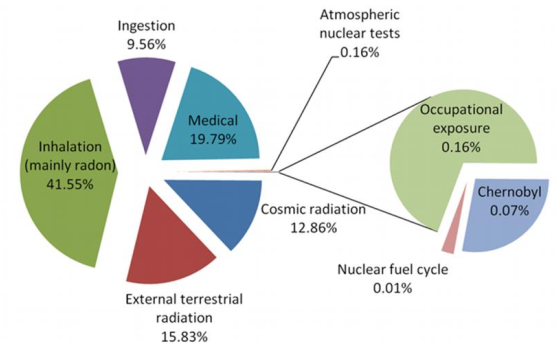
\includegraphics[scale=0.5]{2Introduction/RadioactiveDosePopulation.png}
\centering
\caption{Annual average distribution of the radioactive dose received by the population~\cite{IAEA}\label{fig:RadioactiveDosePopulation}.}
\end{figure}

\begin{table}[h]
\centering{}%
\begin{tabular}{lcc}
\toprule 
Radiation source & Eff. dose ($\milli\sievert/$yr) & Typical range ($\milli\sievert/$yr)\tabularnewline
\midrule
\midrule 
Cosmic (external) & $0.39$ & $0.3 - 1.0$ \tabularnewline
Terrestrial (external) & $0.48$ & $0.3-0.6$ \tabularnewline  
Inhalation (internal) & $1.26$ & $0.2-10$ \tabularnewline
Ingestion(internal) & $0.29$ & $0.2-0.8$ \tabularnewline
\midrule
Total & $2.42$ & $1-12.4$ \tabularnewline
\bottomrule
\end{tabular}
\caption{Annual average distribution of the effective dose received by the population due to natural radioactivity~\cite{UNSCEAR, CSN}.}
\label{tab:RadioactiveNaturalDosePopulation}
\end{table}

Since the discovery of radioactivity by Henri Becquerel in $1896$, lots of nuclear-based technologies were developed and applied to various fields such as Energy, Chemistry, Biology, Technology, Medicine, Industry, etc. Due to nuclear applications, a number of anthropogenic radioactive sources have emerged in society, resulting in radioactive elements released into the environment. It can be noticed in Figure \ref{fig:RadioactiveDosePopulation} that the most important part of the dose received by the population from artificial sources comes from medical practice. The growth of knowledge and the development of measurement techniques for radioactivity have provided evidence of the harmful effects of radioactivity on living organisms. This leads to the necessity of controlling the radiation to which the population is exposed, keeping it under safe limits. To accomplish this purpose, several organizations were created to propose recommendations for radiological protection to the different state organisms and governments at the international level. The main ones are:

\begin{enumerate}
\item{} The International Commission of Radiological Units and Measurements (ICRU) \cite{ICRU}, created during the first International Conference of Radiology held in London in 1925 to define concepts and units necessary to quantify the negative effects of radioactivity.

\item{} The International Commission on Radiological Protection (ICRP) \cite{ICRP}, created in 1928 by the International Society of Radiology (ISR) \cite{ISR}. The ICRP aims to make recommendations and provide guidance on different aspects of protection against radioactivity. The ICRP does not have the legal capacity to enforce its recommendations, but these are widely included in the legislation of most countries. %is fairly consistent with them.

\item{} The United Nations Scientific Committee on the Effects of Atomic Radiation (UNSCEAR) \cite{UNSCEAR}, created in 1955 with the goal of estimating and reporting the levels and effects of ionizing radiation on the population and the environment. These estimates are taken into account by governments worldwide to establish their safety standards.

\item{} The International Atomic Energy Agency (IAEA) \cite{IAEA}, created in 1957 to promote the peaceful use of nuclear energy and to avoid its use for military purposes such as nuclear weapons. Although established independently from the United Nations through its international treaty, the IAEA reports regularly to both the United Nations and the Security Council.

\item{} The European Atomic Energy Community (EURATOM), created in 1957, which is an international organization ruled by the EURATOM treaty. Its objective is to coordinate research programs for the peaceful use of nuclear energy and the sharing of knowledge, infrastructures and funding of nuclear energy.

\item{} The Nuclear Safety Council (CSN) \cite{CSN} of Spain, created in 1980, is the authority in Spain for nuclear safety and radiation protection. It has the objective of protecting employees, the general population and the environment from the harmful effects of ionizing radiation from anthropogenic origin. For this goal, the CSN ensures that nuclear and radioactive facilities are operated safely and establishes the preventive and corrective measures to be applied in radiological emergencies. The CSN manages two detector networks to control the levels of radioactivity in the environment and to assess the impact of radioactive facilities:

\begin{enumerate}
\item{} The network of automatic stations REA (Red de Estaciones Automáticas) \cite{REA}. The REA consists of several gamma detectors, distributed across the country as indicated in Figure \ref{subfig:REA}, which measure the radioactive dose in real time. The REA is employed for real-time detection of radiological issues to enable taking prompt safety measures.

\item{} The network of sampling stations REM (Red de Estaciones de Muestreo) \cite{REM}. The REM consists of a collection of points, shown in Figure \ref{subfig:REM}, from which samples are taken and measured in a laboratory. About twenty Spanish laboratories integrate this network. The objective of the REM is to characterize the concentration and evolution of radioisotopes present in the radioactive background of Spain and to quantify the impact of radioactive facilities on the environment.
\end{enumerate}

\begin{figure}
\centering
    \begin{subfigure}[b]{0.7\textwidth}
    \centering
    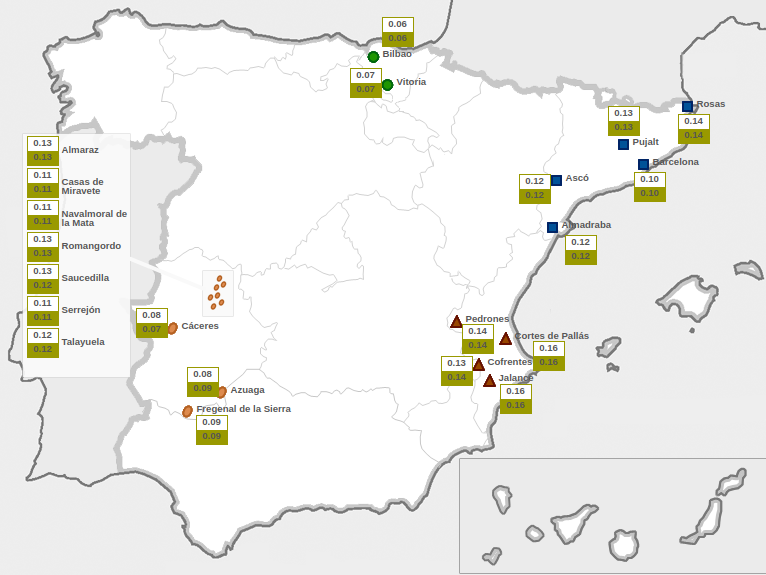
\includegraphics[width=\textwidth]{2Introduction/REA.png}  
        \caption{}\label{subfig:REA}
    \end{subfigure}
    \hfill
    \begin{subfigure}[b]{0.7\textwidth}
    \centering
    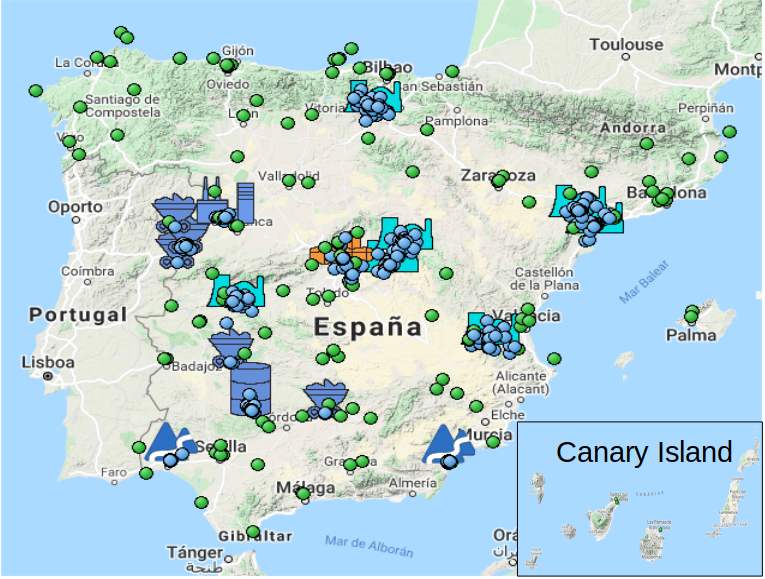
\includegraphics[width=\textwidth]{2Introduction/REM.png}  
    \caption{\label{subfig:REM}}
    \end{subfigure}
 \caption{Networks of automatic and sampling stations managed by the Spanish CSN. a) Measurement locations of the REA \cite{REA}. The white and green insets are the daily and monthly average of the gamma dose, respectively. b) Measurement locations of the REM \cite{REM}. Blue dots are locations near nuclear facilities, and green dots are locations uniformly distributed throughout the country.}
 \label{fig:NetworksCSN}
\end{figure}
%There are other networks that measure different parameters such as the concentration of $\ce{^{222}Ra}$ in the air. The measurements of all the networks complies with to the EUROTAM treaty \cite{100BqL}.

\end{enumerate}

The goal of the TRITIUM project is to develop a monitor capable of automatically measuring low levels of tritium in water in quasi-real-time\footnote{Quasi-real-time is an approximation of real-time measurements. It means a relatively small time, like less than $1~\hour$.}. This monitor is intended to be included in the REA.

Tritium is one of the radioactive isotopes routinely measured in REM tests. It is detected through the low-energy electrons produced in its beta decay, mainly using the Liquid Scintillation Counter technique (LSC). Due to the limitations of the current tritium detection techniques, described in section \ref{sec:StateOfTheArt}, the TRITIUM project was recently proposed with the objective of building a tritium detector based on scintillating fibres in contact with the water sample. The photons produced in these scintillating fibres are read out by photosensors, either photomultiplier tubes (PMTs) or silicon photomultipliers (SiPMs). The final emplacement of the TRITIUM monitor is a site close to the Arrocampo dam (Extremadura, Spain), whose water is used for the cooling system of the Almaraz nuclear power plant (NPP), located 4 km upstream from the Arrocampo dam. The monitor will be used to ensure that the tritium levels of the Arrocampo dam  water are below the legal limit of $100~\becquerel/\liter$ specified in the EURATOM Directive 2013/59/Euratom \cite{100BqL}. In addition, this will confirm the correct operation of the Almaraz NPP, since an increase of tritium activity released could indicate a malfunctioning of the reactor. This monitor could also be used in many different places with radioactive facilities like the future fusion power plants\footnote{The International Thermonuclear Experimental Reactor, ITER, will need up to several tens of kilograms of tritium to function, which corresponds to several $\tera\becquerel$ of activity.}, nuclear research facilities\footnote{Tritium is one of the main emissions from nuclear research facilities \cite{FERMILAB, BrookHavenNationalLaboratory}.} or tracking the pathway of tritium discharges to groundwater \cite{TrackingTritium}. 

Tritium is one of the most abundantly produced radioisotopes in an NPP, as it was verified in the United States Department of Energy (DOE) \cite{FiberDetector1a, FiberDetector1b}, in several research facilities in China \cite{CommonEmissionTritium} and places close to them (ground, surface and wastewater). Tritium is produced in the nuclear reactor cooling water system of NPPs by neutron capture of deuterium existing in the heavy water ($\ce{D_2 O}$), semi-heavy water ($\ce{H D O}$) or deuterium created by neutron capture in light water ($\ce{H_2 O}$). Tritium is finally released partially or totally into the environment in a quantity that depends on the reactor type, as shown in Table \ref{tab:TritiumEmisionsNPPs}. The most common form in which tritium is released into the environment is $\ce{HTO}$ \cite{CommonEmissionTritium}.
%All these processes have a large probability of happening due to the huge neutron flux, of the order of $10^{14} ~\ce{n} \, \cm^{-2} \second^{-1}$ in the nuclear reactor \cite{CrossSeccionNeutrons}

\begin{table}[htbp]
\centering{}%
\begin{tabular}{lcc}
\toprule 
Reactor type & Gaseous discharge ($\giga\becquerel/$y) & Liquid discharge ($\giga\becquerel/$y)\tabularnewline
\midrule
\midrule 
PWR & $3.70\cdot 10^{3}$ & $2.59\cdot 10^{4}$ \tabularnewline
BWR & $1.85\cdot 10^{3}$ & $3.70\cdot 10^{3}$ \tabularnewline
HWR & $7.40\cdot 10^{5}$ & $1.85\cdot 10^{5}$ \tabularnewline
GCR & $7.40\cdot 10^{3}$ & $1.11\cdot 10^{4}$ \tabularnewline
\bottomrule
\end{tabular}
\caption{Emission of tritium per year from different types of nuclear reactors: Pressurized Water Reactor (PWR), Boiling Water Reactor (BWR), Heavy Water Reactor (HWR) and Gas-Cooled Reactor (GCR) \cite{CommonEmissionTritium}.}
\label{tab:TritiumEmisionsNPPs}
\end{table}

NPPs are operational for more than 60 years and, nowadays, they are essential for providing a large part of the electric power used all over the world (more than $20\%$ in Spain \cite{PercentageEnergySpain} and more than $10\%$ in the world \cite{PercentageEnergyWorld}). Although the Spanish government is planning to progressively shut all NPPs down, there are other countries like China \cite{60ReactorsChina} or the United States \cite{35MillionsUSA} that promote their use. NPPs are a profitable investment since they are one of the cheapest sources of energy production. Their energy production rate is stable since it does not depend on meteorological conditions. Moreover, NPPs do not emit greenhouse gases. Although there are alternative energy sources which are being developed quickly (photovoltaic, wind, tidal energy, etc.), as well as other concepts of energy production and saving (local production, energy efficiency, smart cities, etc.), they are currently not enough to cover the population needs. However, NPPs have some important drawbacks such as contamination of fresh water from uranium mining, nuclear waste, nuclear proliferation and the risk of radioactive contamination from accidents as happened in the past: Chernobyl, Fukushima and Three Mile Island \cite{ThreeMileIsland}. In any case, world nuclear energy production is most likely not going to be stopped in the next decade. In fact, the United States Energy Information Administration (EIA) expects a future increase of nuclear energy production \cite{EIAOutlook}. Therefore, safety is not a negotiable aspect and there must be a development of safeguards, like alarm systems, that warn of any malfunction of NPPs. 

%which is normally done by liquid scintillation counter technic (LSC). This technic has a very good detection capability and precision but it has the inconvenient of providing a delayed results of about 1-2 days or even more. Liquid scintillation technique for the tritium measurement will be presented in section \ref{sec:StateOfTheArt}. 
	%\newpage
	
	\section{Tritium Properties and Radiological Hazards}\label{sec:TritiumProperties}
	Tritium is the only radioactive isotope of hydrogen. It was first time produced in $1934$ from neutron capture of deuterium by Ernest Rutherford, Mark Oliphant and Paul Harteck \cite{TritiumDiscovery} and it was first time isolated in 1939 by Luis Walter Alvarez and Robert Cornog \cite{TritiumIsolate}, who checked that tritium is a radiactive element. 

Tritium is naturally produced in the environment through the interaction of cosmics rays and gaseous elements of the upper atmosphere like nitrogen ($\ce{^{14}N}(\ce{n},\ce{^{3}H})\ce{^{12}C}$) \cite{TritiumHandling} and oxigen ($\ce{^{16}O}(\ce{n},\ce{^{3}H})\ce{^{14}N}$) \cite{OxigenTritium}. Around 99\% of this tritium form water (\ce{HTO}) and reaches the earth's surface as rain with an estimated produccion rate of $4\cdot 10^6 ~\curie/$yr ($1.48 \cdot 10^8 ~\giga\becquerel/$yr), producing a tritium concentration of $0.6-1.2~\becquerel/\liter$ in precipitation \cite{CommonEmissionTritium, TritiumHandling}. 

Tritium can be produced artificially in the environment from different anthropogenic sources \cite{CommonEmissionTritium, TritiumHandling}. There is a large amount of tritium which was produced in military nuclear test explosions between 1945 and 1975, with an estimated total production of $8 \cdot 10^9~\curie$ ($2.96 \cdot 10^{11}~\giga\becquerel$) and a part of which remains to the date. In these nuclear explosions, tritium was produced mainly from the nuclear reactions $\ce{^{14}N}(\ce{n},\ce{^{3}H})\ce{^{12}C}$ and $\ce{^{2}H}(\ce{n},\gamma)\ce{^{3}H}$. Tritium can be also produced by commercial producers of radioluminiscent and neutron generator devices ($1 \cdot 10^6~\curie/$yr), nuclear power and defense industries (around $2 \cdot 10^6~\curie/$yr) and several research facilities and nuclear reactor for energy production ($2 \cdot 10^6 \curie/\giga\watt$yr), whose main production cross sections are shown in Table \ref{tab:NuclearReactionsTritiumProduction}: 

\begin{table}[htbp]
\begin{center}
\begin{tabular}{|c|c|c|c|}
\hline
Element & Origin & Nuclear reaction & Cross section ($\barn$)\\
\hline \hline \hline
$\ce{^{2}_{1}H}$ & Water coolant & $\ce{^{2}_{1}H}(\ce{n},\gamma)\ce{^{3}_{1}H}$ & $5.2 \cdot{} 10^{-4}$ \\ \hline
$\ce{^{3}_{2}He}$ & Helium coolant & $\ce{^{3}_{2}He}(\ce{n},\ce{p})\ce{^{3}_{1}H}$ & $5330$ \\ \hline
$\ce{^{6}_{3}Li}$ & Moderator & $\ce{^{6}_{3}Li}(\ce{n},\alpha)\ce{^{3}_{1}H}$ & $940$ \\ \hline
$\ce{^{10}_{5}B}$ & \parbox{8em}{\centering Moderator,\\ control rods} & $\ce{^{10}_{5}B}(\ce{n},2\alpha)\ce{^{3}_{1}H}$ & $3835$ \\ 
\hline
\end{tabular}
\caption{Most common nuclear reactions of artificial tritium production~\cite{CommonEmissionTritium}}
\label{tab:NuclearReactionsTritiumProduction}
\end{center}
\end{table}

%\begin{equation}
%\ce{^{2}_{1}H}(\ce{n},\gamma)\ce{^{3}_{1}H} \qquad \sigma= 5.2 \cdot{} 10^{-4}~\barn  ~~~\cite{CommonEmissionTritium}
%\label{eq:capneuH2}
%\end{equation}

%\begin{equation}
%\ce{^{3}_{2}He}(\ce{n},\ce{p})\ce{^{3}_{1}H} \qquad \sigma= 5330~\barn ~~~\cite{CommonEmissionTritium}
%\label{eq:capneuHe3}
%\end{equation}

%\begin{equation}
%\ce{^{6}_{3}Li}(\ce{n},\alpha)\ce{^{3}_{1}H} \qquad \sigma= 940~\barn ~~~\cite{CommonEmissionTritium}
%\label{eq:capneuLi6}
%\end{equation}

%%\begin{equation}
%%\ce{^{7}_{3}Li}(\ce{n},\alpha)\ce{^{3}_{1}He} + \ce{n} ~~~\cite{CommonEmissionTritium}
%%\label{capneuLi7}
%%\end{equation}

%\begin{equation}
%\ce{^{10}_{5}B}(\ce{n},2\alpha)\ce{^{3}_{1}H} \qquad \sigma= 3835~\barn ~~~\cite{CommonEmissionTritium}
%\label{eq:capneuB10}
%\end{equation}

%\begin{equation}
%\ce{^{11}_{5}B}(\ce{n},2\alpha)\ce{^{3}_{1}H} + n ~~~\cite{CommonEmissionTritium}
%\label{capneuB11}
%\end{equation}
%$\eqref{capneuLi6}$ para referenciar ecuaciones

%There are two more nuclear reaction with which we can produce tritium:

%\begin{equation}
%\ce{^{1}_1 H} (2 \cdot{} \ce{n},\ce{p})\ce{^{3}_1 H}
%\label{doblecapneuH}
%\end{equation}

%\begin{equation}
%\ce{^{2}_1 H}(\ce{n},\gamma)\ce{^{3}_1 H}
%\label{capneuD}
%\end{equation}

Tritium levels in the environment when anthropological radioactive sources are not involved are between $1$ and $4~\becquerel/\liter$. This is a higher value than the expected due to the cosmogenic background levels ($0.6-1.2~\becquerel/\liter$, previously mentioned) \cite{FranceTritiumEnvironment}. It can be explained by the consequences of nuclear weapons tests.

Tritium levels in rivers around a nuclear facility are between $1$ and $10~\becquerel/\liter$ and even between $20$ and $50~\becquerel/\liter$ at the water discharge site of NPPs \cite{FranceTritiumEnvironment}, where the produced tritium is partially or totally released into the environment, mainly in the $\ce{HTO}$ water form.

The effect of NPP on tritium levels can be observed using the public measurements of the REM, explained in the section \ref{sec:Introduction}. For example, in the case of Cofrentes, which is the closest nuclear power plant to Valencia and the one in whose measurements are involved LARAM\footnote{LARAM is a Valencia laboratory specialized in environmental radioactivity measurements}, the tritium levels in the river are measured in three different places, marked on the map shwon in Figure \ref{fig:SamplingLocations}. The first place, P1, is located in the river, $6~\kilo\meter$ upstream from the NPP, the second place, P2, is located $1~\kilo\meter$ downstream and the third place, P3, is located $5~\kilo\meter$ downstream. The level of Tritium measured in these three locations is shown over time in Figures \ref{fig:TritiumL6kB}, \ref{fig:TritiumL1kA} and \ref{fig:TritiumL5kA} respectively.

\begin{figure}[hbtp]
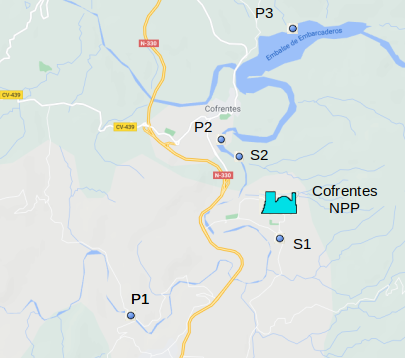
\includegraphics[scale=0.5]{2Introduction/CofrentesMaps.png}
\centering
\caption{Tritium sampling locations around Cofrentes NPP.\label{fig:SamplingLocations}}
\end{figure}

\begin{figure}[hbtp]
 \centering
  \subfloat[Tritium activity $6~\kilo\meter$ upstream.]{
  \label{fig:TritiumL6kB}
    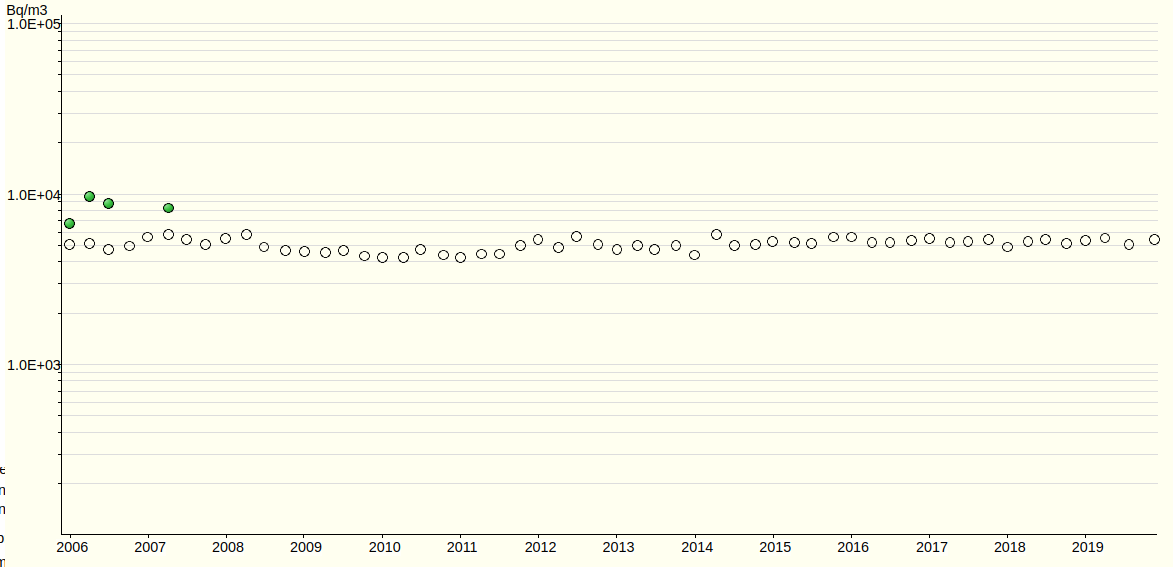
\includegraphics[width=0.47\textwidth]{2Introduction/6km_before.png}}
    %\newline
      \subfloat[Tritium activity $1~\kilo\meter$ downstream.]{
   \label{fig:TritiumL1kA}
    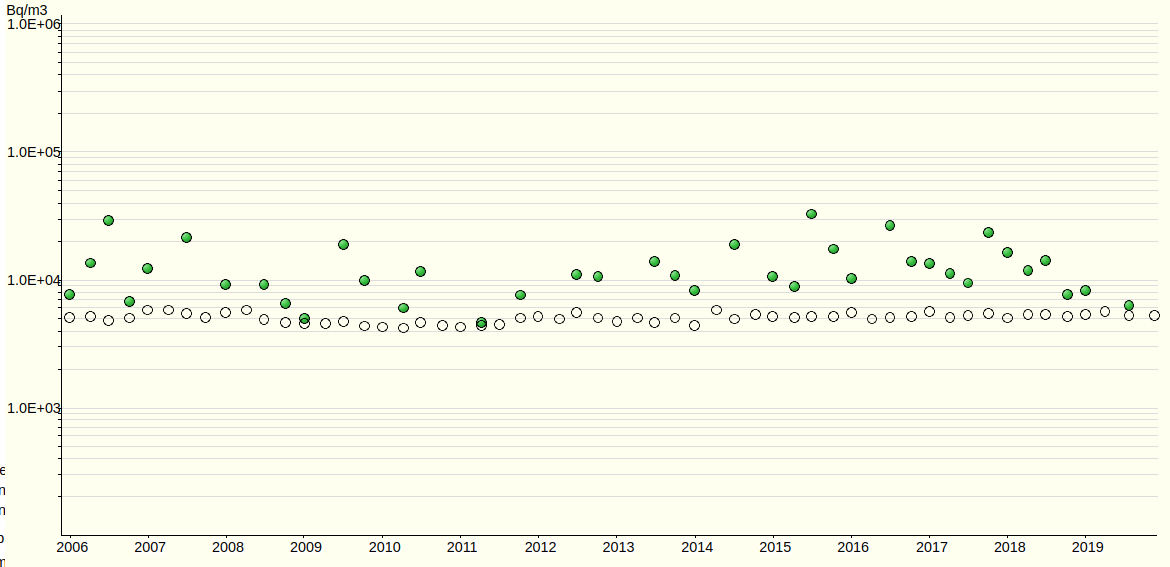
\includegraphics[width=0.47\textwidth]{2Introduction/1km_after.png}}
    \newline
  \subfloat[Tritium activity $5~\kilo\meter$ downstream.]{
  \label{fig:TritiumL5kA}
    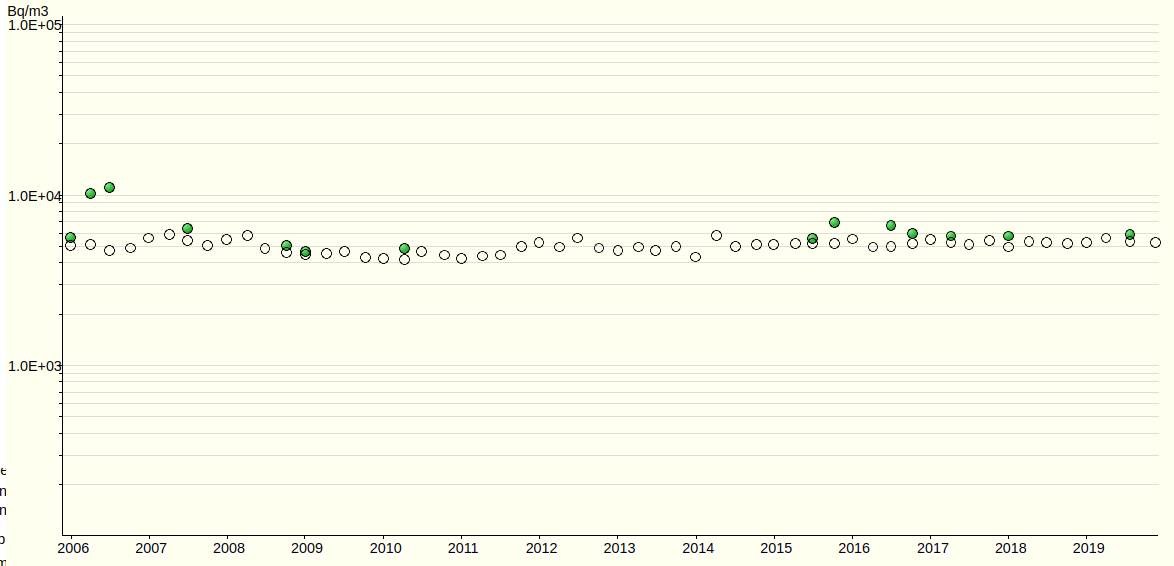
\includegraphics[width=0.47\textwidth]{2Introduction/5km_after.png}}
 \caption{Tritium activity levels in surface water around Cofrentes NPP from January $2006$ to November $2019$. The white points are used for the detection limit and the green points are used for the measured activity, when it is above the detection limit.~\cite{REM}}
 \label{fig:MeasurementsCofrentesSurface}
\end{figure}

In these figures, the detection limit and the measured activity are shown using white dots and green dots respectively. The measured activity is only displayed when it is larger than the corresponding detection limit. As it can be seen, the tritium level in the river increases due to the discharge of the NPP and it is diluted again after $4~\kilo\meter$ downstream. 

Two additional measurements of the tritium level in groundwater have been included, points S1 and S2 on the map in Figure \ref{fig:SamplingLocations}, which are located $1~\kilo\meter$ before and $1~\kilo\meter$ after the NPP. Both tritium levels are shown in the figure \ref{fig:TritiumLG1kB} and \ref{fig:TritiumLG1kA} respectively, where it can be verified that the nuclear power plant has not affected them.

\begin{figure}[hbtp]
 \centering
      \subfloat[Tritium activity $1~\kilo\meter$ before NPP.]{
   \label{fig:TritiumLG1kB}
    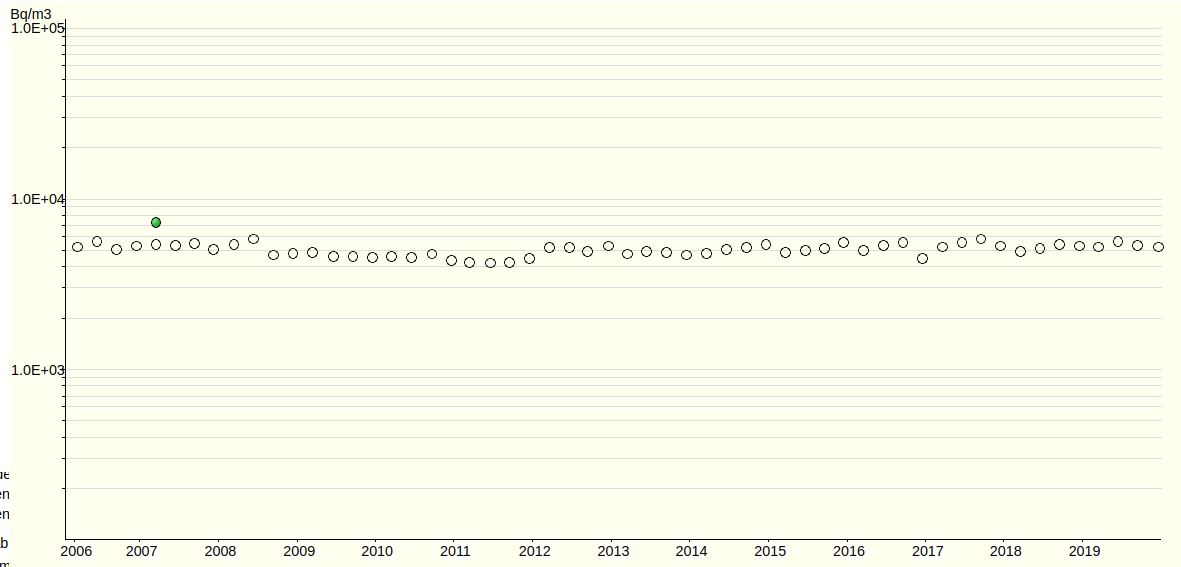
\includegraphics[width=0.47\textwidth]{2Introduction/Subterranea_before.png}}
    %\newline
  \subfloat[Tritium activity $1~\kilo\meter$ after NPP.]{
  \label{fig:TritiumLG1kA}
    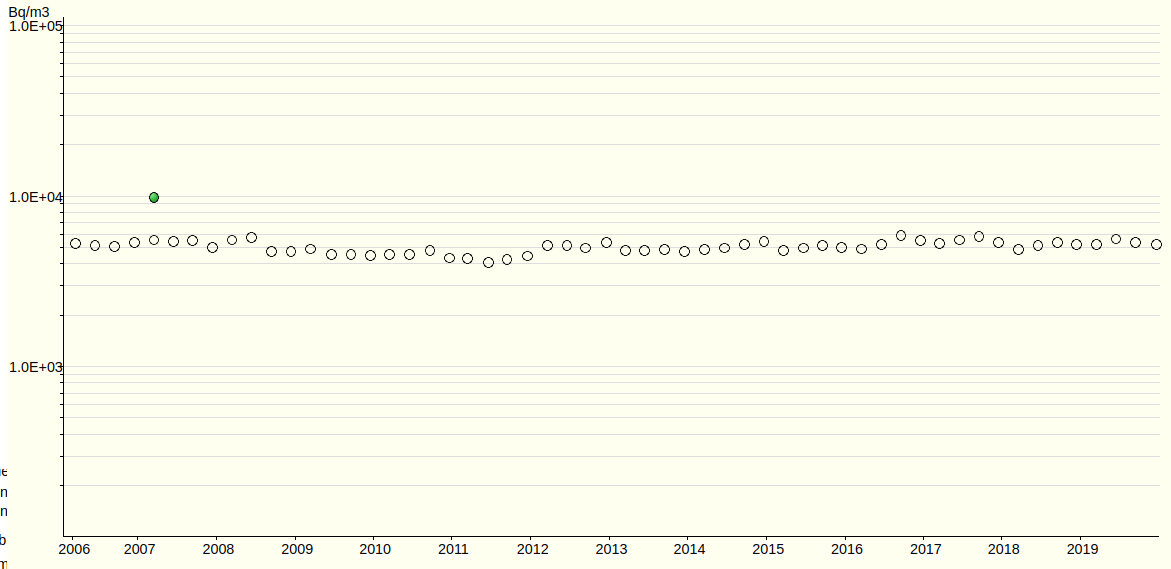
\includegraphics[width=0.47\textwidth]{2Introduction/Subterranea_1_km_later.png}}
 \caption{Tritium activity levels in groundwater around Cofrentes NPP from January $2006$ to November $2019$.~\cite{REM}}
 \label{fig:MeasurementsCofrentesGroundWater}
\end{figure}

It is important to note that, although environmental tritium levels have been affected due to NPP, these levels are below the legal limit. The maximum level of tritium measured since of January 2, 2006 is around $32~\becquerel/\liter$, below to the legal limit in Europe, $100~\becquerel/\liter$.

Tritium is a radioactive element whose half-life time is $T_{1/2}= 12.32$ years. It has one proton and two neutrons and decays exclusively through $\beta$ radiation. It decay $100\%$ directly to the ground state of Helium ($\ce{^{3}_{2}He}$), which is a stable nuclei, thorugh the decay scheme of equation \ref{eq:TritiumDecay}:

%In this decay, one neutron of tritium is transformed transformed into a proton, an electron and an electron-antineutrino, according to the following decay scheme:

%\begin{equation}
%\ce{n} \longrightarrow \ce{p}  + \ce{e^-}  + \ce{\overline{\nu}_e}
%\label{eq:BetaDecay}
%\end{equation}



\begin{equation}
\ce{^{3}_{1}H} \longrightarrow \ce{^{3}_{2}He}  + \ce{e^-}  + \ce{\overline{\nu}_e}
\label{eq:TritiumDecay}
\end{equation}

In Figure \ref{fig:TritiumDecay} the scheme of tritium energy levels is shown. In this decay it is not possible to detect the neutrino because of its extremely weak interaction with matter ($\sigma \propto 10^{-42} ~ \cm^2$ \cite{CrossSeccionNeutrino}) and, since $\ce{^{3}He}$ has a much larger mass than electrons and neutrinos, by conservation of energy and momentum, the energy that is taken by this daughter nucleus is very small. Therefore, the detection of tritium is through its decay electron. 

\begin{figure}[hbtp]
 \centering
  \subfloat[Tritium energy levels \cite{TritiumDecayEnergyLevels}]{
   \label{fig:Energy_levels}
    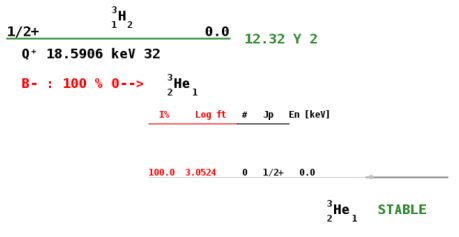
\includegraphics[width=0.60\textwidth]{2Introduction/esquema_niveles_energeticos.png}}
  \subfloat[Graphic representation of tritium decay \cite{TritiumDecayImage}]{
   \label{fig:GraphicDesintegration}
    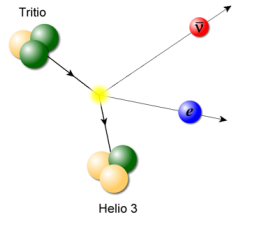
\includegraphics[width=0.40\textwidth]{2Introduction/representacion_desintegracion.png}}
 \caption{Tritium decay}
 \label{fig:TritiumDecay}
\end{figure}

The energy released in the tritium decay is $Q_\beta=18.6~\keV$, which is divided between the decay products. Therefore, the energy spectrum of the decay electrons is a continuum with a maximum value of $18,6~\keV$, as shown in Figure \ref{fig:TritiumDecaySpectrum}. This energy spectrum has an average of $5.7~\keV$ and the most likely value is slightly below, around $4.5~\keV$.

\begin{figure}[hbtp]
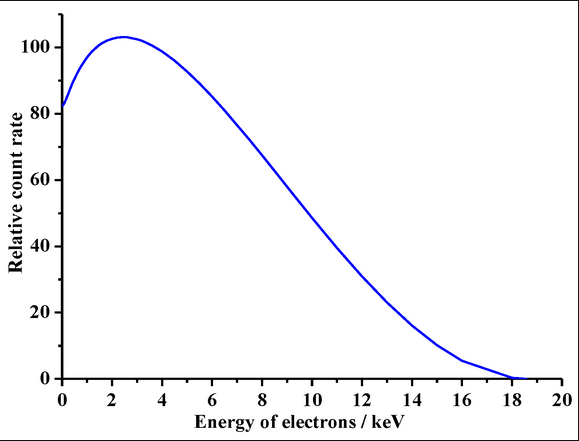
\includegraphics[scale=0.6]{2Introduction/Espectro_tritio.png}
\centering
\caption{Energy spectrum of tritium electrons ~\cite{TritiumEspectrum}\label{fig:TritiumDecaySpectrum}}
\end{figure}

%We have to keep in mind that, although the helium isotope is stable, it will be exited immediately after this decay. As a consequence, after the tritium $\beta^-$ decay, we will have a subsequent dexcitation of the $\ce{^{3}He}$ which will produce photons, $\gamma$, with several well-defined energies that correspond to their energy levels, X-rays\footnote{X-rays are photons whose wavelength are between 0.01 nm and 10 nm. They are produced by nuclear deexitation.}. It will not affect our tritium measurement because, as we will see in Section  \ref{}, the probability of detecting X-rays with the photosensor that will be used is practically negligible.

%Los rayos X son una radiación electromagnética de la misma naturaleza que las ondas de radio, las ondas de microondas, los rayos infrarrojos, la luz visible, los rayos ultravioleta y los rayos gamma. La diferencia fundamental con los rayos gamma es su origen: los rayos gamma son radiaciones de origen nuclear que se producen por la desexcitación de un nucleón de un nivel excitado a otro de menor energía y en la desintegración de isótopos radiactivos, mientras que los rayos X surgen de fenómenos extranucleares, a nivel de la órbita electrónica, fundamentalmente producidos por desaceleración de electrones. La energía de los rayos X en general se encuentra entre la radiación ultravioleta y los rayos gamma producidos naturalmente. Los rayos X son una radiación ionizante porque al interactuar con la materia produce la ionización de los átomos de la misma, es decir, origina partículas con carga (iones). 

The releasing energy of the tritium decay, is very little. In fact, it is the radioactive isotope with the lowest energy released in its $\beta$ disintegration \cite{TritiumHandling}. Consequently, the $\beta$ particle which is emitted in this tritium decay will have a very small mean free path as it is shown in Table \ref{tab:MeanFreePathTritium}.

\begin{table}[htbp]
\begin{center}
\begin{tabular}{|c|c|c|}
\hline
Material & P. Depth ($5.7~\keV$) & P. Depth ($18.6~\keV$)\\
\hline \hline \hline
$\ce{\ce{^{3}_{1}H_2}}$ & 0.26 cm & 3.2 cm \\ \hline
Air & 0.036 cm & 0.45 cm \\ \hline
\parbox{10em}{\centering Water, soft tissue\\  (solid matter whose \\  density is $1~\gram\cdot\cm^{-3}$)} & 0.42 $\mu\meter$ & 5.2 $\mu\meter$ \\ \hline
\end{tabular}
\caption{Penetration depth for decay electron of mean ($5,7~\keV$) and maximum ($18,6~\keV$) energies in different media (tritium gas and air at standard conditions of temperature ($273~\kelvin$) and preassure ($1$ atm), STP, and water)~\cite{MeanFreePathDocument}}.
\label{tab:MeanFreePathTritium}
\end{center}
\end{table}

This short mean free path is a major issue in tritium detection, as it makes more difficult the electron detection, which will require a highly sensitive detector. However, it means that the tritium electrons has a low penetration in our body and easily stopped with our clothes or laboratory gloves, resulting in a low radiological hazard of external tritium.

Nevertheless, the danger of tritium increases when it is ingested or inhaled since it can bind anywhere that hydrogen can and perform the same chemical reactions, sometimes with higher rate if the tritium concentration is high enough to catalyze the reaction. 

Tritium can be absorbed in our body in three different ways, gaseous tritium (mainly HT), tritiated water (mainly HTO) and organically bound tritium (called OBT).

The gaseous tritium, which is normally found mixed in the air, is the least important since less than a $3-5 \cdot{} 10^{-3}~\%$ is absorbed, which is insignificant \cite{TritiumHandling}. However, it can be transformed into tritiated water through the oxidation and exchange reactions shown in the chemical schemes of equations \ref{eq:OxidationExchange}, which has a more important effect on health \cite{TritiumHandling}:

\begin{equation}
\begin{split}
& Oxidation: \qquad \qquad \qquad \qquad \qquad \qquad Exchange\\
& 2\cdot{}\ce{HT} + \ce{O_2} \rightarrow 2 \cdot{} \ce{HTO} ~ \quad \qquad \qquad \qquad \ce{HT} + \ce{H_2 O} \rightarrow \ce{H_2} + \ce{HTO}\\
& 2\cdot{}\ce{T_2} + \ce{O_2} \rightarrow 2 \cdot{} \ce{T_2 O} \qquad \qquad \qquad \qquad \ce{T_2} + \ce{H_2 O} \rightarrow \ce{HT} + \ce{HTO}
\label{eq:OxidationExchange}
\end{split}
\end{equation}

Tritiated water, which is normally found in drinking water or water in food, has a larger impact since the $99\%$ of it is absorbed \cite{TritiumHandling}. In addition, its biological life time of it is around $9.5$ days ($\pm50\%$), time during which tritium will remain in our body \cite{TritiumHandling, FranceTritiumEnvironment, EstimationTritiumDosi}.

This time corresponds to the water cycle in the body and, like this, it can vary due to various external parameters such as temperature, humidity, drinking habits, etc. or reduced with the use of diuretics \cite{TritiumHandling}.

Organically bound tritium, normally found in food, generally forms a covalent bond with a carbon and and it corresponds to $5-10~\%$ of tritium absorbed in the body. Although it is absorbed in less quantity in the body than tritiated water, it can be more dangerous since it has a longer biological life time. The biological life time of this tritium type depends on the affinity of the organic molecule with the different biological tissues and it can vary from tens of days to hundreds of days (larger than the ICRP estimate) \cite{FranceTritiumEnvironment, EstimationTritiumDosi, EstimationTritiumDosiRats, EstimationTritiumDosiKangarooRats}.

There are many studies showing that tritium in living matter can cause the same effects than X-rays or $\gamma$ rays, which are mutations, tumors, cancer, genetic effects, reproductive effects, etc \cite{StraumeTritiumHazard, RytoemaaTritiumHazard}. In fact, the consequences of tritium radiation can be worse than a similar $\gamma$ radiations since its biological efficiency\footnote{The biological efficiency is used to quantify the damage produced in the living cells due to an external radiation.} is two or three times larger \cite{StraumeTritiumHazard}.

In summary, tritium is a naturally occurring radioactive element that can affect health if it is released excessively. Because of that, each country has developed a legislation, shown in section \ref{sec:Legislation}, to manage the release of tritium and ensure that these background levels are safe for health.



%Tritium has different physical properties than other natural isotopes of the hydrogen like different boiling points as shown in Table \ref{tab:BoilingPoints} or the property of self-radiolysis which only happens when radioactive elements are involved. In the case of tritium dissolved in water, it is normally found forming the $\ce{HTO}$ molecule. There, the auto-radiolysis ocurrs because the energy released in tritium decay is larger than the energy bond of oxigen and hydrogen in water molecules ($5.2~\eV$) or the ionization energy of water molecules ($12.6~\eV$) so it can break up these molecules \cite{AutoRadyolisis}. Due to the auto-radiolysis, some radicals appear in the water, increasing its corrosivity. It is a fact that we have to take into account when choosing the materials that will make up the TRITIUM detector.

%\begin{table}[htbp]
%\begin{center}
%\begin{tabular}{|l|l|l|}
%\hline
%Molecule & Boiling point (for gases) ($\kelvin$) & oxidation form\\
%\hline \hline \hline
%$\ce{H_2}$ & 20.39 & $\ce{H_2 O}$ \\ \hline
%$\ce{HD}$ & 22.14 & $\ce{HDO}$ \\ \hline
%$\ce{HT}$ & 22.92 & $\ce{HTO}$ \\ \hline
%$\ce{D_2}$ & 23.66 & $\ce{D_2 O}$ \\ \hline
%$\ce{DT}$ & 24.38 & $\ce{DTO}$ \\ \hline
%$\ce{T_2}$ & 25.04 & $\ce{T_2 O}$ \\ \hline
%\end{tabular}
%\caption{Gas molecules of hydrogen isotopes and their boiling point and oxidation form.~\cite{}}
%\label{tab:BoilingPoints}
%\end{center}
%\end{table}

%Although tritium has different physical properties it has almost the same chemical behaviour than other hydrogen isotopes. Tritium, like hydrogen, is a gas at STP forming a two-atom molecules which can be $\ce{HT}$, $\ce{DT}$ and $\ce{T_2}$. 


%Due to this chemical similarity tritiated water can perform the same chemical processes than non-radiactive water, sometimes with higher rate if the tritium concentration is high enough to catalyze the reaction. Its biological hazard comes from this chemical similarity since tritiated water is able to substitute normal water in human body. 

	%\newpage
	
	\section{Current Legislation}\label{sec:Legislation}
	Due to the radiological risk of tritium, which has been shown in section \ref{sec:TritiumProperties}, it is important to develop a legislation that limits the release of tritium to the environment ensuring that the levels are below a safe value for health.

The guidelines that impose the limit of radioactive elements in drinking water for many countries are based on the radiation protection methodology developed by the ICRP \cite{ICRP_GL} and the recommendations of the world health organization, WHO \cite{WHO_GL}.

The objective of the international radiation methodology is to  protect people and the environment from the negative effects of ionizing radiations without limiting beneficial activities that involve radiation exposure. It is based on three main points, which are the justification (the benefit from radiological exposure must outweigh the detriment to health that it causes), the ALARA principle, "As Low As Reasonably Achievable" (the radiological exposure must be kept as low as possible considering social and economic factors) and dose limitation (limit that must never be exceeded).

While the ICRP recommends a maximum dose of $1~\milli\sievert/$yr, excluding the natural background and medical interventions, the WHO is more conservative, recommending a maximum dose of $0.1~\milli\sievert/$yr, which correspond to less than $5\%$ of the annual dose due to background radiation, $2.42~\milli\sievert/$year, Table \ref{tab:RadioactiveNaturalDosePopulation}.

The guideline reference level of each radionuclide in drinking water, GL, is usually calculated from these recomendations using the equation \ref{eq:Guideline}

\begin{equation}
GL = \frac{RDL}{DCF \cdot{} q}
\label{eq:Guideline}
\end{equation}

Where RDL is the reference dose level, DCF is the dose conversion factor (the normal used value for tritium is $1.8*10^{-11}~\sievert\becquerel$, provided by ICRP \cite{ICRP_factor}) and q is an estimation of the annual volume of drinking water consumed (normally assumed two liters per day, $730~\liter/$yr).

The GLD calculated for tritium in drinking water according to the ICRP and WHO recommendations is $76103~\becquerel/\liter$ and $7610~\becquerel/\liter$  respectively. It means that tritiated water with activities below these values is not harmful to health.

Based on these recommendations, each country has created organizations in charge of developing its own legislation on radionuclide limits. In Spain, the responsible organization of this task is the CSN.

Most of the countries in the world implement the RDL of $0.1~\milli\sievert/$yr recommended by the WHO. The legal limit for tritium in drinking water in this case is $76.103~\becquerel/\liter$  but it is often approximated in different ways. Some countries like Switzerland \cite{Switzerland_GL} or some organizations like the WHO \cite{WHO_GL} rounded this value to $10,000~\becquerel/\liter$. Others like some countries of Canada, such as Ontario and Québec, truncate this value to the first number $7,000~\becquerel/\liter$ \cite{Ontario_GL, Quebec_GL}. There are other countries like Russia which use the much more accurate approximation value of $7,700~\becquerel/\liter$ \cite{Russia_GL}.

There are other countries like Australia that prefer to implement the RDL of $1~\milli\sievert/$yr, recommended by the ICRP, whose legal limit is $76.103~\becquerel/\liter$ \cite{Australia_GL}. Other countries like Finland are based in the ICRP recommendations and use only the middle of this value, $0.5~\milli\sievert/$yr, whose value is rounded to a legal limit of $30,000~\becquerel/\liter$ for tritium in drinking water \cite{Finland_GL}.

There are two different exceptions to these recommendations:
\begin{enumerate}
\item{} On the one hand, most of the USA countires, such as California, use a RDL of $4~\milli\rem~(0.04~\milli\sievert)$, which corresponds to a legal limit of $20~\nano\curie/\liter~(740~\becquerel/\liter)$ \cite{California_GL}. This value was proposed by the United States Environmental Protection Agency (US EPA) as a result of an analysis of the available information \cite{USEPA_GL}.

\item{} On the other hand, most of the EU countries, such as France, Germany or Spain, impose an GL of $100~\becquerel/\liter$, which is one of the most restrictive limit in the world \cite{France_GL, Germany_GL, Spain_GL}. This value arise from the consideration that it is an indicator of the presence of other radionuclides more dangerous than tritium. These limits are fixed by the EURATOM Council Directive \cite{EURATOM_GL}. 
\end{enumerate}

All limits mentioned in this section are summarized in table \ref{tab:LegalLimitTritium}.

\begin{table}[htbp]
\begin{center}
\begin{tabular}{|c|c|}
\hline
Country/Agency & Legal limit of tritium ($\becquerel/\liter$)\\
\hline \hline \hline
ICRP & $76,103$ \\ \hline
WHO & $10,000$ \\ \hline
Switzerland & $10,000$ \\ \hline
Canada & $7,000$ \\ \hline
Russia & $7,700$ \\ \hline
Australia & $76,103$ \\ \hline
Finland & $30,000$ \\ \hline
United States & $740$ \\ \hline
European Union & $100$ \\ \hline
\end{tabular}
\caption{Legal limit of tritium in drinking water stablished in each country.}
\label{tab:LegalLimitTritium}
\end{center}
\end{table} 
	%\newpage
	
	\section{This Thesis}\label{sec:ThisThesis}
	This thesis is divided into nine different chapters that structure the information as follows:

\begin{enumerate}
\item{} \textbf{Chapter 1} provides a brief introduction to tritium detection, reports some important properties of tritium, and discusses the current legislation that limits tritium levels for human consumption in many countries around the world. 

\item{} \textbf{Chapter 2} describes the State-of-the-Art of tritium detection and shortly introduces the TRITIUM project. 

\item{} \textbf{Chapter 3} outlines the different parts of the TRITIUM monitor, which are the ultrapure water system, the background rejection system (consisting of the lead shielding and the active veto)  and the tritium detector. 

\item{} \textbf{Chapter 4} reports the calibrations of the different parts of the TRITIUM monitor and describes the developments aimed at improving the efficiency of tritium detection. 

\item{} \textbf{Chapter 5} details the geometrical configuration of the different prototypes built in the TRITIUM project. 

\item{} \textbf{Chapter 6} details the Monte Carlo simulations performed in the TRITIUM project. 

\item {} \textbf{Chapter 7} and \textbf{Chapter 8} report the results  achieved for the built prototypes and the simulations carried out, respectively. 

\item{} \textbf{Chapter 9} summarizes the most important results achieved in this work.

\end{enumerate}


	\newpage
	
\chapter{Tritium Detection Systems}\label{chap:TritiumDetection}
	
	\section{Tritium Detection State-of-the-Art}\label{sec:StateOfTheArt}
	Measurement of tritium activity is one of the routine environmental controls that are carried out in the vicinity of nuclear research facilities and nuclear power plants during their energy production lifetime. This measurement is carried out with different available technologies according to the state of the art of tritium detection. The most employed techniques are summarized in Table \ref{tab:DifferentThecnics}. Nowadays, the most used technique for measuring tritium in water is liquid scintillator counting (LSC). This technique consists of mixing a liquid sample (some millilitres for environmental measurements or less for higher activities) with liquid scintillator. This mixture is usually made in a ratio of 50:50 but it depends on the detection system and the activity of the samples \cite{LSCothers, Hofstetter1}. In this technique, the $\beta$ particles emitted from the sample excite the molecular energy levels of the liquid scintillator which promptly decays emitting several photons with a well-known energy (fluorescence), usually in the visible spectrum. Finally, these photons are detected with photosensors which convert the optical signal into a measurable electrical charge. The liquid scintillator technique has a very good detection sensitivity for low activity levels of tritiated water ($<1~\becquerel/\liter$) \cite{0.6Bq_L} but has the disadvantage of long measurement time (up to 2 days) and production of chemical waste, since liquid scintillators contain toluene which is toxic. In addition, the LSC technique requires special staff for sampling, a chain of custody and laboratory analysis which require economic and time resources. In order to overcome these difficulties, efforts were made to build a tritium monitor based on LSC which did not led a low enough minimum detectable activity (MDA) \cite{OnlineLSC}. 

{\renewcommand{\arraystretch}{1.8}
\begin{table}[htbp]
\centering{}%
\begin{tabular}{lcccc}
\toprule 
 & LSC & IC & Calorimetry & BIXS \tabularnewline
\midrule
\midrule 
\parbox{5em}{Measured\\ quantity} & \parbox{5em}{\centering Scintillation\\ photons} &  \parbox{5em}{\centering Ionization\\ current} & Heat & X-rays \tabularnewline
MDA & $\sim\becquerel$ & $10-100~\kilo\becquerel$ & $\sim~\giga\becquerel$ & $\sim~\mega\becquerel$ \tabularnewline
Sample state & Liquid & Gas, vapor & All & All \tabularnewline
\bottomrule
\end{tabular}
\caption{State-of-the-art tritium detection techniques. This table shows the measured quantity, the minimum detectable activity (MDA) and the sample form for four different techniques, liquid scintillator counting (LSC), ionization chamber (IC), calorimetry and beta induced X-ray spectrometry (BIXS).}
\label{tab:DifferentThecnics}
\end{table}}

The ionization chamber technique (IC) consists of an ionization chamber filled with gas (sample) which contains electrodes that collect the ionization current produced by the $\beta$ radiation in the gas. This is a simple and fast system, but it has a high MDA ($> 10~\kilo\becquerel$) and requires samples in a state of gas or steam \cite{IonizationChamber1, IonizationChamber2}. The IC technique also requires sample conditioning, chain of custody and laboratory analysis. 

The calorimetry method is based on the measurement of the heat generated in the detection medium (normally platinum) \cite{Calorimeter1, Calorimeter2}. The disadvantages of this technique are its high MDA (of the order of a $\giga\becquerel$) and the requirement of a long measurement time (2 days or more).

The Beta Induced X-ray Spectrometry (BIXS) is based on the measurement of the bremsstrahlung radiation produced by tritium decay electrons by a \ce{NaI(Tl)} crystal coupled to a PMT  \cite{XRays1, XRays2} or silicon drift detector (SDD) \cite{Bremstrahlung}. The limitation of this technique is its high MDA (of the order of $\mega\becquerel$).

There are additional methods for tritium detection, although they are less employed or less developed, each one with its advantages and limitations. For example, the avalanche photodiode (APD) cannot be used in contact with water \cite{APD},  the mass spectrometry needs to store the sample for several months \cite{Spectrometry} and the cavity ring spectroscopy requires a special optical configuration that is not possible outside a laboratory \cite{Ring}.

All the above techniques are offline methods that need a long time for sample collection, shipment to a laboratory and activity measurement. Therefore, they cannot be used for in-situ monitoring of tritium in water. The liquid scintillation technique is the only one with an MDA smaller than the requirement of $100~\becquerel/\liter$ of tritium in water established by the EURATOM directive. 

The purpose of the TRITIUM project is to develop an alternative method, based on solid scintillators, that allows accomplishing the requirements of in-situ monitoring of levels as low as $100~\becquerel/\liter$ in quasi-real-time. There are several studies with solid scintillators so far:

\begin{enumerate}

\item{} The study by M. Muramatsu, A. Koyano and N. Tokunaga in 1967 used a scintillator plate read out by two PMTs in coincidence \cite{Muramatsu}.

\item{} The study by A. A. Moghissi, H. L. Kelley, C. R. Phillips and J. E. Regnier in 1969 used one hundred plastic fibres coated with anthracene powder and read out by two PMTs in coincidence \cite{Moghissi}.

\item{} The study by R. V. Osborne in 1969 used sixty stacked scintillator plates read out by two PMTs in coincidence \cite{Osborne}.

\item{} The study by A. N. Singh, M. Ratnakaran and K. G. Vohra in 1985 used a scintillator with several holes read out by PMTs in coincidence \cite{Ratnakaran, Ratnakaran2000}.

\item{} The study by K. J. Hofstetter and H. T. Wilson in 1991 tested different shapes of scintillator plastics like several sizes of beads, fibres, etc. The best result obtained for solid plastic scintillators was a tritium detection efficiency, $\varepsilon_{det}$, of the order of $10^{-3}(\liter\second^{-1}\kilo\becquerel^{-1})$ \cite{Hofstetter1, Hofstetter2}.

\end{enumerate}

The results of those studies are summarized in Table \ref{tab:PlasticScinTritium}. As the active surface of the plastic scintillator $F_{sci}$ varies largely with the detector type, the specific detector efficiency $\eta_{det}$, which is the intrinsic efficiency normalized to its active surface, is used to compare the results. Finally, the MDAs in those studies are of the order of a few tens of $\kilo\becquerel/\liter$. The development of a detector with a much lower MDA is thus essential to comply with the EURATOM directive of 100 Bq/L of tritium in water for human consumption.

\begin{table}[htbp]
\centering{}%
\begin{tabular}{lcrcc}
\toprule 
Reference & \parbox{5em}{$\eta_{det}\times10^{-3}\\\liter~\kilo\becquerel^{-1}\second^{-1}$}  & \parbox{3.5em}{\raggedleft $F_{sci}$\\ $\cm^2$}  & \parbox{6.5em}{$~S_{det}\times 10^{-6}\\\liter~\kilo\becquerel^{-1}\second~\cm^{-2}$} &  \parbox{3.5em}{MDA\\$\kilo\becquerel~\liter^{-1}$} \tabularnewline
\midrule
\midrule 
\cite{Muramatsu} & $0.39$ & $123$ & $3.13$ & $370$ \tabularnewline
\cite{Moghissi} & $4.50$ & $>424$ & $<10.6$ & $37$ \tabularnewline
\cite{Osborne} & $12$ & $3000$ & $4$ & $37$ \tabularnewline
\cite{Ratnakaran} & $41$ & $3000$ & $13.7$ & $<37$ \tabularnewline
\cite{Hofstetter1} & $2.22$ & $\sim~100$ & $<22.2$ & $25$ \tabularnewline
\bottomrule
\end{tabular}
\caption{Results of scintillator detectors developed for experiments of tritiated water detection. This table shows for the quoted studies the efficiency of the detector ($\eta_{det}$), its active surface ($F_{sci}$), its specific efficiency, defined as the efficiency normalized to the active surface ($S_{det}=\eta_{det}/F_{sci}$), and MDA.}
\label{tab:PlasticScinTritium}
\end{table}
	%\newpage
	
	\section{The TRITIUM Project}\label{sec:TritiumProject}
	As a conclusion of section \ref{sec:StateOfTheArt}, the current techniques cannot be used for tritium monitoring in quasi-real time since either they have a high MDA or they work in off-line mode. To overcome these limitations, the TRITIUM project \cite{TRITIUM}, with the title of "Design, construction and commissioning of automatic stations for quasi-real time monitoring of low radioactive levels of tritium in water", was proposed. The TRITIUM collaboration is an international consortium of six institutions from three European countries: The I3N\footnote{Institute for Nanostructures, Nanomodelling and Nanofabrication, University of Aveiro.} in Portugal, the University of Bordeaux and the Centre National de la Recherche Scientifique (CNRS, Section Aquitaine-Limousin) in France and the University of Extremadura, the Junta de Extremadura and the University of Valencia in Spain. This project was funded by the Interreg Sudoe program of the European Economic Community in the 2016 call, with reference number SOE1/P4/EO214. The purpose of this project is the development of an automatic station for in-water tritium monitoring, in situ and in quasi-real time. The tritium detector consists of a bundle of scintillating fibres in contact with the water sample which detect the tritium decay electrons. These fibres are read out with photosensors (PMTs or SiPM). Additional elements are used to improve the tritium detection sensitivity such as a water purification system, which prepares the water sample before introducing it in the detector for tritium measurement, and a cosmic veto and a passive shielding, which reduce the natural radioactive background of the tritium detector. Several electronic modules which control the different parts of the monitor analyze the tritium measurement and send an alarm if the configured limit ($100~\becquerel/\liter$) is exceeded. A crucial problem is to distinguish tritium signals from the background because tritium events have low energy ($\sim\keV$) and fall in an energy range of the spectrum where background events are significant. To reduce the background of TRITIUM monitor, coincidence techniques are employed.

%It is important to check the water tightness of each prototype because if the water reaches the photosensor it will be irreparably damaged. On top of that if we use high concentrations of tritium in water for laboratory tests we can contaminate this laboratory, which could be dangerous for the healthy of the workers and it could spoil measurements of future experiments.

The TRITIUM monitor will be installed in the Arrocampo dam, Almaraz (Spain), displayed in Figure \ref{fig:Arrocampo}, where the Almaraz NPP releases the water from its secundary cooling circuit. This NPP has two nuclear reactors of PWR type. Arrocampo dam is located near the Tagus river, shown in Figure \ref{subfig:TajusRiver}, which is the longest river in Spain, with a length of $1007~\kilo\meter$. This river, shown in Figure \ref{subfig:Arrocampo_Dam}, rises in Aragon (Spain) and flows into the Atlantic Ocean through Lisbon (Portugal). The water of this river is used for agriculture and drinking water by both Spanish and Portuguese people. For this reason, an international cooperation is necessary in order to control and maintain the quality of the Tagus river water.

\begin{figure}
\centering
    \begin{subfigure}[b]{0.45\textwidth}
    \centering
    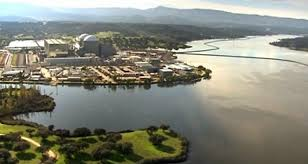
\includegraphics[width=\textwidth]{2Introduction/ArrocampoDam.jpeg}  
    \caption{\label{subfig:Arrocampo_Dam}}
    \end{subfigure}
    \hfill
    \begin{subfigure}[b]{0.45\textwidth}
    \centering
    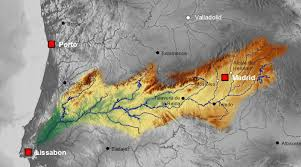
\includegraphics[width=\textwidth]{2Introduction/RioTajo.jpeg}  
    \caption{\label{subfig:TajusRiver}}
    \end{subfigure}
 \caption{a) Arrocampo dam and Almaraz Nuclear Power Plant. b) Tagus river along Spain and Portugal.}
 \label{fig:Arrocampo}
\end{figure}

Each institution of the TRITIUM collaboration is dedicated to the development of a different part of this project:

\begin{enumerate}
\item{} The University of Extremadura group has developed and installed the water purification system to produce water with very low conductivity, $\sigma \approx 10~\mu\text{S}/\cm$ (two orders of magnitude less than raw water, $1000~\mu\text{S}/\cm$). This purification process is very important for two reasons. On the one hand, for maintaining the TRITIUM detector pristine, which is critical for its long-term functionality. On the other hand, to reduce the natural background since several natural radiactive isotopes present in this water (except tritium), such as $\ce{^{40}K}$ and natural radioactive series, are removed. This system is described in section \ref{sec:UltraPureWaterSystem}.

\item{} The French group has developed the passive shielding for the detector. This shielding is made of lead with low intrinsic activity in order to reduce the external natural background of the system. This shielding is presented in section \ref{sec:IntroductionBackground}.

\item{} The Aveiro and Valencia groups have collaborated for designing, developing and building four different prototypes of the TRITIUM detector and active vetos for reducing cosmic events. These prototypes and vetos are described in chapter \ref{chap:Prototypes} and section \ref{subsec:SetUpActiveShield}, respectively. These groups have also carried out simulations of the TRITIUM monitor, which are reported in chapter \ref{chap:Simulations}.

\end{enumerate}

The important characteristics required for the TRITIUM detector are:

\begin{enumerate}

\item{} \textit{Compactness}. This is an important requirement because in the place where the detector is planned to be installed there is little space. Compactness also allows portability and cost reduction.

\item{} \textit{Modularity}. The modularity of the TRITIUM detector is important for flexible geometrical configuration and for improving its tritium detection sensitivity. Modularity also facilitates construction and maintenance.

\item{} \textit{Thin active volume and large active area}. The mean free path of $\beta$ particle from tritium decay is very short. Thus, a thin detector active volume is needed. In practice, an active thickness beyond the mean free path of the tritium electrons only contributes to background. In addition, as reported in section \ref{sec:StateOfTheArt}, the efficiency of this type of detector scales with the active area, so it is crucial to design a detector with the largest possible active area.

\item{} \textit{High detection efficiency for tritium}. As the tritium activities to be measured are very low, the loss of tritium events strongly affects the accuracy of measurements.

\item{} \textit{High specificity to tritium}. The monitor must be able to distinguish tritium signals from other radiactive decays in the sample.

\item{} \textit{Quasi-real time response}. It is crucial that the system operates in quasi-real time ($1~\hour$ or less) in order to detect any anomalous tritium release as fast as possible. 

\item{} \textit{Ruggedness}. The final goal of the project is to install an automatic system working during a number of years requiring only occasional intervention of specialized operators. Therefore, a rugged monitor is required.

\end{enumerate}

In order to measure in quasi-real time, it is needed to work \textit{in situ}, that is, in the same place where the water sample is taken. Working \textit{in situ} has some advantages such as: 1) Cheap running cost, since sampling process, chain of custody, etc. are eliminated. 2) Quasi-real time measurements. 3) Safe monitoring since personal dose is reduced. 4) Changes in activity can be detected quickly.


%In order to get the measurement in quasi-real time it is needed to work \textit{in situ}, that's, in the same place that the sample is taken. Working \textit{in situ} has some benefits:

%\begin{itemize}
%\item{} a faster monitor because we eliminates the process of taking the sample, the chain-of-custody until this sample arrive to this laboratory and the complexity which involve these tasks. 

%\item{} a better monitor since if we can work \textit{in site}, our measurements can be more frequent hence we will can identify cahnges in the activity earlier.

%\item{} a cheaper monitor because we have not only the material costs attached to the sample collection, chain-of-custody of this sample, shipping of this sample to the laboratory, etc. but we have also eliminated the costs attached to the specialized staff who are involving in these tasks. Our detector will only need frequent calibrations each time in order to ensure its correct operation.

%\item{} a safer monitor since the personal exposure dose is reduced and the changes in activity are detected fastly. On top of that we remove the possibles mistakes which can be done by specialized staff.

%\end{itemize} 
	\newpage	
	
\chapter[TRITIUM Design Principles]{Design Principles of the Tritium Monitor}\label{chap:DesignPrinciples}
	\section{Detector System Overview}\label{sec:MonitorOverview}
	The objective of the TRITIUM project is the design, development, construction and commissioning of an automatic station for real-time monitoring of low levels of tritium in water. To achieve this aim, the TRITIUM group has developed a monitor consisting of several parts, listed below: 

\begin{enumerate}

\item{} The TRITIUM detector, described in chapter \ref{chap:Prototypes}, is based on several modules read in parallel. Each module consists of hundreds of scintillating fibers, section \ref{subsec:PlasticScintillators}, which are in conectact with the water sample measured, read by two coincident photosensors, section \ref{subsec:Photosensors}. The photosensors are photomultiplier tubes (PMT) (section \ref{subsubsec:PMTs}) and silicon photomultipliers (SiPM) (section \ref{subsubsec:SiPM}).

\item{} The ultrapure water system (section \ref{sec:UltraPureWaterSystem}) that prepars the water sample before measurement. This system removes all the organic particles dissolved and all the particles with a diameter greater than $1~\mu\meter$ without affecting the tritium content of the sample. This system is important for two reasons: First, because the mean free path of tritium in water is very short, $5$ or $6~\mu\meter$,  so it is essential to avoid the deposition of particles onto the fibers because this would prevent the tritium decay electrons from reaching the fibers. Second, particles disolved in water may contains raidoactive isotopes like $\ce{^{40}K}$, which whould increase the background. As the water sample has very low tritium counters, to reduce the background is a crucial matter.

\item{} The background rejection system (section \ref{sec:IntroductionBackground}), that has two different parts. The first one is a passive shield (section \ref{subsec:SetUpPassiveShield}), consisting of a lead castle inside of which the TRITIUM detector is located. This castle is employed to eliminate natural radioactive background and cosmic rays with energies of the order of $200~\MeV/$nucleon. The second part is an active veto (section\ref{subsec:SetUpActiveShield}), consisting of two plastic scintillation blocks located inside of a passive shielding, above and below the TRITIUM detector and read by several photosensors. The goal of this active veto is to remove the remaining high energy events ($>200~\mega\eV$) cosmic rays that can travel through the passive shielding and contributo to background. Contrary to low energy cosmics rays, high energy cosmic rays are difficult to be stopped. The technique employed to eliminate their contribution consists of reading the TRITIUM detector in anti-coincidence with the active veto.
%to detect these high energy events and, for each of them, open narrow time windows in which we will not read the Tritium detector to prevent these events from affecting the tritium measurement.

\item{} A monitoring electronic system sends an alarm if the signal limit of the tritium level, $100~\becquerel/\second$, is exceeded.

\end{enumerate}

The different parts of TRITIUM monitor were subjected to tests to verify their correct operation before installing them in the Arrocampo dam. The final goal is to include TRITIUM in the network of automatic stations, REA (section \ref{sec:Introduction}). 
	%\newpage
	
	\section{TRITIUM Detector}\label{sec:TritiumDectectorIntro}
	Due to the reasons discussed in section \ref{sec:StateOfTheArt}, the TRITIUM detector developed used to measure the tritium levels of water samples is a scintillator detector. It consists in a chain of three main elements:

\begin{itemize}

\item{} The scintillator, that is the material in charge of detecting the tritium event. A general particle (tritium in our case), ionizing radiation, hit this material and deposits part of their kinetic energy (or all, as in our case) in it through ionization and excitation processes. Part of this energy deposited is converted in photons, generally in the visible range.

The produced photons produced carry information about the particle detected, such as its energy, type, etc.

\item{} The photosensor, which is the part of the detector in charge of detecting the photons produced by the scintillator that reach it (the more scintillated photons arrive to your photosensor, the better signal you have in your detector). 

The most used photosensor in nuclear physics are PMTs and SiPMs which detects the photons produced in the scintillator (with an efficiency) and transforms it in electrons which are multiplied with a factor of around $10^6$. This millions of electrons form a electronic pulse whose properties has information of the photons that has been detected.

\item{} The electronic system, which is the part of the scintillator detector in charge of processesing and analyzing (first analogically and then digitally) this electrical pulse of the photosensor. The output of the electronic system is useful information about the event detected such as a number, for instance the activity, or some kind of spectrum like energy spectrum.

\end{itemize}

In Figure \ref{fig:ScintillatorDetector} a scheme of a scintillation detector is shown. There, the scintillator material detects ionizing radiation and produces photons that will be guided by the reflector and the light guide to the photosensor. There, some of the photons that reach the sensible part of the photosensors will be converted and multiplied into millions of electrons that will form a electronic pulse. The output signal of the photosensor (electronic pulse) will be processed and analyzed by the corresponding electronics:

\begin{figure}[hbtp]
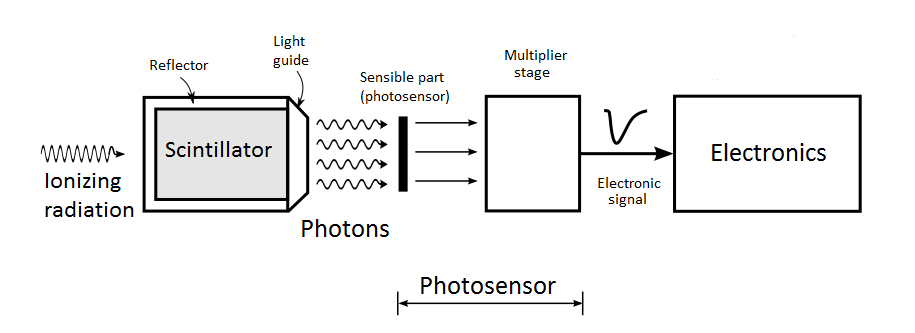
\includegraphics[scale=0.6]{3DesignPrinciples/32Tritium_detector/ScintillatorDetector.png}
\centering
\caption{Scheme of the scintillator detector\label{fig:ScintillatorDetector}}
\end{figure}
 
	%\newpage
	
		\subsection[Interaction of Particles with Matter]{Interaction of Fast Electrons and Photons with Matter}\label{subsec:Interaction}
		The interaction of particles with matter is described in this section, focusing on the particles and energy range relevant for this thesis, electrons ($0-18~\keV$), photons in the visible range (approx. $380-750~\nm$) and $\gamma$ rays from the background and high energy cosmic rays.

Electrons have a charge, so their interaction with matter is mainly through the orbital atomic  electrons by the Coulomb force. The electron trajectories are much more tortuous than those of heavier particles because of their small mass. Furthermore, electrons lose a significant amount of energy in each collision. The specific energy loss, defined as $S=-\displaystyle{\frac{dE}{dx}}$, gives the energy loss of a particle per unit of path length. In the case of electrons, the total energy loss has two main contributions, the collisions (elastic and inelastic) and the radiative processes (bremsstrahlung) which are roughly proportional \cite{Knoll, Leo},
\begin{equation}
\frac{dE}{dx} \approx \left(\frac{dE}{dx}\right)_{c} + \left(\frac{dE}{dx}\right)_{br} ; \qquad \frac{\displaystyle{\left(\frac{dE}{dx}\right)_{br}}}{\displaystyle{\left(\frac{dE}{dx}\right)_{c}}} \approx \frac{EZ}{700}
\label{eq:ElectronInteraction}
\end{equation}
where $E$ is the energy of the electron in $\MeV$ and $Z$ is the atomic number of the absorbing material. Due to this energy loss, electrons penetrate a material to a depth where they have lost their kinetic energy. This distance, known as the range, is quoted for tritium electrons in Table \ref{tab:MeanFreePathTritium}. 

The material chosen for the detection of tritium decay electrons is organic plastic since, due to its low density, there is a reduced backscattering. It has been chosen in the form of fibres in order to increase the active area and, therefore, the efficiency of the detector.

As photons do not have any charge, their possible interactions with matter are the photoelectric effect, Compton effect, coherent scattering and pair production. The probability of each process, displayed in Figure \ref{fig:ProcessesPhotons}, depends on the energy of the photon, $E_\gamma = h\nu$, and on the atomic number of the material, Z. The optical photons have a wavelength between $400$ and $700~\nano\meter$, that corresponds to energies of the order of the $\eV$. Therefore, pair production does not play any role for optical photons since this requires photon energy of at least $1.022~\MeV$.

\begin{figure}[h]
\centering
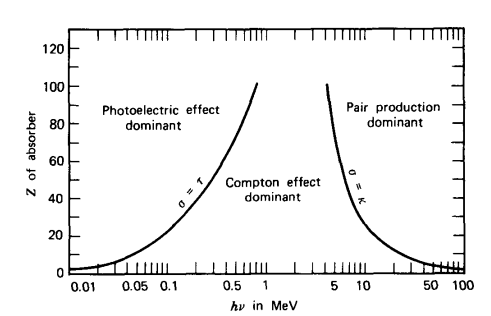
\includegraphics[scale=0.75]{3DesignPrinciples/32Tritium_detector/DominantProcessesPhotons.png}
\caption{Domain regions of the three most probable types of interactions of gamma rays with matter. The lines show the atomic number $Z$ and gamma energy $h\nu$ where two interaction processes are equally likely\label{fig:ProcessesPhotons}~\cite{Knoll}.}
\end{figure}

The photoelectric effect occurs when a photon interacts with an orbital electron in the material, losing all its energy. This energy is absorbed by an electron that is ejected from the atom (ionization). The energy of the resulting electron, $E_e$, is \cite{Knoll, Leo},
\begin{equation}
E_e = E_\gamma - E_b 
\label{eq:PhotoelectricEffect}
\end{equation}
where $E_b$ is the binding energy of the electron in the material. The probability of this effect depends on the number of available electrons in matter through the atomic number $Z$, and the energy of the electron according to the expression \cite{Knoll},
\begin{equation}
\tau \approx \frac{Z^n}{E_\gamma^{3.5}}
\label{eq:PhotoelectricProb}
\end{equation}
Thus, the photoelectric effect is most probable for elements with a high atomic number. This is the reason why these types of elements are the best shields against gamma radiation and why the passive shield of the TRITIUM monitor consists of lead bricks (section \ref{subsec:SetUpPassiveShield}). %This is also the reason why elements with high atomic number like $\ce{Sb}$ ($Z=51$), $\ce{Rb}$ ($Z=37$) or $\ce{Cs}$ ($Z=55$), are used in the cathodes of PMTs. 

The Compton effect occurs when a photon interacts with an orbital electron of the material, transferring part of its energy to the electron which is scattered at an angle $\theta$ with respect to the direction of the incident photon. If the electron binding energy is neglected, the energy transferred to it, $E_e$, is given by \cite{Knoll, Leo},
\begin{equation}
E_e=\frac{\displaystyle{\frac{E_\gamma^2}{m_0c^2}}\left(1-cos\theta\right)}{1+ \displaystyle{\frac{E_\gamma^2}{m_0c^2}}\left(1-cos\theta\right)}
\label{eq:ComptonEffect}
\end{equation}
where $m_0$ is the rest mass of the electron and $c$ is the speed of light in the vacuum. The probability of the Compton effect is proportional to the atomic number $Z$  and decreases with the energy of the photon. As it can be seen in Figure \ref{fig:ProcessesPhotons}, for photon energies in the visible spectrum (of the order of eV), the Compton effect is only likely for very light materials ($Z<4$). For heavier materials the photoelectric effect is dominant.

In the coherent scattering, the atom is neither excited nor ionized and the photon conserves its energy in the collision. Coherent scattering is probable for photons with low energies and materials with high atomic numbers. % and, as it will be shown in section \ref{subsec:PlasticScintillators}, it explains why the produced photons are guided along scintillating fibres. 

Finally, in the pair production process, the photon is converted into an electron and a positron,
\begin{equation}
\gamma \longrightarrow e^- ~ + ~ e^+
\label{eq:pairproductionprocess}
\end{equation}
As can be seen in Figure \ref{fig:ProcessesPhotons}, this is the dominant interaction process for high-energy photons, which are the photons produced by cosmic rays.


%Because of the fact that the energy of the photon doesn't change we will not speak more about this effect but it is important since this effect change de direction of photons and it will affect to their mean free path. 
		%\newpage
					
		\subsection{Plastic Scintillators} \label{subsec:PlasticScintillators}
		Scintillators are widely employed for radiation detection in nuclear physics. Scintillator converts kinetic energy of the incoming particles in to light\footnote{The light is made up of photons in the visible energy range.} which can be detected and quantified. Light emission happens through photon de-excitation of excited atoms.

Light production is linear in a wide energy range of incoming particles. Scintillators should have good optical properties, such as being transparent to the wavelenght of their own emission and having a refractive index as close as possible to that of glass for optimizing optical coupling with photosensors. Photon emission in scintillators is a stadistical process, which means that two identical events will emmit a different number of photons that follows a poisson statistics.

Scintillators can be organic and inorganic. Inorganic scintillators normally have a higher atomic number and density so their light output are higher. Due to these reasons they are better for gamma-ray spectroscopy. Organic scintillators are generally faster and they are commonly used for beta spectroscopy and neutron detection. This section is focussed on organic scintillators since they are the ones used in the TRITIUM project. 

Organic scintillators are based on a scintillator material dissolved in a base solvent, normally aromatic hydrocarbons as $\ce{C_{18}H_{14}}$, $\ce{C_{24}H_{22}N_{2}O}$ or $\ce{C_{15}H_{11}NO}$ with an average atomic numbers of which are between 3,5 and 5.

The scintillator molecules, in which the organic scintillators are based, have a $\pi$-electron structure. The energy levels of their electrons are commonly ilustrated with a Jablonsky diagram, shown in Figure \ref{fig:JablonskyDiagram}, which shows the fundamental singlet state, $S_{0i}$, where the valence electrons are, the excited singlet states, $S_{jk}$, and the excited triplet states, $T_{lm}$. The energy difference between $S_1$ and $S_0$ states is around $3$ or $4~\eV$, in the visible range. As it is shown in the figure, each energy states are splitted in close sublevels separated around $0.15~\eV$. This fine energy structure is due to excitations of molecular vibrational modes tabbed by the second index of the energy states. As the energy levels and sublevels have an energy larger than the termal energy, $0.025~\eV$, non-excited electrons are in the ground state $S_{00}$ at STP\footnote{Standar temperature and pressure conditions}.

\begin{figure}[htbp]
\centering
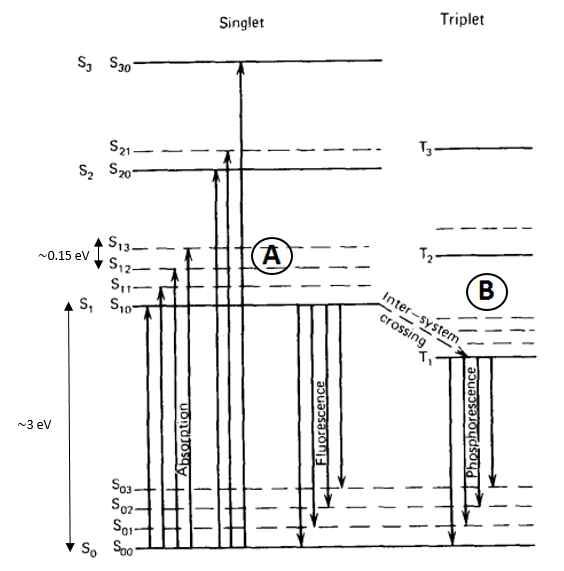
\includegraphics[scale=0.57]{3DesignPrinciples/32Tritium_detector/JablonskyDiagram.png}
\caption{Jablonsky diagram.\label{fig:JablonskyDiagram}~\cite{Knoll}}
\end{figure}

When a particle deposits their kinetic energy in a scintillator, their valence electrons are exited to higher singlet energetic states very fast (times of the order of picoseconds) and are quickly de-excited to the first singlet excited state, $S_{10}$, through non-radiative processes known as internal conversion. These electrons can de-excited to the fundamental single state, $S_{00}$, through three different physical mechanisms:

\begin{itemize}

\item{} Prompt fluorescence(process A in Figure \ref{fig:JablonskyDiagram}), where the electron in the $S_{10}$ energy level  is de-excited to some sublevel of the ground state $S_{0i}$, emitting a photon. This process happens immediately after the excitation of the scintillator molecules (around tens of nanoseconds after excitation). Each scintillator has a characteristic emission spectrum that defines its response due to the fluorescence mechanism. 

Organic scintillators are practically transparent to their own fluorescense emission because there exist a quenching effect in each de-excitation process by which all emmited  photons by the scintillator have less energy than the excitation. This effect is called Stokes shift and it is represented in Figure \ref{fig:StokesShift}.

\begin{figure}[htbp]
\centering
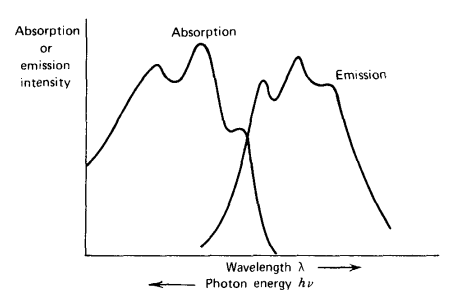
\includegraphics[scale=0.7]{3DesignPrinciples/32Tritium_detector/StokesShift.png}
\caption{Stokes shift.\label{fig:StokesShift}~\cite{Knoll}}
\end{figure}

The intensity of the fluorescence emission in an organic scintillator over time is a combination of two exponential functions, one associated with the lifetime of the level, $\tau$ (on the order of nanoseconds), and the other associated with the energetic level population, $\tau_1$ (on the order of picoseconds) \cite{Knoll}.

\begin{equation}
I=I_0\left(e^{t/\tau} - e^{t/\tau_1}\right) 
\label{eq:IntensityTimeScintillator}
\end{equation}

\item{} Phosphorescence, where the electron that is in the first single excited state cross to a triple excited state (process B in Figure \ref{fig:JablonskyDiagram}) with a process called "intersystem crossing". This is a metastable state with a longer lifetime than phosphorescence. This process happens around $10^{-3}$ seconds after scintillator excitation.

\item{} Delayed fluorescence, which occurs when an electron is in a triple excited state but its transition to the ground state is forbidden. In this case, this electron interacts with another electron in a similar state, falling and return to the first singlet state and quickly de-exciting to the ground state. 

\begin{equation}
T_{1} ~+~ T_{1}~ \longrightarrow ~ S_{1} ~+~ S_{0} ~+~ phonons
\label{eq:DelayFluorescence}
\end{equation}

This emission has the same emission spectrum as immediate fluorescence, but occurs later.
\end{itemize}

As the prompt fluorescence light produces the scintillator signal, detector design should increase it and reduce other possible physical mechanisms. One of the most important parameters is the scintillation yield\footnote{The scintillation yield is a way of expressing the efficiency of the scintillator in converting the energy deposited by the particle into photons.}, defined as the the number of photons emitted by unit of absorbed energy. This yield depends on the type of particle and on other mechanisms that doesn't produce prompt fluorescence, like phosphorescence or delayed fluorescence or even internal conversion. The scintillator yield is normally quoted by the manufacturer for mips\footnote{The MIP, Minimum Ionized Particles, is a particle that has the speed that generate minimum ionization, that's, for example, electrons with $500~\keV$ or more}.

		%\newpage
		
			%\subsubsection{Plastic scintillation fibers}\label{subsubsec:PlasticScintillatorFibers}
			Plastic scintillators are organic scintillators that has been disolved in a solven and polimerized. They are easy to machine and can take any desired shape during construction. Among the forms most used today we can find blocks, thin sheets, cylinders, etc.

In our experiment we have been working with an plastic scintillator in the form of fiber, specifically, commercial fibers BCF-12 from Saint-Gobain Crystals Inc \cite{DataSheetBCF12Fiber}. This type of fiber was chosen as the result of a comparative study \cite{TFGAlberto} among some of the best-known commercial manufacturers, such as Kuraray \cite{DataSheetKuraray}. 

The BCF-12 fibers consist of a scintillated core, whose material is polystyrene, one of the most used solvents for plastic scintillators \cite{Knoll}, with the posibility of surounding it of a cladding of polymethylmethacrylate (PMMA) (smaller refractive index than core in order to archieve a critical angle) or a multicladding (second cladding) with even smaller refractive index.

When a particle deposits all or part of its kinetic energy, some photons are produced in the fiber core as a result of the scintillating process. The number of photons produced depend on the scintillation efficiency, whose value is around $2.4\%$ for the fibers used (BCF-12), which means that $8000$ photons will be produced per $\MeV$ for a mip\footnote{The mip, minimum ionizing particle, is a particle that has the speed that generate minimum ionization.} (scintillation yield). For instance, for tritium electron, this fibers will release a maximum of around 148 photons (when tritium electron has the maximum energy, $18.6~\keV$), probably less because electrons with these energies are not mips.

These photons will shape the useful part of the response of the scintillator (fluorescence) for us. The energy (or wavelength) of these scintillated photons follows the distribution of their emission spectrum which, for the used fibers, is shown in Figure \ref{fig:EmissionSpectrumFibers}.

\begin{figure}[htbp]
\centering
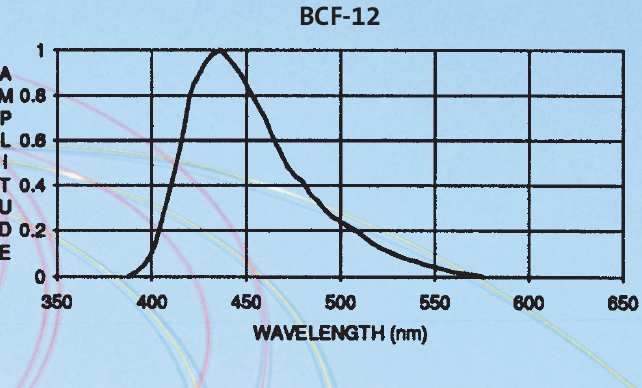
\includegraphics[scale=0.5]{3DesignPrinciples/32Tritium_detector/EmisionBCF12.png}
\caption{Emission spectrum of BCF-12 fibers of Saint-Gobain.\label{fig:EmissionSpectrumFibers}~\cite{DataSheetBCF12Fiber}}
\end{figure}

After the production of scintillated photons, we need to guide these photons to the sensitive part of the photosensor where we will detect them with some probability. Fibers (and scintillators in general) use the optical property of Snell's law \cite{Snell} to guide their photons to the desired part (the ends of the fibers). It is based on the interface created between the core and the surrounding material. When a photon hits this interface, it is refracted (and therefore lost) following the Snell equation, \ref{eq:Snell}. If the surrounding material has a lower refractive index than the core of the fiber, there exist a critical angle, $\theta_c$, at which, for angles equal or larger than this one, the photons will be totally reflected (and therefore conserved in the fiber for being guided). This effect is showed in Figure \ref{fig:Fiber_physic}.

\begin{equation}
n_0~sen(\theta_0) = n_1~sen(\theta_1) \longrightarrow \theta_c = asen\left(\frac{n_1}{n_0} \right)
\label{eq:Snell}
\end{equation}

There exist a parameter which define the efficiency of the scintillator to guide photons, the trapping efficiency or photon collection efficiency. For BCF-12 fibers with optical clad is between $3.44\%$ and $7\%$ (depending if the event was detected near the fiber axis (minimum) or near the core-clad interface(maximum)) and for no clad fibers BCF-12, it is a bit larger but presents some problems as we will see.

Therefore, from these $148$ photons initially created with the tritium electron with the maximum energy, only a maximum of around 10 photons (for maximum trapping efficiency) will arrive to our photosensor. As you can see, we work with very weak detector signals, where there is more electronic noise and, as you will see in future chapters, we have made a big effort to reduce this electronic noise as much as possible with several technics.

In Figure \ref{fig:Fiber_physic} we can see how a scintilalting fiber works.

\begin{figure}[htbp]
\centering
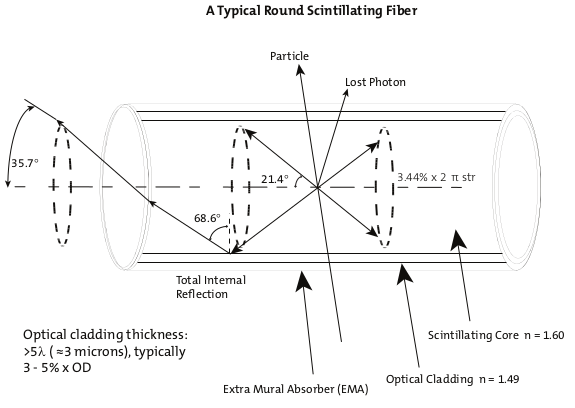
\includegraphics[scale=0.5]{3DesignPrinciples/32Tritium_detector/Fiber_data_sheet.png}
\caption{How photons are collected in a fiber with single clad.\label{fig:Fiber_physic}~\cite{DataSheetBCF12Fiber}}
\end{figure}

The cladding material is useful for protecting the core surface from dirt or aggressive external agents that can reduce the light collection but at the cost of losing some light because it increase the critical angle. In Table \ref{tab:CriticalAngles} we have three different examples where this effect is ilustrated.

\begin{table}[htbp]
%%\centering
\begin{center}
\begin{tabular}{|c|c|c|}
\hline
Material & Refractive index & critical angle ($\degree$) \\
\hline \hline \hline
Air & 1 & $42.98$ \\ \hline
Water & 1.33 & $62.47$ \\ \hline
Cladding of PMMA & 1.49 & $76.26$ \\ \hline
\end{tabular}
\caption{Critical angles asociated to different interfaces created with polystyrene, $n_0=1.6$, and other materials}
\label{tab:CriticalAngles}
\end{center}
\end{table}

This is what theoretically happens but, in the practice, it's difficult to archieve a perfect air-core or water-core interface and it will affect to the light collection. Due to the reason that the commercial claddings are thicker ($30~\micro \meter$) than the mean free path of tritium in water ( around $5~\micro\meter$) we cannot use commercial cladding in our detector hence we will need to take special attencion for archieving a water-core interface enough good. To overcome this problem, as we will see in section \ref{subsubsec:CleaningProcess}, we have used a special protocol developed in the ICMOL laboratories for preparing fibers before we use them for tritium detection.

Some of the most important parameters that descript a scintillator are summarized in Table \ref{tab:ParametersFibersBCF12} for the fibers used.

\begin{table}[htbp]
%%\centering
\begin{center}
\begin{tabular}{|c|c|c|}
%\hline
%Material & Refractive index \\
\hline \hline 
Core material & Polystyrene \\ \hline
Core refractive index & 1.60 \\ \hline
Density ($\gram/\cm^3$) & 1.05 \\ \hline
Cladding material & Acrylic (PMMA) \\ \hline
Cladding refractive index & 1.49 \\ \hline
Cladding thickness ($\mu\meter$) & 30 \\ \hline
Numerical aperture & 0.58 \\ \hline
Trapping efficiency & 3.44\% minimum \\ \hline
No. of H atoms per cc (core) & $4.82 \cdot{} 10^{22}$ \\ \hline
No. of C atoms per cc (core) & $4.85 \cdot{} 10^{22}$ \\ \hline
No. of electrons per cc (core) & $3.4 \cdot{} 10^{23}$ \\ \hline
Radiation lenght (cm) & 42 \\ \hline
Emission peak (nm) & 435 (Blue) \\ \hline
Decay Time, (ns) & 3.2 \\ \hline
1/e Length (m) & 2.7 \\ \hline
Scintillator yield (\#$\gamma$/MeV) & $\sim 8000$ \\ \hline
Operating Temperature & $-20\degree C$ to $50\degree C$ \\ \hline
\end{tabular}
\caption{Properties of BCF-12 fibers from Saint-Gobain Inc. \cite{DataSheetBCF12Fiber}}
\label{tab:ParametersFibersBCF12}
\end{center}
\end{table}

%Bunch -> manojo de fibras

%bundle -> haz de fibras%
			%\newpage
			
		\subsection{Light Detection in Photosensors}\label{subsec:Photosensors}
		The scintillating photons created in the core of the fiber and guided to its ends are detected by photosensors. Photosensors have a sensitive part that is optimized to detect photons in a range of energy (usually in the visible range) with a certain probability, called quantum efficiency. The photosensors produce an electronic signal that carries information about the detected photons such as their number, detection time, etc. There are many available photosensors that rely on various physical processes, such as photomultiplier tubes (PMTs), silicon photomultipliers (SiPM) or Charge-Coupled Devices (CCD).  %Each one of these will have different properties and it has to be chosen the one which fit better for the objective of the experiment.

The optimization of the efficiency of a scintillation detector is essential. To do so, the emission spectrum of the scintillator (Figure \ref{fig:EmissionSpectrumFibers} for the fibers used) must overlap as much as possible with the detection efficiency spectrum of the photosensor chosen. The detection efficiency spectrum of a photosensor gives the probability of detecting photons as a function of wavelength. The efficiency of a detector is proportional to the product of both, the emission and the detection efficiency spectra, and this is largest when both spectra match.

The requirements imposed on the photosensor of the TRITIUM detector are that they be very fast, have high gain and are able to detect a single photon with high photodetection efficiency. Two different porposals for the TRITIUM detector are investigated, SiPMs and PMTs. Both meet these requeriments since they are very fast (of the order of $\nano\second$), have high gain (of the order of $10^{6}$) and have a high photodetection efficiency (around $50\%$ for SiPMs and $30\%$ for PMTs). Each porposal has their own advantage. SiPMs are more robust and need a lower supply voltage (of the order of $50~\volt$) than PMTs (of the order of $1000~\volt$). Furthermore, due to this different in the supply voltage, SiPMs has a smaller cost per unit of channel than PMTs since a SiPM array, which can be feed with a single channel. However PMTs, which are the conventional choice, have lower dark count rate than SiPM a much lower dependence with the temperature.



%A certain portion (in an optimal case nearly 100\%) of the scintillation photons reach the light detector, which has to be sensitive enough to detect a small number of photons. The detector then produces a signal pulse, which has a height proportional to the number of photons hitting the detector. The signal pulse of the detector is processed by the electronics, and as a result a pulse height spectrum is produced (see Section 3.5).

%This spectrum corresponds to the energy spectrum of the detected particles.

		%\newpage
	
			\subsubsection{Photoelectron Multiplier Tubes (PMTs)}\label{subsubsec:PMTs}
			Photoelectron multiplier tube, PMT, has been employed as photosensors in nuclear physics during decades. They detect the scintillating photons that reach its sensitive part, the photocathode, and produce an electronic signal, large enough to be easily measured. In Figure \ref{fig:SchemePMT} a schematic drawing of a PMT is given. This consists of a vacuum tube that has a glass window through which photons can penetrate. The electrons created in the photocathode travel in vacuum. 

\begin{figure}[htbp]
\centering
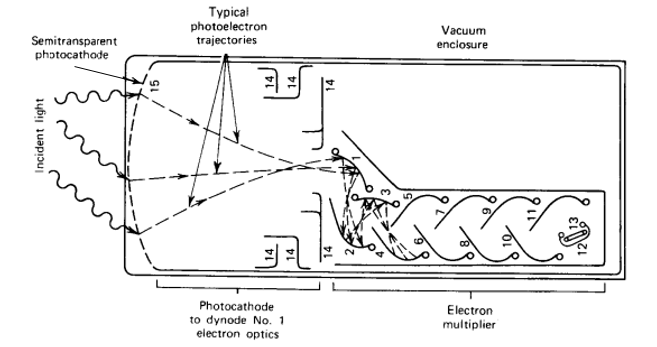
\includegraphics[scale=0.6]{3DesignPrinciples/32Tritium_detector/PMTschematic.png}
\caption{Scheme of a PMT.\label{fig:SchemePMT}~\cite{Knoll}}
\end{figure}

The signal production has two phases:
\begin{enumerate}
\item{} In the photocathode, photons are converted in photoelectrons through photoelectric effect. The photocathode consists of a thin layer, of the order of nanometers, deposited on the inner surface of the PMT window. The material of the photocathode is chosen to optimize the probability of producing photoelectric effect with the scintillating photons. The PMTs used in TRITIUM experiment are the model R8520-406 from Hammatsu \cite{DataSheetPMTs} and the material of their photocathode is Bialkali\footnote{The bialkali material is based on the elements $\ce{^{121}_{51}Sb}$, $\ce{^{85}_{37}Rb}$ and $\ce{^{132}_{55}Cs}$}.

The response of the PMT at long wavelengths is limited mainly because photon energy is not enough to produce a photoelectric effect or the emitted photoelectron does not have enough energy to overcome the material-work function. The response of the PMT at short wavelengths is limited due to absorption in the window material, quartz in our case. Thus, the response of the PMT has a strong dependence on the energy of the photon. The quantum efficiency (QE)  spectrum, shown in Figure \ref{fig:QuantumEfficiencyPMT} for the PMT used in TRITIUM, is defined as the ratio of the number of photoelectrons produced at the cathode of the PMT and the number of photons reaching it.

\begin{figure}[htbp]
\centering
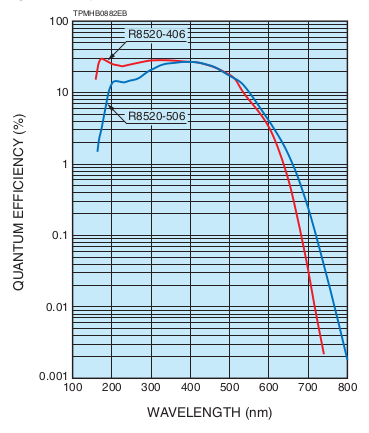
\includegraphics[scale=0.5]{3DesignPrinciples/32Tritium_detector/QuantumEfficiencyPMT.png}
\caption{Quantum efficiency spectrum for the PMT used (R8520-406).\label{fig:QuantumEfficiencyPMT}~\cite{DataSheetPMTs}}
\end{figure}

The maximum values of the PMT quantum efficiency is usually between $20\%$ and $30\%$ \cite{Knoll} (a little bit less than $30\%$ for the PMTs employed). The emission spectrum of the scintillating fibers used, Figure \ref{fig:EmissionSpectrumFibers}, matches the quantum efficiency spectrum of the PMTs used, Figure \ref{fig:QuantumEfficiencyPMT} and the position of both peaks is very close, $435~\nm$ and $420~\nm$ for fibers and PMT respectively.

\item{} As the number of photoelectrons produced in the photocatode is very small, an electron multiplication stage is employed to obtain an electronic signal of sufficient size to be processed by the electronic system. The amplification stage is based on three elements, focusing electrodes, dynodes and anode, which are metallic plates with a shape and position designed to optimize the collection and multiplication of electrons. A high voltage (HV) is applied to the PMT which is distributed between all this elements, including the photocathode, with the help of electronic circuit. A positive HV, grounded in the photocathode, is interesting for measuring PMT currents, and a negative HV, grounded in the anode, gives a faster response. The comercial electronic circuits of Hammatsu are shown in Figure \ref{fig:VoltageDividerCircuit}.

\begin{figure}[h]
\centering
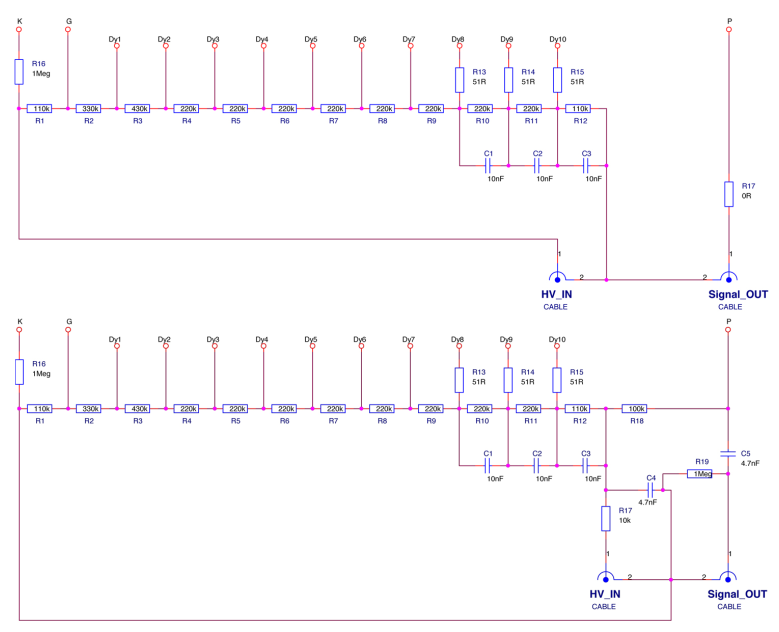
\includegraphics[scale=0.5]{3DesignPrinciples/32Tritium_detector/VoltageDividerPMT.png}
\caption{Hamamatsu commercial voltage divider electronic circuit. Upper circuit with negative supply and lower circuit with positive supply.\label{fig:VoltageDividerCircuit}~\cite{DataSheetPMTs}}
\end{figure}

%The electronic circuit that can be supplied with negative voltage is faster due to the ausence of the capacitances C4 and C5, but the other circuit, supplied with positive voltage, can be interesting for other tasks like the measurement of PMT currents. We will use both, depends on the objective of the study.

Focusing electrodes guide the photoelectrons to the first dinode. They have a collection efficiency (CE) defined as the ratio of the number of photoelectrons reaching the first dinode and the number of photoelectrons leaving the photocathode and its value is around $80\%$. The dynodes achieve the electron multiplication. A voltage difference between adjacent dynodes accelerates the electrons and produce their multiplication. The multiplication factor of each dynode, $\delta$, is commonly around 5 and is strongly dependent on the HV. If all dynodes have the same gain, the overall gain of a PMT with N dynodes is \cite{Knoll}:
\begin{equation}
G = CE\cdot{} \delta^N
\label{eq:PMTGain}
\end{equation}
that give an overall gain of a PMT of the order of $10^6$, strongly dependent on the applied HV.

The multiplication stage adds an uncertainty in the measurement. Working without gain allows to count the number of photons that reach the PMT. This can be done by short-circuiting all the dynodes and the anode and collecting the signal directly of the photocatode. This special setup was used for fiber characterization, described in section \ref{subsec:CharacterizationFibers}.

\end{enumerate}

The output pulse of a PMT has a width of the order of tens of nanoseconds. The multiplication process can be described as a Poisson statistical process. For each electron in the first dynode, G new electrons are created with a variance of $\sqrt{G}$.

The output signal of a PMT is linear with the number of photons that reach its sensitive part up to a saturation limit, at which the linearity is lost. This limit depends on the PMT model.

The photocathode may emit electrons without any scintillation light. This signal, called dark current, $I_{DC}$, can  arise due to thermoionic emission. For the PMTs used, this value is around $2~\nano\ampere$ according to their data sheet.

The characterization of the PMTs used for dark current, gain for several HV and quantum efficiency,  was done at IFIC in the framework of NEXT experiment \cite{CalibrationPMTsNEXT}. 
			%\newpageand
		
			\subsubsection{Silicon Photoelectron Multiplier Array (SiPMs array)}\label{subsubsec:SiPM}
			The Silicon Photomultiplier (SiPM) are a bind of photosensor, based on semiconductor materials, developed in recent years. They are replacing progresively conventional PMTs in many experiments and applications. They archieve outstading photon-counting capabilities with high gain and high photodetection efficiency comparing to PMT. They have conveninent characteristics as insensitiveness to magnetic fields, low operating voltage and compactness.

SiPM are based on p-n junctions, made with special techniques to archieve a good contact between both surfaces.

The voltage at which the SiPM changes from proportional to geiger mode is called the breakdown voltage, $ V_ {BR} $. At a lower voltage it works in proportional mode but at a higher voltage, it switch to Geiger mode. The measurement of the breakdown voltage is one of the most important parametes to characterize the SiPM and Its determinations is described in section \ref{sec:CharacterizationSiPM}.

The SiPM, formed by a matrix of APDs which are photodiodes operating in Geiger mode. A scheme of an APD is shown in Figure \ref{fig:SchemeAPD}. It has p+ and a n+ layers. 

\begin{figure}[htbp]
\centering
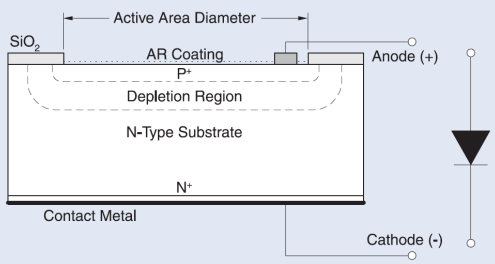
\includegraphics[scale=0.6]{3DesignPrinciples/32Tritium_detector/APD_scheme.png}
\caption{Scheme of a APD and electrical symbol used.\label{fig:SchemeAPD}~\cite{OSI}}
\end{figure}
 
These APDs, called pixels when they are part of a SiPM, are connected in parallel and the sum of all of them is read. The output signal of the pixels are quite similar regardless of the energy deposited, with some difference because of the uncertainty due to the SiPM manufacturing process and the statistical nature of the detection process. The energy deposited in each APD is not known but, as all SiPM pixels are read at the same time, the charge of the output signal when n photons are simultaneously detected is n times the charge of a sigle photon, as can be seen in Figure \ref{fig:PulsesOfSiPM}. Due to this property, after a correct calibration of SiPMs the number of detected photons we have detected is linearly related to the output signal. 

As the number of scintillating photons is proportional to the deposited energy, the linearity of its output signal and the deposited energy is obtained.

\begin{figure}[htbp]
\centering
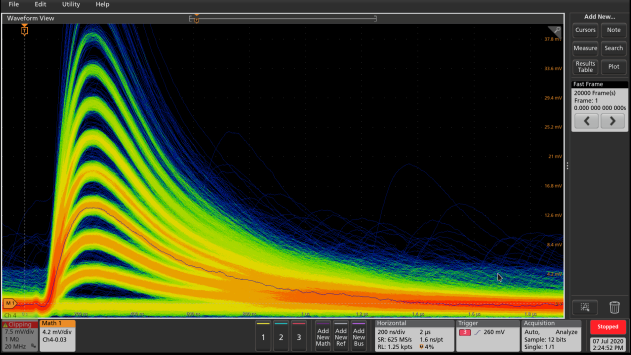
\includegraphics[scale=0.6]{3DesignPrinciples/32Tritium_detector/Several_SiPM_pulses.png}
\caption{Using persistence on the oscilloscope to show several pulses with different heights. Each height associated with a different number of  SiPM pixels lit at the same time.\label{fig:PulsesOfSiPM}}
\end{figure}

On top of that, these pixels need to be so small\footnote{Pixel sizes for commercial SiPMs are $50$ or $75\mu\meter$ \cite{DataSheetHammamatsu_1_SiPM_50}, \cite{DataSheetHammamatsu_1_SiPM_75}} that, if the photon density to be detected is low enough, we only detect one photon in each pixel. If it doesn't happen, we will detect two or more photons with the same pixel but the output signal will be the same as one detected photon, so we will have a loss of linearity of our output signal. This effect is known as saturation and it is important to know the photon density at which it happens for our SiPMs. The experimental measurements of this effect, which have been done for our SiPMs, is shown in section \ref{sec:CharacterizationSiPM}. SI LA MIDO YO PERFECTO, SI NO DECIR QUE PARA NEUSTRO CASO NO ES IMPORTANTE PORQEU ESTAMOS MIDIENDO MUY POCOS FOTONES POR EVENTO.

Each of these pixels has a quenching resistance\footnote{The tipical valuer of this quenching resistance for commercial SiPMs is around $500~\kilo\Omega$} in series that is used to stop the current produced when this pixel has detected a particle. It is used for limit the current drawn by the diode during breakdown and reduce the reverse voltage seen by the diode to one below the breakdown voltage. After that, the voltage seen by the diode is reset to the bias voltage and this pixel is ready to detect a new particle again. In Figure \ref{fig:ChenchingResistance} (left) a diagram of these chenching resistances and APDs in a SiPM and (right) how it works is shown respectively.

\begin{figure}[htbp]
\centering
{
%\subfloat[PDE]
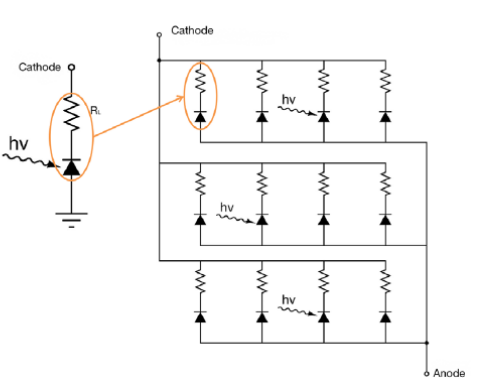
\includegraphics[scale=0.35]{3DesignPrinciples/32Tritium_detector/Quenching_resistence_of_a_SiPM_scheme.png}
%\caption{Simple electronic model of a SiPM.\label{fig:ElectricModelSiPM}~\cite{DataSheetSensL}}
}
{
%\subfloat[Espectro de emisión]
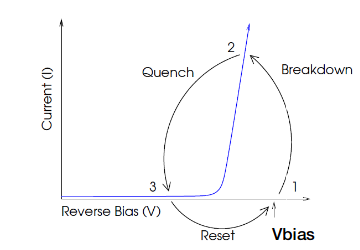
\includegraphics[scale=0.5]{3DesignPrinciples/32Tritium_detector/How_a_quenching_resistence_in_a_SiPM_works.png}
%\caption{Output current of a SiPM as a function of the reverse voltage. It show that the quenching mechanism is essential for working with SiPMs\label{fig:HowSiPMworks}~\cite{DataSheetSensL}}
}
\caption{(Left) Electronic scheme of a SiPM and (right) output current of a SiPM as a function of the reverse voltage. It show that the quenching mechanism is essential for working with SiPMs\label{fig:ChenchingResistance}~\cite{DataSheetSensL}}
\end{figure}

In this simple electrical scheme we can see that all pixels have a common cathode and anode which means that, as we said before, they are at the same bias voltage and the output is the sum of all of them.

We have a lot of names to refer to these photosensors such as SiPMs, MPPCs, G-APDs, SSPMs, MRS-ADPs or AMPDs. The candidate for TRITIUM project is S13360-6075 from Hamamatsu photonics \cite{DataSheetHammamatsu_1_SiPM_75} because its characteristics are the ones that best fit our objectives since this model has super low afterpulses, crosstalk and dark counts than other SiPM models from Hamamatsu. Its characteristics and properties are shown in Table \ref{tab:PropertiesOfSiPM75}. 

\begin{table}[htbp]
%%\centering.
\begin{center}
\begin{tabular}{|c|c|}
\hline
Parameter & Numerical value \\
\hline \hline \hline
Serie & $S13360$ \\ \hline
Model & $6075$ \\ \hline
Pixel Pitch ($\mu\meter$) & $75$ \\ \hline
Effective photosensitive area ($\mm^2$) & $6.0 \times 6.0$ \\ \hline
Number of pixels & $6400$ \\ \hline
Fill factor & $82\%$ \\ \hline
Refractive index of windows material & $1.55$ \\ \hline
Operating temperature range ($\degree C$)& $[-20,60]$ \\ \hline
Spectral response range, $\lambda$ ($\nano\meter$) & $[320, 900]$ \\ \hline
Peak sensitivity wavelength, $\lambda_p$ ($\nano\meter$) & $450$ \\ \hline
PhotoDetection Efficiency, PDE, $\lambda=\lambda_p$ ($\%$) & $50$ \\ \hline
Dark counts, Typical/Maximum (kcps) & $2000/6000$ \\ \hline
Terminal capacitance, $C_t$ ($\pico\farad$) & $1280$ \\ \hline
Gain, M, & $4 \cdot{} 10^6$ \\ \hline
Breakdown Voltage, $V_{BR}$ ($\volt$) & $53$ \\ \hline
Cross talk probability($\%$) & $7$ \\ \hline
Temperature coefficient $\Delta TV_{op}$ (m$\volt/\degree C$) & $54$ \\ \hline
\end{tabular}
\caption{Characteristics of SiPM S13360-6075 from Hamamatsu Photonics \cite{DataSheetHammamatsu_1_SiPM_75}.}
\label{tab:PropertiesOfSiPM75}
\end{center}
\end{table}

These characteristics and properties will be explained and their experimental measurements will be shown in section \ref{sec:CharacterizationSiPM}. These numerical values, which appear in Table \ref{tab:PropertiesOfSiPM75}, are provided by Hamamatsu photonics but it is only an approximation for this model. These parameters must be determined experimentally for each SiPM used because it can be very different even if it is the same model.

It must be taken into account that we will do this characterization at the level of a single SiPM because, at the beginning, it is easier to understand the results but we will work with a matrix of them and we will have to do this characterization for each matrix used. 

The matrices under consideration are the model "S13361-6050" from Hamamatsu, which consists of a $4\times 4$ SiPM matrix where the active area of each SiPM is $6\times 6~\mm$ \cite{DataSheetHammamatsu_array_SiPM_6050} or the model "S13361-3050" from Hamamatsu, which consists of a $8\times 8$ SiPM where the active area of each is $3\times 3~\mm$ \cite{DataSheetHammamatsu_array_SiPM_3050}. They are a commercial matrices from Hamamatsu and, as you can see, the total active area that we will cover with these arrangements is the same in both cases, $24\times 24~\mm$ and it is approximatelly the same that the active area covered with the PMTs used, which has been shown in the previous section.

These matrices have a common bias voltage and common ground for all SiPMs that are contained and we will have an output signal for each SiPM. 

We hope to obtain better results with the 4x4 matrix for theoretical reasons which we will see in section \ref{sec:CharacterizationSiPM} like larger PDE, mainly due to a larger active area but it is something that we will have to verify with experimental measurements.




Nuestro SiPM esta dopado? con que?
			%\newpage
			
			\subsubsection[Comparison Photosensors]{Comparison of photosensors considered}\label{subsubsec:ComparisonPhotosensors}
			The photosensors employed in TRITIUM are both, PMT and SiPM. Each kind of photosensor has its advantages and disadvantages, so both were tested to decide the most suitable. The output signal of both photosensors is proportional to the number of incident photons in our range of luminosity and they have a similar gain (of the order of $10^6$). Both properties are essential to detect tritium events and to obtain a large enough signal to be measured and recorded. Both photosensors have fast output signals, with a rise time of the order of nanoseconds, and a wide spectral sensitivity ($200-800~\nano\second$ for PMT and $300-900~\nano\second$ for SiPM). The supply voltage necessary to work with SiPM, of the order of tens of volts, is much lower than that of PMTs, which require a high voltage, of the order of a thousand volts. The electron detection efficiency at $420~\nano\meter$,  achieved with SiPM is higher, PDE around $50\%$, than with PMT, which have a QE about $30\%$. A large efficiency is essential because the number of photons produced in a tritium event is rather low. Furthermore PMTs, as they consist of a vacuum tube, are more bulky and fragile than SiPMs, which are compact and robust. This is an advantage for the SiPMs because the TRITIUM detector should work during years. Furthermore, PMTs are rather more expensive, than SiPMs. In addition, PMTs are affected by magnetic fields, contrary to SiPMs that work correctly in magnetic field up to 7 Tesla. Moreover, due to their high uniformity, SiPMs are capable of measuring the exact number of photoelectrons detected and even of resolving a single photoelectron, which is not possible with PMTs due to their gain uncertainty.

However, the dark current of PMTs is much lower (a few counts per second) than that of SiPMs, that have a dark current between 0.1 and 1 Mcps\footnote{Mega counts per second, $10^6$c/$\second$}, depending on their size, and this happens with SiPMs almost entirely at the level of a single photoelectron. This prevents to separate tritium decay signals from background in the singel photon-detection zone. Another inconvenient of SiPMs is their large crosstalk and afterpulses that need to be corrected. An additional drawback of SiPMs is that their response depends strongly on temperature. As the TRITIUM detector will be installed in an environment with significant temperature variations, this problem is solved by developing a stabilization method of the SiPM gain.
			%\newpage
					
		\subsection{Electronic Readout}\label{subsec:IntroductionElectronicalSystem}
			The electronic system is in charge of reading, processing and analyzing the output signal of photosensors and providing output information about tritium detection. This electronic system depends on the type of output information that is desired and on the detector configuration used.

%In each type of detector configuration, this electronic system will also be different depending on the type of information we want to obtain. For example, it will be different if we want to obtain an energy spectrum as output information or simply a number such as the number of counts per second of our detector or the output electrical current. Each electron system that has been used in our experiment will be explained during this section.

 
			%\newpage
	
			\subsubsection[Electronic Readout for PMTs]{Electronics for PMTs}\label{subsubsec:PMTsElectronicalSystem}
			PMTs were used in TRITIUM experiment for two main objectives. On the one hand, to determine the amount of incident photons that reach the PMT photocathode, which is important to characterize fibers, and, on the other hand, to measure the energy of events, which allows us to discriminate events according to their origin, obtaining an energy spectrum of tritium events in water from laboratory prototypes.

To know the amount of photons that reach the photocathode, as explained above, the PMT should work without internal gain since it introduces a large uncertainty in the measurement. For that end, the homemade electron multiplication stage of Figure \ref{fig:ElectronicSchemeBasePMTNoGain} is employed. 

As the electrons are not multiplied, the output pulse of the photosensor is very small (currents of the order of tens of nanoamperes) and a special readout system is needed. The chosen system is Keithley 6487 Picoammeter/Voltage Source \cite{DataSheetKeithley6487}, a commercial system from Keithley. This system has some useful options such as automatic baseline correction, the ability to read currents of the order of picoamperes and the possibility of carrying out mathematical operation on the signal, such as the average of N measurements with the associated statistical error, where N is programmable by the user ($N=100$ in all our studies). 

To determine the energy of the events, the gain of the PMT has to be restored by removing the short-circuit of the electron multiplication stage. The number of PMTs used simultaneously was one, two or four, depending on the setup. A simplified scheme of the electronic chain employed in each case is shown in Figures \ref{subfig:ElectronicConfiguraiton1PMT}, \ref{subfig:ElectronicConfiguraiton2PMT} and \ref{subfig:ElectronicConfiguraiton4PMT}, based on various NIM modules\footnote{The Nuclear Instrumentation Module (NIM) is a standard specification convention for electrical and mechanical parameters defined in electronic modules used in experimental nuclear and particle physics.}.

\begin{figure}
\centering
    \begin{subfigure}[b]{1.0\textwidth}
    \centering
    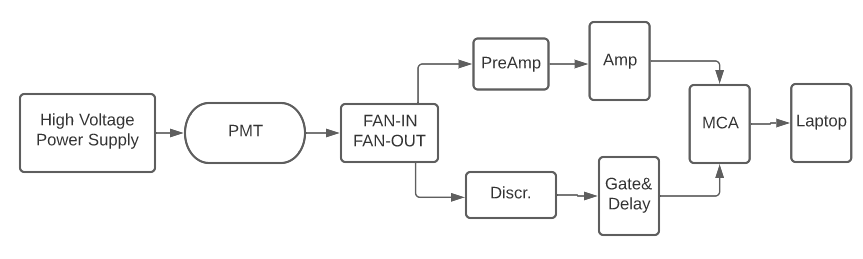
\includegraphics[width=\textwidth]{3DesignPrinciples/32Tritium_detector/Electronical_Scheme_1_PMT.png}  
    \caption{\label{subfig:ElectronicConfiguraiton1PMT}}
    \end{subfigure}
    \hfill
    \begin{subfigure}[b]{1.0\textwidth}
    \centering
    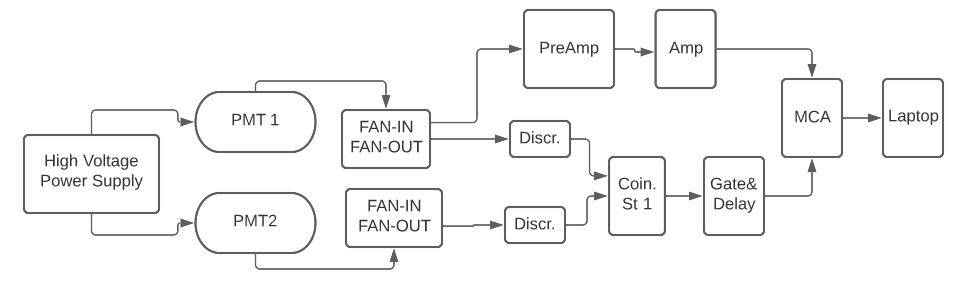
\includegraphics[width=\textwidth]{3DesignPrinciples/32Tritium_detector/Electronical_Scheme_2_PMTs.png}  
    \caption{\label{subfig:ElectronicConfiguraiton2PMT}}
    \end{subfigure}
    \hfill
    \begin{subfigure}[b]{1.0\textwidth}
    \centering
    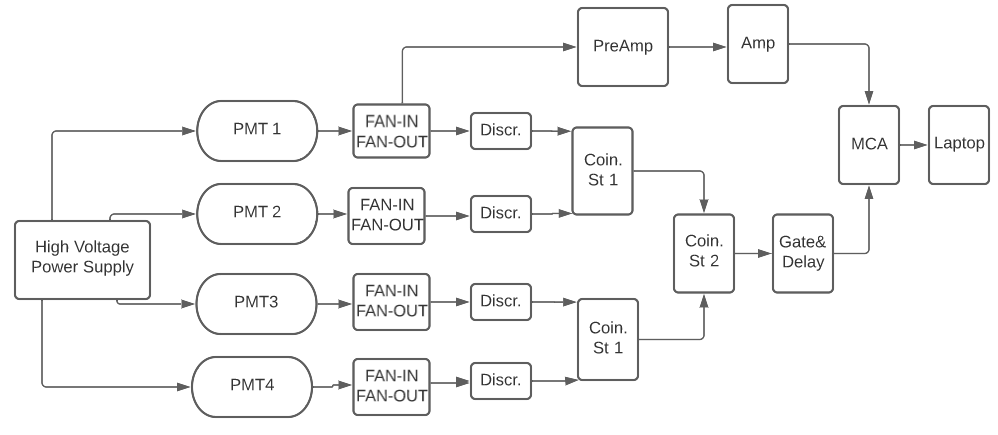
\includegraphics[width=\textwidth]{3DesignPrinciples/32Tritium_detector/Electronical_Scheme_4_PMTs.png}  
    \caption{\label{subfig:ElectronicConfiguraiton4PMT}}
    \end{subfigure}
 \caption{Schemes of the different electronic for measuring with PMTs. a) Employed when only one PMT is used. b) Employed when two PMTs are used in time coincidence. c) Employed when four PMTs are used in time coincidence.}
 \label{fig:ElectronicConfiguraitonsPMT}
\end{figure}

The PMTs were biased in all the cases by TC 952 High Voltage Supply from Tennelec \cite{DataSheetHVSupplyTennelec}, which has four channels. If two or more configurations are needed, a second voltage supply HV Power Supply N 1130-4 from Wenzel Elektronik company \cite{DataSheetHVSupplyWenzel} with 4 additional channels, was employed. As it can be seen in the figures, there are two different lines followed by the PMT output signals, the amplification line, used to create an energy spectrum, and the time coincidence line, used to make time coincidences. Therefore, an analogic FAN IN-OUT module was used to duplicate the input signal. The module employed was the Quad linear FAN IN-OUT MODEL 740 from Philips Scintific \cite{DataSheetFANINOUT}, which has four channels. One output signal was used as the input for the amplification part and the second output was used as input for the time coincidence electronics.

\begin{enumerate}

\item{} The amplification line, which is the same for the three configurations, provides the energy information and is based on two steps;

%We have to take into accout that we have only used the signal from one PMT for the amplification part. We could have added a stage where we add the four PMT output signals and it would probably improve our results, but since our ultimate goal is to work with SiPM, we have not delved into that.

%The electronic path we have followed to achieve this amplification is:

\begin{enumerate}

\item{} The output signal is integrated by a preamplifier, which gives an output signal with a heigth proportional to the charge of the input pulse. This signal has a long tail\footnote{The length of the tail is, $\tau=RC$, where R is the input resistance and C is the capacitance used. It is the typical output signal in RC circuits.} produced by the preamplifier capacitance. The preamplifier used was "MODEL 9326 FAST PREAMP" from ORTEC \cite{DataSheetPreAmp}.

\item{} The output signal from the preamplifier is lead to the amplifier which gives a gaussian shaped output signal. The amplifier modules were 575A and 671 from ORTEC \cite{DataSheet575Amp, DataSheet671Amp}. An example of the output signal for 575A module is shown in Figure \ref{fig:InputSignalsMCA}, green color.

\end{enumerate}

\item{} The time coincidence line contains the time information and gives the gate that triggers coincident signals of both PMTs. This line consists of the following branches,

\begin{enumerate}

\item{} The output signal of the FAN IN-OUT module of each PMT is introduced into a discriminator module that gives a logic signal of $-1.2~\volt$ height and of $240~\nano\second$ width when a given threshold is exceeded. The discriminators employed are  Octuple Constant-Fraction Discriminator CF8000 module from ORTEC \cite{DataSheetDiscriminator} and 4 channels discriminator model 84 from CAEN \cite{DataSheetDiscriminatorCAEN}.

\item{} Time coincidences are required to ensure that detected events come from the scintillating fibers and to remove external light and dark current. The two logic signals given by the discriminator from the two PMTs that read a detector are introduced in a coincidence module which generates an output signal of $-1.4~\volt$ heigh and of $20~\ns$ width, when both imputs are in time coincidence. The modules used were Coincidence Unit Model 465 from LeCroy \cite{DataSheetCoincidenceLeCroy} and Coincidence Type N6234 from CERN-NP \cite{DataSheetCoincidenceCERN}.

\item{} Time coincidence of two different detectors (4 PMTs, configuration \ref{subfig:ElectronicConfiguraiton4PMT}) was also studied, which is useful to remove background due to hard cosmic radiation. To do so, a coincidence step similar to the previous one must be applied. The two single detector coincidence signal are checked for coincidence.

Some examples are shown in Figure \ref{fig:DifferentCoincidences} for time coincidences of two detectors (4 PMTs). There, four logical signals are shown, two of them (channel one and two, yellow and green respectively) come from two PMTs reading the first detector and the other two signals (channels three and four, color orange and violet respectively) come from PMTs reading the second detector.

\begin{enumerate}
\item{} In Figure \ref{subfig:signalInOnePMT} only one PMT (channel two) detected an event. It means that the event is likely not produecd in the scintillator. In this case, no output signal is generated.

\item{} In Figures \ref{subfig:signalInTwoPMTOneDetector} and \ref{subfig:signalInTwoPMTOtherDetector} two PMT signals of on of the detectors are generated but the other detector gives no signal. This event is discarded.

\item{} In Figure \ref{subfig:signalInAllPMTsBothDetector} the four signals are generated and, consequently, the output signal is generated and the event is recorded.

\begin{figure}
\centering
    \begin{subfigure}[b]{0.45\textwidth}
    \centering
    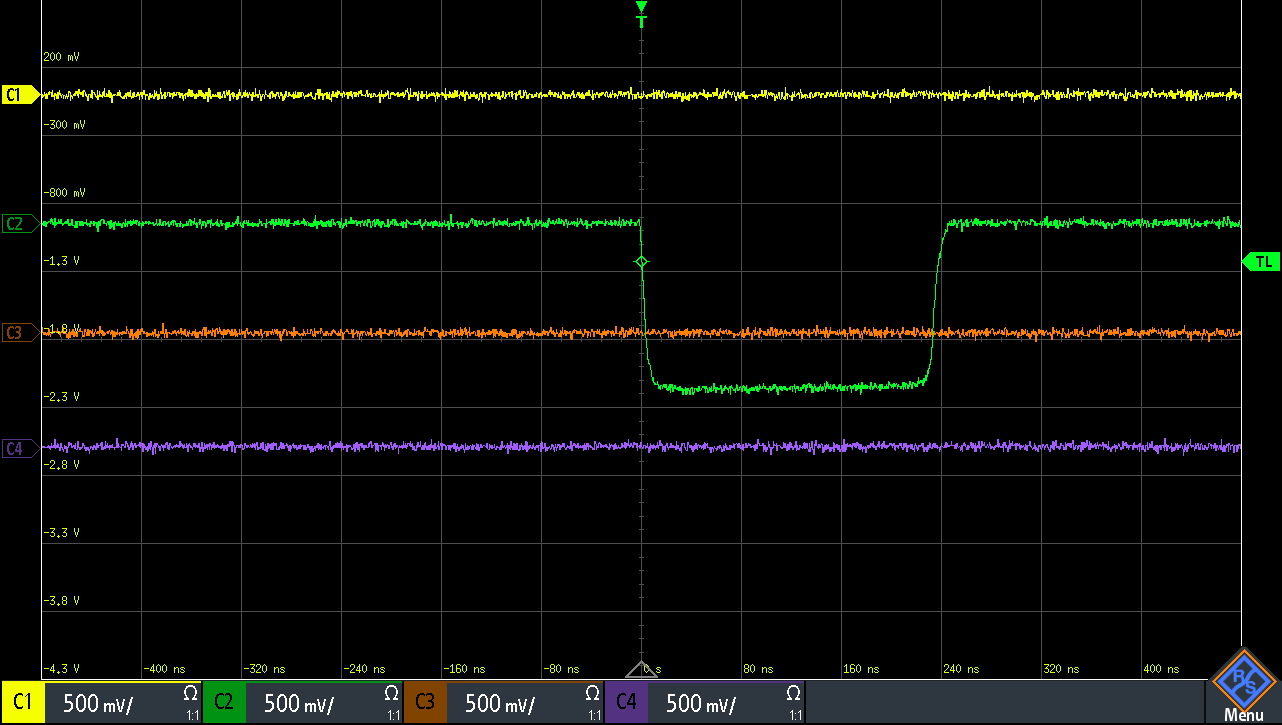
\includegraphics[width=\textwidth]{3DesignPrinciples/32Tritium_detector/1_coincidences.png}  
    \caption{\label{subfig:signalInOnePMT}}
    \end{subfigure}
    \hfill
    \begin{subfigure}[b]{0.45\textwidth}
    \centering
    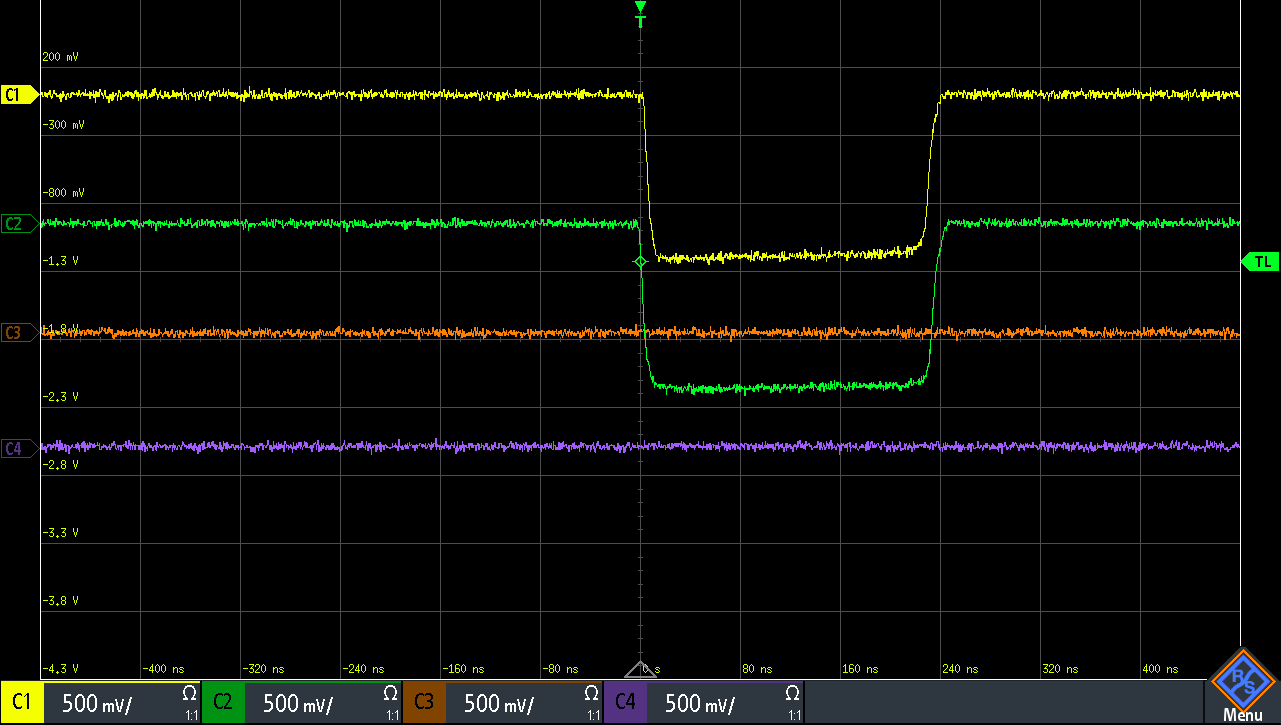
\includegraphics[width=\textwidth]{3DesignPrinciples/32Tritium_detector/2_coincidences_1.png}  
    \caption{\label{subfig:signalInTwoPMTOneDetector}}
    \end{subfigure}
    \hfill
    \begin{subfigure}[b]{0.45\textwidth}
    \centering
    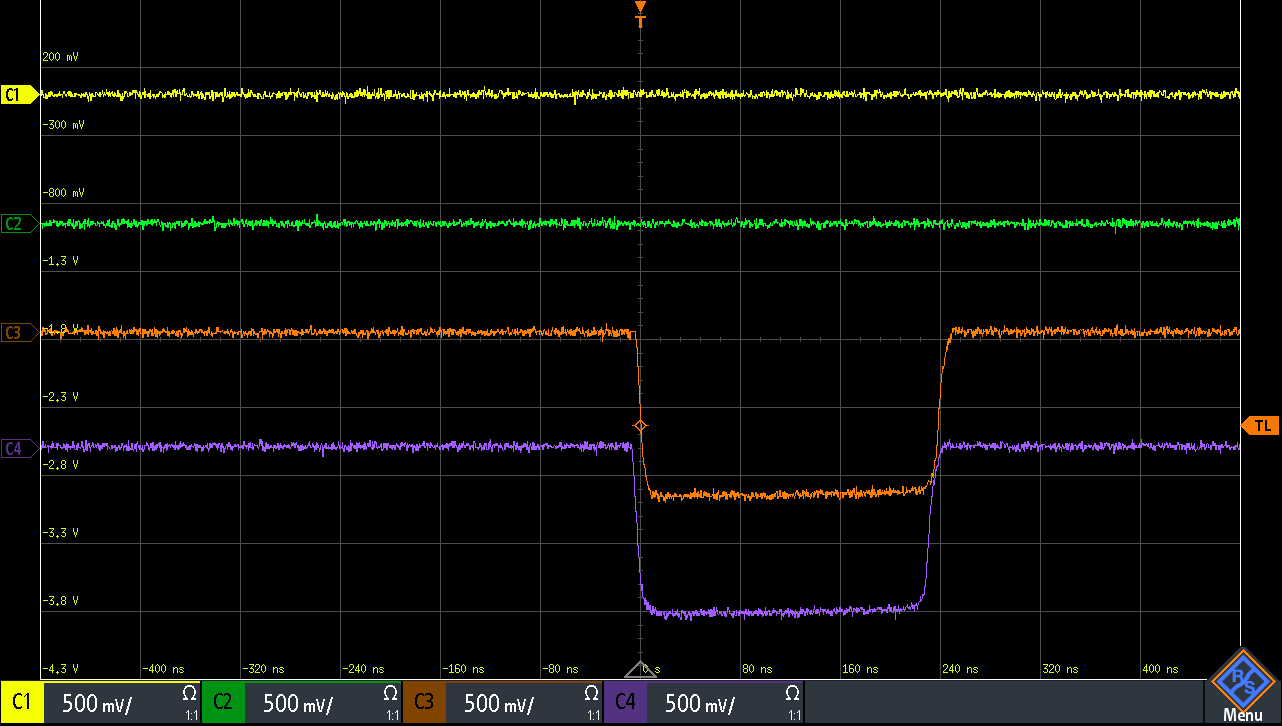
\includegraphics[width=\textwidth]{3DesignPrinciples/32Tritium_detector/2_coincidences_2.png}  
    \caption{\label{subfig:signalInTwoPMTOtherDetector}}
    \end{subfigure}
    \hfill
    \begin{subfigure}[b]{0.45\textwidth}
    \centering
    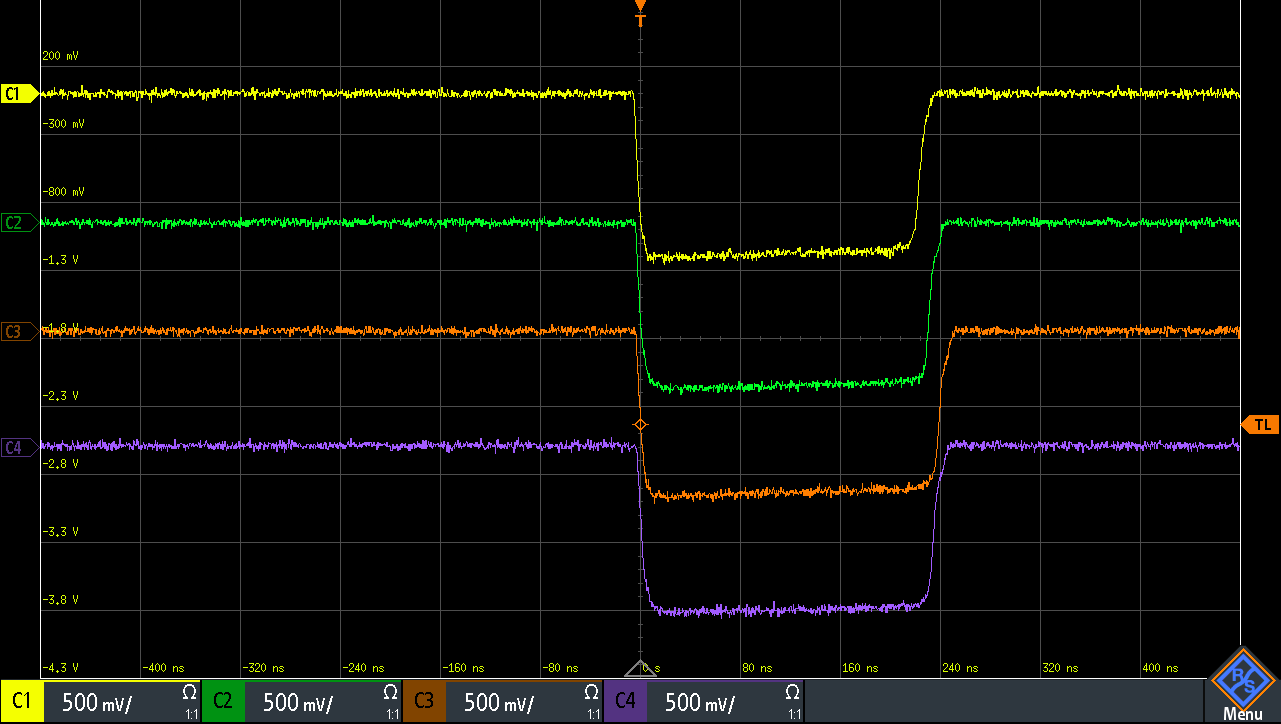
\includegraphics[width=\textwidth]{3DesignPrinciples/32Tritium_detector/4_coincidences.png}  
    \caption{\label{subfig:signalInAllPMTsBothDetector}}
    \end{subfigure}
 \caption{Different possibilities when time coincidences with PMTs are done. a) Event detected in only one PMT, one detector. b) Event detected in two PMTs, one detector. c) Event detected in two PMTs, other detector. d) Event detected in all PMTs, both detector.}
 \label{fig:DifferentCoincidences}
\end{figure}

\end{enumerate}

\item{} The logical output signal, is introduced in the Gate and Delay Generator, model 416A of the company ORTEC \cite{DataSheetGateAndDelay}, which gives a positive logical signal, called time windows, shown in Figure \ref{fig:InputSignalsMCA}, orange color, with a height of $8~\volt$ and width of $2~\mu\second$. This module is used to delay the time windows until it overlaps with the energy signal as it is shown in Figure \ref{fig:InputSignalsMCA}, orange signal.

\end{enumerate}

\end{enumerate}

As a final output of the electronics, a logical and analogical signals are obtained, shown in Figure \ref{fig:InputSignalsMCA}, which are recorded by the MCA 8000D, Pocket MCA from AMPTEK \cite{DataSheetMCA}. The analogical signal has information about the energy of the event and this is the signal which information is saved for later analysis. The logic signal (output from the Gate and Delay Generator module) indicates when the amplified signal must be saved.

\begin{figure}[htbp]
\centering
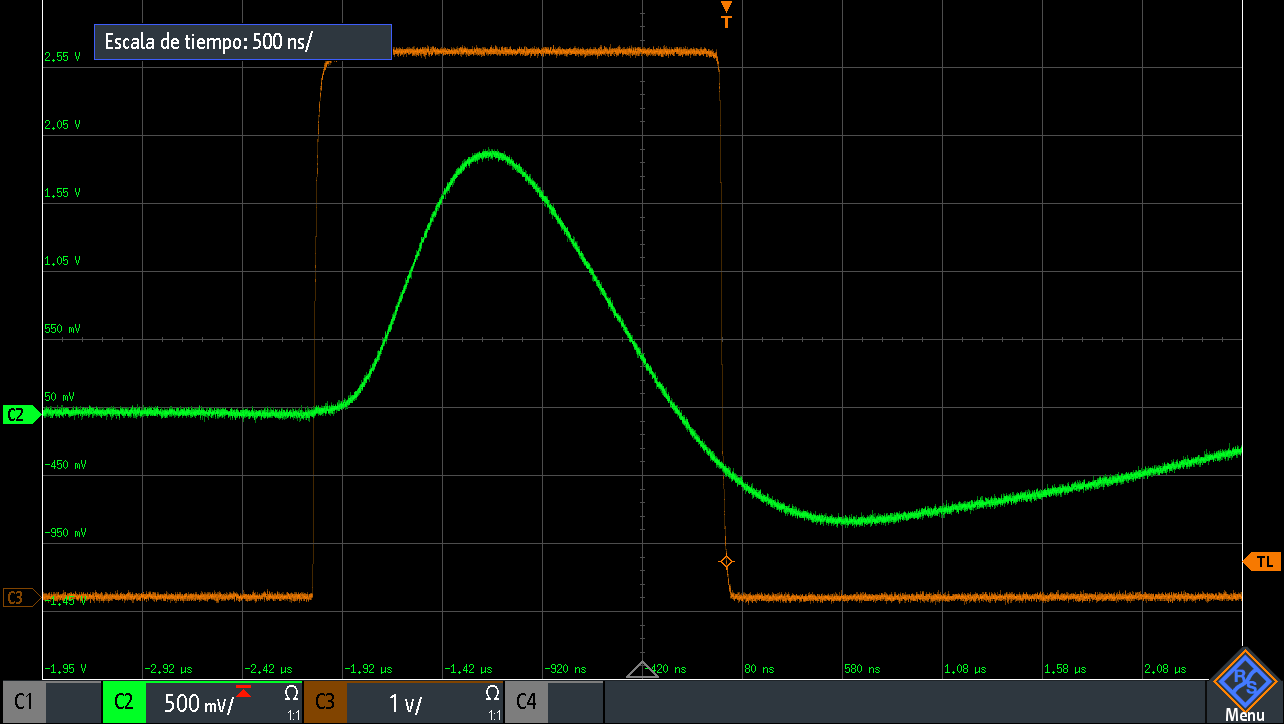
\includegraphics[scale=0.3]{3DesignPrinciples/32Tritium_detector/Input_MCA.png}
\caption{Signal amplified and logical gate (input signals of MCA).\label{fig:InputSignalsMCA}}
\end{figure}
			%\newpage
			
			\subsubsection[Electronic Readout for SiPMs]{Electronical system for SiPMs}\label{subsubsec:SiPMsElectronicalSystem}
			The SiPMs in the TRITIUM experiment are arranged in matrices of $4\times 4$. The electronic system chosen to process and analyze the output signals of the SiPM arrays is PETsys \cite{PETSYS}, displayed in Figure \ref{fig:PETSYS}, which is a commercial system prepared to work with SiPM matrices from Hamamatsu. PETsys provides time and energy digitalization, including the charge integrations QDCs\footnote{charge-to-digital converter} and TDCs\footnote{time-to-digital converter}, resulting in a complete acquisition and digitization system capable of working with up to 1024 SiPM. This system consists of a basic board to which 16 different SiPM matrices can be connected with up to 64 SiPM per matrix. This number of channels is needed in the TRITIUM project because, as shown in section \ref{sec:TritiumMonitor}, the TRITIUM monitor consists of a large number of SiPM matrices with 16 channels per matrix.

\begin{figure}[h]
\centering
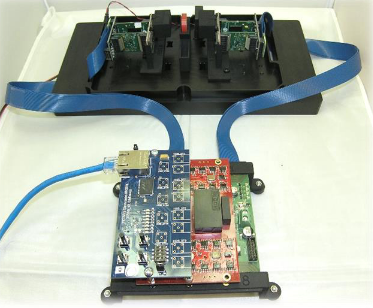
\includegraphics[scale=0.8]{3DesignPrinciples/32Tritium_detector/PETSYS_System.png}
\caption{Different parts of PETsys system\label{fig:PETSYS}~\cite{PETSYS}.}
\end{figure}
Although the capacity provided by PETsys should be enough for the requirements of the TRITIUM project, TRITIUM is a modular detector with scalable sensitivity. This means that, if an inprovement of TRITIUM limits is needed to improve its sensitivity or to further reduce the background, more photosensors would be needed. Therefore, the electronics should be able to increase its capacity in a scalable way. This requeriment is fulfilled by PETsys since it has an additional module, called Clock and Trigger, to which up to sixteen different PETsys basic boards can be connected. Theses sixteen PETsys basic boards are read in parallel, giving a total system capacity of reading 256 SiPM matrices (16384 SiPMs\footnote{$1024\cdot{}16 = 16384$}). 

PETsys software is based on C++ and Python scripts to drive the main tasks required, such as time coincidence options between SiPM (or even SiPM matrices) or energy discrimination. This software is open source, giving the possibility to modify the current scripts or to develop others with additional functions. PETsys has a time resolution better than $30~\pico\second$ which is one of the best time resolutions of commercial systems available and its price is around $10$\euro$/$ channel, which is cheaper than similar electronic systems.

As reported in section \ref{sec:CharacterizationSiPM}, the SiPM matrix temperature is an important parameter. The PETsys system has the ability to monitor the temperature of the SiPM matrices and ASICS employed to control them. Temperature monitoring is important to ensure the correct functioning of both photosensors and system. PETsys has the possibility of developing new scripts to implement the stabilization method of the SiPM gain reported in section \ref{sec:CharacterizationSiPM}.

Some characterization measurements were carried out using the PETsys system to ensure that the system works properly but the SiPM characterization was carried out at the level of a single channel (individual SiPM). The reason is that the output information of PETsys is already integrated and digitized, so it does not allow the SiPM to be calibrated. Therefore, to characterize a SiPM, a different electronic system was used to read up to eight different SiPMs. This system consists of a PCB that provides the SiPM bias voltage and reads the SiPM output signal. An example of the electronic scheme (provided by Hamamatsu) in which this PCB is based is shown in Figure \ref{fig:PCBSiPM}.

\begin{figure}
\centering
    \begin{subfigure}[b]{0.5\textwidth}
    \centering
    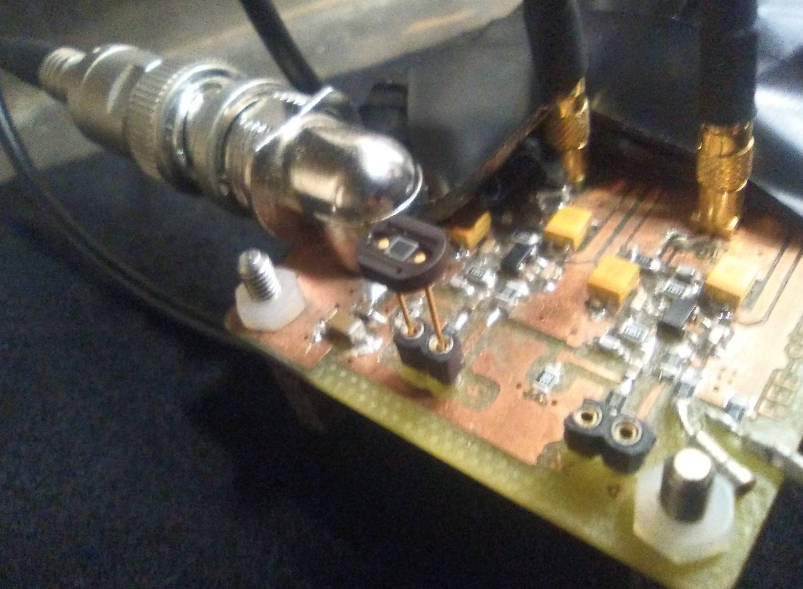
\includegraphics[width=\textwidth]{3DesignPrinciples/32Tritium_detector/SiPMPCB.png}  
    \caption{\label{subfig:ElectronicBoardSiPM}}
    \end{subfigure}
    \hfill
    \begin{subfigure}[b]{0.45\textwidth}
    \centering
    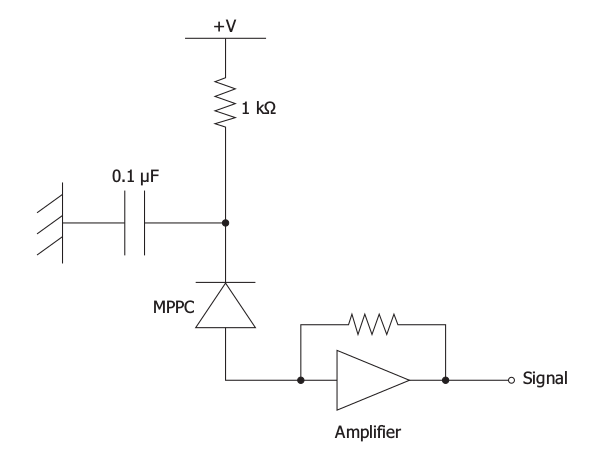
\includegraphics[width=\textwidth]{3DesignPrinciples/32Tritium_detector/ElectronicSchemePCBSiPM.png}  
    \caption{\label{subfig:ElectronicSchemePCBSiPM}}
    \end{subfigure}
    \hfill
 \caption{a) Electronic board used to provide the SiPM bias voltage and to read the SiPM output signal. b) Electronical scheme in which this PCB is based.}
 \label{fig:PCBSiPM}
\end{figure}
The PCB was feed at $\pm6~\volt$ using the voltage source ISOTECH, model IPS-4303 \cite{VoltageSourceISOTECH} and the SiPM was feed using the electrometer KETHLEY, model 6517B \cite{VoltageSourceKethley}, that achieves a resolution of $1~\milli\volt$, low enough to ensure that this voltage variations does not affect the SiPM gain. The output signal of this PCB is connected to an oscilloscope, model WwaveRunner 625Zi from TELEDYNE LECROY \cite{OscilloscopeIFIMED} that records the data which were subsequently analized by ROOT\footnote{ROOT is a framework for data processing, based on C ++ and object-oriented technology, developed at CERN and widely used in nuclear and particle physics.} scripts.
			%\newpage		
		
	\section{Ultrapure Water System}\label{sec:UltraPureWaterSystem}
	%\input{./Sections/3Design_Principles/33UltraPureWaterSystem} 
	%\newpage
		
		\subsection[Introduction to the Water System]{Introduction to the Ultrapure Water System}\label{subsec:IntroductionWaterSystem}
		The water samples, which will be introduced into the TRITIUM detector to be measured, are taken directly from the Tajus river, 4 km downstream from the place where the Almaraz Nuclear Power Plant releases the cooling water. This sample, as it was verified by a detailed analysis shown in section \ref{sec:CharacterizationUltraPureWaterSystem}, contains many dissolved elements such as minerals, organic deposits, and living matter dissolved in the water. These dissolved items need to be deleted for several reasons:

\begin{enumerate}

\item{} The mean free path of tritium electrons in water is around $5~\mu\meter$ and even less in solid materials like organic material. Tritium decay electrons have to reach the fiber to be detected and, consequently, the detector must be kept very clean. If the analyzed water sample contains particles that may be deposited on the fibers, a layer of matter could be formed, preventing tritium decay electrons from reaching the fibers and reducing drastically the tritium detection efficiency.

\item{} The tritium monitor does not have any spectrometric capabilities that could be used to distinguish tritium from other radioactive elements from minerals dissolved in the water.

\end{enumerate}

The water purification system was designed to remove organic matter and mineral particles with a size of up to $1~\mu\meter$. Hence, this filtering should keep unchanged the tritium level in the water. 

%Since tritium is the only radioactive element that can be practically equal to water (when it is in the $\ce{HTO}$ form, the majority form in wihch tritium are present in the water sample), with this process we remove all particles radioactive elements other than tritium and the amount of tritium present in the sample is not affected



%In summary, the ultrapure water system is used to keep our detector clean, ensuring the stability of its detection efficiency and to eliminate all radioactive particles other than tritium. %maintaining the activity of the tritium in the sample. Both reasons has been tested with experimental measurements, shown in secton \ref{sec:CharacterizationUltraPureWaterSystem}. 
		%\newpage
					
		\subsection[Water System Design]{Design of the Ultrapure Water System}\label{subsec:SetUpWaterSystem}
		The requeriments of this water treatment device are:

\begin{itemize}

\item{} to obtain a high degree of purification of the processed water sample, reducing its conductivity by approximately two orders of magnitude (from $1000~\mu$S$/\cm$ to $10~\mu$S$/\cm$)

\item{} to require of low maintenance (low cost  and low manpower)

\item{} to install a remote control device with probes and valves contolling by software.
\end{itemize}

The LARUEX laboratory in Extremadura, one of the six collaborators of the TRITIUM experiment, has designed, developed and built the ultrapure water system, a scheme of which is shown in Figure \ref{fig:WPSScheme}.

\begin{figure}[htbp]
\centering
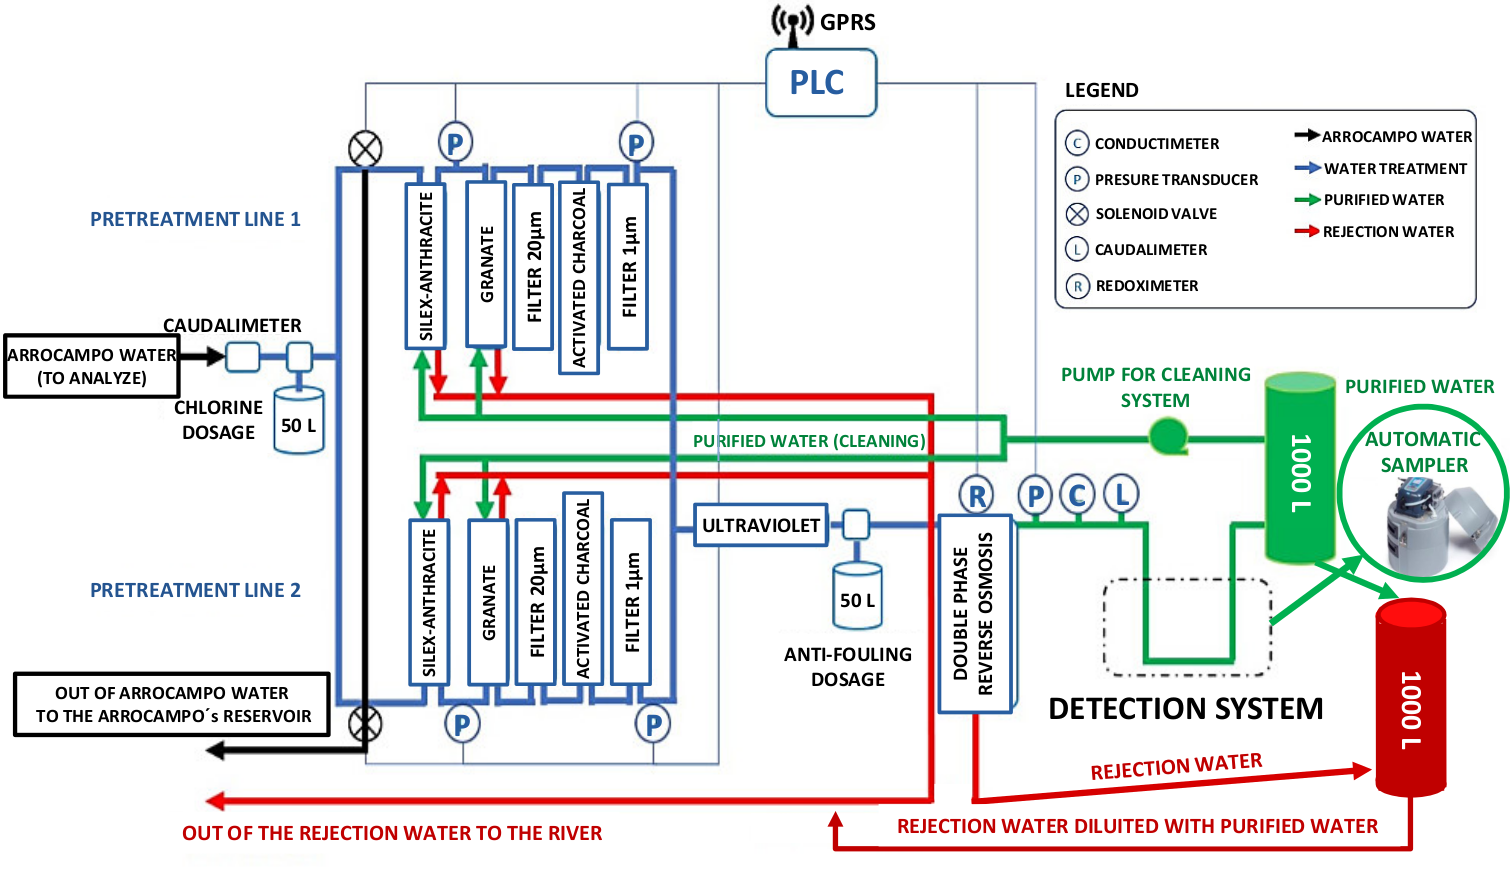
\includegraphics[scale=0.25]{3DesignPrinciples/33UltraPureWaterSystem/SchemeUltraPureWaterSystem.png}
\caption{Scheme of water purification system.\label{fig:WPSScheme}}
\end{figure}

This system is installed in the Arrocampo dam and consists of four different consecutive stages:

\begin{enumerate}
\item{} The raw water from the Tagus River passes through two different filters, the first made of silex-anthracite and the second of garnet, with which a rough filtering is made (the largest particles are eliminated). This system has two parallel lines and implements self-cleaning by injecting ultrapure water in the opposite direction.

\item{} The outlet water sample of the first stage, called fine filtration stage, passes through a $20~\mu\meter$ filter (formed by a synthetic mesh) and activated charcoal filters (one per line) that removes chlorine and iron particles.

\item{} The outlet water of the second stage passes through a super-fine filtering consisting of a $1~\mu\meter$ filter, formed of a dense polypropylene mesh and UV lamps. The first filter removes all the particles up to diameters of $1~\mu\meter$ and the UV lamps remove the organic matter present in the sample.

\item{} Finally, the water is introduced in the last stage, double-phase reverse osmosis, that reduces the conductivity of the water to about $5~\mu$S$/\cm$. It was verified that a conductivity of $10~\mu$S$/\cm$ is achieved with only one module of reverse osmosis, enough for the needed conditions of tritium detector. Therefore, only one module of reverse osmosis is used, reducing the power consumption of the system.

\end{enumerate}

As a result of the purification process, besides the ultrapure water that is introduced into TRITIUM detector, a rejection water, with conductivities greater than the original water containing the particles extracted from the ultrapure water is produced.

The ultrapure water system is able to process up to $0.850~\meter^3/\hour$ with a single line operating or $1.480~\meter^3/\hour$ with both, greatly overestimating the requirements of the tritium detector. 

The software used for remote controlling of the ultrapure water system is Siemens PLC, that gives the information such as the state of the valves, the pressure probes or water production in real time. 

The appendix \ref{App:UltraPureWaterSystem} contains several pictures of different parts of this system, installed in Arrocampo dam.
		%\newpage	
	
	\section[Background Rejection System]{Background Rejection System of the TRITIUM Monitor}\label{sec:IntroductionBackground}
	The aim of the background rejection system is to reduce the radioactive and cosmic background that affects to the TRITIUM monitor. The TRITIUM project follows the ALARA principle for the tritium activity measurement, that is, to measure tritium activity "as low as reasonably achievable". The detection limit of tritium activity is set by the uncertainty in the activity of the background of the natural radioactivity measured by the TRITIUM detector, since tritium activities below this uncertainty cannot be distinguished from the background. Therefore, the background uncertainty must be reduced as much as possible. The total uncertainty is the quadratic sum of all the different uncertainties related to the measurement, i.e., the statistical uncertainty\footnote{Uncertainty due to the statistical nature of the radioactivity process}, $\sigma_{st}$, the systematic uncertainty\footnote{uncertainty due to the manufacturing process of the detectors}, $\sigma_{si}$, etc. Because of the Poissonian nature of the process, the statistical uncertainty is given by the square root of the measured activity, $A_{m}$, which can be reduced by minimizing detected background events.

\begin{equation}
\sigma_{T}^2 = \sigma_{st}^2 +\sigma_{si}^2; \qquad \qquad \sigma_{st;bak} = \sqrt{A_{m;bak}}
\label{eq:SquareSumUncerainty}
\end{equation} 

The background rejection system of the TRITIUM monitor reduces the background activity measured by the TRITIUM detector, minimizing the statistical component of the background uncertainty.

The background of TRITIUM has two different sources. On the one hand, radioactive elements that are present in the crust of the Earth, mainly $\ce{^{40}K}$ and elements from the four different natural radioactive series, shown in Table \ref{tab:NaturalRadioactiveSeries}. On the other hand, the cosmic ray radiation. The primary cosmic radiation, of extra-terrestrial origin, is composed of high-energy particles, mainly protons and $\alpha$ particles, which interact with the Earth's atmosphere and generate a shower mainly composed by muons, electrons, photons and neutrons.

\begin{table}[htbp]
\centering{}%
\begin{tabular}{lcccc}
\toprule 
Mass Num. & Series & Primary & Half life (y) & Final \tabularnewline
\midrule
\midrule 
4n & Thorium & $\ce{^{232}Th}$ & $1.41 \cdot{} 10^{10}$ & $\ce{^{208}Pb}$ \tabularnewline
4n+1 & Neptunium & $\ce{^{237}Np}$ & $2.14 \cdot{} 10^{6}$ & $\ce{^{209}Pb}$ \tabularnewline
4n+2 & Uranium-Radium & $\ce{^{238}U}$ & $4.51 \cdot{} 10^{9}$ & $\ce{^{206}Pb}$ \tabularnewline
4n+3 & Uranium-Actinium & $\ce{^{235}U}$ & $7.18 \cdot{} 10^{8}$ & $\ce{^{204}Pb}$ \tabularnewline
\bottomrule
\end{tabular}
\caption{Classification of natural radioactive series \cite{NaturalRadioactiveSeries1, NaturalRadioactiveSeries2}. The information displayed for each radioactive series is the multiplicity of the mass number, the name of the series, the primary and final element, and the half-life of the primary element.}
\label{tab:NaturalRadioactiveSeries}
\end{table}
Cosmic radiation depends on several parameters like the longitude, latitude, and the solar activity cycle. The spatial distribution of cosmic rays, mainly muons, follows a $cos^2(\theta)$ distribution with the zenith angle. 

Two different techniques are employed for background suppression:

\begin{enumerate}

\item{}  The soft background component, with energy below $200~\MeV/$nucleon, is stopped by a lead castle, described in section \ref{subsec:SetUpPassiveShield},

\item{} The hard background component, with energy greater than $200~\MeV/$nucleon, is much more difficult to stop and the technique employed is the use of a cosmic veto in anti-coincidence with the TRITIUM detector, reported in section \ref{subsec:SetUpActiveShield}. %that is, we will save the measured tritium event just when we don't measure any hard cosmic event in time coincidence.

\end{enumerate} 
	%\newpage
	
		\subsection{Passive Shield (Lead)}\label{subsec:SetUpPassiveShield}
		The soft background component is suppressed by a lead shield inside which the TRITIUM detector is placed. This lead shield is efficient for suppressing radiation that originates from the Earth's natural radioactivity and the soft component of cosmic radiation with energies below $200~\MeV$. This lead shield consists of $158$ low intrinsic radioactivity lead bricks of $25~\mm$ thickness. The bricks are chevron shaped, as shown in Figure \ref{fig:LeadBrick}, specially designed for a perfect fit and easy assembly. As can be seen in Figures \ref{subfig:TwoLayers} and \ref{fig:LeadBricksAndArrangement}, these lead bricks are arranged in two layers with a total thickness of $50~\mm$. 
\begin{figure}[h]
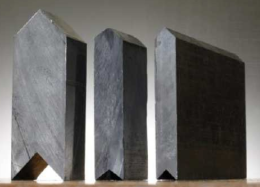
\includegraphics[scale=0.6]{3DesignPrinciples/34BackgroundRejectionSystem/LeadBricks.png}
\centering
\caption{Lead bricks.\label{fig:LeadBrick}}
\end{figure}
\begin{figure}[h]
\centering
    \begin{subfigure}[b]{0.5\textwidth}
    \centering
    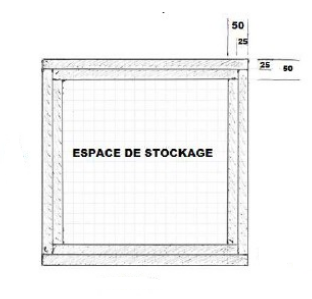
\includegraphics[width=\textwidth]{3DesignPrinciples/34BackgroundRejectionSystem/TwoLayers.png}  
    \caption{\label{subfig:TwoLayers}}
    \end{subfigure}
    \hfill
    \begin{subfigure}[b]{0.4\textwidth}
    \centering
    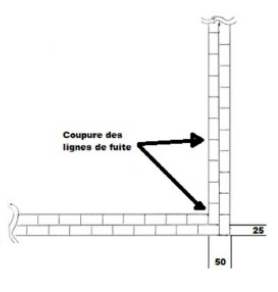
\includegraphics[width=\textwidth]{3DesignPrinciples/34BackgroundRejectionSystem/TwoLayers2.png}  
    \caption{\label{subfig:TwoLayers2}}
    \end{subfigure}
 \caption{Two layers for the lead bricks of the shield. a) General view of the lead castle. b) Detail of the lead brick arrangement.}
 \label{fig:LeadBricksAndArrangement}
\end{figure}
An aluminium structure capable of supporting the total weight of $2.4$ tons of lead bricks, shown in Figure \ref{fig:AluminiumStructure}, was designed by the Mechanical Engineering Department of the CENBG.
\begin{figure}
\centering
    \begin{subfigure}[b]{0.5\textwidth}
    \centering
    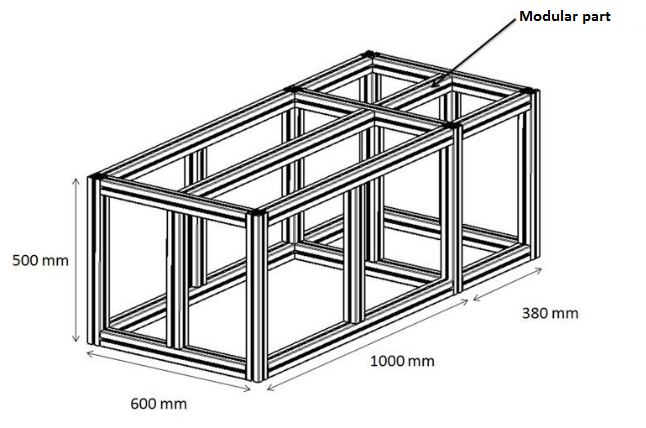
\includegraphics[width=\textwidth]{3DesignPrinciples/34BackgroundRejectionSystem/AluminiumStructureScheme.png}  
    \caption{\label{subfig:AluminiumStructureScheme}}
    \end{subfigure}
    \hfill
    \begin{subfigure}[b]{0.45\textwidth}
    \centering
    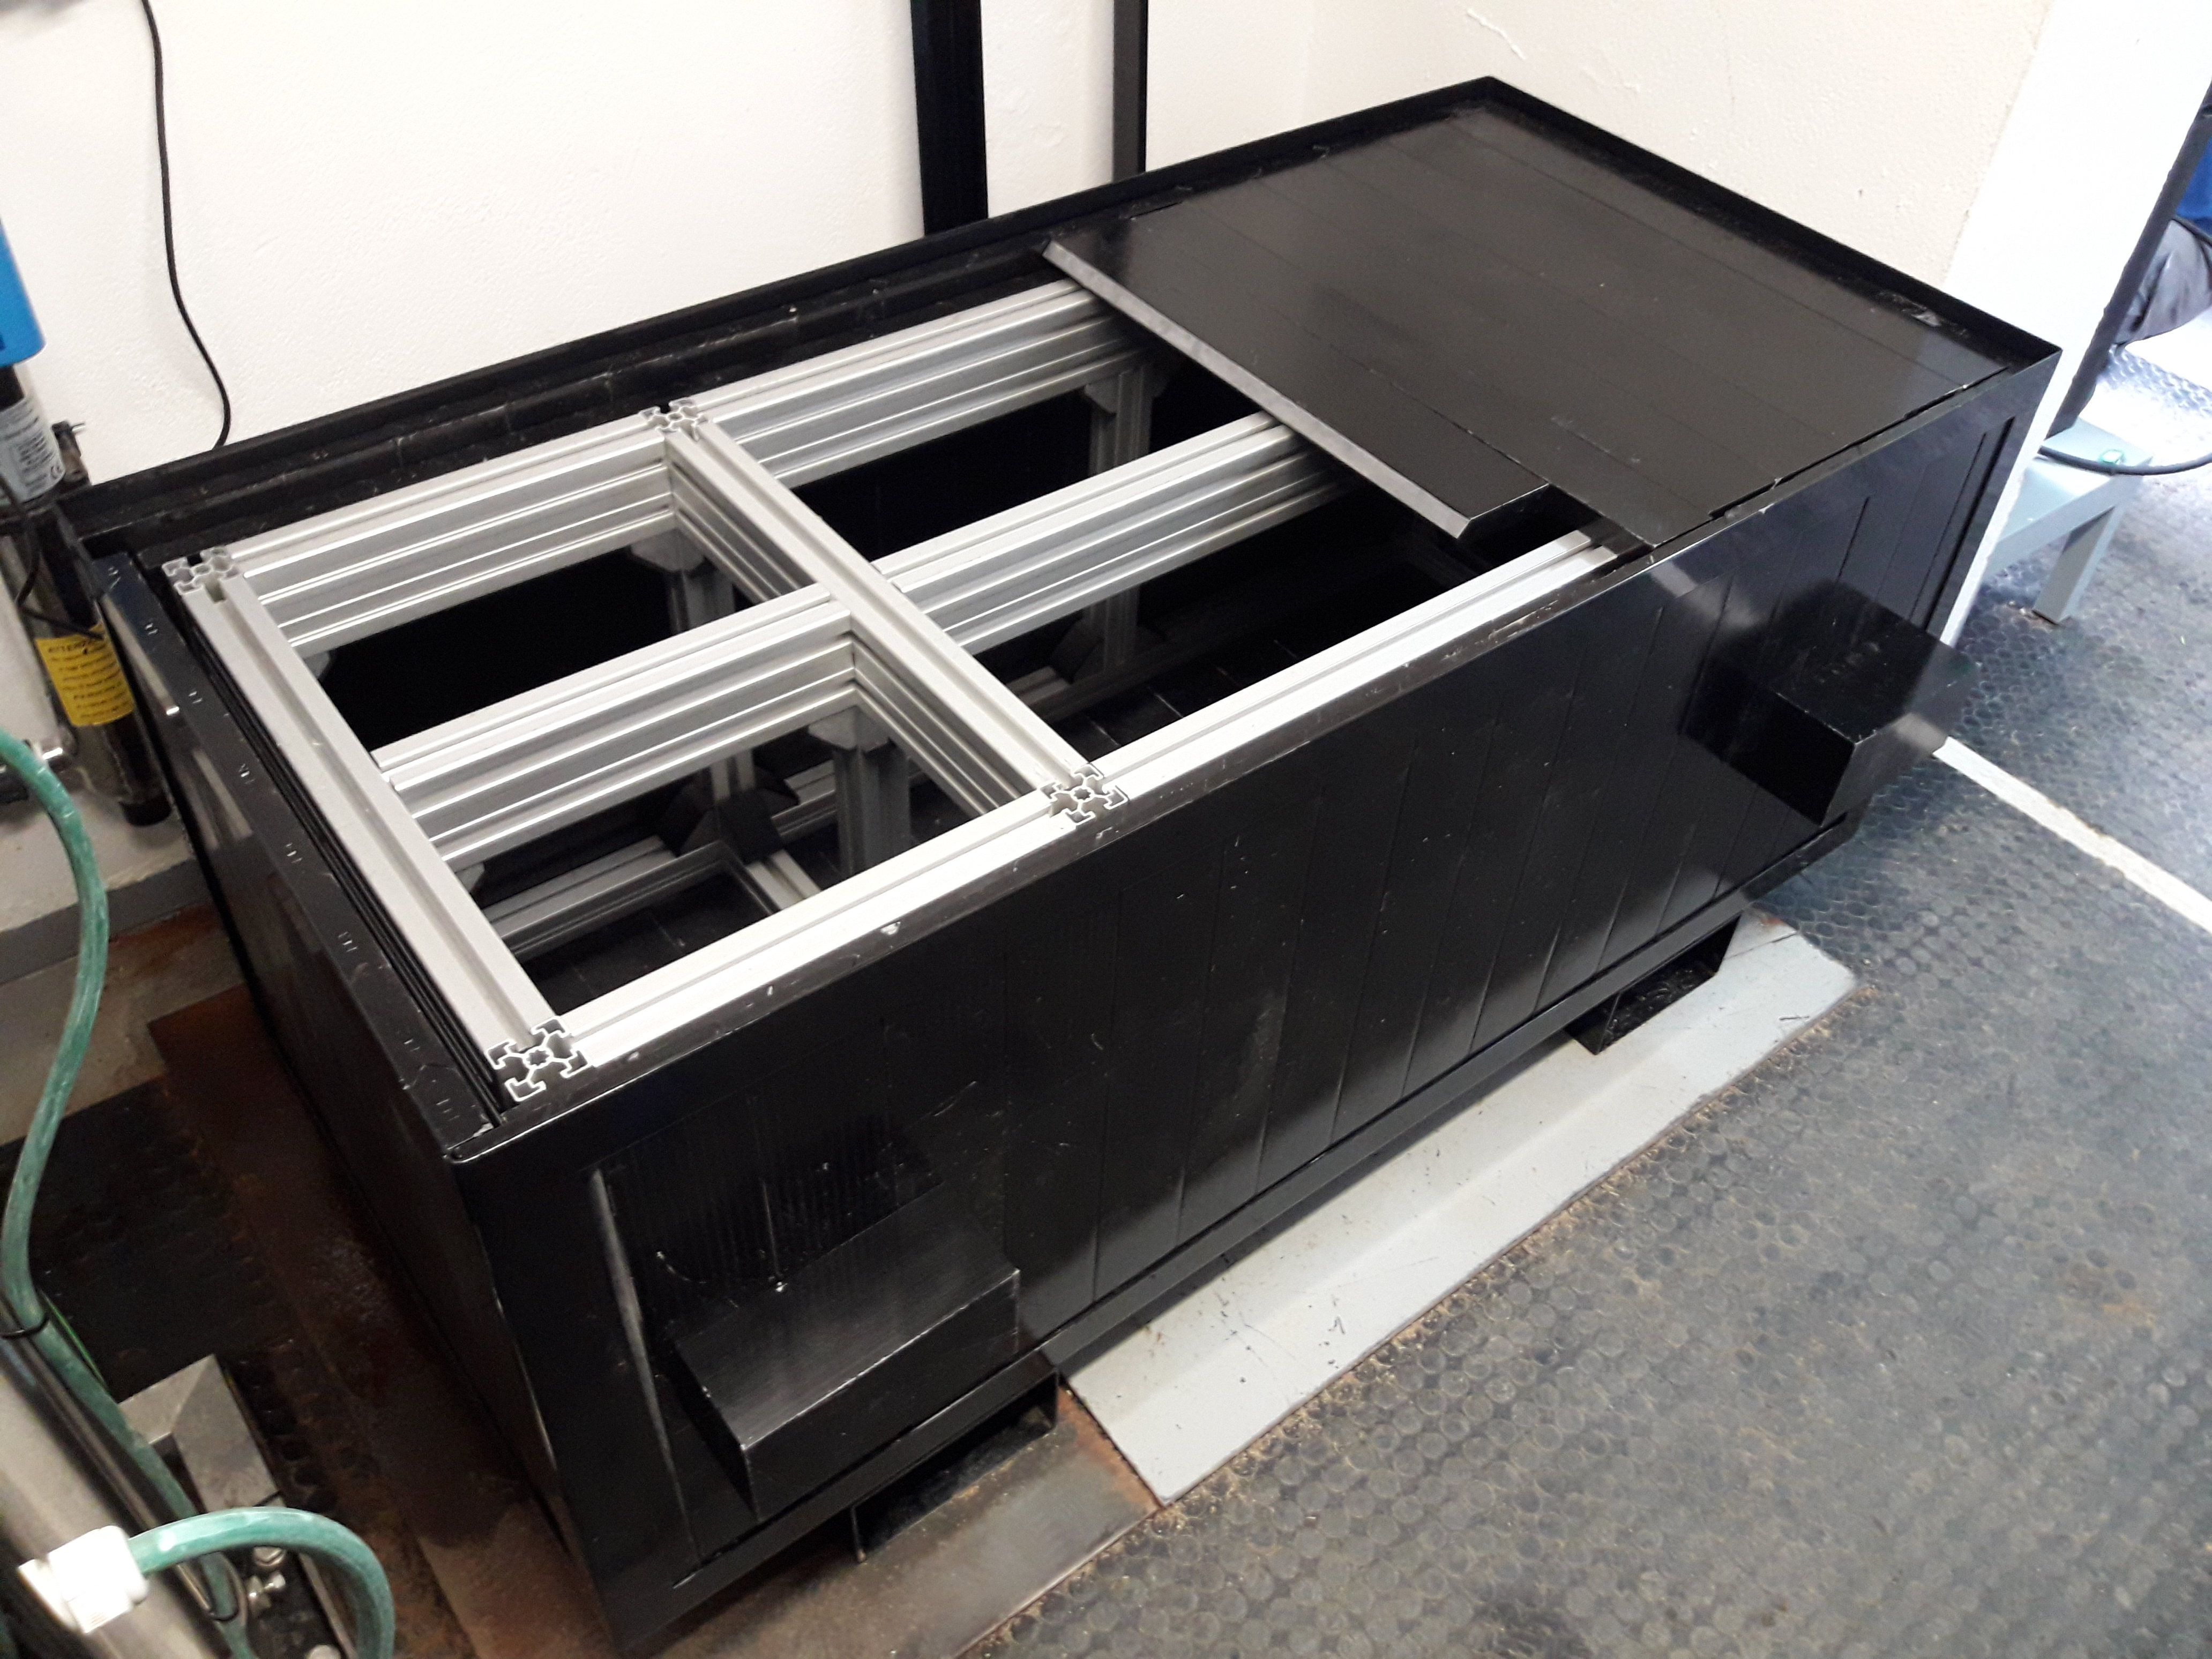
\includegraphics[width=\textwidth]{3DesignPrinciples/34BackgroundRejectionSystem/AluminiumStructure.jpg}  
    \caption{\label{subfig:AluminiumStructure}}
    \end{subfigure}
    \caption{a) Scheme of the aluminium structure of the shield. b) The lead shield partially mounted.}
 \label{fig:AluminiumStructure}
\end{figure}
The internal room of the lead shield is divided into two parts, as indicated in Figure \ref{fig:AluminiumStructure}. The larger one has internal dimensions of $90.5 \times 41 \times 51~\cm^3$ and is used to place the TRITIUM detector. The smaller one, with dimensions of $33 \times 41 \times 51~\cm^3$, contains the DAQ system of the detector. The external dimensions of the lead shield are $148 \times 60 \times 70~\cm^3$ and its total weight is $2.5$ tons.
		%\newpage
		
		\subsection{Active Shield (Cosmic Veto)}\label{subsec:SetUpActiveShield}
		As hard radiation cannot be stopped by a moderate lead thickness so cosmic vetos are employed, which consists of at least two complementary detectors in coincidence that reject events simoultaneously detected in both. 

As shown in Figure \ref{fig:VetoAndPrototype}, the two complementary detectors are placed one above and the other below the TIRTIUM detector. The distance between both detectors, $34.2~\cm$ for our latest prototype developed, is set by the TRITIUM prototype to be placed between both.

\begin{figure}[h]
\centering
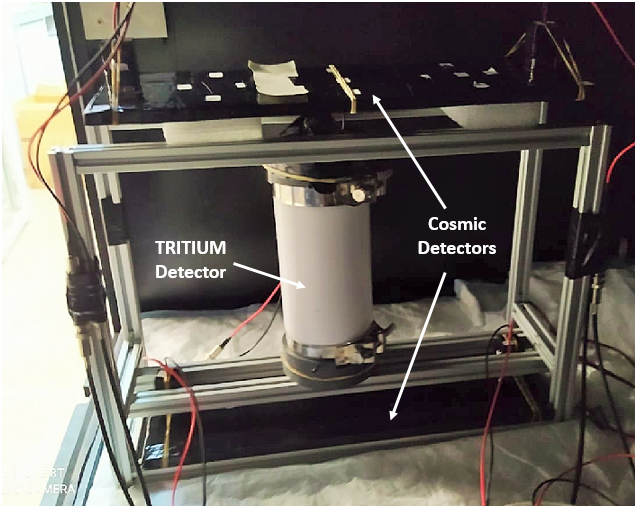
\includegraphics[scale=0.45]{3DesignPrinciples/34BackgroundRejectionSystem/Vetos_y_prototipo.png}
\caption{Cosmic veto and Tritium-IFIC 2 prototype in an aluminum mechanical structure developed by IFIC's mechanical engineering department.\label{fig:VetoAndPrototype}}
\end{figure}

A hard cosmic event simultaneous through both cosmic detectors is schematically shown in figure \ref{subfig:RealHardCosmicEvent}. Each cosmic detector has two photosensors so the electronic configuration given in Figure \ref{subfig:ElectronicConfiguraiton4PMT} is used in each active veto to make time coincidences. The TRITIUM detector is read out in anti-coincidence with the cosmic veto to rejected the hard cosmic events from the tritium measurement. Random coincidence from two different hard cosmic events, one in each detector, shown in Figure \ref{subfig:FakeHardCosmicEvent} are negligible. The expected hard cosmic rate at sea level for muons, main contributor, is $70~\meter^{-2}\second^{-1}\steradian^{-1}$ \cite{PDG, HardCosmicMuonRate}, that is $7\times 10^{-3}~\cm^{-2}\second^{-1}\steradian^{-1}$, shown in the cosmic rate plot of Figure \ref{fig:HardCoscmicRate}. As time coincidences are triggered by logical gates of about $10~\nano\second$, the probability of recording two different hard cosmic events in temporal coincidence is less than $10^{-9}$ which is not worth considering.

\begin{figure}
\centering
    \begin{subfigure}[b]{0.45\textwidth}
    \centering
    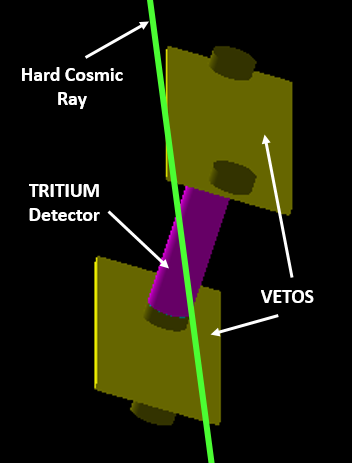
\includegraphics[width=\textwidth]{3DesignPrinciples/34BackgroundRejectionSystem/Real_Event.png}  
    \caption{Real hard cosmic event.\label{subfig:RealHardCosmicEvent}}
    \end{subfigure}
    \hfill
    \begin{subfigure}[b]{0.45\textwidth}
    \centering
    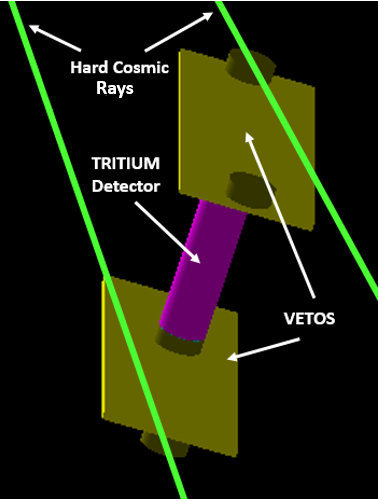
\includegraphics[width=\textwidth]{3DesignPrinciples/34BackgroundRejectionSystem/Fake_Event.png}  
    \caption{Fake hard cosmic event.\label{subfig:FakeHardCosmicEvent}}
    \end{subfigure}
   \caption{Hard cosmic events detected with the cosmic veto of TRITIUM: a) Affecting to the tritium measurement, b) Does not affecting to the tritium measurement.}
 \label{fig:HardCosmicEventsSimulation}
\end{figure}

\begin{figure}[h]
\centering
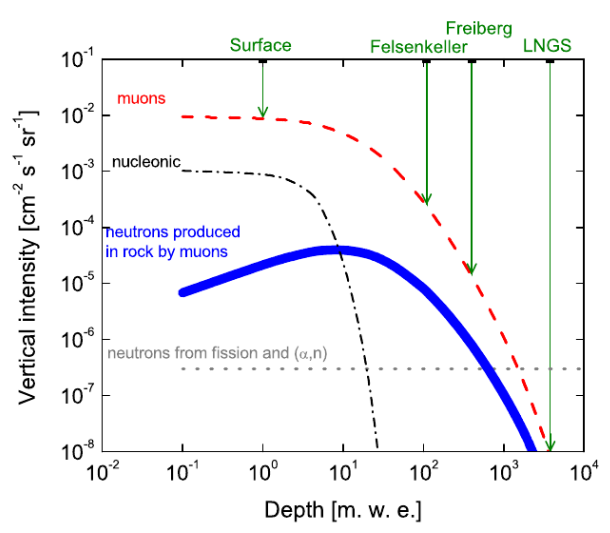
\includegraphics[scale=0.6]{3DesignPrinciples/34BackgroundRejectionSystem/HardCosmicRate.png}
\caption{Hard cosmic muon rate \cite{HardCosmicMuonRatePlot}.\label{fig:HardCoscmicRate}}
\end{figure}

The vetos are made of a plastic scintillator block from Epic-Crystal \cite{ScintillatorVeto}. Its properties are given in Table \ref{tab:ParametersScintillatorVeto} and its energy emission spectrum is displayed in Figure \ref{fig:EmissionEnergySpectrumVeto}.

\begin{table}[]
%%\centering
\begin{center}
\begin{tabular}{|c|c|c|}
%\hline
%Material & Refractive index \\
\hline \hline 
Base material & Polystyrene \\ \hline
Growth method & Polymeric \\ \hline
Density ($\gram/\cm^3$)& 1.05 \\ \hline
Refractive index & 1.58 \\ \hline
Soften temperature ($\degree$) & 75-80 \\ \hline
Light output (Anthracene) & 50-60\% \\ \hline
H/C raito & 1.1 \\ \hline
Emission peak (nm) & 415 (Blue) \\ \hline
Decay Time, (ns) & 2.4 \\ \hline
Hygroscopic & No \\ \hline
\end{tabular}
\caption{Properties of plastic scintillators from Epic-Crystals. \cite{ScintillatorVeto}}
\label{tab:ParametersScintillatorVeto}
\end{center}
\end{table}

\begin{figure}[]
\centering
\includegraphics[scale=0.35]{3DesignPrinciples/34BackgroundRejectionSystem/EmissionEnergySpectrumVetos.png}
\caption{Emission energy spectrum of the plastic scintillation used for the cosmic vetos.\label{fig:EmissionEnergySpectrumVeto}~\cite{ScintillatorVeto}}
\end{figure}

The energy spectrum has a peak very close to that of the scintillating fibers used, so the same photosensors are used to read out them. The dimensions of the scintillator block are $45 \cdot{} 17 \dot{} 1~\cm^3$ and they are wrapped by three different layers, teflon, aluminum and black tape, exhibited in Figure \ref{fig:LayersVeto}. These layers prevent external photons from reaching the scintillator plastic and avoid photons generated by the scintillator plastic from escaping before reaching the photosensor. Two $2.5\times 2.5 ~\cm^2$ windows are made on the wrapping to allow reading by the photosensors.


\begin{figure}
\centering
    \begin{subfigure}[b]{0.23\textwidth}
    \centering
    \includegraphics[width=\textwidth]{3DesignPrinciples/34BackgroundRejectionSystem/NoCoating.jpeg}  
    \caption{Scintillator without coating.\label{subfig:PlasticScintillatorNoCoating}}
    \end{subfigure}
    \hfill
    \begin{subfigure}[b]{0.23\textwidth}
    \centering
    \includegraphics[width=\textwidth]{3DesignPrinciples/34BackgroundRejectionSystem/TeflonCoating.jpeg}  
    \caption{Teflon coating.\label{subfig:PlasticScintillatorTeflon}}
    \end{subfigure}
    \hfill
    \begin{subfigure}[b]{0.23\textwidth}
    \centering
    \includegraphics[width=\textwidth]{3DesignPrinciples/34BackgroundRejectionSystem/AluminiumCoating.jpeg}  
    \caption{Aluminium coating.\label{subfig:PlasticScintillatorAluminium}}
    \end{subfigure}
    \hfill
    \begin{subfigure}[b]{0.23\textwidth}
    \centering
    \includegraphics[width=\textwidth]{3DesignPrinciples/34BackgroundRejectionSystem/BlackTapeCoating.jpeg}  
    \caption{Black tape coating.\label{subfig:PlasticScintillatorBlackTape}}
    \end{subfigure}
 \caption{Different layers used to cover of the cosmic veto.}
 \label{fig:LayersVeto}
\end{figure}

As previously mentioned, the expected hard cosmic rate at sea level is $7 \times 10^{-3}~\cm^{-2}\second^{-1}\steradian^{-1}$. Taking into account that the solid angle of our detectors is $\omega=0.5434$, calculated by integrating the solid angle of one scintillator on the other, and the area of the veto is $765~\cm^2$, the expected hard cosmic rate on our cosmic vetos should be $2,909~$event$/\second$. This is an important result which is used in section \ref{sec:TritiumActiveVeto} to determine the efficiency of the cosmic veto.
		\newpage
					
\chapter[TRITIUM Detector R\&D]{Research \& Development on Detector Design and Components}\label{chap:ResearchandDevelopment}
	%\section{Introduction}\label{sec:IntroCharacterisation}
	This chapter describes the characterization of the different parts of the TRITIUM monitor, including scintillating fibers, SiPMs, the water purification system and the background rejection system. This characterization is crucial to understand the behaviour of the different parts and the results of the monitor. Furthermore, several developments were made  to improve fundamental parameters of the TRITIUM monitor components to enhance their tritium sensitivity. All these studies were carried out inside a special light-tight box, called black box, to ensure that the detected photons come from the sources used, either LEDs or scintillators. In addition, as the energy response of plastic scintillators has a rather large uncertainty, most of the energy spectra are shown in ADC\footnote{ADC units are the internal units, called channels, in which an analog signal is digitized after an Analog-to-Digital Converter. The ADC units are proportional to the energy and the number of available channels depends on the bits used in its digitization.} channels, which are linearly proportional to energy.
	%\newpage
	
	\section[R\&D for the Plastic Scintillating Fibers]{R\&D for the Plastic Scintillating Fibers}\label{sec:CharacterizationScintillatingFibers}
	%\input{./Sections/3ResearchAndDevelopment/32CharacterizationFibers}
	%\newpage
	
		%\subsection{Introduction}\label{subsec:IntroFibersResults}
		This section reports experimental measurements of the scintillating fiber parameters that most affect the tritium detection, such as collection effficiency and conditioning uncertainty. Errors are included in all graphs displayed in this section but they are to small to be visible. Thousands of scintillating fibers are used in TRITIUM detector which were prepared and conditioned prior to characterization studies or tritium detection. Therefore, various mechanical and electronical devices were developed to automatically prepare many fibers at the same time.
		%\newpageand
		
		\subsection[Scintillating Fibers Conditioning Protocol.]{Scintillating Fiber Conditioning Protocol.}\label{subsec:ConditioningProcess}
		First thing we had to do in TRITIUM experiment was to choose the optimal fiber length at which the signal from the tritium events is optimized. To make this decision we have to take into account that, on the one hand, long fibers are interesting because the efficiency of our detector is proporcional to the active area, which is proporcional to the fiber length but, on the other hand, in long fibers, scintillation photons will need to be reflected in the fiber walls more times to be driven to its ends, where it will be detected by photosensors and this is a problem because we lose photons in each reflection, deteriorating the detector signal.

Several simulations were performed using Geant4 \cite{Geant4WebPage}, a particle and nuclear physics simulation package based on C++, to quantify, between other things, the importance of this effect and to allow us to choose the optimal fiber length. The results of this simulations will be shown in section \ref{sec:ResultsSimulations}, where they will be discussed. In these simulations it has been seen that it is preferable to work with short fiber (Figure \ref{}). The fiber length, which has been chosen for the tritium prototypes developed in Valencia, is $20~\cm$ and the fiber length used in each study will be named in the appropriate section, but it will be close to this value.

Saint-Gobain's commercial fibers are 1 meter long, so first thing we had to do was cut the scintillation fibers before using it. It is very important to introduce strict requirements on the cutting quality of the fiber ends since it will greatly affect the transmission of photons and, thus, the efficiency of TRITIUM monitor. This cut must be perpendicular to the fiber and very low uncertainty in the length of the fiber, both requeriments are mandatory to achieve a good coupling with the surface of the photosensor. It is also important that its final state must be as clean as possible, that is, without cracks or deformations because it will contribute to internal reflections, losing photons and, thus, reducing the tritium signal.

Cutting the end faces of polymer fibers is one of current challenges. There are many different techniques such as milling, laser cutting, focused-ion-beam, blade cutting, etc. Due to its simplicity, we have focused on blade cleaving. %I had these references in the "Smooth end face termination of microstructured, graded-index, and step-index polymer optical fibers" paper

Many commercial devices based on blade cleaving, such as the one provided by thorlabs with a diamond tipped blade \cite{DiamondThorlabs} or others similar to the guillotine designed for industrial fiber optics \cite{GuillotineIFO}, were tested in a extensive study done but with unsuccessful results \cite{TFGAlberto}. As can be seen in Figures \ref{fig:BadCutsOfFibers}, it presents deformations, cracks or imperfections so the technics considered in this study don't overcome the requirements imposed.

\begin{figure}[htbp]
 \centering
  \subfloat[Fiber end deformation.]{
   \label{subfig:FiberEndDeformation}
    \includegraphics[width=0.5\textwidth]{4ResearchAndDevelopments/41Fibers/DeformationFiberEnds.png}}
    %\newline
  \subfloat[Fiber end cracks.]{
   \label{subfig:FiberEndCracks}
    \includegraphics[width=0.45\textwidth]{4ResearchAndDevelopments/41Fibers/CracksEndFibers.png}}
 \caption{Unsuccessful results of using commercial techniques to cut fibers.}
 \label{fig:BadCutsOfFibers}
\end{figure}

The microscope model PB 4161 from EUROMEX company or the Digital Microscope from Jiusion company, shown in Figures \ref{fig:Microscopes}, were used to check the results in the fiber ends.

\begin{figure}[htbp]
 \centering
  \subfloat[EUROMEX microscope]{
   \label{subfig:EUROMEXMicroscope}
    \includegraphics[width=0.25\textwidth]{4ResearchAndDevelopments/41Fibers/EuromexMicroscope.png}}
    %\newline
  \subfloat[Jiusion microscope]{
   \label{subfig:JiusionMicroscope}
    \includegraphics[width=0.45\textwidth]{4ResearchAndDevelopments/41Fibers/JiusionMicroscope.png}}
 \caption{Microscopes used to check the results.}
 \label{fig:Microscopes}
\end{figure}

Because commercial devices don't work for our scintillating fibers, we had to design, build and test our own cutting device, which is shown in Figure \ref{fig:CuttingTRITIUMDevice}.

\begin{figure}[htbp]
 \centering
  \subfloat[TRITIUM Cutting device]{
   \label{subfig:CuttingDevice1}
    \includegraphics[width=0.4\textwidth]{4ResearchAndDevelopments/41Fibers/CuttingDevice1.png}}
    %\newline
  \subfloat[TRITIUM Cutting device]{
   \label{subfig:CuttingDevice2}
    \includegraphics[width=0.55\textwidth]{4ResearchAndDevelopments/41Fibers/CuttingDevice2.png}}
    \newline
    \subfloat[Additional piece of TRITIUM cutting device]{
   \label{subfig:AdditionalPieceCuttingDevice}
    \includegraphics[width=0.6\textwidth]{4ResearchAndDevelopments/41Fibers/AdditionalPieceCuttingDevice.png}}
 \caption{Cutting device developed in the TRITIUM experiment and additional part to make precise measurements of fiber length.}
 \label{fig:CuttingTRITIUMDevice}
\end{figure}

It consists of fourteen rails where the fibers will be fixed and a thin blade, fixed on a mobile piece, perpendicular to the fibers, with which we can be sure of achieving a perpendicular cut, which is one of the requirements imposed.

The blade used is the typical commercial razor blade, whose thickness is $0.1~\mm$, which is the thickness with which we obtain the best results and it was positioned with a slight inclination, $5\degree$, with respect to the horizontal axis since it has been seen in several studies that this helps to obtain a less aggressive and cleaner cut  \cite{AngleBlade}, \cite{TemperatureBlade}.

Therefore, as can be seen in Figure \ref{subfig:CutFiberEnd}, with this device we obtain fiber ends without breaks or deformation overcoming another imposed requirement.

Another important parameter that can affect the cutting quality of the fiber ends is the temperature of both, either the fiber or the blade. It has been tested in a study in which both were subjected to different temperatures from room temperature (25 degrees) to 110 degrees \cite{TFGAlberto}. No significant conclusions were obtained in the temperature study, so we work at room temperature to facilitate the cutting technic.

To obtain a low enough length uncertainty, which is the last requirement we must overcome, we designed and built an additional piece, shown in Figure \ref{subfig:AdditionalPieceCuttingDevice}, which is used to measure the fiber. With this piece we achieve an uncertainty in the measurement of less than 1 millimeter.

With the designed cutting fiber device we have exceeded all requirements imposed, obtaining a cut fiber end whose quality is high enough to ensure that it will affect the transmission of light as little as possible.

In Figure \ref{subfig:CutFiberEnd}, which shows the fiber end after cutting process with TRITIUM cutting device, you can see a slightly darkened part at the bottom of the fiber, which is an inevitable effect of the cutting process. To repair this imperfection, a polishing process developed by thorlabs is included \cite{DiamondThorlabs}. 

This polishing process consists of using five different polishing papers, with a decreasing grain size, whose diameters are $30~\mu\meter$, $20~\mu\meter$, $12~\mu\meter$, $5~\mu\meter$ and $0.3~\mu\meter$ respectively, in which we describe movements in the shape of 8 for two minutes (approximately 120 movements). 

The result obtained with this polishing process is shown in Figure \ref{subfig:PolishFiberEnd}. In Figure \ref{fig:ResultofPolishingProcess}, the quality of both fiber ends, before and after polishing process, can be compared. There, we can see that the darkened part has completely disappeared. 

\begin{figure}[htbp]
 \centering
  \subfloat[Fiber end after cutting with Tritium device.]{
   \label{subfig:CutFiberEnd}
    \includegraphics[width=0.5\textwidth]{4ResearchAndDevelopments/41Fibers/CutEndFiberGood.png}}
    %\newline
  \subfloat[Fiber end after cutting and polishing.]{
   \label{subfig:PolishFiberEnd}
    \includegraphics[width=0.45\textwidth]{4ResearchAndDevelopments/41Fibers/CutAndPolishedFiberEnd.png}}
 \caption{Result of the polishing process. a) Fiber end after cutting with TRITIUM devices b) Fiber end after cutting with TRITIUM devices and polishing with Thorlabs technic.}
 \label{fig:ResultofPolishingProcess}
\end{figure}

The end of the cut fiber is completely clear after cutting and polishing, without any damage or imperfection, so both tasks, cutting and polishing, will make up the conditioning process developed for each fiber before any study or its introduction into the TRITIUM detector.
		%\newpage
				
		\subsection[Automatic Polishing Machine]{Automatic Polishing Machine for Scintillating Fibers}\label{subsec:PolishingMachine}
		As mentioned above, tens of thousands of fibers had to be prepared and conditioned for the TRITIUM monitor\footnote{Tritium prototype will be a module of TRITIUM monitor, based on dozens of modules.}, section \ref{sec:TritiumMonitor}. Although this number of fibers was not a problem for cleaving, which is very fast process, the polishing process is quite time consuming. It takes more than ten minutes to polish each fiber, that would result in an unaffordable amount of time to prepare the needed quantity of fibers. Therefore, an automatic polishing machine for scintillating fibers was designed, built and tested. This polishing machine is able to polish up to one hundred scintillating fibers at the same time and automatically. Furthermore, it is easily scalable to larger number of fibers.

\begin{figure}[h]
\centering
\includegraphics[scale=0.75]{4ResearchAndDevelopments/41Fibers/GeneralViewPolishingMchine.png}
\caption{Polishing machine developed in TRITIUM experiment.\label{fig:GeneralViewPolishingMachine}}
\end{figure}
This automatic polishing machine, displayed in Figure \ref{fig:GeneralViewPolishingMachine}, consists of two parts: 1) A polishing table, where the fibers are polished 2) The electronics, based on Arduino technology, that operates the movement of the polishing table:

\begin{enumerate}
\item{} The polishing table, shown in Figure \ref{subfig:PolishingTable}, is divided in two parts: the static part, where the fibers are fixed, and the movable part, where the polishing papers are fixed. It was decided to set the polishing papers on the movable part because they are lighter and less fragile than fibers.

The static part consists of a piece, shown in Figure \ref{subfig:PolishingTable}, built with a 3D printer and locked to the system by four vertical screws. There are two nuts on each screw used to set the relative height and the inclination of fibers to the polishing papers. This piece contains one hundred holes in which the fibers are placed. 

As the fibers are too light ($0.16~\gram$) to make the necessary pressure on the polishing paper, a plastic belt and a piece of metal with a weight of around $1.5~\gram$, shown in Figure \ref{subfig:FiberMetailcPiece}, were employed to increase their contact pressure (similar to the connectors used in the Thorlabs polishing process). 

The movable part consists of a flat PMMA plate of $18 \times 18~\cm^2$ to which the polishing paper is attached. This part is locked to two horizontal screws, perpendicular to each other that are used to set its position in the XY plane (horizontal plane), as shown in Figure \ref{subfig:HorizontalAxis}.

The polishing system contains several switches,  mounted on a piece made with the help of a 3D printer, shown in Figures \ref{subfig:PolishingTable}, \ref{subfig:HorizontalAxis} and \ref{subfig:3DSwitchPiece}, which are used to find the origin of coordinates when the system is reinitiated and to stop the movable part when the end of the path is reached. 

\begin{figure}
\centering
    \begin{subfigure}[b]{0.55\textwidth}
    \centering
    \includegraphics[width=\textwidth]{4ResearchAndDevelopments/41Fibers/PolishingTable.png}  
    \caption{Polishing table.\label{subfig:PolishingTable}}
    \end{subfigure}
    \hfill
    \begin{subfigure}[b]{0.3\textwidth}
    \centering
    \includegraphics[width=\textwidth]{4ResearchAndDevelopments/41Fibers/PieceOfFiber.png}  
    \caption{Fiber with metal piece.\label{subfig:FiberMetailcPiece}}
    \end{subfigure}
    \hfill
    \begin{subfigure}[b]{0.55\textwidth}
    \centering
    \includegraphics[width=\textwidth]{4ResearchAndDevelopments/41Fibers/HorizontalAxis2.png}  
    \caption{Horizontal screws and PMMA plate.\label{subfig:HorizontalAxis}}
    \end{subfigure}
    \hfill
    \begin{subfigure}[b]{0.4\textwidth}
    \centering
    \includegraphics[width=\textwidth]{4ResearchAndDevelopments/41Fibers/Switch.png}  
    \caption{Piece to hold switches.\label{subfig:3DSwitchPiece}}
    \end{subfigure}
 \caption{Polishing table of the polishing machine.}
 \label{fig:PolishingTable}
\end{figure}

\item{} The electronics which controls the automatic movement of the polishing paper, shown in Figure \ref{fig:ElectronicSystemPolishingMachine}, is based on Arduino technology.

This electronics consists of two stepper motors, model NEMA ST4209S1404-A \cite{StepperMotors}, which move the horizontal screws on which the polishing paper is attached. These motors are controlled by an Arduino UNO \cite{ArduinoUNO} that uses a CNC shield \cite{CNCShield} in which two different drivers are connected to control the stepper motors, one driver for each stepper motor.

Drivers are controllers that allow to manage stepper motors in a simple way. It is very important to choose the correct controller for the system because the controller limits the supply power to the motors, avoiding burning of the motors in the worst case. Instead of using the Pololu A4988 drivers \cite{A4988Driver}, which is one of the most widely used drivers, the first choice was the DRV8825 driver \cite{DRV8825Driver}. DRV8825 allows to power the motor with higher voltage and intensities ($45~\volt$ and $2.5~\ampere$) than A4988 ($35~\volt$ and $2~\ampere$). Also, the DRV8825 controller includes a new microstepping mode ($1/32$) compared to the A4988 ($1/16$) with which we get more accurate and smooth movements. Finally the drivers were replaced by the TMC2208 \cite{TMC2208Driver}, much less noisy since it includes the \textit{StealthChop} function with which the noise is practically eliminated. Furthermore, this controller is much more accurate owing to its a microstepping mode of $1/256$. The voltage and current used to power the motors are $35~\volt$ and $2~\ampere$ which are sufficient for the whole system since the current of the motors is limited to $1.33~\ampere$. The excess current will be transformed into heat that has to be dissipated from the system. Overheating of the drivers may cause loss of steps, producing wrong movements or even destroying the driver. Therefore, a cooling system is needed to ensure the correct operation of the polishing system. The cooling system, shown in Figure \ref{fig:ElectronicSystemPolishingMachine}, consists of a copper piece\footnote{The copper is one of the best thermal conductor at STP} in contact with both controllers and a fan, used to prevent heat accumulation inside the electronics box. The cooling power can be inproved by using a PELTIER cell.

\begin{figure}[h]
\centering
\includegraphics[scale=0.75]{4ResearchAndDevelopments/41Fibers/ElectronicPolishingMachine.png}
\caption{Electronic system of Polishing machine.\label{fig:ElectronicSystemPolishingMachine}}
\end{figure}

\end{enumerate}

This polishing machine is controlled by a Raspberry Pi computer board using the Universal G-code Sender software (a grafical interface based on the GRBL package). There are several useful pre-programmed functions such as "HOME" with which the system, using the switches, finds its origin of coordinate every time the system is turned on. The software also has the possibility of loading a file containing the G-code to be executed. In the TRITIUM project, the 120 movements required for each polishing paper are loaded in this way. This machine was tested with twenty fibers of $15~\cm$ length arranged in a bundle. The fibers were fixed to the structure shown in Figure \ref{fig:BunchWith2PMTsCoincidence} and two PMTs located at the bundle ends, read in coincidence as described in section \ref{subsubsec:PMTsElectronicalSystem}, Figure \ref{subfig:ElectronicConfiguraiton2PMT}, monitored the light transmision of the fibers.

\begin{figure}[]
\centering
\includegraphics[scale=0.6]{4ResearchAndDevelopments/41Fibers/FiberBunch2PMTsCoincidence.png}
\caption{Setup used to test the effect of the polishing machine.\label{fig:BunchWith2PMTsCoincidence}}
\end{figure}

The light transmission was measured before and after polishing. These measurements were carried out using two radioactive sources, a $\ce{^{60}Co}$ gamma source of $715~\becquerel$ activity, and a $\ce{^{90}Sr}$ beta source of $17.8~\kilo\becquerel$ activity. The energy spectra recorded for both radioactive sources are exhibited in Figure \ref{fig:ResultsOfPolishingMachine}. The sources were placed in the middle of the fiber bundle, at $7.5~\cm$ from each PMT.

\begin{figure}
\centering
    \begin{subfigure}[b]{1\textwidth}
    \centering
    \includegraphics[width=\textwidth]{4ResearchAndDevelopments/41Fibers/Co_60_PolishingMachine_ZOOM.pdf}  
    \caption{Energy spectrum recorded for the Co-60 source.\label{subfig:EnergySpectrumCo60PolishingTest}}
    \end{subfigure}
    \hfill
    \begin{subfigure}[b]{1\textwidth}
    \centering
    \includegraphics[width=\textwidth]{4ResearchAndDevelopments/41Fibers/Sr_90_PolishingMchine_ZOOM.pdf}  
    \caption{Energy spectrum recorded for the Sr-90 source.\label{subfig:EnergySpectrumSr90PolishingTest}}
    \end{subfigure}
 \caption{Energy spectra recorded with polished and unpolished fibers.}
 \label{fig:ResultsOfPolishingMachine}
\end{figure}

As it can be seen in Figure \ref{fig:ResultsOfPolishingMachine}, both energy spectra are shifted to the right after polishing, which means that the detected events have more energy (more photons per event reach the PMTs). This energy increase was more than 40\% ($(42 \pm 4.6)\%$ for gamma source and $(49 \pm 8.4)\%$ for beta source) with respect the unpolished fibers. In summary, with the polishing machine, the photon collection efficiency of the fibers was improved  (mainly due to the improvement of the interface between fibers and PMTs). It is very important to achieve a high detection efficiency as the expected number of photons per tritium event is quite low.
		%\newpageand
		
		\subsection{Characterization of Scintillating Fibers}\label{subsec:CharacterizationFibers}
		This section describes the characterization of uncladded BCF-12 fibers, called no-clad fibers, from Saint-Gobain, which are the fibers selected for the TRITIUM experiment. These fibers are compared to single clad and multiclad BCF-12 fibers to quantify the influence of the clad in the relevant parameters of the scintillating fibers.

Although commercial clads are too thick for the TRITIUM experiment, the necessary low thickness clad could be developed. For example, clads with a thickness of the order of tens of nanometers can be achieved by electrodeposition techniques.

The difference between these three types of fibers is that uncladded fibers only consist of a polystyrene core with a refractive index of $1.60$ whereas, single clad fibers, have an acrylic clad (PMMA) of $30~\mu\meter$ thickness and a refractive index of $1.49$ and, multiclad fibers, have a second fluor-acrylic clad of $10~\mu\meter$ thickness  and a refractive index of 1.42.

%The first measurement that was made is the measurement of the diameter of the fiber. It is important because scintillating molecules are only present in the polystyrene core and we need to know whether the entire polystyrene core is the same size or not. Three different samples of each type of fiber were measured and the results are presented in Table \ ref {}.

%TABLAAA DIAMETROOOS

%Therefore, we can see that all fibers have the same external size, which means that the diameter of the polystyrene core is smaller for single clad fibers ($0.97~\mm$) and even smaller for multiclad fibers ($0.96~\mm$). It is an important result since...

This characterization was carried out at the level of a single scintillating fiber. The parameters measured for each fiber type were the fiber collection efficiency and the uncertainty of the fiber response due to the conditioning process. The reference magnitude employed for the characterization is the rate of photons that reach the active area of the photosensor. To measure this magnitude, a calibrated R8520-06SEL PMT was used, whose quantum efficiency at the working wavelength, $29.76\%$, was measured by Hamamatsu. The PCB described in section \ref{subsubsec:PMTsElectronicalSystem} was used for working without the PMT internal gain and the PMT output current was measured by a Keithley 6487 Picoammeter/Voltage Source. The photons rate was obtained from the current measurement using the equation \ref{eq:NumPhotonsFromIntensityPMT} with $QE=0.2976$ and $CE=1$. A simplified scheme of the used set up is shown in Figure \ref{fig:SetUpFiberCharacterization}.

\begin{figure}[h]
\centering
\includegraphics[scale=0.6]{4ResearchAndDevelopments/41Fibers/SetUp_Fiber_Characterization.png}
\caption{Set up used for fiber characterization.\label{fig:SetUpFiberCharacterization}}
\end{figure}

This setup consists of an optical structure in which a LED and a PMT are fixed to a user set distance between them. A LED435-03 from Roithner LaserTechnik Gmbh \cite{LEDRLT}, simulated the light emission by the fibers. The emission spectrum of the LED, given in Figure \ref{fig:LEDSpectrumTritium}, was experimentaly measured by a spectrometer and fitted to a Gaussian function. The LED emission peak is at $433.9~\nano\meter$ with a FWHM of $18.4~\nm$. 

\begin{figure}[h]
\centering
\includegraphics[scale=0.6]{4ResearchAndDevelopments/41Fibers/LED_TRITIUM.pdf}
\caption{Emission spectrum measured for the LED model 435-03 from Roithner LaserTechnik Gmbh Company.\label{fig:LEDSpectrumTritium}}
\end{figure}

The fiber was fixed between the LED and the PMT. The length of the fiber was $20~\cm$. Optical grease \cite{OpticalGrease} was used for optimal coupling between the fiber and the PMT. Two collimators were used to ensure that only photons detected from the LED were detected in the PMT. Two FH-ST\footnote{FH-ST is a quick assembly connector for $1~\mm$ POF, Plastic Optical Fiber} connectors from RoHS company \cite{}, were used to fix the fiber to the system. 
		%\newpage
		
			\subsubsection{Preparation of the Characterization System.}\label{subsubsec:CharacterizationSystem}
			%Before characterizing a fiber several tasks had to be performed to check that the system is working properly. The quality of the tightness to the light of the black box used and the correct operation of the PMT for this study, which involves checking the correct operation of the PCB designed and checking the linearity of the PMT output signal in the study range, must be verified.

Before characterizing a fiber several tasks had to be performed to check that the black box is light-tight enough and that the PMT response is linear.

%First, the quality of the light tightness of the black box used was verified. It is important because we are detecting small signals, a few hundred photons per nanosecond, so it must be verified that the background of the system are below that.

A light leak in the black box would produce a background larger than the signal. To check the light-tightness of the black box a uncladded fiber of $20~\cm$ length was arranged in the setup. The LED was fed with four different intensities ($0.05~\milli\ampere$, $0.1~\milli\ampere$, $0.15~\milli\ampere$ and $0.2~\milli\ampere$) and the PMT response was measured with and without a special black blanket from Thorlabs \cite{BlackBlancket}, that prevents external photons to reach the system. This test was repeated for three different fibers and the mean and standard deviation of the light output were calculated.

%\begin{equation}
%\bar{x}=\frac{\sum_{i=0}^{N}x_i}{N}; \qquad \sigma = \frac{\sqrt{\sum_{i=0}^{N}(x_i-\bar{x})^2}}{N-1};
%\label{eq:MeanAndStandardDesviation}
%\end{equation}

The difference of the PMT responses in both cases is plotted in Figure \ref{fig:LightTightnessTest} as a function of the LED intensity. As it can be seen in this figure, there are no statistically relevant differences between covered and uncovered fibers. Therefore, the light tightness of the black box is sufficient for this study.


%\begin{figure}[]
 %\centering
  %\subfloat[The measurement obtained by covering the setup with a special black blanket and not covering.]{
   %\label{subfig:LightTightnessTestData}
    %\includegraphics[width=0.9\textwidth]{4ResearchAndDevelopments/41Fibers/Light_tightness_Measurements.pdf}}
    %\newline
  %\subfloat[.]{
   %\label{subfig:LightTightnessTestDifference}
    %\includegraphics[width=0.9\textwidth]{4ResearchAndDevelopments/41Fibers/Light_tightness_difference.pdf}}
 %\caption{Energy spectrums used to test the effect of the Polishing machine}
 %\label{fig:LightTightnessTest}
%\end{figure}

\begin{figure}[h]
\centering
\includegraphics[scale=0.6]{4ResearchAndDevelopments/41Fibers/Light_tightness_difference.pdf}
\caption{Difference between the results obtained in both tests carried out to check the light-tight quality of the system.\label{fig:LightTightnessTest}}
\end{figure}

The optimal voltage of the PCB without the PMT internal gain was obtained by finding the voltage plateau at which the electron collection efficiency in the first dynode was practically $100\%$.- With no fibers in the setup, the LED was fed at $1~\milli\ampere$ intensity and the PMT output current was measured for different PMT supply voltages, between $0$ and $500~\volt$. The number of photons detected by the PMT is plotted in Figure \ref{fig:PlateauNoGainPMT}. As it can be seen, the plateau starts at voltages higher than $150~\volt$. The chosen voltage for the characterization was $250~\volt$.

\begin{figure}[h]
\centering
\includegraphics[scale=0.7]{4ResearchAndDevelopments/41Fibers/PCBNoGainPlateau_Calibrated.pdf}
\caption{Response of the PMT as a function of its high voltage using the designed PCB with which no internal gain of the PMT is obtained.\label{fig:PlateauNoGainPMT}}
\end{figure}

Finally, the linearity of the PMT was verified. The LED was powered with intensities ranging from 0 to $10~\milli\ampere$ (LED linearity range) to check that the LED emission light does not saturate. The linearity was tested in the of the number of photons range expected for a tritium event (a few tens of photons per tritium event, which gives tens of photons per nanosecond) and in the range around two thousand five hundred photons per nanosecond. To test the linearity of the PMT in the range of tritium events, the setup described above was used without any fiber but with one of the connectors and the collimators kept to make sure that the active area of the PMT is the same as in the characterization study. To test the linearity of the PMT in the range of more than a thousand photons per nanosecond, the remaining connector was removed in order to increase the photons that reach the photosensor but the collimator was also kept. The results for both intensity ranges are shown in Figures \ref{fig:LinearityRangesOfPMT}. As it can be seen, the PMT output current is linear in both intensity ranges.

\begin{figure}
\centering
    \begin{subfigure}[b]{1\textwidth}
    \centering
    \includegraphics[width=\textwidth]{4ResearchAndDevelopments/41Fibers/Linearity_test_0_30_range.pdf}  
    \caption{Response of the PMT in the intensity range of tritium events. Error bars are smaller than the point size. \label{subfig:LinearityTritiumRange}}
    \end{subfigure}
    \hfill
    \begin{subfigure}[b]{1\textwidth}
    \centering
    \includegraphics[width=\textwidth]{4ResearchAndDevelopments/41Fibers/Linearity_test_0_2500_range.pdf}  
    \caption{Response of the PMT in the range $0-2500~\text{photons}/\nano\second$. Error bars are smaller than the point size. \label{subfig:LinearityStudyRange}}
    \end{subfigure}
 \caption{Linearity tests of the PMT response.}
 \label{fig:LinearityRangesOfPMT}
\end{figure}
		%\newpage
		
			\subsubsection{Results of the Characterization of Scintillating Fibers}\label{subsubsec:CharacterizationFibers}
			First, the uncertainty of the conditioning process, $\sigma_{con}$, was experimentally measured. This uncertanty appeares because, as we saw before, each fiber have to be conditioned, consisting in cutting and polishing it, before using. This is an individual task that can present a small dispersion, affecting the response of each individual fiber. It is an important measurement because this uncertainty will be present in the TRITIUM detector.

To measure it, it has to be taken into account that there is a bit of freedom in this system due to the position of the connectors which are fixed to the fiber ($1~\mm$ or less) which means that there is an additional uncertainty, $\sigma_{pos}$, in the measurement. Since both uncertainties are not related, the total measurement uncertainty can be calculated as a square sum, equation \ref{eq:TotalUncertaintyFiberCharacterization}.

\begin{equation}
\sigma_{t} = \sqrt{\sigma^2_{pos} + \sigma^2_{con} }
\label{eq:TotalUncertaintyFiberCharacterization}
\end{equation}

The uncertanty due to the fiber position are always presented in the measurements of this set up so, the only way to measure the uncertainty due to the conditioning process is to quantify the uncertainty in the fiber position and extract it to the total uncertainty, sum of both, using the equation \ref{eq:ConditioningUncertaintyFiberCharacterization}. To do so, two different experiments was designed, one where only the uncertainty in the fiber position are presented ($\sigma_{t} = \sigma_{pos}$), and other where both uncertainties are involved.

\begin{equation}
\sigma_{con} = \sqrt{\sigma^2_{tot} - \sigma^2_{pos} }
\label{eq:ConditioningUncertaintyFiberCharacterization}
\end{equation}

The test designed to measure $\sigma_{pos}$ consisted of prepare one fiber of each type (no clad, single clad and multiclad) using the conditioning process explained before. Then, fix each fiber in the set up, take a measurement by feeding the LED at an intensity of $0.1~\milli\ampere$ and remove this fiber to the set up (and also the connectors). These measurements is repeated ten times with the same fiber, fixing and removing it every time.

Ten different measurements for each fiber type is obtained with this test, the standard deviation of which is only due to the uncertainty in the position. The results is shown in Table \ref{tab:PositionStandardDeviation}, which was calculated using the equations \ref{eq:MeanAndStandardDesviation} and \ref{eq:RelativeStandardDesviation}.

\begin{equation}
Rel.~Std.~Des. = \frac{Std.Des.}{\bar{x}}
\label{eq:RelativeStandardDesviation}
\end{equation}

\begin{table}[htbp]
%%\centering
\begin{center}
\begin{tabular}{|c|c|c|c|c|}
\hline
Fiber type & Average ($\gamma$/ns) & Std. Des. ($\gamma$/ns) & Rel. Std. Des. (\%)\\
\hline \hline \hline
No Clad & $524.088 \pm 0.010$ & $17.65$ & $3.37$ \\ \hline
Single Clad & $1071.696 \pm 0.01$ & $9.07$ & $0.85$ \\ \hline
Multiclad & $949.930 \pm 0.026$ & $9.91$ & $1.04$ \\ \hline
\end{tabular}
\caption{Average and standard deviation (due to fiber position in setup) of photons per nanosecond that reach the PMT for $0.1~\milli\ampere$ LED intensity.}
\label{tab:PositionStandardDeviation}
\end{center}
\end{table}

As can be seen, the clad of the fiber reduces the uncertainty due to the position of the fiber, which means that it improves the uniformity of the fiber response. It can be also seen that the use of the clad greatly improves the collection efficiency of the fibers since both types of fibers with clad have collected more photons than the fiber without clad. It could be because photons are mainly collected in the core of the fiber and the interface created by this core and the surounding greatly affects the amount of photons collected. This interface can be much more controlled in the case of a single clad or multiclad fibers than in no clad fibers, where it is created between the core and the environment (air or water in the case of TRITIUM), where external conditions, such as the dirt in the room, can affect a lot.

We can also see that the use of a second clad slightly reduce the collection efficienciy. One possible reason for this is that, to add a second liner, the polystyrene core must be reduced proportionally.

%We don't achieve any improvement with the second clad, which means that the photons are mainly collected in the core of the fiber.

%A possible reason of that is because, in the case of no clad fibers, the state of the interface between the core and the environment (air or water in our case) is much more important than in the others, where the most important interface is the one created between the fiber core and the first clad, which could be the reason why the difference between the signals of single clad and multiclad fibers are too small.

It is also appreciate in the table that the error of the measurement, provided by the keithley and propagated to the average, is three times smaller than the standard deviation, so it was not taken into account any more.

%In addition to the $\sigma_{pos}$ measurement, we have measured the number of photons collected by each type of fiber in the same situation, which is higher for single clad and even higher for multiclad. It means that the clad has an appreciable effect on the fiber collection efficiency and it could be a possible point to futur studies.

The second experiment, in which both uncertainties are involved, consists of preparing ten different samples of each fiber type (using the conditioning process) and measuring each fiber under the same conditions as the previous test. This measurement was done for four different LED emission intensities ($0.05$, $0.1$, $0.15$ and $0.2~\milli\ampere$) to reduce possibles mistakes.

The case of no clad fibers is shown in Figure \ref{fig:10samplesNC}, where it can be seen that, indeed, although each fiber shows a very linear trend with the amount of photons that it collects, a dispersion in the fiber response is clearly seen in each figure. Similar results were obtained for single clad and multiclad fibers, shown in figures \ref{subfig:10samplesSC} and \ref{subfig:10samplesMC} respectively.

\begin{figure}[h]
\centering
\includegraphics[scale=0.7]{4ResearchAndDevelopments/41Fibers/10_Different_samples_NoClad.pdf}
\caption{Number of photons/ns reaching the PMT for No Clad fibers.\label{fig:10samplesNC}}
\end{figure}

\begin{figure}[htbp]
 \centering
  %\subfloat[Number of photons/ns reaching the PMT for No Clad fibers.]{
   %\label{subfig:10samplesNC}
    %\includegraphics[width=0.75\textwidth]{4ResearchAndDevelopments/41Fibers/10_Different_samples_NoClad.pdf}}
    %\newline
  \subfloat[Number of photons/ns reaching the PMT for Single Clad fibers.]{
   \label{subfig:10samplesSC}
    \includegraphics[width=0.9\textwidth]{4ResearchAndDevelopments/41Fibers/10_Different_samples_SingleClad.pdf}}
    \newline
    \subfloat[Number of photons/ns reaching the PMT for MultiClad fibers.]{
   \label{subfig:10samplesMC}
    \includegraphics[width=0.9\textwidth]{4ResearchAndDevelopments/41Fibers/10_Different_samples_MultiClad.pdf}}    
 \caption{Number of photons/ns reaching the PMT for ten samples of each fibers type.}
 \label{fig:10samplesThreeTypes}
\end{figure}

The average of these 10 samples for each type of fibers and its standard deviation are summarized in Tables \ref{tab:10DifferentSamplesNoClad}, \ref{tab:10DifferentSamplesSingleClad} and \ref{tab:10DifferentSamplesMultiClad} and represented in Figure \ref{fig:AveregeThreeFiberTypes}, where they can be compared. 

\begin{table}[htbp]
%%\centering
\begin{center}
\begin{tabular}{|c|c|c|c|c|}
\hline
Led Int. (mA) & Average ($\gamma$/ns) & Std. Des. ($\gamma$/ns) & Rel. Std. Des. (\%)\\
\hline \hline \hline
$0.05$ & $243.46$ & $9.82$ & $4.03$ \\ \hline
$0.1$ & $540.62$ & $33.51$ & $6.20$ \\ \hline
$0.15$ & $902.74$ & $36.83$ & $4.08$ \\ \hline
$0.2$ & $1252.62$ & $50.48$ & $4.03$ \\ \hline
\end{tabular}
\caption{Average, standard deviation and relative standard deviation of 10 different samples of no clad fibers.}
\label{tab:10DifferentSamplesNoClad}
\end{center}
\end{table}

\begin{table}[htbp]
%%\centering
\begin{center}
\begin{tabular}{|c|c|c|c|c|}
\hline
Led Int. (mA) & Average ($\gamma$/ns) & Std. Des. ($\gamma$/ns) & Rel. Std. Des. (\%)\\
\hline \hline \hline
$0.05$ & $383.81$ & $33.23$ & $8.66$ \\ \hline
$0.1$ & $922.68$ & $73.97$ & $8.02$ \\ \hline
$0.15$ & $1485.10$ & $119.90$ & $8.07$ \\ \hline
$0.2$ & $2053.78$ & $166.39$ & $8.10$ \\ \hline
\end{tabular}
\caption{Average, standard deviation and relative standard deviation of 10 different samples of single clad fibers.}
\label{tab:10DifferentSamplesSingleClad}
\end{center}
\end{table}

\begin{table}[htbp]
%%\centering
\begin{center}
\begin{tabular}{|c|c|c|c|c|}
\hline
Led Int. (mA) & Average ($\gamma$/ns) & Std. Des. ($\gamma$/ns) & Rel. Std. Des. (\%)\\
\hline \hline \hline
$0.05$ & $376.68$ & $14.96$ & $3.97$ \\ \hline
$0.1$ & $870.87$ & $34.58$ & $3.97$ \\ \hline
$0.15$ & $1396.60$ & $55.24$ & $3.95$ \\ \hline
$0.2$ & $1932.57$ & $76.02$ & $3.93$ \\ \hline
\end{tabular}
\caption{Average, standard deviation and relative standard deviation of 10 different samples of multi clad fibers.}
\label{tab:10DifferentSamplesMultiClad}
\end{center}
\end{table}

\begin{figure}[h]
\centering
\includegraphics[scale=0.6]{4ResearchAndDevelopments/41Fibers/10_Different_Samples_Average_3_Fiber_Types.pdf}
\caption{Average of 10 samples for each fiber type (no clad, single clad and multiclad fibers).\label{fig:AveregeThreeFiberTypes}}
\end{figure}

As it is shown these figures, they have a very linear trent which confirms the correct behavior of the fibers. It can be appreciate that, similar to what happened with the previous test, single clad and multiclad fibers, both, have higher signals that no clad fibers, which means that the clad has an appreciable effect on the fiber collection efficiency and it could be a possible point for futur studies. 

Again, similar to what happened in the previous study, single-clad fibers have higher collection efficiency than multiclad fibers, something that was verified in all the tests performed.

The relative standard deviation are also presented in these tables, where we it can be seen that the dispersion of each fiber type for different LED intensities is practically negligible, which again verifies the correct behavior of the system. 

There is only one point (no clad fiber with $0.1~\milli\ampere $) that is higher than we expect. We can see in Table \ref{tab:10DifferentSamplesNoClad} that the reason for this is that its standard deviation is too high (as high as the measurement for no clad fibers with $0.15~\milli\ampere$). The reason was found in the sample 9, whose measurement was very different from the average, incresing the standard deviation, probably due to a problem in the measurement process. We discard this sample because this result is not representative.

To uniform the results, an average of these four values is calculated for each fiber type and shown in Table \ref{tab:RelativeStandardDeviations}, where the uncertainty in the fiber position and the uncertainty due to the conditioning process, previously calculated, are also shown. 

\begin{table}[htbp]
%%\centering
\begin{center}
\begin{tabular}{|c|c|c|c|}
\hline
Fiber type & $\sigma_t$ (\%) & $\sigma_{pos}$ (\%) & $\sigma_{con}$ (\%)\\\hline \hline \hline
No Clad & $4.01$ & $3.37$ & $2.17$ \\ \hline
Single Clad & $8.21$ & $2.17$ & $7.92$ \\ \hline
Multiclad & $3.96$ & $1.04$ & $3.82$ \\ \hline
\end{tabular}
\caption{Relative standard deviations ($\sigma_t$, $\sigma_{pos}$ and $\sigma_{con}$) measured in this test.}
\label{tab:RelativeStandardDeviations}
\end{center}
\end{table}

As it can be seen, the least uncertainty in the conditioning process is found in the no clad fibers, which means that the damage from this process occurs mainly in the fiber clad, which can be checked in Figure \ref{fig:ResultofPolishingProcess}. It was checked under the microscope that this damage only occurs at the end of the fiber.

Also, the largest relative standard deviation in this process is measured for single clad fibers, which means that the second clad increases the resistance of the fiber to this process.

In summary, this study has shown, on the one hand, the use of fiber clad improves the photon collection efficiency, which could be an interesting point for future studies, and, on the other hand, the relative statistical deviation due to the fiber conditioning process developed in the TRITIUM experiment was quantified for each fiber type, where it was checked that the main damage of the conditioning process is produced in the fiber clad so, if a method to create a clad for the fibers is developed, it should be applied after the fiber conditioning process.

Finally, the measurement of the photon collection efficiency of each type of fiber is shown. The collection efficiency is the percentage of photons collected along the fibers. It is usually given by the manufacturer per meter of fiber, $EC_ {100}$.

To measure it, we prepare ten different samples with a length of $10~\cm$ for each fiber type and measure each one using the set up previously explained. Then, the average and standard deviation was calculated using the equations \ref{eq:MeanAndStandardDesviation}, whose results are shown in Table \ref{tab:10DifferentSamplesAlltypes}.

\begin{table}[htbp]
%%\centering
\begin{center}
\begin{tabular}{|c|c|c|c|c|}
\hline
Led Int. (mA) & No clad ($\gamma$/ns) & Single clad ($\gamma$/ns) & MultiClad ($\gamma$/ns) \\
\hline \hline \hline
$0.05$ & $318.35 \pm 61.34$ & $549.62 \pm 70.79$ & $480.35 \pm 83.72$ \\ \hline
$0.1$ & $735.65 \pm 143.02$ & $1269.91 \pm 164.32$ & $1110.66 \pm 193.44$ \\ \hline
$0.15$ & $1183.91 \pm 232.07$ & $1983.93 \pm 230.97$ & $1777.40\pm 307.19$ \\ \hline
$0.2$ & $1645.18 \pm 323.76$ & $2506.97 \pm 208.01$ & $2338.43 \pm 350.24$ \\ \hline
\end{tabular}
\caption{Average and standard deviation of 10 different fibers of $10~\cm$.}
\label{tab:10DifferentSamplesAlltypes}
\end{center}
\end{table}

The collection efficiency can be calculated by comparing these tests with those performed for a fiber length of $20~\cm$, whose values has been previously shown in Tables \ref{tab:10DifferentSamplesNoClad}, \ref{tab:10DifferentSamplesSingleClad} and \ref{tab:10DifferentSamplesMultiClad} since both was made under the same conditions. The results is shown in Table \ref{tab:CollectionEfficiencyOfFibers}:


%Due to the reason that both tests were run in the same setup under exactly the same conditions, the difference between both situations is the photons per nanosecond that have not been collected in this extra $10~\cm$ of fiber. Therefore, using the equation \ref{}, the collection efficiency in $10~\cm$ of fiber can be calculated for each sort of fiber, whose result is shown in the last column.

\begin{table}[htbp]
%%\centering
\begin{center}
\begin{tabular}{|c|c|c|}
\hline
Fiber type & $CE_{10}$ (\%) & $CE_{100}$ (\%) \\\hline \hline \hline
No Clad & $75.97 \pm 7.61$ & $7.597 \pm 0.761$ \\ \hline
Single Clad & $77.96 \pm 5.66$ & $7.796 \pm 0.566$ \\ \hline
Multiclad & $82.60 \pm 7.24$ & $8.260 \pm 0.724$ \\ \hline
\end{tabular}
\caption{Collection efficiency of each fiber type for 10 centimeters, $CE_{10}$, and 1 meter, $CE_{100}$.}
\label{tab:CollectionEfficiencyOfFibers}
\end{center}
\end{table}

As the difference between the fiber length in both studies is only $10~\cm$, the collection efficiency calculated from these measurements, $CE_{10}$, is only at that distance. Assuming a linear dependence of this parameter with the distance, the value of $CE_{100}$ can be extrapolated.

The collection efficiency per meter given by the manufacturer Saint-Gobain is between 7\% and 3.44\% \cite{DataSheetBCF12Fiber}. As collimated photons are used in this study, it can be assumed that it is the best case, 7\%. 

As can be seen in Table \ref{tab:CollectionEfficiencyOfFibers}, our measured values are very close to the one provided by the manufacturer. The difference between this value for the three types of fiber studied is not as large as it was expected. A possible reason is that the difference in fiber length is only $10~\cm$ and it may not be enough to see this effect. It could be interesting to repeat these tests with a larger difference in fiber length.
		%\newpage
		
		\subsection{Cleaning Protocol of Scintillating Fibers}\label{subsec:CleaningProcess}
		%Finally, an addition step was included to the fiber conditioning process, with the objective of improving the photon collection efficiency of the fibers. 

The tritium events detected in the fibers produce a few photons, so it is very important to conserve as many photons as possible. As it was shown in the fiber characterization study, the quality of the interface between the core of uncladded fibers and the environment (tritiated water in the case of TRITIUM detector) conspicuously affects the photon collection efficiency. To improve the quality of the interface a fiber cleaning process was included, aiming to remove external particles deposited on the fibers, such as dust and fat that worsen the photon collection efficiency.  Through this cleaning process, the wetting property of the fibers, illustrated in Figure \ref{fig:WettingProperty}, is improved, preventing air molecules from attaching to the fiber and achieving a uniform water clad around the fibers, which results in an improvement of their collection efficiency. 

%Therefore, a mechanism, called the fiber cleaning process, was applied. As we can see in Figure \ref{fig:WettingProperty}, this cleaning process was carried out to improve the wetting properties, preventing air molecules from attaching to the fiber and achieving a uniform water clad around each fiber, avoiding variations in its refractive index which can worsen the photon collection efficiency of the fibers.

\begin{figure}[h]
\centering
\includegraphics[scale=0.5]{4ResearchAndDevelopments/41Fibers/WettingProperty.png}
\caption{Wetting property produced by the cleaning process. \cite{WettingProperty}\label{fig:WettingProperty}}
\end{figure}


This cleaning process  was developed and carried out in the clean room of ICMOL laboratory\footnote{ICMOL, Institute of Molecular Science, is a research institute located in the Science Park of the University of Valencia.}. It consists of filling three different glass beakers, one with alkaline soap, another with millipore water\footnote{The millipore water is water in which all the ions were removed, producing a very low conductivity of it-self, on the order of $10~\mu\sievert/\cm^2$} and the last one with isopropanol. First, the fibers are rubbed for 5 minutes with alkaline soap and then placed in the first beaker for sonication for 3 minutes. Then, the fibers are cleaned with a constant flow of water for 5 minutes. Second, the fibers are placed in the second beaker for sonication for another 3 minutes. Third, the fibers are placed in the third beaker for sonication for another 3 minutes. Finally the fibers are dried with an $\ce{N_2}$ air gun and introduced inside of the prototype.

The improvement in fiber response was verified using a bundle of twenty fibers of $15~\cm$ length  that was prepared with the conditioning process described. This bundle of fibers was arranged in the setup described in section \ref{subsec:PolishingMachine}, Figure \ref{fig:BunchWith2PMTsCoincidence}, and several energy spectra were taken using different radioactive sources. Then, these fibers were cleaned with the fiber cleaning process and these measurement was repeated in the same conditions.

Two radioactive sources were used in this study, the $\ce{^{90}Sr}$ beta source, used in the polishing machine test, and the $\ce{^{137}Cs}$ gamma source, of $500~\becquerel$ activity. The results are shown in Figures \ref{fig:ResultsOfCleaningProcess}, where a shift of the spectrum to higher energies can be noticed. 

\begin{figure}
\centering
    \begin{subfigure}[b]{0.76\textwidth}
    \centering
    \includegraphics[width=\textwidth]{4ResearchAndDevelopments/41Fibers/Cs-137_CleaningProcess.pdf}  
    \caption{\label{subfig:EnergySpectrumCo60CleaningTest}}
    \end{subfigure}
    \hfill
    \begin{subfigure}[b]{0.76\textwidth}
    \centering
    \includegraphics[width=\textwidth]{4ResearchAndDevelopments/41Fibers/Sr-90_CleaningProcess.pdf}  
    \caption{\label{subfig:EnergySpectrumSr90CleaningTest}}
    \end{subfigure}
 \caption{Energy spectra obtained before and after the cleaning process using a radioactive source of a) $\ce{^{137}Cs}$ and b) $\ce{^{90}Sr}$}
 \label{fig:ResultsOfCleaningProcess}
\end{figure}

This improvement was estimated by: 
\begin{equation}
F=\frac{A_{C}-A_{NC}}{A_{C}}
\label{eq:RelativeImprovement}
\end{equation}
where $A_{C}$ is the integral of the energy spectrum measured after the cleaning process and $A_{NC}$ is the integral of the energy spectrum measured before the cleaning process.

The F obtained is about $21\%$ for both radioactive sources. Nevertheless, it should be taken into accout that this test was carried out in air which may give somewhat different results than in water.

%$(27.73 \pm 1.6)\%$ for the gamma source and $(20.72 \pm 0.9)\%$ for the beta source so, the improvement of the photon collection efficiency of the fibers was verified using the cleaning process carried out in the clean room of ICMOL laboratories. Nevertheless, it should be taken into accout that this test was carried out in air. It could be interesting to repeat it in water to obtain more realistic conclusions since the fibers of the TRITIUM detector will be immersed in water.
		%\newpage
		
	\section[Characterization of the SiPM]{Characterization of SiPM}\label{sec:CharacterizationSiPM}
	This section details the characterization of the SiPM S13360-1375 model, which was the first choose for the TRITIUM monitor photosensors. It has to be taken into account that this characterization is incomplete since some important SiPM parameters for the TRITIUM monitor, which are its PDE, its dark count rate and its crosstalk probability, was not experimentally measured. 

A complete characterization is already underway for the S13360-6075 model, where all interesting parameters, explained in section \ref{subsubsec:SiPM}, will be experimentaly determined using a different experimental setup, shown in appendix \ref{}.

The setup used for this characterization is shown in section \ref{subsubsec:SiPMsElectronicalSystem}. Furthermore, these measurements were carried out inside of a climatic chamber, model CCM 81 from DYCOMETAL \cite{ClimaticChamberIFIMED}, whose temperature and humidity were controled with a precision of $0.1~\degree$ and $0.1\%$ respectively. This climate chamber was metallic, acting as a Faraday cage, and a special black blanket \cite{BlackBlancket} was used to prevent external photons from reaching the SiPM.

First of all the breakdown voltage and the quenching resistance of the SiPM were experimentally obtained. Both parameters can be calculated from the measurement of the current-voltage curves of the SiPM, bias voltage applied in reverse and forward direction respectively. This measurement should be done without the amplification of the electronic board to achieve a better precision. Therefore, the output current of the SiPM, which are plotted as a function of the bias voltage applied in Figure \ref{},  was directly measured using the Keithley 6487 Picoammeter/Voltage Source \cite{DataSheetKeithley6487}. The LabView program was used to automate the taking of measurements.

CURVAS IV, DIRECTA E INVERSA.

As can be seen when the bias voltage is applied in forward direction, Figure \ref{}, the output current of the SiPM doesn't flow until the potencial difference existing between the n and p layers are reached, which is approximately $V_0=0.7~\volt$ for silicon photosensors, quite similar to the value experimentally obtained, $V_0= ~\volt$. When the current start to flow, the intensity is linear with the forward voltage:
\begin{equation}
I=\frac{1}{R_{eq}}V;  \qquad \frac{1}{R_{eq}} = \sum_{i=1}^{N}\frac{1}{R_{qi}}= \frac{N}{R_{q}}
\label{QuenchingResistance}
\end{equation}
Where $R_{eq}$ is the equivalent resistance of all quenching resistance of the SiPM, $R_{q}$, which are in parallel. Therefore, a value of $R_{q}= ~\ohm$ is obtained from the slope of the linear fit, which is in agreement with the value provided by Hamamatsu, Table \ref{tab:PropertiesOfSiPM1375}.

Regardness to the experience where a reverse bias voltage was applied, the output current of SiPM start to flow when the breakdown voltage is reached, which can be calculated from the maximum of the function 
\begin{equation}
f=\frac{1}{I}\frac{dI}{dV}
\label{BreakDownVoltageFunction}
\end{equation}

The value obtained is $V_{BR}=~\volt$, quite in agreement with the value providad by Hamamatsu, Table \ref{tab:PropertiesOfSiPM1375}.

Now, the gain of the SiPM, $G_{SiPM}$, was experimentally measured. For this task, the electronic board shown in section \ref{} was used, with which an amplification factor of $F_{amp}=170$ is applied. An incoherent light source, shown in section \ref{}, is used to illuminate the SiPM with a low enough density of $\lambda= ~\nm$ photons.

When the incoherent light source is used, the SiPM output signal shows various well-defined heights, shown in Figure \ref{} above, according to several fired pixels simultaneously. Then, the single photon spectrum, SPS, shown in Figure \ref{} below, was obtained. This is done by integring and hitogramming the SiPM output pulses using time windows wide enough to ensure that the charge of the pulse is fully contained. The time windows used in this experience was $t_w= 500~\nano\second$. A trigger signal is used, green signal in Figure \ref{}, which indicates when de light source is iluminating the SiPM.

FIGURA CON PULSOS Y SPS (TFM) -> 25 grados, VOV=3V y 60\% de humedad.

As can be seen, several well-separated peaks are shown, according to several heights of the SiPM output signals and, thus, to several fired pixels. Each peak exhibits the charge produced by a different number of detected photons. It has to be taken into account that the left-most peak in the spectrum is the so-called pedestal, which is when no pixels are fired. This peak is caused by the electronic noise of the system and this should not be included in the analysis explained below. The second peak corresponds to one fired pixel and so on.

The SiPM Gain, $G_{SiPM}$, can be extrapolated from the SPS spectrum from the equation:
\begin{equation}
G=\frac{\overline{\Delta Q (Vs)}}{F_{amp}(V/A) \times q_{e^-}(C)}
\label{SiPMGain}
\end{equation}
where $q_{e^-}$ is the electron charge and $\overline{\Delta Q (Vs)}$ is the distastance between the peaks of the SPS spectrum, which is the charge due to one fired pixel. 

To measure the value of $\overline{\Delta Q (Vs)}$ a script was written using the ROOT program \cite{ROOTWebPage} developed by CERN and the TSpectrum library was used for data analysis. 

First, this script fits the SPS spectrum to several Gaussians funtions after extracting the background, shown in Figure \ref{}. The charge and error of multiple fired pixels are obtained from the centroid and the error of the fit of each gaussian function respectively. Then the obtained charges are adjusted to a succesive number of fired pixels, Figure \ref{}, where errors are include but they are too small to be visible.

AJUSTE SPS SPECTRUM Y AJUSTE CHARGA-NUMERO PIXELS ENCENDIDOS. 25 grados y 45\% de humedad

As can bee seen in Figure \ref{}, a very good fit is achieved by the ROOT script with a $\chi^2$ test of $\frac{\chi^2}{ndf}=5.72$. Up to 10 fired pixels simultaneously has been obtained with a relative uncertainty obtained for the charge measurement between $1.5\%$ and $5\%$. An excellent fit is also obtained in Figure \ref{}, the slope of which correspond to the $\overline{\Delta Q}$.

Therefore, for the case measured at the temperature of $25~\degree$C, humidity of $H=45\%$ and overvoltage $V_{OV}=3~\volt$ the value obtained for the SiPM gain is $G_{SiPM}=4,11\times 10^{6}$, very close to the value provided by Hamamatsu, Table \ref{tab:PropertiesOfSiPM1375}.

CURVAS G-T 

CURVAS G-T -> Obtencion de V break down y capacitancia... Obtención del tiempo de recuperación.

COMPENSACIÓN V-T






Tiempo de coincidencia de los SiPMs -> 10 nanosegundos. Por este motivo no es importante estudiar los afterpulses.


Furthermore, a temperature compensation method has been developed and experimentally tested to compensate for temperature variations of the SiPM since it has been seen to greatly affect to its correct operation and, therefore, the measurement of tritium.


Pequeñas zonas de deplexión crean grandes capacidades que producen alto ruido de los SiPMs

la banda prohibida es pequeña por lo que algunos electrones pueden excitarse termicamente y pasar a la banda de conducción -> RUIDO
Cuando hable del ruido, afterpulses, crosstalk... intro en MPPC hammatsu data sheet

resumen de como varía cada magnitud con la temperatura y el voltaje. Tesis SiPMs.

Aunque el aumentar el voltaje inverso mejora la eficiencia de detección de fotones, también aumenta la corriente oscura. Reducir la temperatura sin embargo disminuye la corriente oscura.

En este trabajo se estudió tanto la variación en la resolución en energía de un SiPM como la variación del centroide de un pico (explicado a detalle en los próximos capítulos) con la temperatura y el voltaje. Para ello se estableció una electrónica de adquisición adecuada para la mayor eliminación de ruido posible y óptima resolución (explicada en el Capítulo 3).


Superponer 2 plots con el LED a distintos voltajes (2 o mas... probar varios voltajes a Vov recomendado y quedarnos con los mejores).

Figura 11 de la tesis de cristales monoliticos

	%\newpage
	
	\section{Characterization of the Ultrapure Water System}\label{sec:CharacterizationUltraPureWaterSystem}
	This section describes the characterization of the ultrapure water system, employed to ensure that the quality of the water sample used to be measured fulfills the requirements of the TRITIUM detector. There are three different requirements that this ultrapure water system must satisfy:

\begin{enumerate}
\item{} A quite low conductivity\footnote{Conductivity is the ability of a material to conduct electrical current. In liquids, conductivity is related to the presence of salts (presence of positive and negative ions)} of the water, around $10~\mu\sievert/\cm$, to avoid that external particles disolved in the water be deposited on the fibers, drastically reducing the detector efficiency.

\item{} The radioactive particles (other that tritium isotope) from the water sample should be removed because tritium cannot be separated from other radioactive isotops.

\item{} Lastly, the tritium activity should not be affected by the water purification process. 

\end{enumerate}

To verify that these requirements are complied with, a characterization of the water sample for both, raw water and purified water, was done. This characterization consisted of measuring the water sample conductivity and the activity of the different radioactive element present in the sample. The turbidity and the chemical components of the water sample were also measured. The sample of the raw water was taken at 40 meters from the ultrapure water system and two meters deep in the river. Variations of up to $25\%$ in the tritium activity was measured between both points (due to the diffusion of tritium along the river).

The chemical composition of the water was measured before the ultra-purification process by a physico-chemical analysis, shown in Table \ref{tab:ChemicalComponentsRawWater}.

\begin{table}[htbp]
%%\centering
\begin{center}
\begin{tabular}{|c|c|}
\hline
Chemical components & Concentration ($\milli\gram/\liter$)\\
\hline \hline \hline
$\ce{CO_{3}H^-}$ & $154$ \\ \hline
$\ce{Mg}$ & $46$ \\ \hline
$\ce{Ca}$ & $105$ \\ \hline
$\ce{NO_{3}^-}$ & $16$ \\ \hline
$\ce{Cl^-}$ & $196$ \\ \hline
$\ce{NO_{2}^-}$ & $0.03$ \\ \hline
$\ce{K}$ & $11$ \\ \hline
$\ce{Na}$ & $173$ \\ \hline
$\ce{SO_{4}^-}$ & $217$ \\ \hline
Dry Residue & $1029$ \\ \hline
\end{tabular}
\caption{Chemical components and turbidity measured in the raw water sample.}
\label{tab:ChemicalComponentsRawWater}
\end{center}
\end{table}

The water sample contains a number of components given in the Table, that must be removed to prevent their deposition on the scintillating fibers of the detector, that would reduce their sensitivity to tritium activity.

The water turbidity\footnote{The turbidity of water is the loss of transparency due to dissolved particles, normally measured in Nephelometric Units of Turbidity, NTU, as the intensity of scattered light at 90 degrees.} was measured using the Hanna Hi 9829 portable multiparameter system from Hanna Instruments \cite{TurbiditySystem}, obtaining a value of $29$ NTU, much higher that the WHO recommended limit of $5$ NTU.

The water conductivity was measured for both, raw and purified water. The same system, the Hanna Hi 9829, was employed. The results of these measurements, together with the measurement of the conductivity of rejected water, described in section \ref{subsec:SetUpWaterSystem}, are presented in Table \ref{tab:ConductivityValues}.

\begin{table}[htbp]
%%\centering
\begin{center}
\begin{tabular}{|c|c|c|c|}
\hline
Date & Raw ($\mu\sievert/\cm$) & Pure ($\mu\sievert/\cm$) & Reject ($\mu\sievert/\cm$) \\
\hline \hline \hline
$1/8/18$ & $970$ & $11.85$ & $1442$ \\ \hline
$7/8/18$ & $958$ & $11.8$ & $1632$ \\ \hline
$14/8/18$ & $966$ & $12.04$ & $1725$ \\ \hline
$22/8/18$ & $980$ & $12.54$ & $1702$ \\ \hline
$28/8/18$ & $987$ & $9.9$ & $1692$ \\ \hline
$5/9/18$ & $1009$ & $12.02$ & $1645$ \\ \hline
\end{tabular}
\caption{Measurements of the conductivity for several samples of water.}
\label{tab:ConductivityValues}
\end{center}
\end{table}	

As it can be seen in the first column, the raw water sample has high values of conductivity, due to its content of ions, as shown in Table \ref{tab:ChemicalComponentsRawWater}. It can be noticed in the second column of the table that the conductivity of pure water was reduced by almost two orders of magnitude, to values close to $10~\mu\sievert/\cm$, fulfilling the requirement. In the third column, it can be remarked that the rejected water conductivity is higher than that of raw water, because this water contains the removed ions from pure water.

The gamma radioactive elements present in both, raw water and purified water, were identified and their activities measured by a HPGe, high purity germanium detector. A gamma analysis was carried out to determine the emitters with long enough lifetime to be measured. The radioactive isotopes found in the raw water sample with measurable activities were $\ce{^{40}K}$ and $\ce{^{226}Ra}$ which were completely removed in the purified water.

%A gamma analysis was carried out to find the natural gamma emitters (those that come from the natural radioactive series, Table \ref{tab:NaturalRadioactiveSeries}) and the artificial gamma emitters with long enough lifetime to be measured (those that come from the activation of nuclear fission of neutrons).  

The tritium activity was measured by liquid scintillation counting (LSC) to find its modification by the ultra-purification process. The raw water was filtered at 0.45 microns to remove any particles that could cause the extinction of the scintillation signal. Table \ref{tab:ActivityTritiumValues} show several measurements of the tritium activity for different water samples before and after purification. As it is see, tritium activity is not affected by the purification process.

\begin{table}[htbp]
%%\centering
\begin{center}
\begin{tabular}{|c|c|c|}
\hline
Date & Raw ($\becquerel/\liter$) & Pure ($\becquerel/\liter$) \\
\hline \hline \hline
$7/8/18$ & $24 \pm 3$ & $26 \pm 4$ \\ \hline
$11/12/19$ & $13.2 \pm 2.1$ & $13.85 \pm 2.2$ \\ \hline
$15/01/20$ & $30.6 \pm 4.2$ & $30 \pm 4$ \\ \hline
\end{tabular}
\caption{Measurements of the tritium activity for several samples of both, raw and pure water.}
\label{tab:ActivityTritiumValues}
\end{center}
\end{table}	
		%\newpage
					 
	\section[Characterization of the Cosmic Veto]{Characterization of the TRITIUM Cosmic Veto}\label{sec:TritiumActiveVeto}
	The characterization of the cosmic active shield (cosmic veto), which was carried out using PMTs as photosensors, is reported in this section. The quality of the veto wrapping was checked. The configuration of the electronics used was the one given in Figure \ref{subfig:ElectronicConfiguraiton2PMT}. The surface of the veto was divided in 9 parts, depicted in Figure \ref{fig:MappingPoints}, on which a gamma source was placed for this test. Two different tests were carried out:

\begin{figure}[h]
\centering
\includegraphics[scale=0.75, angle=90]{4ResearchAndDevelopments/43CosmicVetos/VetoPoints.png}
\caption{Test points used for the cosmic veto mapping.\label{fig:MappingPoints}}
\end{figure}
\begin{enumerate}

\item{} To quantify the improvement of the veto signal due to wrapping, a $\ce{^{137}Cs}$ source was placed at point 2 before wrapping and an energy spectrum was measured. The measurement was repeated after wrapping. The spectra obtained are displayed in Figure \ref{fig:VetoCoverageImprovement}.

\begin{figure}[h]
\centering
\includegraphics[scale=0.7]{4ResearchAndDevelopments/43CosmicVetos/CoverageStudy_more_rebin.pdf}
\caption{Energy spectra measured with the $\ce{^{137}Cs}$ radioactive source with and without wrapping the veto.\label{fig:VetoCoverageImprovement}}
\end{figure}

The spectrum of the wrapped veto is shifted about a factor two to higher energies, which means that more photons per event are collected. No improvement was obtained on the number of events detected, only on the photon collection efficiency.

%a comparison is made between the measurement of cover and uncover veto, placing the gamma source in 3 different points, 1, 2 and 3. This study is used 

\item{} The spatial uniformity of the signal of the wrapped veto was evaluated. A mapping of the veto response to a $\ce{^{60}Co}$ source placed successively on each test point was done for two different veto modules and the energy spectra obtained were integrated. The counting rates obtained are plotted in Figure \ref{fig:MappingVetos}. It can be observed that the veto signal has a uniform response on its whole surface, giving a fairly similar counting rate at all the points.
%\begin{table}[htbp]
%%\centering
%\begin{center}
%\begin{tabular}{|c|c|c|}
%\hline
%Point & Veto 1 (counts/s) & Veto 2 (counts/s)\\
%\hline \hline \hline
%1 & $18028\pm 3$ & $18293 \pm 1.5$ \\ \hline
%2 & $19133 \pm 5$ & $20014 \pm 4$  \\ \hline
%3 & $17858 \pm 4$ & $18843 \pm 4$  \\ \hline
%4 & $18969 \pm 5$ & $18761 \pm 5$  \\ \hline
%5 & $19893 \pm 4$ & $19841 \pm 3$  \\ \hline
%6 & $18573 \pm 4$ & $18850 \pm 5$  \\ \hline
%7 & $18200 \pm 4$ & $17790 \pm 4$  \\ \hline
%8 & $19725 \pm 4$ & $19312 \pm 4$  \\ \hline
%9 & $18030 \pm 5$ & $17804 \pm 5$  \\ \hline
%\end{tabular}
%\caption{Count rate measured with two different cosmic detectors using a radioactive source $\ce{^{60}Co}$.}
%\label{tab:MappingDataVetos}
%\end{center}
%\end{table}
\begin{figure}
\centering
    \begin{subfigure}[b]{0.9\textwidth}
    \centering
    \includegraphics[width=\textwidth]{4ResearchAndDevelopments/43CosmicVetos/MappingVeto1.png}  
    \caption{\label{subfig:MappingVeto1}}
    \end{subfigure}
    \hfill
    \begin{subfigure}[b]{0.9\textwidth}
    \centering
    \includegraphics[width=\textwidth]{4ResearchAndDevelopments/43CosmicVetos/MappingVeto2.png}  
    \caption{\label{subfig:MappingVeto2}}
    \end{subfigure}
 \caption{Bidimensional graph of the counting rate (mapping) measured for two different cosmic vetos using a $\ce{^{60}Co}$ source.}
 \label{fig:MappingVetos}
\end{figure}
\end{enumerate}
In a second test, two cosmic vetos were studied in coincidence. The electronic configuration of Figure \ref{subfig:ElectronicConfiguraiton4PMT} was employed. The output signal of the coincidence module was connected to a 1145 CAEN Quad Scaler And Preset Counter-Timer module \cite{ScalerDataSheet}. The goal of this test was to find the PMT high voltage and the threshold discrimination for which the detection of cosmic rays is optimized. The test consisted in finding the PMT high voltage plateau on which the veto efficiency is constant and the discriminator threshold plateau on which no loss of cosmic events is produced. The counting rate was measured versus the PMT high voltage at three different thresholds ($60~\milli\volt$, $100~\milli\volt$ and $200~\milli\volt$) and versus the threshold at three different PMT high voltages ($700~\volt$, $730~\volt$ and $780~\volt$). The counting rate was measured in a time window of $300~\second$. The results are plotted in Figure \ref{fig:HVandThresholdsPLateaus}. The PMT high voltage chosen was $800~\volt$ since it is on the plateau for the three threshold settings and the threshold chosen was $200~\milli\volt$ which is on the plateau for the selected high voltage. 

\begin{figure}
\centering
    \begin{subfigure}[b]{0.8\textwidth}
    \centering
    \includegraphics[width=\textwidth]{4ResearchAndDevelopments/43CosmicVetos/Counts_for_several_HV_VETOS.pdf}  
    \caption{\label{subfig:HVPLateauVetos}}
    \end{subfigure}
    \hfill
    \begin{subfigure}[b]{0.8\textwidth}
    \centering
    \includegraphics[width=\textwidth]{4ResearchAndDevelopments/43CosmicVetos/Counts_for_several_thresholds_VETOS.pdf}  
    \caption{\label{subfig:ThresholdsPlateau}}
    \end{subfigure}
 \caption{Counting rate of two cosmic vetos in coincidence a) as a function of PMT HV for three different thresholds and b) as a function of threshold for three different high voltages.}
 \label{fig:HVandThresholdsPLateaus}
\end{figure}

The energy spectrum of cosmic rays was measured using the electronics of Figure \ref{subfig:ElectronicConfiguraiton4PMT}. A plot of this spectrum is shown in Figure \ref{fig:EnergySpectrumCosmicVeto}. 
\begin{figure}[h]
\centering
\includegraphics[scale=0.6]{4ResearchAndDevelopments/43CosmicVetos/Cosmic_Energy_Spectrum_36_cm_Landau_Function.pdf}
\caption{Energy spectrum measured with the cosmic veto.\label{fig:EnergySpectrumCosmicVeto}}
\end{figure}
As expected, this energy spectrum fits well to a Landau function. The cosmic ray rate determined from the area of this spectrum is $2.5~$event$/\second$. The expected cosmic rate calculated in section \ref{subsec:SetUpActiveShield} is $2.9~$event$/\second$. Thus, the efficiency of the active veto is $85\%$, which is a usual value of the efficiency of plastic detectors for mips. Finally, the detected cosmic ray rate versus the separation distance between the two cosmic vetos was measured. The spectra are shown in Figure \ref{subfig:EnergySpectrumsSeveralDistanceVeto}. The counting rate decreases with the distance but the spectrum shape and peak position remain unchanged. The integrated spectrum as a function of distance was fitted to a second degree polynomial. The fit is shown in Figure \ref{subfig:LinearFitSeveralDistanceVeto} and allows us to estimate the cosmic ray rate for a given veto separation.

%As can be seen, the shape of the spectrum is the same because the energy of the detected events is the same (cosmic events) but the quantity of their events is less for greater distance. The reason for that is that when the distance is increased, the solid angle formed by the active veto is smaller.

%The detected cosmic events was calculated by the area integral and they are represented in Figure \ref{subfig:LinearFitSeveralDistanceVeto} as a function of the distance between both detectors, where a linear fit has been added. With this linear fit, the detected cosmic rate can be easily known if the working distance is changed. 

%\begin{figure}[htbp]
%\centering
%\includegraphics[scale=0.6]{4ResearchAndDevelopments/43CosmicVetos/LinearFit_SeveralDistance_Veto.pdf}
%\caption{Linear fit of the counts per second measured with the cosmic veto with several distance between its cosmic detectors.\label{fig:LinearFitSeveralDistanceVeto}}
%\end{figure}


\begin{figure}
\centering
    \begin{subfigure}[b]{0.85\textwidth}
    \centering
    \includegraphics[width=\textwidth]{4ResearchAndDevelopments/43CosmicVetos/Energy_Plots_SeveralDistance_Veto.pdf}  
    \caption{\label{subfig:EnergySpectrumsSeveralDistanceVeto}}
    \end{subfigure}
    \hfill
    \begin{subfigure}[b]{0.85\textwidth}
    \centering
    \includegraphics[width=\textwidth]{4ResearchAndDevelopments/43CosmicVetos/Pol2Fit_SeveralDistance_Veto.pdf}  
    \caption{\label{subfig:LinearFitSeveralDistanceVeto}}
    \end{subfigure}
 \caption{a) Energy spectra of the cosmic veto for several separations of the scintillators. b) Fit to a second degree polynomial of the cosmic ray rate versus the separation of the veto scintillators.}
 \label{fig:DistanceVeto}
\end{figure}
%También se realizaron varias medias para ver como afecta una fuente gama. Discutir con Pepe como plantear esta medida o si merece la pena ponerla o no.

%Como es de esperar esta deja muy poca señal en el centelleador ya que este tiene muy poca eficiencia para gammas.
	%\newpage

\chapter{TRITIUM Monitor Prototypes}\label{chap:Prototypes}	
	%\section{Introduction}\label{sec:IntroPrototypes}
	This chapter describes the different prototypes developed in the framework of the TRITIUM experiment, which are TRITIUM-IFIC 0, TRITIUM-IFIC 1, TRITIUM Aveiro and TRITIUM-IFIC 2, listed in chronological order of their construction. The first two prototypes built, TRITIUM-IFIC 0 and TRITIUM-IFIC 1, are preliminary prototypes used to learn about tritium detection and to detect and solve problems in their designs. The other two prototypes built, TRITIUM-Aveiro and TRITIUM-IFIC 2, are prototypes with a design in which no significant problems were found. They were built to check more subtle effects. 

Each prototype was designed and built in the laboratories of IFIC or Aveiro and it was filled with tritiated water following a protocol specially developed for this task. Several water tightness and filling tests were carried out for each prototype to guarantee its radiosecurity. The measurements obtained by the different prototypes during their installaiton in the laboratory are discussed in its corresponding section. The laboratories used to carry out the characterization of the prototypes was the IFIC Laboratory in Valencia, the DRIM \footnote{DRIM, Deteç$\tilde{\text{a}}$o da Radiaç$\tilde{\text{a}}$o e Laboratorio Imagem Médica laboratoire (Laboratory for Radiation Detection and Medical Imaging)}, at the University of Aveiro, and the LARUEX\footnote{LARUEX, Laboratorio de Radiactividad Ambiental de la Universidad de Extremadura (Environmental Radioactivity Laboratory of the University of Extremadura)} laboratory in Extremadura. An additional section shows the measurements obtained at the Arrocampo dam, the TRITIUM monitor installation site, where the control of external atmospheric conditions is less accurate.

At the end of the chapter, the final monitor of TRITIUM detector will be described. Its design is a modular structure for easy scalability, composed of as many units of the final prototype as needed to reach the required sensitivity.
	%\newpage
	
	\section[First Prototypes]{First IFIC prototypes, TRITIUM-IFIC 0 and TRITIUM-IFIC 1}\label{sec:Preliminary_prototypes}
	%%\subsection{Introduction Preliminary Prototypes}\label{subsec:IntroPreliminaryPrototypes}
	The preliminary prototypes, TRITIUM-IFIC-0 and TRITIUM-IFIC-1, were designed and built at the IFIC workshop. They are a small-scale proof of concept of the final TRITIUM detector module. They allowed us to learn about in-water tritium detection, to identify design issues and to implement improvements for the final monitor.
	%\newpage		
		
		\subsection{TRITIUM-IFIC 0}\label{subsec:TritiumIFIC0}
		The TRITIUM-IFIC 0 prototype was the first prototype developed in TRITIUM experiment and it was used to check the feasibility of the technology proposed by TRITIUM, that's, to verify that it is possible to detect tritium in water using scintillating fibers.

Due to the problems that arise when liquid radioactive sources are used, the design of this first prototype paid special attention to radiation safety, rather than in detecting tritium efficiency.

The TRITIUM-IFIC 0 consists of bundle of 35 fibers, shown in Figure \ref{fig:FiberBundleOfTritiumIFIC0}, with a length of $20~\cm$, which were cut and polished with the techniques explained in section \ref{subsec:ConditioningProcess}. This bundle has a metalic pieze located in both ends, shown in Figure \ref{subfig:MetalicPieceFiberBunchTritiumIFIC0}, which are used to fix it to the prototype.

\begin{figure}[h]
 \centering
  \subfloat[Metalic piece of the fiber bundle]{
   \label{subfig:MetalicPieceFiberBunchTritiumIFIC0}
    \includegraphics[angle=0, width=0.5\textwidth]{5Prototypes/52PreliminarPrototypes/521TritiumIFIC0/Metalic_piece_of_fiber_bundle.png}}
    %\newline
  \subfloat[Fiber bundle in a position similar to the prototype.]{
   \label{subfig:FiberBunchTritiumIFIC0Bent}
    \includegraphics[angle=0, width=0.4\textwidth]{5Prototypes/52PreliminarPrototypes/521TritiumIFIC0/FiberBundleBent.png}}
    \newline
   \subfloat[Bundle of fibers in a straight position.]{
    \label{subfig:FiberBunchTritiumIFIC0}
     \includegraphics[angle=0, width=0.7\textwidth]{5Prototypes/52PreliminarPrototypes/521TritiumIFIC0/FiberBundleStraight.png}}
 \caption{Bundle of $35$ fibers, the length of which is $20~\cm$, used in TRITIUM-IFIC 0 prototype}
 \label{fig:FiberBundleOfTritiumIFIC0}
\end{figure}

This bundle is placed inside of a vessel, whose material is PVC\footnote{Polyvinyl Chloride, PVC}  since it is a safe material widely used. This vessel, shown in Figure \ref{fig:TritiumIFIC0}, was designed in a U-shape to improve the radiological safety, although this shape worsen the efficiency of tritium detection.

\begin{figure}[h]
\centering
\includegraphics[scale=0.1]{5Prototypes/52PreliminarPrototypes/521TritiumIFIC0/Tritium_IFIC_0.jpg}
\caption{TRITIUM-IFIC 0 Prototype.\label{fig:TritiumIFIC0}}
\end{figure}

As can be seen in Figure \ref{fig:TritiumIFIC0}, a piece of methacrylate and steel was designed and built to hold the detector and two calibrated PMTs were optically coupled directly to the fiber bundle ends using optical grease \cite{OpticalGrease}.

The employed PMTs were the model R8520-460 from Hamamatsu company \cite{DataSheetPMTs}, whose reference number are ZB2771 and ZB2773, and the electronic circuit, shown in figure \ref{fig:VoltageDividerCircuit}, was used to distributed the high voltage between the dynodes. The employed high voltage was $-800~\volt$, at which their gain are $1.26 \cdot{} 10^6$ and $1.01 \cdot{} 10^6$ and their quantum efficiency are $29.76\%$ and $28.66\%$ respectively. Their signals were precessed and analyzed using the electronic configuration shown in Figure \ref{subfig:ElectronicConfiguraiton2PMT}.

Two identical prototypes were built and filled following the same protocol but ussing different liquid solutions. The first prototype, called TRITIUM-IFIC 0 Background, was filled only with  ultrapure water ($39~\milli\liter$, uncertainty of $0.05\%$) and it was used to measure the radioactive background of the detector whereas the other prototype, called TRITIUM-IFIC 0 Signal, was filled with a radioactive liquid source of tritium, the preparation of which is explained in the appendix \ref{App:TritiumSourcePreparation}. The specific activity of the liquid source employed was $99.696~\kilo\becquerel/\liter$ (uncertainty of $2.24\%$) and the volume used to fill this prototype was the same as the other, $39~\milli\liter$ (uncertainty of $0.05\%$). Therefore, the total activity of this tritiated water sample is approximately $3.888 \pm 0.087~\kilo\becquerel$. 

This second prototype was used to measure the signal of the detector (tritium + background) and the measured tritium activity can be known by extracting the background (measurement of TRITIUM-IFIC 0 Background) to the signal (measurement of TRITIUM-IFIC 0 Signal).

A statistically significant amount of time coincident events was not found in both PMTs, so the measurement of time coincidence was not possible. 

The loss of photons could be caused for several reasons, such as the poor quality of the tritiated water-fiber interface or the excessive curvature in the fiber bundle due to the U-shape of TRITIUM-IFIC 0 prototype, causing that too many photons escape from the fibers. The cleaning process explained in section \ref{subsec:CleaningProcess} was motivated by this result.

To avoid this problem and obtain some results with this prototype, a measurement was performed with a single PMT. For this task, the electronic configuration shown in Figure \ref{subfig:ElectronicConfiguraiton1PMT} was used. The results of these measurements are shown in section \ref{subsec:ResultsTritiumIFIC0}, where they are discussed.

In addition, a test was carried out to explain why it was not possible to measure both PMTs in time coincidence. For this task a transparent PMMA vessel, shown in Figure \ref{subfig:PMMAVesselToTestLostPhotons}, was built in a similar shape to that of the TRITIUM-IFIC 0 prototype vessel to check the effect of the fiber bundle curve. 

The LED shown in section \ref{subsubsec:CharacterizationFibers} was used to verify the reduction in photocollection efficiency of the fiber bundle due to this curve. 

\begin{figure}[h]
 \centering
  \subfloat[PMMA vessel]{
   \label{subfig:PMMAVesselToTestLostPhotons}
    \includegraphics[angle=0, width=0.45\textwidth]{5Prototypes/52PreliminarPrototypes/521TritiumIFIC0/PMMA_vessel_ZOOM.png}}
    %\newline
  \subfloat[Test performed to check the lost photons.]{
   \label{subfig:TestLostPhotons}
    \includegraphics[angle=0, width=0.45\textwidth]{5Prototypes/52PreliminarPrototypes/521TritiumIFIC0/Lost_Photons.jpg}}
 \caption{PMMA vessel used to check photon loss due to fiber bundle curve.}
 \label{fig:TestLostPhotons}
\end{figure}

As can be seen visually in Figure \ref{subfig:TestLostPhotons}, a large percentage of the photons are lost due to the curve, which can be easily solved by using a straight fiber arrangement in next prototypes.

%In addition, some improvements was applied to next prototype, Tritium-IFIC 1. On the one hand, the special cleaning protocol, previously explained in section \ref{subsubsec:CleaningProcess}, was applied on the fibers. It was used to improve the interfaces between fiber and tritiated water, creating a better wetting property of the fiber, which will result in more tritium events detected and a greater photon collection efficiency.

%On the other hand, as we have seen in our previous characterization study of the fibers, shown in section \ref{subsubsec:CharacterizationFibers}, the photon collection efficiency of the fibers used is poor, so a large number of photons will be lost in each tritium event.

%It is an innerent characteristic of the fiber which we cannot change but, to reduce its effect, we will use a Teflon vessel for our next prototypes.

%Teflon is an interesting material for its optical properties, specifically its reflection factor, which is very close to $100\%$ at the working wavelength. It means that practically all the photons that reach the walls of the vessel will be reflected back to the fiber.

%On the other hand, the fibers were inspected under the electronic microscope of the SCSIE \cite{ElectronicMicroscopeSCSIE}, with which we can see details of the order of tens of nanometers.

%The result is shown in Figure \ref{}, where you can see many irregularities of the order of $X~\nm$. These irregularities will cause photons to escape from the fiber. It is a characteristic of the fibers that we cannot change but, to reduce its effect, we will use a Teflon vessel for our next prototypes.

%FOTOOOO

%Teflon is an interesting material for its optical properties, specifically its reflection factor. Its reflection factor is very close to $100\%$ at the working wavelength, which means that practically all the photons that reach walls of the vessel will be reflected back to the fiber.
		%\newpage
		
		\subsection{TRITIUM-IFIC 1}\label{subsec:TritiumIFIC1}
		TRITIUM-IFIC-1 was designed to correct the issues found in TRITIUM-IFIC-0. The main improvements were:

\begin{enumerate}

\item{} The fibre bundle was arranged straight to optimize the photon collection efficiency of the fibres. In addition, a PTFE matrix was used to maintain a distance of $1~\mm$ between fibres.

\item{} A special fibre cleaning method, described in section \ref{sec:CharacterizationScintillatingFibers}, was applied to the fibres to improve the quality of the interface between fibres and tritiated water. This method produces a better wetting property of the fibres, which improves their photon collection efficiency.

\item{} A PTFE vessel was used to improve the collection of photons inside the prototype. Indeed, PTFE has a reflectivity close to $100\%$ at the fibre scintillating wavelengths. Thus, the photons that escape from fibres and hit the vessel walls are reflected back into the scintillating fibres.

\end{enumerate}

The TRITIUM-IFIC-1 prototype consists of 64 straight scintillating fibres of $20~\cm$ length, arranged in an $8\times 8$ PTFE squared matrix, as shown in Figure \ref{fig:TeflonStructureFibersTritiumIFIC1}.
\begin{figure}[h]
\centering
\includegraphics[scale=0.4]{5Prototypes/52PreliminarPrototypes/522TritiumIFIC1/FiberMatrixTeflonStructure.png}
\caption{PTFE structure used to arrange the fibres of TRITIUM-IFIC-1 prototype in a matrix of $8 \times 8$.\label{fig:TeflonStructureFibersTritiumIFIC1}}
\end{figure}
This structure is placed within a cylindrical PTFE vessel of $48~\mm$ diameter and $200~\mm$ length, shown in Figure \ref{fig:TeflonVesselTritumIFIC1}. 
\begin{figure}
\centering
    \begin{subfigure}[b]{0.30\textwidth}
    \centering
    \includegraphics[width=\textwidth]{5Prototypes/52PreliminarPrototypes/522TritiumIFIC1/TeflonVesselTritiumIFIC1a.png}  
    \caption{\label{subfig:TeflonVesselTritumIFIC1a}}
    \end{subfigure}
    \hfill
    \begin{subfigure}[b]{0.45\textwidth}
    \centering
    \includegraphics[width=\textwidth]{5Prototypes/52PreliminarPrototypes/522TritiumIFIC1/TeflonVesselTritiumIFIC1b.png}  
    \caption{\label{subfig:TeflonVesselTritumIFIC1b}}
    \end{subfigure}
 \caption{Pictures of the TRITIUM-IFIC-1 PTFE vessel.}
 \label{fig:TeflonVesselTritumIFIC1}
\end{figure}
The cleaning process described in section \ref{sec:CharacterizationScintillatingFibers} was applied to the fibres to achieve a better tritiated water-fibre interface. A PVC piece was used to couple a photosensor to the prototype and to prevent external light, as shown in Figure \ref{fig:TritumIFIC1}.

\begin{figure}[h]
\centering
\includegraphics[scale=0.4]{5Prototypes/52PreliminarPrototypes/522TritiumIFIC1/TritiumIFIC1a.png}
\caption{A picture of the TRITIUM-IFIC-1 prototype. The photosensor lodging is shown.\label{fig:TritumIFIC1}}
\end{figure}
The prototype was instrumented with a PMT model R8520-06SEL, from Hamamatsu Photonics \cite{DataSheetPMTs}, coupled directly to the fibre bundle by optical grease \cite{OpticalGrease}. The quantum efficiency of this PMT is $28.66\%$ at $\lambda=430~\nano\meter$.  The PMT high voltage was $-800~\volt$. The DAQ was the same as for TRITIUM-IFIC-0. In a first measurement, this prototype was filled with pure water ($118~\milli\liter$, uncertainty of $0.05\%$) and several background measurements were taken during a week. Subsequently, it was emptied and refilled with $118~\milli\liter$ (uncertainty of $0.05\%$) tritiated water of $99.696~\kilo\becquerel/\liter$ activity. The measured signal and background energy spectra are shown in Figure \ref{subfig:SignalBackgroundEnergySpectraTritiumIFIC1}. The tritium spectrum is shown in Figure \ref{subfig:TritiumEnergySpectraTritiumIFIC1}. The rates obtained from the integration of the spectra are given in Table \ref{tab:CountsPerSecondTRITIUMIFIC1}. 

\begin{figure}
\centering
    \begin{subfigure}[b]{1\textwidth}
    \centering
    \includegraphics[width=\textwidth]{5Prototypes/52PreliminarPrototypes/522TritiumIFIC1/TritiumIFIC1Signals.pdf}  
    \caption{\label{subfig:SignalBackgroundEnergySpectraTritiumIFIC1}}
    \end{subfigure}
    \hfill
    \begin{subfigure}[b]{1\textwidth}
    \centering
    \includegraphics[width=\textwidth]{5Prototypes/52PreliminarPrototypes/522TritiumIFIC1/TritiumIFIC1Clear.pdf}  
    \caption{\label{subfig:TritiumEnergySpectraTritiumIFIC1}}
    \end{subfigure}
 \caption{Energy spectra measured with TRITIUM-IFIC-1. a) Signal and background energy spectra. b) Tritium energy spectrum.}
 \label{fig:EnergySpectraTRITIUMIFIC1}
\end{figure}

\begin{table}[htbp]
\centering{}%
\begin{tabular}{cc}
\toprule 
Spectrum & Rate (Hz) \tabularnewline
\midrule
\midrule 
Signal & $7.82 \pm 0.11$ \tabularnewline
Background & $3.99 \pm 0.08$ \tabularnewline  
Tritium & $3.83 \pm 0.13$ \tabularnewline
\bottomrule
\end{tabular}
\caption{Counting rates obtained with TRITIUM-IFIC-1.}
\label{tab:CountsPerSecondTRITIUMIFIC1}
\end{table}
The tritium detection efficiency obtained for TRITIUM-IFIC-1 is 
$$\eta=(3.84 \pm 0.16)\cdot{} 10^{-2}~\liter\:\kilo\becquerel^{-1}\second^{-1}$$. The specific efficiency obtained is
$$S=(9.6 \pm 0.4)\cdot{} 10^{-5}~\liter\:\kilo\becquerel^{-1}\second^{-1}\cm^{-2}$$
which is a factor ten better than that of TRITIUM-IFIC-0. Furthermore, compared to the scintillating detectors for tritium in water given in table \ref{tab:PlasticScinTritium}, the efficiency of this prototype is very close to the best result obtained by Singh \cite{Ratnakaran, Ratnakaran2000}, $\eta=4,1 \cdot{} 10^{-2}~\liter\ \kilo\becquerel^{-1}\second^{-1}$, and the specific efficiency, which is the most relevant parameter for comparison, is almost 5 times larger than that obtained by Hofstetter \cite{Hofstetter1, Hofstetter2}, $S<22.2 \cdot{} 10^{-6}~\liter\ \kilo\becquerel^{-1}\second^{-1}\cm^{-2}$.

		%\newpage
				
	\section{Latest TRITIUM Prototypes}\label{sec:LatestTritiumPrototypes}
	TRITIUM-Aveiro and TRITIUM-IFIC-2 have a different design than the previous prototypes that allows the reading of a large number of straight fibres with two photosensors operating in coincidence. Furthermore, the activity of the radioactive liquid source employed was much lower than for the first prototypes to investigate the MDA. The main differences between TRITIUM-Aveiro and TRITIUM-IFIC-2 are:

\begin{enumerate}

\item{} The diameter of the scintillating fibres, which is $2~\mm$ for TRITIUM-Aveiro and $1~\mm$ for TRITIUM-IFIC-2. A larger diameter may facilitate the flow of water between the fibres, reducing issues related to surface tension and ensuring that the entire active volume of the fibres participates in tritium detection. In addition, a large radius increases the rigidity of the fibres, improving their robustness. However, the detector active volume for $2~\mm$ fibres is smaller than for $1~\mm$ fibres for the same filling volume. In addition, the volume of the fibres unreachable by tritium decay electrons, which contributes to the background, is larger for $2~\mm$ fibres. Consequently, the larger the radius the smaller the signal-to-background ratio.

%On the one hand $1~\mm$ are better for the tritium detection since the mean free path of the tritium decay electrons inside the fibre is about $5~\mu\meter$. The part of the scintillating fibre deeper than that, larger for $2~\mm$ scintillating fibres will only contribute to the background of the prototype, masking the tritium signal. In addition, more $1~\mm$ fibres can be used in the same space, achieving a larger active area of the detector. Therefore, fewer photosensors are needed for the TRITIUM monitor, lowering its price. On the other hand $2~\mm$ improves the flow of the water through the scintillating fibre bunch, a crucial point since it is directly proportional to the active area of the prototype.

\item{} The whole surface-conditioning method, consisting of cleaving, polishing and cleaning, was applied to the scintillating fibres of TRITIUM-IFIC-2. However, only the cleaving method was applied to the scintillating fibres of TRITIUM-Aveiro.

\item{} TRITIUM-Aveiro uses PMTs as photosensors. Although most of the development of TRITIUM-IFIC-2 was made with PMTs, it is intended to employ SiPM arrays that provide a larger photodetection efficiency than PMTs for a similar price. In addition, no high voltage is needed for SiPMs, which reduces the price of both electronics.

\item{} TRITIUM-Aveiro uses a homemade PCB-based electronics which is cheaper than PETsys. However, the PETsys system is quite stable and meets the TRITIUM monitor scalability requirement without any additional development.

\end{enumerate}

The development and operation of these two prototypes aim at defining the best design for the final TRITIUM monitor.

	%\newpage
	
		\subsection{TRITIUM-Aveiro}\label{subsec:TritiumAveiro}
		The third prototype built and the first thought to be the final version of the TRITIUM detector module was TRITIUM-Aveiro 0, shown in Figure \ref{fig:TritiumAveiro0}, which was designed and built in the workshop of the University of Aveiro. 

\begin{figure}[h]
\centering
\includegraphics[scale=0.4]{5Prototypes/53FinalPrototypes/531TritiumAveiro/GeneralViewOfAveiroPrototype.png}
\caption{TRITIUM-Aveiro prototype.\label{fig:TritiumAveiro0}}
\end{figure}


It consists of a teflon vessel (D of Figure \ref{fig:TritiumAveiro0}), shown in Figure \ref{fig:TeflonStructureFibersTritiumAveiro0}, which has an internal cylindrical hole the diameter and length of which are $43~\mm$ and $18~\cm$ respectively. 

\begin{figure}[h]
\centering
\includegraphics[scale=0.4]{5Prototypes/53FinalPrototypes/531TritiumAveiro/TeflonVessel_Fibers.png}
\caption{Teflon structure and fiber bundle used in TRITIUM-Aveiro 0 prototype.\label{fig:TeflonStructureFibersTritiumAveiro0}}
\end{figure}

This vessel contains $360$ no-clad scintillating fibers with a length of $180~\mm$. The model of the used fibers is BCF-10 from Saint-Gobain company \cite{DataSheetBCF10Fiber}, which have practically the same characteristics than the others used up to now (BCF-12 fibers) and their most important difference is their diameter, which is the double, $2~\mm$.

A larger diameter could be interesting because it facilitates the flow of water around the fibers, reducing the problems related to surface tension and ensuring that the entire active volume of the fibers is used for tritium detection. In addition, it increase the resistance of the fibers, which is very important since the water is flow around them. However, it could be detrimental since this worsens the signal-to-background ratio. The detector active volume for $2~\mm$ fibers in the same space is smaller, producing a smaller tritium signal and the part of the fibers where no tritium events reach (they only contribute to the background) is larger, producing a larger background. As a result, a worse signal-to-background ratio will be achieved.

In order to quantify the importance of the fiber diameter effect, the measurements were compared with similar measurements performed with TRITIUM-IFIC 2 prototype, shown in section \ref{subsec:TritiumIFIC2}, based on a similar configuration with $1~\mm$ fibers (BCF-12 model).

The amount of fibers used in TRITIUM-Aveiro 0 prototype is the maximum which allows the water to flow around the fibers. It has to be taken into account that it was not possible to use a structure to fix the fibers due to the large amount of them, so they will remain free inside of the teflon vessel. 

These fibers were cut with the fiber cutting device developed by TRITIUM but they were neither polished nor cleaned. The reason for this is that the automatic polishing machine was not yet developed and it was not feasible to polish 360 fibers by hand. In fact, the automatic polishing machine was motivated by the amount of fibers used in the last prototypes.

To ensure the radiosecurity of this prototype, the teflon vessel is totally closed and  a water inlet/outlet were installed in it to allow a constant water flux through it. Two PMMA windows was used to read the fibers, whose thick is $10~\mm$, which was located at both ends of the fiber bundle and two clamps are used to press the Teflon walls against the PMMA windows to ensure the water tightness of the prototype. PMMA was chosen for its optical properties, especially its transmission coefficient, which is more than $95\%$ for the working wavelength.

Two PMTs (C of Figure \ref{fig:TritiumAveiro0}) are used to read this prototype in time coincidence, which are powered at $-1500~\volt$, at which the quantum efficiency is $26\%$. They are fixed to both fiber bundle ends of the prototype using two pieces (E of Figure \ref{fig:TritiumAveiro0}) which was designed and built with a 3D printer. Both PMTs are optically coupled to the PMMA windows using optical grease \cite{OpticalGrease}.

The PMTs used are the model R2154-02 2" from Hamamatsu company \cite{DataSheetPMTsAveiro}, whose characteristics, specially its gain and efficiency, are quite similar to the PMTs used in the other prototypes.

All these different parts, together with the electronic system (F of Figure \ref{fig:TritiumAveiro0}), is arranged in a structure, shown in Figure \ref{fig:TritiumAveiro0}, which is based on several nuts located on four long stainless-steel screws. This screws are fixed to an external PVC structure, A and B of Figure \ref{fig:TritiumAveiro0}, which is used to protect the prototype from physical damage and provide a light-tight operation environment. This PVC structure is equiped with several high voltage power, low voltage power and signals feed-through connectors.

Only one prototype was built, which was designed to be installed in the Arrocampo dam and an electronic chain, based on several PCBs, was specially designed, developed, built and tested to process and analyze the signals of this system, shown in appendix \ref{App:ElectronicSystemAveiro}.

Two interfaces were developed, one to control the power supply to the PMTs, shown in Figure \ref{subfig:GUIHV}, and the other to control the different options of the electronic reading chain, such as thresholds and measured counts, shown in Figure \ref{subfig:GUIcounts}.

\begin{figure}
\centering
    \begin{subfigure}[b]{0.65\textwidth}
    \centering
    \includegraphics[width=\textwidth]{5Prototypes/53FinalPrototypes/531TritiumAveiro/GUIHVBoard.png}  
    \caption{Graphical user interface to manage the power supply voltage of PMTs.\label{subfig:GUIHV}}
    \end{subfigure}
    \hfill
    \begin{subfigure}[b]{0.8\textwidth}
    \centering
    \includegraphics[width=\textwidth]{5Prototypes/53FinalPrototypes/531TritiumAveiro/CounterGUI.png}  
    \caption{Graphical user interface used to manage the counter system.\label{subfig:GUIcounts}}
    \end{subfigure}
 \caption{Graphical User Interface developed to control the TRITIUM-Aveiro prototype.}
 \label{fig:GUITRITIUMAveiro}
\end{figure}

First some measurements were taken in the laboratory, which were used to characterize the detector. For this task it was firstly filled with ultra-pure water, which was used to measure the background of the detector, and then, with a radioactive liquid tritium solution with an activity of $30~\kilo\becquerel/\liter$, which were used the mesure the efficiency and the low detection level, LDL, of the prototype. The volume of ultrapure water and tritium solution used in TRITIUM-Aveiro 0 prototype is $58~\milli\liter$. Later, it was installed in the arrocampo dam to test its functionality and to begin with the tritium level monitoring. The laboratory and Arrocampo measurements, both, are shown in section \ref{subsec:ResultsTritiumAveiro} and \ref{sec:ResultsArrocampo} respectively, where they are discussed and compared with the measurements of the previous prototypes.
		%\newpage
		
		\subsection[TRITIUM-IFIC 2]{Tritium-IFIC 2}\label{subsec:TritiumIFIC2}
		The last prototype developed was TRITIUM-IFIC-2, shown in Figure \ref{fig:TritiumIFIC2}. This prototype, built in the IFIC workshop, consists of a cylindrical PTFE vessel similar to the Aveiro prototype, shown in Figure \ref{fig:Tritium-IFIC2_vessels}. The internal length and diameter of the PTFE vessel were $210~\mm$ and $36~\mm$ respectively. This prototype contains $800$ uncladded BCF-12 scintillating fibres of $200~\mm$ length and $1~\mm$ diameter. This number of fibres is larger than in the Aveiro prototype and is contained in a smaller volume. Fibres were cleaved, polished and cleaned with the conditioning processes described in section \ref{sec:CharacterizationScintillatingFibers}. These scintillating fibres were tightly stacked but allowing water to flow around them. Two $5~\mm$ thick PMMA windows allow to read the scintillation light out in a similar way as in Tritium-Aveiro. 
\begin{figure}[h]
\centering
\includegraphics[scale=0.4]{5Prototypes/53FinalPrototypes/532TritiumIFIC2/Tritium_IFIC_2_full_module.jpg}
\caption{(A) TRITIUM-IFIC-2 prototype, (B) water inlet/outlet, (C) PETsys flat wires, (D) the metallic structure and (E) active veto.\label{fig:TritiumIFIC2}}
\end{figure}
\begin{figure}
\centering
    \begin{subfigure}[b]{0.35\textwidth}
    \centering
    \includegraphics[width=\textwidth]{5Prototypes/53FinalPrototypes/532TritiumIFIC2/Tritium_IFIC_2_vessel1.png}  
    \caption{\label{subfig:Tritium_IFIC_2_vessel}}
    \end{subfigure}
    \hfill
    \begin{subfigure}[b]{0.3\textwidth}
    \centering
    \includegraphics[width=\textwidth]{5Prototypes/53FinalPrototypes/532TritiumIFIC2/Tritium_IFIC_2_vessel2.png}  
    \caption{\label{subfig:TritiumIFIC2_vessel_with_PVC_caps}}
    \end{subfigure}
 \caption{a) TRITIUM-IFIC-2 PTFE vessel. b) TRITIUM-IFIC-2 PTFE vessel with two PVC caps that provide a light-tight environment for the SiPM arrays.}
 \label{fig:Tritium-IFIC2_vessels}
\end{figure}
This thickness is enough to seal the vessel since the detector works at very low water pressure. PMMA was chosen for its optical properties, especially its transmission coefficient plotted in Figure \ref{fig:PMMATransmissionSpectrum} which was measured at ICMOL. This transmission coefficient is approximately $95\%$ at the working wavelength ($435~\nm$). Two clamps keep the prototype sealed as in TRITIUM-Aveiro.
\begin{figure}[h]
\centering
\includegraphics[scale=0.75]{5Prototypes/53FinalPrototypes/532TritiumIFIC2/TransmissionSpectrumPMMA_cut_at_low_energy.pdf}
\caption{Light transmission spectrum of a $5~\mm$ thick PMMA plate, measured at ICMOL. \label{fig:PMMATransmissionSpectrum}}
\end{figure}	
A water inlet/outlet was implemented in the PTFE vessel to allow a constant water flow as in TRITIUM-Aveiro. 

In the laboratory measurements, two R8520-460 Hamamatsu PMTs \cite{DataSheetPMTs} were used. Measurements with SiPM arrays controlled by PETsys were also performed. PETsys has a graphical user interface that allows to remote control the different input and ouput options such as SiPM arrays bias voltage, thresholds, etc., via a computer terminal. A picture of the GUI is shown in Figure \ref{fig:GUI_PETSYS}.
\begin{figure}[h]
\centering
\includegraphics[scale=0.38]{5Prototypes/53FinalPrototypes/532TritiumIFIC2/GUI_PETSYS.png}
\caption{Graphical User Interface of PETsys.\label{fig:GUI_PETSYS}}
\end{figure} 

An aluminium structure was built to accommodate up to 10 TRITIUM-IFIC-2 modules and two cosmic vetos, shown in Figure \ref{fig:TritiumIFIC2}. The available space inside the lead shield in Arrocampo site could lodge up to 5 structures. This means that the final TRITIUM monitor could be compose of up to 50 TRITIUM-IFIC-2 modules and 5 different cosmic vetos.

Two identical TRITIUM-IFIC-2 prototypes were built. One was filled with pure water and the second with a tritium liquid source to measuring the background and the signal, respectively. The water volume in both cases was $82~\milli\liter$ (uncertainty of $0.05\%$). The activity of the tritium source employed was $10~\kilo\becquerel/\liter$ (uncertainty of $2.24\%$). The signal and background energy spectra are shown in Figure \ref{fig:EnergySpectraTRITIUMIFIC2}. The energy spectrum of tritium was obtained by substracting the background from the signal spectrum. The rates obtained from these three spectra are given in Table \ref{tab:CountsPerSecondTRITIUMIFIC2}. 

\begin{figure}
\centering
    \begin{subfigure}[b]{0.9\textwidth}
    \centering
    \includegraphics[width=\textwidth]{5Prototypes/53FinalPrototypes/532TritiumIFIC2/TritiumIFIC2SignalsHigherZOOM_NP.pdf}  
    \caption{\label{subfig:SignalBackgroundEnergySpectraTritiumIFIC2}}
    \end{subfigure}
    \hfill
    \begin{subfigure}[b]{0.9\textwidth}
    \centering
    \includegraphics[width=\textwidth]{5Prototypes/53FinalPrototypes/532TritiumIFIC2/TritiumIFIC2ClearHigherZOOM_NP.pdf}  
    \caption{\label{subfig:TritiumEnergySpectraTritiumIFIC2}}
    \end{subfigure}
 \caption{Energy spectra measured with TRITIUM-IFIC-2. a) Signal and background energy spectra. b) Tritium energy spectrum.}
 \label{fig:EnergySpectraTRITIUMIFIC2}
\end{figure}

\begin{table}[htbp]
\centering{}%
\begin{tabular}{cc}
\toprule 
Spectrum & Rate (Hz) \tabularnewline
\midrule
\midrule 
Signal & $19.05 \pm 0.18$ \tabularnewline
Background & $11.54 \pm 0.14$ \tabularnewline  
Tritium & $7.11 \pm 0.23$ \tabularnewline
\bottomrule
\end{tabular}
\caption{Counting rates measured by TRITIUM-IFIC-2.}
\label{tab:CountsPerSecondTRITIUMIFIC2}
\end{table}
The tritium detection efficiency obtained for this prototype is $$\eta = (7.11 \pm 0.28)\cdot{} 10^{-1}~\liter\:\kilo\becquerel^{-1}\second^{-1}$$ 
This efficiency is larger than those reported in the literature (Table \ref{tab:PlasticScinTritium}). This is an expected result since the active area of this prototype is the largest. The specific efficiency is
$$S=(14.1 \pm 0.6)\cdot{} 10^{-5}~\liter\:\kilo\becquerel^{-1}\second^{-1}\cm^{-2}$$
which is the largest reported for tritium detection. 

A detector calibration in units of photons detected per event can be obtained from the single-photon distribution of the PMTs, which are fitted to a Gaussian function as shown in Figure \ref{subfig:SinglePhotonDistributionIFIC2}. As can be seen, the mean and uncertainty of the single photon signal are around $172$ and $66$ ADC channels, respectively, for one PMT and $173$ and $57$ ADC channels, respectively, for the other. The tritium signal given in number of photons detected per event, shown in Figure \ref{subfig:TritiumSignalTRITIUMIFIC2}, is obtained as the ratio of the tritium energy spectrum to the single-photon distribution mean. A maximum of $15$ photons are measured per tritium event, which is in agreement with the results of the simulations described in Chapter \ref{chap:Simulations}. 
%The PMTs used to read this prototype was decoupled from the prototype and covered with a special black blanket to screen the PMT from external photons. 

\begin{figure}
\centering
    \begin{subfigure}[b]{0.9\textwidth}
    \centering
    \includegraphics[width=\textwidth]{5Prototypes/53FinalPrototypes/532TritiumIFIC2/SinglePhotonDistribution2.pdf}  
    \caption{\label{subfig:SinglePhotonDistributionIFIC2}}
    \end{subfigure}
    \hfill
    \begin{subfigure}[b]{0.9\textwidth}
    \centering
    \includegraphics[width=\textwidth]{5Prototypes/53FinalPrototypes/532TritiumIFIC2/PhotonsPerTritiumEvent.pdf}  
    \caption{\label{subfig:TritiumSignalTRITIUMIFIC2}}
    \end{subfigure}
 \caption{a) Single photon distribution of TRITIUM-IFIC-2 PMTs. b) Tritium energy spectrum measured with TRITIUM-IFIC-2 versus number of photons detected per event.}
 \label{fig:PhotonsPerTritiumEventIFIC2}
\end{figure}

%\begin{figure}[h]
%\centering
%\includegraphics[scale=0.6]{5Prototypes/53FinalPrototypes/532TritiumIFIC2/SinglePhotonDistribution.pdf}
%\caption{Single photon energy distribution measured with the PMT used in TRITIUM-IFIC-2 prototype.\label{fig:SinglePhotonDistributionIFIC2}}
%\end{figure}

%\begin{figure}[h]
%\centering
%\includegraphics[scale=0.6]{5Prototypes/53FinalPrototypes/532TritiumIFIC2/PhotonsPerTritiumEvent.pdf}
%\caption{Tritium signal measured with the TRITIUM-IFIC-2 prototype and expressed in number of photones per tritium event detected.\label{fig:TritiumSignalTRITIUMIFIC2}}
%\end{figure}


%As can be seen, a maximum of $15$ photons are generated per tritium event, which corresponds to the best situation. To compare the value obtained with the expected one, the different energies and efficiencies involved are taken into account. Considering a maximum energy for the tritium electron detected, $18.6~\keV$, a scintillation yield of $8000~\text{ph}/\MeV$ for the fibres, a maximum collection efficiency for the fibres, $7\%/\meter$, the fibre length, $20~\cm$ (which increases the collection efficiency by a factor of 5), and the PMT efficiency, $29\%$, the maximum number of photons produced for a tritium event detected with TRITIUM-IFIC-2 prototype is $15$. As can be seen, this is perfectly in accordance with the measurement.

A monitoring of the signal and background prototypes was carried out during several months. The rates measured are shown in Figure \ref{fig:MonitorizationTRITIUMIFIC2}. No quenching of the signal with time was observed, which indicates the detector efficiency remained stable during about 6 months. 

\begin{figure}[h]
\centering
\includegraphics[scale=0.6]{5Prototypes/53FinalPrototypes/532TritiumIFIC2/Signal_Background_stability_ZOOM.pdf}
\caption{Signal and background rates for a long time measurement.\label{fig:MonitorizationTRITIUMIFIC2}}
\end{figure}

To calculate the MDA, the background was binned in $10~\min$ and $60~\min$ intervals. The mean values and standard deviation of these measurements are shown in the Table \ref{tab:CurrieLawTRITIUMIFIC2}. The $N_D$ and the $L_C$ obtained from the Currie criterium (equation \ref{eq:EquationNetCounts}) are given in Table \ref{tab:CurrieLawTRITIUMIFIC2}.
\begin{table}[htbp]
\centering{}%
\begin{tabular}{ccccc}
\toprule 
Time (min.) & $\bar{N}$ & $\sigma_{\bar{N}}$ & $L_C$ & $N_D$ \tabularnewline
\midrule
\midrule 
$10$ & $5635$ & $82$ & $191$ & $384$ \tabularnewline
$60$ & $33969$ & $158$ & $368$ & $737$ \tabularnewline
\bottomrule
\end{tabular}
\caption{Mean value $\bar{N}$ and standard deviation $\sigma_{\bar{N}}$ of fourteen background measurements. $N_D$ and $L_C$ obtained from the Currie criterium.}
\label{tab:CurrieLawTRITIUMIFIC2}
\end{table}
The $N_D'$ referred to the detector signal before background subtraction are $6019$ and $34706$ for an integration time of $10~\min$ and $60~\min$, respectively. The MDA of tritium is obtained from $N_D'$ by associating the mean value of the background to a null tritium activity and the mean value of the signal to a tritium activity of $10~\kilo\becquerel/\liter$, assuming that counting rate scales linearly with activity. This results in an MDA of $677~\becquerel/\liter$ and $218~\becquerel/\liter$ for an integration time of $10~\min$ and $60~\min$, respectively. In addition, it has to be taken into account that one of the most important properties of the TRITIUM detector is its scalability, which means that results can be improved by increasing the number of modules. The MDA of the TRITIUM monitor is expected to be reduced by the square root of the number of modules, according to equation \ref{eq:EquationNetCounts}. The plot of the MDA versus the number of modules is shown in Figure \ref{fig:MDATRITIUMmonitor}, where it can be seen that the goal of the TRITIUM project of measuring $100~\becquerel/\liter$ in quasi-real time is achieved with $45$ TRITIUM-IFIC-2 modules read out in parallel with an integration time of $10~\min$ or $5$ TRITIUM-IFIC-2 modules with an integration time of $1~\hour$, which is the cheaper and more realistic option. %Therefore, the cheaper and realistic option is to use $5$ TRITIUM-IFIC-2 read out in parallel with an integration time of $1~\hour$ 

\begin{figure}[h]
\centering
\includegraphics[scale=0.7]{5Prototypes/53FinalPrototypes/532TritiumIFIC2/MDA_1_hour_and_10_min_vs_N_Prototypes_logY.pdf}
\caption{MDA as a function of the number of TRITIUM-IFIC-2 modules read out in parallel for an integration time of $10~\min$ (blue line) and $1~\hour$ (black line). The dotted red line corresponds to $100~\becquerel/\liter$. \label{fig:MDATRITIUMmonitor}}
\end{figure}

%Medir en el prototipo con SIPM.

%As the sensitivity of the TRITIUM monitor scales with the number of TRITIUM modules used, the results obtained with the TRITIUM monitor should improve those results by a factor of $\sqrt{N}$, where N is the number of modules used.
		%\newpage
		
	\section[Modular TRITIUM Detector]{Modular TRITIUM Detector for In-Situ Tritium Monitoring}\label{sec:TritiumMonitor}
	The final TRITIUM monitor is presented in this section, a schematic design of which is shown in Figure \ref{fig:TritiumDetectorSchematicDesign}. It consists of a number of TRITIUM modules read out in parallel, the design of each one will include the characteristics (differences between the latest prototypes) with which the best results has been obtained. These modules are shielded from environmental radioactivity by three different techniques:

\begin{enumerate}

\item{} An external lead shield, which is used to stop the environmental radioactivity and soft cosmic rays (particles with energies below $200~\MeV$).

\item{} Several active vetos, which are placed below and above the TRITIUM modules. These active vetos are read out in anticoincidence to supress high energy event background, mainly cosmic ray particles with energies above $200~\MeV$.

\item{} A water purification system, which is used to eliminate the radioactive elements present in the water samples measured by the TRITIUM monitor.

\end{enumerate}

\begin{figure}[h]
\centering
\includegraphics[scale=0.5]{5Prototypes/55ModularTritiumDetector/FinalTritium.png}
\caption{A schematic design of the TRITIUM detector.\label{fig:TritiumDetectorSchematicDesign}}
\end{figure}

The water purification system, the lead shield and a TRITIUM-Aveiro prototype are installed and currently in operation at the Arrocampo dam. This entire system is employed to successfully monitor the tritium levels in Arrocampo dam during several months. Furthermore, two additional TRITIUM-Aveiro prototypes and four active vetos are currently under construction and will be measured in parallel with this prototype.

The electronics of the TRITIUM-Aveiro prototype, based on a RaspberryPi, cannot be used for multiple modules due to counting limitations and this must be replaced by an FPGA-based counter board.

Three TRITIUM-IFIC-2 prototypes and two active veto (on up and other below the modules) are already built and they will be installed as soon as possible. In this first installation, lateral cosmic vetos for the TRITIUM-IFIC-2 modules are not contemplated since its influence is expected to be small ($\propto \text{cos}^2(\theta)$), but if necessary they can be included in the future.

One of the most important aspects of the TRITIUM monitor is its modular design, which allows scalability to reach the required sensitivity, $100~\becquerel/\liter$. It means that if this target sensitivity is not achieved with the three modules to be installed, it can be obtained by installing additional modules.

The only scalability restriction is the available space, which is set by the lead shield and the cabin in which the setup is installed. In the currently available space, five different structures as the one shown in Figure \ref{fig:TritiumMonitorIFIC2Design} can be placed, each one containing 10 modules and two active veto. If the 50 TRITIUM modules are installed, the sensitivity of the TRITIUM monitor could be improved by a factor of around 7 ($\sqrt{50}$) with respect to the sensitivity of a single module.

\begin{figure}[h]
\centering
\includegraphics[scale=0.6]{5Prototypes/55ModularTritiumDetector/Tritium_Detector_Based_On_Tritium_IFIC_2.PNG}
\caption{A TRITIUM monitor design based on the TRITIUM-IFIC-2 prototype.\label{fig:TritiumMonitorIFIC2Design}}
\end{figure}
	\newpage

\chapter{Simulations}  \label{chap:Simulations}
	%\section{Introduction}\label{sec:IntroSimulations}
	This chapter shows the Monte Carlo simulations that have been performed to choose the best design for our detector and understand its behavior. For this task, the used simulation environment is Geant4 \cite{Geant4WP} \cite{Geant4P}.
	%\newpage
	
	\section{Geant4 Environment}\label{sec:Geant4Environment}
	Geant4 is a software toolkit for the simulation of the passage of particles through matter developed at CERN, based on object-oriented technology implemented in the C ++ programming language. Geant4 allows the definition of the different aspects of the simulation process such as detector geometry, materials, particles, physical processes of particle and matter interactions, the response of sensitive detectors, generation, storage and analysis of event data and visualization.

Geant4 simulates particle-by-particle physics. This means that the tritium events are generated one by one, generating energy, momentum, position, etc. The propagation of each tritium decay electron and its interaction  with the scintillator is simulated, and optical photons are created. The propagation of these optical photons is also simulated one by one and the simulation ends when all the created optical photons have been absorbed by either the sensitive detector or other materials present in the simulation. The physics list used for these simulations is G4EmLivermorePhysics, which is specially designed to work with low-energy particles. This list includes the most important electromagnetic processes at low energies such as bremsstrahlung, Coulomb scattering, atomic radiation and other related effects. The materials included in these simulations were water (the tritiated water source), PMMA (the optical windows of the prototype), polystyrene (the scintillating fibres), PTFE (the prototype vessel), silicone (the optical grease), silicate glass (windows of the PMTs) and bialkali (the photocathode material of the PMT). The properties of water, PTFE and polystyrene were taken from the Geant4 NIST database and the other materials were built by specifying their atomic composition. The following optical properties not included in the database were added:

\begin{enumerate}
%
\item{} The refraction index, the light attenuation coefficient obtained from ref. \cite{WaterPropertiesSimulation} and the tritium decay electron spectrum uniformly distributed in the volume obtained from ref. \cite{TritiumEmissionSpectrum} for water. 

\item{} The spectra of refractive index, light attenuation, photon emission, scintillation yield and decay time coefficient obtained from the data sheet \cite{DataSheetBCF12Fiber} for polystyrene.

\item{} The quantum efficiency spectrum for the photocathode material of the PMTs \cite{DataSheetPMTs}. A refraction index of 1.46 for optical grease \cite{OpticalGrease}.

\item{} The optical data for PMMA windows, PTFE and silicate glass from ref. \cite{NEMODataSimulation}.

\end{enumerate} 
	%\newpage
	
	\section{Description of the Simulations Performed}\label{sec:SimulationsPerformed}
	Several simulations have been designed and run during the life of the TRITIUM project to quantify how different values of interesting parameters affect to the tritium measurement and to understand the behaviour of the different Tritium prototype built which are shown in the following sections. 
	%\newpage
	
		\subsection[Tritiated Water Source]{Tritiated Water Source}\label{subsec:SourceShapeSimulation}
		The mean free path of tritium electrons in water is only around $5~\mu\meter$, so most electrons emitted in tritiated water do not reach the scintillating fibres. These electrons do not provide useful information and only consume computing resources. To optimize the simulation, the dimensions of the simulated tritium source were set to maximize the number of tritium events reaching the scintillating fibres. The distribution of the initial energy of tritium electrons capable of penetrating a fibre and depositing energy, shown in Figure \ref{subfig:EnergySpectrumEventsDetectedandNonDetected}, is shifted to high energies and has a peak centred at $10~\keV$. 

\begin{figure}
\centering
    \begin{subfigure}[b]{0.6\textwidth}
    \centering
    \includegraphics[width=\textwidth]{6Simulations/61TRITIUMDesign/611TritiumSourceOptimization/TritiumSourceEnergyDistribution.png}  
    \caption{\label{subfig:EnergyDistributionTritiumSource}}
    \end{subfigure}
    \hfill
    \begin{subfigure}[b]{0.6\textwidth}
    \centering
    \includegraphics[width=\textwidth]{6Simulations/61TRITIUMDesign/611TritiumSourceOptimization/Source_Spectrum_yes_and_non_detected_events.png}  
    \caption{\label{subfig:EnergySpectrumEventsDetectedandNonDetected}}
    \end{subfigure}
 \caption{Energy distribution of a) simulated tritium decays b) Initial energy of tritium decays that reach the scintillating fibres (red histogram) compared to all simulated tritium events (blue histogram) \cite{SimulationPaperCarlos}.
 \label{fig:TritiumSourceOptimization}}
\end{figure}

A $20~\cm$ long and $2~\mm$ diameter scintillating fibre surrounded by a tritiated water source of the same length and $0.5~\mm$ thickness ($100$ times greater that the mean free path of tritium electrons) were simulated. Only the energy deposition of tritium electrons in the fibre was registered, excluding optical processes. The goal of these simulations was to find the radial thickness of the simulated tritium source beyond which no significant amount of tritium decay electrons are detected. In Figure \ref{subfig:TransversalCutTritiumSource}, a transversal cut of the $2~\mm$ scintillating fibre, the $0.5~\mm$ thick tritium source surrounding the fibre and the positions where happen the tritium decays that deposit energy in the scintillating fibre are shown. Furthermore, the distribution of the radial distance between the position where tritium decays take place and the surface of the scintillating fibre is shown in figure \ref{subfig:DistanceDistributionTritiumSourceFiber}. The thickness of the simulated tritium source was $5~\mu\meter$ since $99.4\%$ of the events that deposit energy in the fibres are produced at a shorter distance. These results are independent of the fibre diameter.

\begin{figure}
\centering
    \begin{subfigure}[b]{0.5\textwidth}
    \centering
    \includegraphics[width=\textwidth]{6Simulations/61TRITIUMDesign/611TritiumSourceOptimization/Source_Ring.png}  
    \caption{\label{subfig:TransversalCutTritiumSource}}
    \end{subfigure}
    \hfill
    \begin{subfigure}[b]{0.5\textwidth}
    \centering
    \includegraphics[width=\textwidth]{6Simulations/61TRITIUMDesign/611TritiumSourceOptimization/SourceDistance.png}  
    \caption{\label{subfig:DistanceDistributionTritiumSourceFiber}}
    \end{subfigure}
 \caption{a) Cross seccion of a simulated scintillating fibre (yellow) and the tritium source (green) with various tritium decays (red dots) b) Distribution of the radial distance between the position where the tritium decays take place and the surface of the scintillating fibre \cite{SimulationPaperCarlos}. A zoom of low energy events is shown in the inset.}
 \label{fig:TritiumSourceSimulated}
\end{figure}	


		%\newpage
		
		\subsection[Energy Deposition and Light Output of Scintillating Fibers]{Energy Deposition and Light Output of Scintillating Fibers}\label{subsec:LightOutputFibers}
		The scintillation yield provided by the manufacturer, $8000~\text{photons}/\MeV$, is only valid for minimum ionizing particles (MIP). As tritium electron energies are not MIP particles, the output light generated by the scintillating fibres was studied. The emission of scintillation photons were also simulated.

When particles that are not MIP are detected in plastic scintillators, an output light quenching effect happens, which can be parametrized by the Birk's coefficient\cite{BirksPaper}, 
\begin{equation}
\frac{dL}{dx}= S\frac{\displaystyle{\frac{dE}{dx}}}{1+k_B\displaystyle{\frac{dE}{dx}}}
\label{eq:birkscoefficient}
\end{equation}
Where $\frac{dL}{dx}$ is the output light per unit of path length, $\frac{dE}{dx}$ is the energy deposited per unit of path length and S is the scintillation yield for MIPs, provided by the manufacturer. A Birk's coefficient $k_B=0.126~\mm/\MeV$ is typically used for scintillators based on polystyrene \cite{BirksCoefficient}. In this section, the importance of this quenching effect and how it affects the tritium detection is discussed.

A study of the energy deposition of tritium electrons on scintillating fibres was carried out. In Figure \ref{fig:InitialFinalTritiumEnergy} the initial energy of simulated tritium electrons that reach the scintillating fibres is compared to the energy deposited in them. A shift to lower energies is observed, caused by the energy loss of tritium electrons in water is observed. The cut at about $1~\keV$ visible in both energy distributions is produced by the default energy threshold of $990~\eV$ in the G4EmLivermorePhysics list.
\begin{figure}[h]
\centering
\includegraphics[scale=0.3]{6Simulations/61TRITIUMDesign/612Outputlight/InitialandFinalTritiumEnergy.png}
\caption{Distribution of the initial energy of tritium events that reach the scintillating fibres (blue histogram) and the energy deposited in them (red histogram) \cite{SimulationPaperCarlos}.\label{fig:InitialFinalTritiumEnergy}}
\end{figure}
Figure \ref{fig:BirksEffectinEnergyDistribution} shows two distributions of the number of photons produced in scintillating fibres by tritium events, one in which the quenching effect is not considered ($k_B=0$) and the other with the Birk's coefficient set to $k_B=0.126~\mm/\MeV$.
\begin{figure}[h]
\centering
\includegraphics[scale=0.3]{6Simulations/61TRITIUMDesign/612Outputlight/BirksEnergyDistribution.png}
\caption{Energy distributions of photons produced in the scintillating fibre, without the Birk's coefficient (red histogram) and with the Birk's coefficient $k_B=0.126~\mm/\MeV$ (blue histogram)\cite{SimulationPaperCarlos}.\label{fig:BirksEffectinEnergyDistribution}}
\end{figure}  
A distribution with a peak close to 40 photons per tritium event and a maximum near 150 photons were obtained when the quenching effect is not considered. A significant reduction of the output light is observed when the Birk's coefficient is included, obtaining a distribution peaked at around $10$ photons and a maximum of $110$ photons. The quenching effect is also observed in Figure \ref{fig:2DimPlotBirks}, in which the number of photons produced  as a function of the energy deposited in the fibres is displayed in a two-dimensional plot. In this figure, in addition to a reduction of the number of photons produced per unit of energy deposited, a broader distribution is obtained when the Birk's coefficient is considered, indicating an increase of the fluctuations of the energy deposited.

\begin{figure}
\centering
    \begin{subfigure}[b]{0.4\textwidth}
    \centering
    \includegraphics[width=\textwidth]{6Simulations/61TRITIUMDesign/612Outputlight/BidimensionalPlotBirksOFF.png}  
    \caption{\label{subfig:2DimPlotNoBirks}}
    \end{subfigure}
    \hfill
    \begin{subfigure}[b]{0.4\textwidth}
    \centering
    \includegraphics[width=\textwidth]{6Simulations/61TRITIUMDesign/612Outputlight/BidimensionalPlotBirksON.png}  
    \caption{\label{subfig:2DimPlotBirks}}
    \end{subfigure}
 \caption{Number of photons produced versus the energy deposited in the scintillating fibres when a) $k_B=0$ b) $k_B=0.126~\mm/\MeV$ \cite{SimulationPaperCarlos}.}
 \label{fig:2DimPlotBirks}
\end{figure}
		%\newpage
		
		\subsection[Fiber Length]{Fiber Length Optimization}\label{subsec:FiberLengthSimulation}
		A test was performed to find the fiber length that optimizes the tritium detection efficiency. Two different lengths of scintillating fibers were considered in this study, $1~\meter$ and $25~\cm$. As the active area of the detector is related to its tritium detection efficiency, the advantage to use long fibers is their large active areas with a small number of cells, reducing the number of photosensors and, consequently, the price of the TRITIUM monitor. However, a smaller length of scintillating fibers reduce de photon absortion produced in the fibers, increasing the tritium detection efficiency per active area.

To find the optical fiber length, the Tritium-Aveiro prototype, consisting of a similar design as the TRITIUM-IFIC 2 prototype but with $360$ scintillating fibers of $2~\mm$ diameter, was simulated. All optical properties were included in this study.

The results of this study are reported in section \ref{subsec:ResultsFiberLength}.
		%\newpage
				
		\subsection[Fiber Diameter]{Fiber Diameter Effect}\label{subsec:FiberDiameterSimulation}
		A test was carried out to study the influence of the fiber diameter in the tritium measurement. To do so, a simulation, for a single fiber length of $20~\cm$ and two different diameters, $1~\mm$ and $2~\mm$, the commercial options given by Saint-Gobain company, were compared.

%It doesn't have sense to test it with the tritium source since its efficiency will scale with the active surface of the scintillating fiber.
An important point is how the fiber diameter affect to cosmic ray detection in the fiber, which is an important component of the background. The tritiated water source was replaced by a cosmic ray source, generated by the CRY library\footnote{CRY library, Cosmic-Ray Shower library} \cite{CRYwebsite}, \cite{CRYpaper}. The CRY library is a package based on objected-oriented technology and implemented in the C++ programming language. This library is used to generate cosmic-ray shower distributions for different particles (muons, neutrons, protons, electrons, photons and pions). The cosmic source shape used in this simulation is a horizontal square of $1 \times 1~\meter ^2$ located at a height of $35~\cm$ (above the detector) with the typical distribution of cosmic particles at see level. The result of this simulation are presented in section \ref{subsec:ResultsFiberDiameter}.
		%\newpage
		
		\subsection[Tritium-IFIC 2]{Simulation of the Tritium-IFIC 2 Prototype}\label{subsec:TritiumIFIC2Simulation}
		The Tritium-IFIC 2 prototype simulation was the last simulation developed in the TRITIUM experiment and this was the one I mainly focused on. It consists of $800$ equispaced fibers distributed in sixteen different circles with increasing radius, which are shown in Figure \ref{fig:FibersTritiumIFIC2Simulation}. The fibers simulated has a diammeter of $1~\mm$ and the optical properties, mentioned in section \ref{sec:Geant4Environment}, was added to them.

\begin{figure}[h]
\centering
\includegraphics[scale=0.4]{6Simulations/64Tritium_IFIC_2/FiberDistribution_Tritium_IFIC_2_simulation.png}
\caption{Distribution of the scintillating fibers in the simualtion of Tritium-IFIC 2 prototype.\label{fig:FibersTritiumIFIC2Simulation}}
\end{figure}

The tritiated water source used consists of a tritiated water volume with a thickness of $50~\mu\meter$ around each scintillating fiber.

Scintillator fibers are located inside of a teflon vessel, which was simulated with the dimensions mentioned in section \ref{subsec:TritiumIFIC2}. Two PMMA windows with a thickness of $5~\mm$ were simulated and located in both fiber ends and a optical grease layer with a thickness of $0.5~\mm$ was included in each PMMA windows.

Finally, two PMTs, model R8520-460 from Hamamatsu company \cite{DataSheetPMTs}, were simulated in both ends. 

The optical properties used for the tritiated water, teflon vessel, PMMA windows and the optical grease are exactly the same as those used for the Tritium-Aveiro 0 prototype simulation. 

The simulation of TRITIUM-IFIC 2 is shown in Figure \ref{fig:TritiumIFIC2Simulation} in which can be appreciated the PMTs (black), the optical grease (blue), PMMA windows (white), tritiated water (green) and scintillating fibers (yellow). In this image, the Teflon container was not drawn to allow its interior to be seen and several volumes of tritiated water were also not included to allow several scintillation fibers to be seen.

\begin{figure}[h]
\centering
\includegraphics[scale=0.4]{6Simulations/64Tritium_IFIC_2/SimulationTritiumIFIC2.png}
\caption{Simualtion of Tritium-IFIC 2 prototype. PMTs (black), the optical grease (blue), PMMA windows (white), tritiated water (green) and scintillating fibers (yellow) \label{fig:TritiumIFIC2Simulation}}
\end{figure}

As can be seen in this figure, the used PMTs don't cover the entire active area formed by the scintillating fiber bundle. It's not a problem for the Tritium detector since its final version will not include this photosensors. The final version of Tritium-IFIC 2 prototype will use SiPM arrays and the PMTs model used in the Tritium-Aveiro 0 prototype are circular PMTs with which the full active area is covered.

The simulation of the Tritium-Aveiro 0 prototype is similar to this since the design of both detectors are quite similar. There are two main difference between both simulated prototypes:

\begin{enumerate}

\item{} The diameter of the fibers used, which is $1~\mm$ for Tritium-IFIC 2 prototype and $2~\mm$ for Tritium-Aveiro 0 prototype. As the internal volume of the teflon vessel is filled, this difference imply a difference number of the used scintillating fibers, creating in a difference signal-background ratio.

\item{} The photosensors used since, although both are PMTs, the model of the used PMTs is different and it cause a different active area readout, affecting to the tritium detection efficiency. 

\end{enumerate}

The results obtained with the simulation of the TRITIUM-IFIC 2 prototype are shown in section \ref{subsec:ResultsSimulatedTRITIUMIFIC2}, where they are discussed.
		%\newpage
		
		\subsection[Lead Shielding and Cosmic Veto]{Simulation of the Lead Shielding and Cosmic Veto}\label{subsec:LeadCosmicSimulation}
		Finally the lead shielding and active vetos, detailed in section \ref{subsec:TritiumIFIC2Simulation}, were included in the simulation of the Tritium-IFIC 2 prototype. The objective of these simulations was to demonstrate its need, quantifying its effect in reducing the cosmic events detected by the prototype.

For this task, similar to that done in section \ref{subsec:FiberDiameterSimulation}, the tritium source was replaced by the cosmic events source, which was simulated through the CRY library.

As can be seen in Figures \ref{subfig:RealHardCosmicEvent} and \ref{subfig:FakeHardCosmicEvent}, two plastic scintillators were simulated with the dimensions mentioned in section \ref{subsec:SetUpActiveShield} and located above and below of the Tritium-IFIC 2 prototype simulated. 

The optical properties included to this plastic scintillators are the refractive index, the light attenuation spectrum and energy emission spectrum, the values of which were obtained from their data sheet provided by the manufacturer \cite{ScintillatorVeto}.

As shown in this figure, two PMTs, model R8520-460 from Hamamatsu company, were simulated to read each plastic scintillator, similar to that presented in section \ref{subsec:SetUpActiveShield}.

Finally, a lead shielding was simulated, whose properties were taken from the Geant4 NIST database. The dimensions of the simulated lead shielding were $60 \cdot{} 60 \cdot{} 70~\cm^3$, which is the minimum needed to accomodate the active vetos and Tritium detector module inside.  The length of the simulated lead castle, $60~\cm$, is smaller than real dimension, $148~\cm$. The reason for this is that only one tritium detector module was simulated, so the dimension of the lead shielding can be reduced to optimize simulation time and computing resources.

The results of these simulation are shown in section \ref{subsec:ResultsSimulatedBackgroundRejectionSystem}, where they are discussed.
		\newpage
				
\chapter{TRITIUM Monitor Results and Discussion}\label{chap:ResultsPrototypes}
	%\section{Introduction}\label{sec:IntroResultsPrototypes}
	The experimental results measured with the different prototypes developed in the TRITIUM experiment are shown and discussed in this chapter, which are divided into two sections, according to the place where they were carried out. The first section shows the measurements obtained at the University Laboratory (at the IFIC or University of Aveiro) and the second section shows the measurements obtained at the Arrocampo dam, the final TRITIUM monitor emplacement.

Additionally, an estimation of the results to be obtained with the TRITIUM monitor based on various TRITIUM-IFIC 2 prototypes are also presented in the last section. 

%The experimental results measured with the different prototypes developed in the TRITIUM experiment are shown and discussed in this chapter. Additionally, an estimation of the TRITIUM monitor based on various TRITIUM-IFIC 2 prototypes are also presented. Finally, the last section shows the measurements currently achieved with a TRITIUM-Aveiro 0 prototype installed in Arrocampo dam.
	%\newpage
	
	\section{Results from Laboratory Measurements}\label{sec:ResultsLaboratoryPrototypes}
	This section shows, compares and discusses the experimental results obtained with the different prototypes developed in the TRITIUM experiment during their installation in the laboratory. The facilities used for this task were the Nuclear Radiation Laboratory, at the IFIC, Valencia, the DRIM \footnote{DRIM, Deteç$\tilde{\text{a}}$o da Radiaç$\tilde{\text{a}}$o e Laboratorio Imagem Médica laboratoire (Laboratory for Radiation Detection and Medical Imaging)}, at the University of Aveiro, and the LARUEX\footnote{LARUEX, Laboratorio de Radiactividad Ambiental de la Universidad de Extremadura (Environmental Radioactivity Laboratory of the University of Extremadura)} laboratory in Extremadura.
	%\newpage
		
		\subsection[Experimental Results of TRITIUM-IFIC 0]{Experimental Results of TRITIUM-IFIC 0 Prototype}\label{subsec:ResultsTritiumIFIC0}
		This section shows the measurements obtained with the TRITIUM-IFIC 0 prototype during its installation in the Nuclear Radiation Laboratory at IFIC, the design of which was explained in section \ref{subsec:TritiumIFIC0}.

As stated in section \ref{subsec:TritiumIFIC0}, a statistically significant number of events was not obtained when the prototype was read with two PMTs in time coincidence. To overcome this problem, a single PMT measurement was taken using the electronic chain configuration shown in figure \ref{subfig:ElectronicConfiguraiton1PMT}. The energy spectra were measured for both, the signal and background prototypes, which are shown in Figure \ref{subfig:SignalBackgroundEnergySpectraTritiumIFIC0}. As it was mentioned in section \ref{subsec:TritiumIFIC0}, the signal prototype was filled with a tritiated water solution with an activity of $99.696~\kilo\becquerel/\liter$ and the background prototype was filled with ultrapure water.

\begin{figure}
\centering
    \begin{subfigure}[b]{1\textwidth}
    \centering
    \includegraphics[width=\textwidth]{7ExperimentalResultsDetectors/71ExperimentalResultsLaboratory/711TritiumIFIC0/TritiumIFIC0Signals.pdf}  
    \caption{.\label{subfig:SignalBackgroundEnergySpectraTritiumIFIC0}}
    \end{subfigure}
    \hfill
    \begin{subfigure}[b]{1\textwidth}
    \centering
    \includegraphics[width=\textwidth]{7ExperimentalResultsDetectors/71ExperimentalResultsLaboratory/711TritiumIFIC0/TritiumIFIC0ClearRebin.pdf}  
    \caption{\label{subfig:TritiumEnergySpectraTritiumIFIC0}}
    \end{subfigure}
 \caption{Energy spectra experimentally measured with TRITIUM-IFIC 0 prototype. Above) Signal and background energy spectra. Below) Tritium energy spectrum.}
 \label{fig:EnergySpectraTRITIUMIFIC0}
\end{figure}

%\begin{figure}[htbp]
%\centering
%\includegraphics[scale=0.6]{7ExperimentalResultsDetectors/71ExperimentalResultsLaboratory/711TritiumIFIC0/TritiumIFIC0Signals.pdf}
%\caption{Energy spectra experimentally measured with TRITIUM-IFIC 0 prototype.).\label{fig:EnergySpectrumTritiumIFIC0}}
%\end{figure}

In this figure, a difference between both energy spectra is clearly visible, which correspond to the energy spectrum of tritium, Figure \ref{subfig:TritiumEnergySpectraTritiumIFIC0}. The number of counts per second obtained for these three spectra is shown in Table \ref{tab:CountsPerSecondTRITIUMIFIC0}, where the Tritium counts are obtained from the difference of the signal and backgorund counts.

\begin{table}[h]
%%\centering
\begin{center}
\begin{tabular}{|c|c|}
\hline
Spectrum & Counts/second\\
\hline \hline \hline
Signal prototype & $2.27 \pm 0.06$ \\ \hline
Background prototype & $2.06 \pm 0.06$ \\ \hline
Tritium counts & $0.21 \pm 0.085$ \\ \hline
\end{tabular}
\caption{Counts per second obtained with TRITIUM-IFIC 0 prototype.}
\label{tab:CountsPerSecondTRITIUMIFIC0}
\end{center}
\end{table}

The tritium detection efficiency obtained for this prototype is $(2.11 \pm 0.85)\cdot{} 10^{-3}~ \frac{\text{c}/\second}{\kilo\becquerel/\liter}$, which is calculated from the quotient of both, the tritium counts per second measured and the specific activity of the tritium liquid source used.

Comparing with the detectors developed so far by other experiments, Table \ref{tab:PlasticScinTritium} the efficiency obtained is of the order of the detectors the worst results, obtained by Moghissi and Muramatsu. 

As we explained in section \ref{sec:StateOfTheArt}, the efficiency of scintillating detectors scales with the active area of the scintillator used. Therefore, to compare the efficiency with oher detectors and with other prototypes developed in TRITIUM experiment, the specific efficiency of this prototype is calculated by normalizing to the scintillator area, the value of which is $(9.59 \pm 3.88)\cdot{} 10^{-6}~ \frac{\text{c}/\second}{\kilo\becquerel/\liter}\frac{1}{\cm^{2}}$.

As can be seen comparing with the Table \ref{tab:PlasticScinTritium}, the specific efficiency is a little bit larger than the detectors with the worsen specific efficiency developed up to now, Muramatsu and Moghissi. This fact can be explained with the loss of photons produced in the curve of the fiber bunch, discussed and experimentally demostrated in section \ref{subsec:TritiumIFIC0}.
		%\newpage
		
		\subsection[Experimental Results of TRITIUM-IFIC 1]{Experimental Results of TRITIUM-IFIC 1 Prototype}\label{subsec:ResultsTritiumIFIC1}
		This section shows the results obtained with the TRITIUM-IFIC 1 prototype  during its installation in the Nuclear Radiation Laboratory at IFIC. Its design is explained in section \ref{subsec:TritiumIFIC1}, which includes several improvements, such as a teflon vesel and new straight arrangement of scintillating fibers, which were found to be a problems in the previous prototype, reducing its efficiency.

The energy spectra of both, signal and background, were measured with TRITIUM-IFIC 1 prototype, which is shown in Figure \ref{subfig:SignalBackgroundEnergySpectraTritiumIFIC1}. As it was mentioned in section \ref{subsec:TritiumIFIC1}, to mesure the signal, the prototype was filled with a tritiated water solution with an activity of $99.696~\kilo\becquerel/\liter$ and, to measure the background, the prototype was filled with ultrapure water.

\begin{figure}
\centering
    \begin{subfigure}[b]{0.73\textwidth}
    \centering
    \includegraphics[width=\textwidth]{7ExperimentalResultsDetectors/71ExperimentalResultsLaboratory/712TRITIUMIFIC1/TritiumIFIC1Signals.pdf}  
    \caption{Signal and background energy spectra.\label{subfig:SignalBackgroundEnergySpectraTritiumIFIC1}}
    \end{subfigure}
    \hfill
    \begin{subfigure}[b]{0.73\textwidth}
    \centering
    \includegraphics[width=\textwidth]{7ExperimentalResultsDetectors/71ExperimentalResultsLaboratory/712TRITIUMIFIC1/TritiumIFIC1Clear.pdf}  
    \caption{Tritium energy spectrum.\label{subfig:TritiumEnergySpectraTritiumIFIC1}}
    \end{subfigure}
 \caption{Energy spectra experimentally measured with TRITIUM-IFIC 1 prototype.}
 \label{fig:EnergySpectraTRITIUMIFIC1}
\end{figure}

%\begin{figure}[htbp]
%\centering
%\includegraphics[scale=0.6]{7ExperimentalResultsDetectors/71ExperimentalResultsLaboratory/711TritiumIFIC0/TritiumIFIC0Signals.pdf}
%\caption{Energy spectra experimentally measured with TRITIUM-IFIC 0 prototype.).\label{fig:EnergySpectrumTritiumIFIC0}}
%\end{figure}

As can be see, the difference between both energy spectra is clearly visible, which corresponds to the trtium energy spectrum, Figura \ref{subfig:TritiumEnergySpectraTritiumIFIC1}. Furthermore, compared to the energy spectra obtained with the previous prototype, Figure \ref{subfig:SignalBackgroundEnergySpectraTritiumIFIC0}, the difference between both is larger, which implies that the tritium detection efficiency of this prototype was improved.

This efficiency improvement can be quantified using similar calculations than those used in the previous section. The number of counts per second measured for signal and background, both, are $7.82 \pm 0.11$ and $3.99 \pm 0.08$ respectively. Therefore, $3.83 \pm 0.13$ counts per second were obtained for the tritiated water source used.

The tritium detection efficiency of TRITIUM-IFIC 1 is $(3.84 \pm 0.16)\cdot{} 10^{-2}~ \frac{\text{c}/\second}{\kilo\becquerel/\liter}$, which is calculated using the same quotient explained in the previous section. As can be seen, the efficiency obtained for this prototype is larger than that obtained for the previous prototype, TRITIUM-IFIC 0. It is an expected result since this prototype uses a larger active area. The specific efficiency is calculated to eliminate the effect of different active areas between both prototypes and quantify the improvement in the efficiency due to modifications in the design. The specific efficiency obtained is $(9.56 \pm 0.40)\cdot{} 10^{-5}~ \frac{\text{c}/\second}{\kilo\becquerel/\liter}\frac{1}{\cm^{2}}$.

Therefore it was verified that the specific efficiency of this prototype was improved by a factor of ten due to the modifications applied to its design which confirms and quantifies the usefulness of these modifications. Furthermore, compared with scintillating detectors developed in other experiments, table \ref{tab:PlasticScinTritium}, on the one hand, the efficiency of this prototype is very close to the best result, obtained for Singh, and, on the other hand, the specific efficiency, which is a most relevant value to compare, is almost 5 times larger than the best results, obtained for Hofstetter.

It must be taken into account that in the first two prototypes the Low Detection Level, LDL, was not studied, since their objective was to improve its design and find the problems that reduced their efficiency. In fact, it can be seen in Figure \ref{fig:EnergySpectraTRITIUMIFIC1} that the activity used is further to be the LDL of the TRITIUM-IFIC 1 prototype. The LDL was only studied in the final prototypes.

%Se realizó una monitorización durante meses d este detector, mostrada enal figura X.

%En esta se pudo comprobar que su efficiencia no disminuía con el tiempo, algo que se verificó con prototipos posteriores.
		%\newpage
		
		\subsection[Experimental Results of TRITIUM-Aveiro]{Experimental Results of TRITIUM-Aveiro prototype}\label{subsec:ResultsTritiumAveiro}
		This section shows the results obtained with the TRITIUM-Aveiro 0 prototype during its installation in Aveiro and Extremadura laboratories. The design of this prototype is shown in section \ref{subsec:TritiumAveiro}.

This prototype was first installed in the DRIM laboratory, at the University of Aveiro, where the first measurements was taken. These measurements were used to find and solve the problems, learn about low energy detection and develop a functional scintillation prototype for TRITIUM. 

First, the energy distribution of a single photon was measured from the self-emission of PMTs (dark current). To avoid the environmental light detection, the TRITIUM-Aveiro prototype was removed and the measurement was carried out only with the PMTs used, the windows of which were covered with black caps. The output signals of the PMTs were digitalized, shaped and pulse-height measured by a CAEN V1724 digitalizer \cite{CAENV1724}.

The single-photon energy distribution of both PMTs is shown in Figure \ref{fig:SinglePhotonEnergyDistribution} in which a gaussian function was fitted. Due to the electrical noise of the PMT, an extrapolation (dashed line) was needed to be applied.

\begin{figure}[h]
\centering
\includegraphics[scale=0.45]{7ExperimentalResultsDetectors/71ExperimentalResultsLaboratory/713TRITIUMAVEIRO0/SinglePhotonEnergyDistribution.png}
\caption{The single-photon energy distribution of both PMTs used in the TRITIUM-Aveiro 0 prototype and their sum \cite{ExperimentalPaperCarlos}.\label{fig:SinglePhotonEnergyDistribution}}
\end{figure}

As can be seen, the distribution obtained with PMT1 deviates from the Gaussian function due to the higher noise in the low energy channels. It could be interesting to use PMT with very low background for future prototypes.

As DRIM laboratory was not equipped to work with liquid radioactive source such as tritiated water, the first measurements were taken with a $\ce{^{55}Fe}$ radioactive source since its $\gamma$ emission, $5.9~\keV$, is very close to the energy of tritium electrons. To do so, the TRITIUM-Aveiro 0 prototype was copled to both PMTs using optical grease and, due to its low mean free path in solid materials, the radioactive source was placed inside the teflon vessel. This prototype was not filled with water because of the presence of the radioactive source. This measurement is shown in Figure \ref{fig:55FeMeasurement}.

\begin{figure}[htbp]
\centering
\includegraphics[scale=0.45]{7ExperimentalResultsDetectors/71ExperimentalResultsLaboratory/713TRITIUMAVEIRO0/55FeMeasurement.png}
\caption{Measurement of a $\ce{^{55}Fe}$ radioactive source with the TRITIUM-Aveiro 0 prototype \cite{ExperimentalPaperCarlos}.\label{fig:55FeMeasurement}}
\end{figure}

A shift to the right side is observed for the PMT2 data, which is produced because this PMT has a higher gain and the radioactive source was placed closer to it, reducing the attenuation of the photons.

Lastly, a passive shield test was performed in the DRIM laboratory to quantify the attenuation of the background produced by lead. To do so, the $\ce{^{55}Fe}$ radioactive source was removed and the electronical chain explained in appendix \ref{} was used in counting mode for this test.

The measurements, shown in Figure \ref{fig:LeadShieldTest}, were carried out in three different situations. The first, region A, in which the measurement was performed without using any lead foil, the second, region B, in which lead foil with a thickness of $2.5~\mm$ was used and the third, region C, in which another lead foil layer with the same thickness (total thickness of $5~\mm$) was used.

\begin{figure}[htbp]
\centering
\includegraphics[scale=0.4]{7ExperimentalResultsDetectors/71ExperimentalResultsLaboratory/713TRITIUMAVEIRO0/LeadShieldTest.png}
\caption{Measurement of the background with TRITIUM-Aveiro 0 prototype covered with different thicknesses of lead \cite{ExperimentalPaperCarlos}.\label{fig:LeadShieldTest}}
\end{figure}

As can be seen, in the region A, the average of the data adquired during $2.5$ days is $3.5 \cdot{} 10^3$ counts/min ($58$ counts/sec). In the region B a reduction of more than two times was observed due to the covering with $2.5~\mm$ of lead, measuring an average of $1.6 \cdot{} 10^3$ counts/min ($26$ counts/sec). In the region C a reduction of about 4 times relatively to the region A is observed due to the covering with $5~\mm$ of lead, measuring an average of $0.9 \cdot{} 10^3$ counts/min ($15$ counts/sec).

It has to be taken into account that the case C is the real situation that is present in Arrocampo since, as it has been shown in section \ref{subsec:SetUpActiveShield}, the thickness of the lead shielding ise $5~\mm$.

As it was said, the DRIM laboratory was not equipped to work with a liquid radioactive source such as tritiated water, so this prototype was installed in the LARUEX laboratory, at the University of Extremadura to finalize with the characterization measurements. 

First, the background of the prototype was measured during 4 days. For this task, the prototype was filled with ultrapure water and covered with lead bricks with a thickness of XXX. The time of each measurement is $1$ minut and the data is shown in Figure \ref{subfig:MeasurementInRealTime} and \ref{subfig:DistributionofMeasurement} in which a gaussian fit was done. 

\begin{figure}[h]
 \centering
  \subfloat[Counts per minut measured as a function of time.]{
   \label{subfig:MeasurementInRealTime}
    \includegraphics[width=0.45\textwidth]{7ExperimentalResultsDetectors/71ExperimentalResultsLaboratory/713TRITIUMAVEIRO0/Tritium_1min.png}}
   %\newline
  \subfloat[Distribution of the acquired data.]{
   \label{subfig:DistributionofMeasurement}
    \includegraphics[width=0.45\textwidth]{7ExperimentalResultsDetectors/71ExperimentalResultsLaboratory/713TRITIUMAVEIRO0/Tritium_Gaus_1_min.png}}
 \caption{Measurements of the background and tritium liquid source (with an activity of $29.8~\kilo\becquerel/\liter$) performed with the TRITIUM-Aveiro 0 prototype and integred during a minute \cite{ExperimentalPaperCarlos}.}
 \label{fig:BackgroundTritium1min}
\end{figure}

As a result of the gaussian fit, an average ($N_B$) of $540$ counts/min and standard deviation ($\sigma_{Nb}$) of $22.61$ counts/min was obtained. To calculate the Minimum Detectable Activity (MDA), the detection limit concepts developed by Lloyd A. Currie \cite{CurieLimit} was applied.  With this concepts, the minimum net counts with the probability of a false-negative less than a $5\%$, $N_D$, and minimum net currents with the probability of a false-positive less than a $5\%$, $L_C$, called critical level, are calculated using the equations:

\begin{equation}
L_C = 2\kappa\sigma_{Nb} =53 ~\text{counts/min}
\label{eq:EquationCriticalLimit}
\end{equation}
\begin{equation}
L_D = \kappa^2 + 2L_C = 108~\text{counts/min}
\label{eq:EquationNetCounts}
\end{equation}

Both values refer to the net counts per minute after background subtraction, so, $L_C'$ and $N_D'$ refered to the detector signal (before background subtraction) are $593$ and $648$ counts/min respectively.

To find the MDA associated to this $N_D'$, tritiated water was slowly added  so that the tritium water activity increased continuously up to an average of $656 \pm 0.43$ counts/min. Then, the tritiated water was measured with a Quantulus system, obtaining a MDA of $29.8~\kilo\becquerel/\liter$.

The tritium detection efficiency can be calculated from the quotient of the net tritium counts per second measured, $1.93 \pm 0.58$ counts/sec, and the activity of the tritium source used. The efficiency obtained is $(6.49 \pm 1.94)\cdot{} 10^{-2}~ \frac{\text{c}/\second}{\kilo\becquerel/\liter}$.  The value obtained with TRITIUM-Aveiro 0 prototype is larger than the efficiency reported by other similar experiments, Table \ref{tab:PlasticScinTritium}. This is also larger than the efficiency obtained with previous TRITIUM prototypes, an expected result since the active area of this prototype is on order of magnitud larger.

The specific efficiency is calculated to compare with other scintillating detectors, the value of which is $(1.59 \pm 0.48)\cdot{} 10^{-5}~ \frac{\text{c}/\second}{\kilo\becquerel/\liter}\frac{1}{\cm^{2}}$. Comparing with the specific efficiency obtained with scintillating detectors developed in other experiments, Table \ref{tab:PlasticScinTritium}, the value obtained for TRITIUM-Aveiro 0 prototype is close the largest specific efficiency, obtained by Hofstetter. However this prototype has a worsen specific efficiency than other prototypes developed in TRITIUM experiment (TRITIUM-IFIC 1). 

It can also be noted that the efficiency uncertainties obtained for this prototype are greater than those obtained in the previous TRITIUM prototypes. The reason of that is a difference in the measurement time. The measurement time used for the TRITIUM-Aveiro prototype is $1$ minute, while that used for the previous prototypes is $10$ minutes. Smaller uncertainties are achieved in the measured counts and, therefore, in the efficiency when longer measurements are taken.

Finally, as lower uncertainties in the measured counts allow a lower MDA to be achieved, longer measurements are studied to quantify the reduction of the MDA of this prototype. For this task, groups of 60 successive measurements are integred, resulting in several measurements of 60 minutes. The adquired data is shown in Figure \ref{fig:Tritium60min}, where it can be checked a smaller relative uncertainty than the values for $1$ minute.

\begin{figure}[h]
\centering
\includegraphics[scale=0.45]{7ExperimentalResultsDetectors/71ExperimentalResultsLaboratory/713TRITIUMAVEIRO0/Tritium_60min.png}
\caption{Measurements of the background and tritium liquid source (with an activity of $29.8~\kilo\becquerel/\liter$) performed with the TRITIUM-Aveiro 0 prototype and integred during an hour \cite{ExperimentalPaperCarlos}.\label{fig:Tritium60min}}
\end{figure}

In this case, the average and uncertainty of the measured background data are $3.186 \cdot{} 10^{-4}$ and $228$ counts per hour respectively. Using the equations \ref{eq:EquationCriticalLimit} and \ref{eq:EquationNetCounts}, the values of $L_C=530$ and $N_D=1043$ counts per hour are obtained respectively. Assuming linearity between the measured counts for the background and the tritiated water, $3.872\cdot{}10^4$ counts per hour, this $N_D$ correspons of a MDA of $4.53~\kilo\becquerel/\liter$.

A diarly oscilation is clearly observed in the Figure \ref{fig:Tritium60min}, showing that the measurements are affected by external light. This oscilation begins on the $19^{th}$ day, where the water closed circuit pump was installed, so it is likely that the light leak is produced through this system.







%para explicar las señales de la electrónica utilizar la presentación situada en: 
%/media/marcosmr/ALMACEN/documents/doctorado/Conferencias/Meetings_TRITIUM/MERIDA-18-09-2018


REVISAR LOS DATOS DEL APANTALLAMIENTO CON PLOMO.

		%\newpage
		
		\subsection[Experimental Results of TRITIUM-IFIC 2]{Experimental Results of TRITIUM-IFIC 2 prototype}\label{subsec:ResultsTritiumIFIC2}
		Comparar las cuentas que espero teóricamente con las obtenidas experimentalmente para tritium IFIC 2. Sale bastante bien.

Ajustar una curva landau a los resultados de cada espectro energético.


Tritium 2 -> Medida y comparación con 1 y 0 (y si se puede con Aveiro). Resultados de la tabla del punto 1.3 de la tesis donde comparo con otros experimentos similares, estabilización, extrapolación teórica.

Mostrar los resultados por unidad de centelleador (unidad de fibra o unidad de superficie) para poder comparar bien los prototipos.

Demostraciones teóricas de las cuentas esperadas en los detectores (en cada apartado)

Una sección con la monitorización de la señal y el fondo.

Rellenar con uan actividad grande y volver a medir. 

Vaciar el prototipo y rellenar con actividades más pequeñas. 1000 y 100 Bq/L.

Espectro de tritio + fondo medido y sacar la significancia y la relación señal ruido y todo lo que se pueda.

Comparar fondos en el laboratorio, caceres, almaraz, etc.

COmparar cada propuesta (Aveiro valencia) -> Publicaciones de cada uno y una de las sintesis.

Medir en el prototipo con SIPM.
		%\newpage
		
	\section[Experimental Results in Arrocampo Dam]{Results from Measurements at Arrocampo Dam}\label{sec:ResultsArrocampo}
	This section shows the measurements obtained with the TRITIUM-Aveiro 0 prototypes during their installation in Arrocampo dam. This prototypes was installed there since X until Y, time during which this prototype was taking background measurements. The counts measured during this time is shown in figure \ref{}

FIGURA




Hasta ahora ha sido el único prototipo que se ha instalado en Arrocampo. Se prevé la instalación de un veto para cósmicos y 3 módulos de TRITIUM-IFIC 2 con su correspondiente veto activo explicado en la sección X. Su instalación se ha visto irremediablemente retrasada debido a la pandemia mundial del coronavirus.

"The first detector module was characterized, commissioned and installed in the discharge channel of Arrocampo dam to the Tagus river."

	\newpage
		
	%\section{Estimations of TRITIUM Monitor based on TRITIUM-IFIC 2}\label{sec:ResultsTritiumIFIC2Monitor}
	%Una sección con la monitorización de la señal y el fondo.

Rellenar con uan actividad grande y volver a medir. 

Vaciar el prototipo y rellenar con actividades más pequeñas. 1000 y 100 Bq/L.

Espectro de tritio + fondo medido y sacar la significancia y la relación señal ruido y todo lo que se pueda.

Comparar fondos en el laboratorio, caceres, almaraz, etc.

COmparar cada propuesta (Aveiro valencia) -> Publicaciones de cada uno y una de las sintesis.

Medir en el prototipo con SIPM.
	%\newpage
	
	\chapter{Results of the TRITIUM Simulations}\label{chap:ResultsSimulations}
	This chapter shows the results obtained in the simulations carried out in the TRITIUM experiment, described in chapter \ref{chap:Simulations}. This is divided in three different sections. The first one presents the results of the simulations used to improve the design of the TRITIUM detector while the second and third exhibits the results obtianed for the simulation of the TRITIUM monitor, consisting of a study of the tritium detection with the TRITIUM-IFIC 2 prototype, section \ref{sec:ResultsSimulatedTRITIUMIFIC2}, and a study of the effect of the background rejection system, section \ref{sec:ResultsSimulatedBackgroundRejectionSystem}.
	%\newpage
		
		\section[Optimization of the TRITIUM Monitor Design]{Optimization of the TRITIUM Monitor Design}\label{sec:ResultsTRITIUMSimulationsDesign}
		Several simulations were performed during the development of the TRITIUM detector design. They were used to quantify the effect of several proposed designs to choose the one which optimize the tritium detection. The properties that were studied are the diameter and length of the scintillating fibers. As the tritium electrons has a very low mean free path, the shape of the simulated tritium source was also studied to optimize the consuming time and computing resources used. 

		
		
			\subsection[Optimization of the Tritiated Water Source]{Optimization of the Tritiated Water Source}\label{subsec:ResultsShapeSource}
			This section show and discuss the results obtianed with the simulation described in section \ref{subsec:SourceShapeSimulation}, the objective of which is to find the radial thick of the simulated tritium source that reduce the comsuming time and computing resources used in the simulations. 

First, the initial energy of the simulated tritium events are verified. For this task, the energy distribution of the simulated tritium electrons is obtained, shown in figure \ref{subfig:EnergyDistributionTritiumSource}, and compared with that obtained in the reference \cite{TritiumEmissionSpectrum}. As can be checked, there is a good agreement between both.

In addition, a spectrum of the initial energy of tritium electrons that are capable of reaching the fiber and depositing energy are shown in Figure \ref{subfig:EnergySpectrumEventsDetectedandNonDetected}, red histogram, which is compared to the energy distribution of all simulated tritium events, blue histogram. A shift to the right side in the red histogram is observed, creating a peak centred at $10~\keV$. This shift occurs mainly because the lower energy tritium electrons don't have enough energy to reach the fiber and overcome the water-fiber interface, producing a non-detected tritium event.

\begin{figure}
\centering
    \begin{subfigure}[b]{0.45\textwidth}
    \centering
    \includegraphics[width=\textwidth]{8SimulationsResults/81TRITIUMDesign/811TritiumSourceOptimization/TritiumSourceEnergyDistribution.png}  
    \caption{\label{subfig:EnergyDistributionTritiumSource}}
    \end{subfigure}
    \hfill
    \begin{subfigure}[b]{0.45\textwidth}
    \centering
    \includegraphics[width=\textwidth]{8SimulationsResults/81TRITIUMDesign/811TritiumSourceOptimization/Source_Spectrum_yes_and_non_detected_events.png}  
    \caption{\label{subfig:EnergySpectrumEventsDetectedandNonDetected}}
    \end{subfigure}
 \caption{Energy distribution of a) simulated tritium decays b) Initial energy of tritium decays that reach the scintillating fibers (red histogram) compared the all simulated tritium events (blue histogram) \cite{SimulationPaperCarlos}.
 \label{fig:TritiumSourceOptimization}}
\end{figure}

Regarding the radial thickness of the tritiated water source, Figure \ref{subfig:TransversalCutTritiumSource} shows a transversal cut of the $2~\mm$ scintillating fiber, yellow, the simulated tritium source $0.5~\mm$ thick around the fiber, green, and the tritium decays the electrons of which has deposited their energy in the scintillating fiber, red dots. Furthermore, the distribution of the radial distance between the position where tritium decays take place and the surface of the scintillating fiber are shown in figure \ref{subfig:DistanceDistributionTritiumSourceFiber}.

\begin{figure}
\centering
    \begin{subfigure}[b]{0.45\textwidth}
    \centering
    \includegraphics[width=\textwidth]{8SimulationsResults/81TRITIUMDesign/811TritiumSourceOptimization/Source_Ring.png}  
    \caption{\label{subfig:TransversalCutTritiumSource}}
    \end{subfigure}
    \hfill
    \begin{subfigure}[b]{0.45\textwidth}
    \centering
    \includegraphics[width=\textwidth]{8SimulationsResults/81TRITIUMDesign/811TritiumSourceOptimization/SourceDistance.png}  
    \caption{\label{subfig:DistanceDistributionTritiumSourceFiber}}
    \end{subfigure}
 \caption{a)Transversal cut of simulated scintillating fiber (yellow) and tritium source (green) with various tritium decays (red dots) b) Distribution of the radial distance between the position where the tritium decay takes place and the surface of the scintillating fiber \cite{SimulationPaperCarlos}.}
 \label{fig:TritiumSourceSimulated}
\end{figure}	

As can be seen in both figures, most of the tritium decays that are detected occur in close proximity to the scintillating fiber.  A zoom is applied in the inset box of the Figure \ref{subfig:DistanceDistributionTritiumSourceFiber} for better viewing. The chosen thickness of the simulated tritium source is $5~\mu\meter$ since the $99.4\%$ of the events that are able to deposit energy in fibers are produced at least of this distance.
		
			\subsection{Simulation of the Output Light of Scintillating Fibers}\label{subsec:ResultsOutputLight}
			As tritium electrons are far from being a MIP particles, a quenching effect is produced in the output light generated by scintillating fibers, following the Birks law (equation \ref{eq:birkscoefficient}). This quenching effect produces a reduction in the photons emitted by the scintillating fibers. The objective of this section is to quantify the significance of this effect and how it affects to the tritium detection.

First, a verification test of the energy deposition of tritium electron on scintillating fibers is carried out. In Figure \ref{fig:InitialFinalTritiumEnergy} the initial energy of simulated tritium electrons that has reach the scintillating fibers, blue histogram, is compared with their energy deposited in scintillating fibers, red histogram.

\begin{figure}[h]
\centering
\includegraphics[scale=0.3]{8SimulationsResults/81TRITIUMDesign/812Outputlight/InitialandFinalTritiumEnergy.png}
\caption{Distribution of the initial energy of tritium events that has reach the scintillating fibers, blue histogram, and the energy deposited, red histogram \cite{SimulationPaperCarlos}.\label{fig:InitialFinalTritiumEnergy}}
\end{figure}

A shifth to the left side of the spectrum (smaller energies) is observed between the blue histogram, with a peak around $10~\keV$, and the red histogram, with a peak around $5~\keV$. This displacement is mainly caused by the loss of energy of tritium electrons in the water. A cut of around $1~\keV$ is observed in both energy distributions, produced by the default energy threshold of $990~\eV$ that exist in the G4EmLivermorePhysics physics list.

Figure \ref{fig:BirksEffectinEnergyDistribution} shows two distributions of number of photons produced in scintillating fibers by tritium events, one in which the quenching effect has not been considered ($k_B=0$), red histogram, and other in which the Birks coefficient has been applied ($k_B=0.126~\mm/\MeV$), blue histogram.

\begin{figure}[h]
\centering
\includegraphics[scale=0.3]{8SimulationsResults/81TRITIUMDesign/812Outputlight/BirksEnergyDistribution.png}
\caption{Energy distribution of photons produced by the scintillating fiber when the birks coefficient is not considered, red histogram, and when this is considered, blue histogram \cite{SimulationPaperCarlos}.\label{fig:BirksEffectinEnergyDistribution}}
\end{figure}  

As expected, a distribution with a peak of around 40 photons per tritium event and a maximum of around 150 photons is obtained when the quenching effect was not considered. A significantly reduction of the output light is observed when the Birks coefficient is taken into account, producing a distribution with a peak centred around $10$ photons and a maximum of $110$ photons. The quenching effect is also observable in Figure \ref{fig:2DimPlotBirks}, where the number of produced photons as a function of the energy deposited in the fiber is displayed in a bidimensional plot.

\begin{figure}
\centering
    \begin{subfigure}[b]{0.4\textwidth}
    \centering
    \includegraphics[width=\textwidth]{8SimulationsResults/81TRITIUMDesign/812Outputlight/BidimensionalPlotBirksOFF.png}  
    \caption{\label{subfig:2DimPlotNoBirks}}
    \end{subfigure}
    \hfill
    \begin{subfigure}[b]{0.4\textwidth}
    \centering
    \includegraphics[width=\textwidth]{8SimulationsResults/81TRITIUMDesign/812Outputlight/BidimensionalPlotBirksON.png}  
    \caption{\label{subfig:2DimPlotBirks}}
    \end{subfigure}
 \caption{Number of photons produced in front of the energy deposited in the scintillating fibers when a)the birks coeficient is not considered ($k_B=0$) b) the Birks coefficient is considered ($k_B=0.126~\mm/\MeV$) \cite{SimulationPaperCarlos}.}
 \label{fig:2DimPlotBirks}
\end{figure}

In this figure, in addition to a reduction of number of photons produced per energy deposited, a broader distribution is obtained when the Birks coefficient is considered, showing an increasement of the fluctuations of energy deposition.
		%\newpage			
			
			\subsection[Optimization of the Scintillating Fiber Length]{Optimization of the Scintillating Fiber Length}\label{subsec:ResultsFiberLength}
			A study was carried out to choose the length of scintillating fibers that optimize the tritium detection efficiency. For this task, the complete TRITIUM-Aveiro prototype was simulated, in which the photon propagation was included.

First, the propagation of photons in scintillating fibers was studied. The blue distribution of Figure \ref{fig:PhotonsFibersYesNoPhotosensors} shows the number of photons produced in the fiber per tritium event that reaches them and the red distribution shows the same information but only for those events detected for both photosensors in time coincidence.

\begin{figure}[h]
\centering
\includegraphics[scale=0.3]{Figures/8SimulationsResults/81TRITIUMDesign/813Length/CollectionPhotonsInFibers.png}
\caption{Number of photons produced in the fiber per tritium event for all tritium events that reach the fiber (blue histogram) and only for tritium events the photons of which are detected by photosensors (red histogram) \cite{SimulationPaperCarlos}.\label{fig:PhotonsFibersYesNoPhotosensors}}
\end{figure}

It can be seen that tritium events that produce a high number of photons are practically always detected but most of the events with fewer photons produced in the fibers are not detected, producing a peak centred of around $25$ photons.  

Regarding the fiber length study, two different lengths were compared, $1~\meter$ and $0.20~\meter$, and two different tritium source activity were used, $0.5~\kilo\becquerel/\liter$ and $2.5~\kilo\becquerel/\liter$. As detected tritium counts is proportional to the active area, 5 detectors were simulated for the case of $0.20~\meter$ fiber length to normalize the study to the same active area. The counts, which were integred over $60~\min$ and taken over a week, are shown in Figure \ref{fig:CountsOver60minDifferentLength}.

\begin{figure}[h]
\centering
\includegraphics[scale=0.3]{Figures/8SimulationsResults/81TRITIUMDesign/813Length/2DifferentLength.png}
\caption{Counts integred over $60~\min$, normalized to the same active area and taken over a week for a fiber length of $1~\meter$, dashed lines, and $20~\cm$, solid lines and two different activities, $0.5~\kilo\becquerel/\liter$, blue lines, and $2.5~\kilo\becquerel/\liter$, red lines \cite{SimulationPaperCarlos}. \label{fig:CountsOver60minDifferentLength}}
\end{figure}

A larger signal is seen for shorter fiber lengths in both cases, producing a increasement in tritium detection efficiency of approximately $25\%$, principally caused by a lower absortion of photons in shorter scintillating fibers and the leakage of some photons due to a non-perfect photon collection in the fiber.
		%\newpage
		
			\subsection[Optimization Scintillating Fiber Diameter]{Optimization Scintillating Fiber Diameter}\label{subsec:ResultsFiberDiameter}
			This study quantifies the effect of the scintillating fiber diameter on cosmic ray events detected. The energy deposited in the scintillating fiber by a cosmic ray event is proportional to the active volume crossed, which is larger for $2~\mm$ fibers. Therefore, the cosmic ray signal obtained for a measured cosmic event will be larger for a detector based on $2~\mm$ diameter. The objective of this study is to find the design with which a lower background is obtained in the region of interest of tritium detection, ROI (up to $18~\keV$).

The distribution of energy deposited in scintillating fibers by cosmic ray events are shown in figure \ref{fig:DiameterComparison} for both cases, $1~\mm$ and $2~\mm$ fibers.

\begin{figure}[hbtp]
\centering
\includegraphics[scale=0.4]{Figures/8SimulationsResults/81TRITIUMDesign/814Diameter/ComparisonDiameter.png}
\caption{Comparison of the energy deposition of cosmic ray events in scintillating fibers of $1~\mm$ and $2~\mm$ in diameter.\label{fig:DiameterComparison}}
\end{figure}

As can be seen in the figure, a smaller background is measured for fiber diameters of $1~\mm$, which reduces the low detection level LDL of the detector. There are other reasons that favor the use of $2~\mm$ fibers, such us their greater resistance and easier water flow through them, so they a experimental test is needed to choose the best design.


%%A study was carried out to quantify the effect of the the scintillating fibers diameter on tritium measurement. It doesn't have sense to simulate a tritiated water source since the tritium detection efficiency is proporitonal to the active area. However it is insteresting to measure the the background of the TRITIUM prototype due to the cosmic rays since 
		%\newpage
		
			\subsection[Effect of the PMMA windows]{Effect of the PMMA windows}\label{subsec:ResultsPMMAWindows}
			In the first prototypes, TRITIUM-IFIC 0 and TRITIUM-IFIC-1, the fibers were directly coupled to the photosensor, so the detected photons were only those guided by fibers. However, in the latest prototypes, TRITIUM-Aveiro 0 and TRITIUM-IFIC 2, two PMMA windows are used, which allows the detection of photons guided by fiber and photons that come from the water medium.

To quantify the importance of this effect, the TRITIUM-Aveiro 0 prototype was simulated and the distribution of the number of photons that reach the PMMA per tritium event are shown in Figure \ref{}. Fiber-guided photons are shown in a red distribution, while those traveling in the water medium are represented in the blue histogram.

\begin{figure}[h]
\centering
\includegraphics[scale=0.3]{Figures/8SimulationsResults/81TRITIUMDesign/815PMMA/PhotonsDetectedWaterFiber.png}
\caption{Distribution of photons reaching PMMA windows. The red histogram includes those guided by fibers and the blue histogram includes those traveling in the water medium.}
\end{figure}

It can be seen that the tritium signal obtained from the water is as important as that obtained from the fibers, contributing half of a signal. Therefore, an improvement in tritium detection efficiency is achieved using PMMA windows.
		
		\section[Simulation Results of TRITIUM Monitor]{Simulation Results of TRITIUM Monitor}\label{sec:ResultsSimulatedTRITIUMmonitor}
		This section shows the results obtained in the simulation of the TRITIUM monitor, consisting of a study of the tritium detection based on several TRITIUM-IFIC 2 prototypes, section \ref{subsec:ResultsSimulatedTRITIUMIFIC2}, and a study of the effect of the background rejection system, section \ref{subsec:ResultsSimulatedBackgroundRejectionSystem}.
		%\newpage		
		
		\subsection[Simulation Results of TRITIUM-IFIC 2]{Simulation Results of TRITIUM-IFIC 2}\label{subsec:ResultsSimulatedTRITIUMIFIC2}
		This section shows the results obtained with the simulation of the TRITIUM-IFIC 2 prototype, which was used for two different objectives. On the one hand, these simulations were carried out to find the Low Detection Limit, LDL, of this prototype for tritiated water activity, which is an important parameter to know the limitation of the prototype. On the other hand, these simulations serve to study the activity resolution of the prototype and  how it can be improved through various parameters such as the increasement of the integration counting count time of the measurement or the number of prototypes read in parallel.

The detection of a tritium event by the TRITIUM-IFIC 2 prototype is shown in Figure \ref{fig:TritiumEventDetectedInSimulatedPrototype}, in which, the path followed by the photons created in scintillating fibers are represented by green lines which end in red dots when it is absorbed in the fiber or the water and blue dots when it is absorbed in the PMTs (detected). The fiber that has detected the tritium electron is clearly identfied and the photons out of this are those that has not been collected due to the critical angle. Blue dots are obtained in both PMTs for this event, indicating that this is detected on time coincidence.

\begin{figure}[hbtp]
\centering
\includegraphics[scale=0.35]{Figures/8SimulationsResults/82TRITIUMMonitor/821TRITIUMIFIC2/EventDetectedInTRITIUMIFIC2.png}
\caption{Tritium electron detected in the simulated TRITIUM-IFIC 2 prototype. The path of the optical photons is represented by green lines and the position in which it is absorbed is represented by red and blue dots (absorbed in water or PMT, respectively).\label{fig:TritiumEventDetectedInSimulatedPrototype}}
\end{figure}

Several variables were used as tests in each simulation to verify the different steps of the simulation such as the production of tritium events, the energy deposition in scintillating fibers and their subsequent photon emission, spatial distribution of generated events, detected events, etc. %Some of these variables are detailed in the appendix \ref{App:TestVariablesSimulations}.

The distribution of the number of photons detected by both PMTs per tritium event was obtained for the simulated TRITIUM-IFIC 2 prototype, shown in Figure \ref{fig:SimulatedPhotonsDetected}.

\begin{figure}[hbtp]
\centering
\includegraphics[scale=0.65]{Figures/8SimulationsResults/82TRITIUMMonitor/821TRITIUMIFIC2/PhotonsDetected_simulation.pdf}
\caption{Photons detected by both PMTs per tritium event in the simulated TRITIUM-IFIC 2 prototype.\label{fig:SimulatedPhotonsDetected}}
\end{figure}

A maximum of $17$ photons is obtained for the TRITIUM-IFIC 2 prototype simulations, which are in agreement with the maximum of $15$ photons experimentaly measured by the experimental experience, Figure \ref{subfig:TritiumSignalTRITIUMIFIC2}. This confirms that the value used in the simulations for the Birks coefficient, $k_B=0.136~\mm/\MeV$, is adequate. The experimentally obtained distribution are a bit small between $3$ and $8$ photons, probably due to imperfections of the prototype which are impossible to simulate.

Various activities were simulated from $100~\becquerel/\liter$ to $5~\kilo\becquerel/\liter$ for three months of simulated data taking and an integration counting time of $10~\min$ was used.

The measurements obtianed are presented in Figure \ref{subfig:RawData1Det10Min250BqL} as a function of time, which are histogramed in Figure \ref{subfig:Dist1Det10Min250BqL}. 

\begin{figure}
\centering
    \begin{subfigure}[b]{0.7\textwidth}
    \centering
    \includegraphics[width=\textwidth]{8SimulationsResults/82TRITIUMMonitor/821TRITIUMIFIC2/RawData_1Det_10min_250BqL.pdf}  
    \caption{\label{subfig:RawData1Det10Min250BqL}}
    \end{subfigure}
    \hfill
    \begin{subfigure}[b]{0.7\textwidth}
    \centering
    \includegraphics[width=\textwidth]{8SimulationsResults/82TRITIUMMonitor/821TRITIUMIFIC2/Dist_1Det_10min_250BqL_and_Gaus.pdf}  
    \caption{\label{subfig:Dist1Det10Min250BqL}}
    \end{subfigure}
 \caption{Tritium counts detected with a simulated TRITIUM-IFIC 2 prototype using a integration counting time of $10~\min$ a) as a function of the time b) distribution of them.}
 \label{fig:1Det10Min250BqL}
\end{figure}

Difference of $250~\becquerel/\liter$ is not distinguished due to the overlapping of sevarial distributions. To reduce the width of the distribution obtianed for each activity, the stadistics must be increased, which can be done in two different ways, increasing the integration counting time or increasing the number of prototype read in parallel.

To check the effect due to an increasement of the integration counting time similar distributions are obtained for three increasing integration counting times ($10~\min$, $30~\min$ and $60~\min$), which are shown in Figure \ref{fig:1Det250BqLseveralTimes}. 

\begin{figure}
\centering
    \begin{subfigure}[b]{0.6\textwidth}
    \centering
    \includegraphics[width=\textwidth]{8SimulationsResults/82TRITIUMMonitor/821TRITIUMIFIC2/Dist_1Det_10min_250BqL.pdf}  
    \caption{\label{subfig:1Det10min250BqLST}}
    \end{subfigure}
    \hfill
    \begin{subfigure}[b]{0.6\textwidth}
    \centering
    \includegraphics[width=\textwidth]{8SimulationsResults/82TRITIUMMonitor/821TRITIUMIFIC2/Dist_1Det_30min_250BqL.pdf}  
    \caption{\label{subfig:1Det30min250BqLST}}
    \end{subfigure}
    \hfill
    \begin{subfigure}[b]{0.6\textwidth}
    \centering
    \includegraphics[width=\textwidth]{8SimulationsResults/82TRITIUMMonitor/821TRITIUMIFIC2/Dist_1Det_60min_250BqL.pdf}  
    \caption{\label{subfig:1Det60min250BqLST}}
    \end{subfigure}
 \caption{The distribution of the tritium counts detected with a simulated TRITIUM-IFIC 2 prototype for three different integration counting time, a)$10~\min$ b) $30~\min$ and c) $60~\min$.}
 \label{fig:1Det250BqLseveralTimes}
\end{figure}

The effect of increasing the integration counting time is clearly visible in this figure, reducing the relative distribution width and improving the activity resolution of the TRITIUM monitor. Difference as low as $250~\becquerel/\liter$ are clearly distiguised using only one detector and an integration counting time of $60~\min$, which we can still consider a quasi-real time measurement. Similarly, this distributions are shown in Figure \ref{fig:SeveralDet250BqL10min} for $10~\min$ of integration counting time, in which three increasing number of prototypes were read in parallel (1, 5 and 10).

\begin{figure}
\centering
    \begin{subfigure}[b]{0.6\textwidth}
    \centering
    \includegraphics[width=\textwidth]{8SimulationsResults/82TRITIUMMonitor/821TRITIUMIFIC2/Dist_1Det_10min_250BqL.pdf}  
    \caption{\label{subfig:1Det10min250BqLSD}}
    \end{subfigure}
    \hfill
    \begin{subfigure}[b]{0.6\textwidth}
    \centering
    \includegraphics[width=\textwidth]{8SimulationsResults/82TRITIUMMonitor/821TRITIUMIFIC2/Dist_5Det_10min_250BqL.pdf}  
    \caption{\label{subfig:5Det10min250BqLSD}}
    \end{subfigure}
    \hfill
    \begin{subfigure}[b]{0.6\textwidth}
    \centering
    \includegraphics[width=\textwidth]{8SimulationsResults/82TRITIUMMonitor/821TRITIUMIFIC2/Dist_10Det_10min_250BqL.pdf}  
    \caption{\label{subfig:10Det10min250BqLSD}}
    \end{subfigure}
 \caption{The distribution of the tritium counts detected with several simulated TRITIUM-IFIC 2 prototypes a) 1, b) 5 and c) 10 for an integration counting time of $10~\min$.}
 \label{fig:SeveralDet250BqL10min}
\end{figure}

Again the reduction of the distribution width is clearly visible in these figures, improving the activity resolution of the detector. In this case, differences of $250~\becquerel/\liter$ are clearly distinguised using a integration counting time of $10~\min$ and measuring with 5 TRITIUM-IFIC 2 prototypes. 

The effect on the resolution, defined as the equation \ref{eq:Resolution}, is also studied as a function of both TRITIUM monitor characteristics, integration counting time and number of used prototypes, and shown in Figure \ref{fig:Resolution}.

\begin{equation}
\text{Resolution(\%)}=\frac{\text{FWHM}}{\text{centroid}}\cdot{}100
\label{eq:Resolution}
\end{equation}

\begin{figure}
\centering
    \begin{subfigure}[b]{0.45\textwidth}
    \centering
    \includegraphics[width=\textwidth]{8SimulationsResults/82TRITIUMMonitor/821TRITIUMIFIC2/Results_Several_Times.pdf}  
    \caption{\label{subfig:ResolutionvsIntegrationCoutingTime}}
    \end{subfigure}
    \hfill
    \begin{subfigure}[b]{0.45\textwidth}
    \centering
    \includegraphics[width=\textwidth]{8SimulationsResults/82TRITIUMMonitor/821TRITIUMIFIC2/Results_Several_Detectors.pdf}  
    \caption{\label{subfig:ResolutionvsNumberDetectors}}
    \end{subfigure}
 \caption{Resolution of the TRITIUM-IFIC 2 prototype as a function of the a) integration counting time b) number of prototypes.}
 \label{fig:Resolution}
\end{figure}

A growing improvement can be observed in both cases and, as can be verified with the lines in the figure, the resolution of both cases fit to the expected behavior of the inverse of the root of accounts.

Therefore, both characteristics must be balanced based on the requirements and financial budget of the experiment. The activity difference, the distribution peaks of which are clearly distinguised for each different case of integration counting time and number of detectors used, is summarized in Table \ref{tab:DifferentCasesOfTI2}.

\begin{table}[htbp]
\centering{}%
\begin{tabular}{lccc}
\toprule 
\# of Detectors & $10~\min$ & $30~\min$ & $60~\min$ \tabularnewline
\midrule
\midrule 
1 & $<1000~\becquerel/\liter$ & $500~\becquerel/\liter$ & $200~\becquerel/\liter$ \tabularnewline
5 & $200~\becquerel/\liter$ & $150~\becquerel/\liter$ & $100~\becquerel/\liter$ \tabularnewline
10 & $150~\becquerel/\liter$ & $100~\becquerel/\liter$ & $\approx 50~\becquerel/\liter$ \tabularnewline
\bottomrule
\end{tabular}
\caption{Difference in activity that can be clearly distinguished for various cases of the TRITIUM-IFIC 2 prototype based on different integration counting times and different number of prototypes.}
\label{tab:DifferentCasesOfTI2}
\end{table}

The decision made in the TRITIUM experiment is to install 3 different TRITIUM-IFIC 2 prototypes, with which differences of $250~\becquerel/\liter$ are expected to be distinguished using an integration counting time of $30~\min$. These prototypes are expected to be installed  in Arrocampo dam as soon as possible. Two other TRITIUM-Aveiro 0 prototypes are being built and will be installed soon, along the one currently installed.

%Se ha realizado un ajuste lineal del centroide de las gaussianas de los ajustes (y su anchura como error) frente a la actividad usada. El rango utilizado en este caso ha sido mucho mayor debido a

%Tritium detection was studied using only one TRITIUM-IFIC 2 prototype, throguh the simulation of various activities of tritiated water. The integration count time used was $10~\min$ and continuous use of the detector during 3 months was simulated for each activity studied.


%PEORES RESULTADOS SIMULADOS QUE CON AVEIRO PERO MEJORES EXPERIMENTALMENTE. La diferencia debe de estar en que uno usa fibras pulida y limpiadas y el otro no.

%PREPARAR EN BACK UP EN LA PRESENTACIÓN EL CASO PARA 3 DETECTORES, YA QUE SERÁ NUESTRO CASO.

		%\newpage
		
		\subsection[Simulation Results of Background Rejection System]{Simulation Results of Background Rejection System}\label{subsec:ResultsSimulatedBackgroundRejectionSystem}
		Finally, this section shows the results obtained with the simulation of a TRITIUM-IFIC 2 prototype when the background rejection system, detailed in section \ref{subsec:LeadCosmicSimulation}, is included. These simulations quantify the effect on the tritium measurement of both parts of the background rejection system, lead shield and cosmic veto.

Similar to the simulations used for the study of the TRITIUM-IFIC 2 prototype, analogous variables were used as tests, which were systematically verified, to ensure that all the steps of the simulations were carried out correctly.

Three different simulations were carried out to independently quantify how the tritium detection is affected due to both, the lead shield and the cosmic veto. The first simulation consists of a TRITIUM-IFIC 2 prototype and the cosmic ray source, in the second simulation a lead shield was added and for the third simulation, the cosmic veto was also included.

The cosmic events detected by the TRITIUM-IFIC 2 prototype are reduced around 5.5 times when a lead shielding with walls of $5~\cm$ is included. This reduction is mainly caused due to the stop of the weak cosmic radiation (energy lower than $200~\MeV$). It has to be taken into account that the natural backgrounds of the place are not included in this simulation. This radioactive background will be also stopped by the lead shielding, so the expected reduction of the radioactive background due to the passive veto is even better.

Regarding to the cosmic events that pass through the lead shield and reach the TRITIUM IFIC 2 prototype, which are the hard cosmic radiation, a percentage of around $10\%$ is detected with the cosmic veto and, therefore, removed to the tritium measurement.
		\newpage

\chapter{Conclusions and Prospects}  \label{chap:Conclusions}
This chapter contains a brief summary of the most important achievements reached in this work and highlights the main conclusions obtained.

The design of a tritium detector capable of measuring low tritium activities in quasi-real time is mandatory since this is one of the first sign of a malfunctioning of a nuclear facility, such us nuclear power plants, future nuclear fusion reactors and laboratories of high energy physics.

The goal of the TRITIUM project is to design, build, install and commission a tritium monitor that will measure tritium activities as low as $100~\becquerel/\liter$ (legal limit imposed for European Council Directive 2013/51/EURATOM for drinking water consumption) in quasi-real time (1 hour or less).

The TRITIUM monitor developed in the TRITIUM project has different parts, which are detailed in this thesis. The different parts are an ultrapure water system, which prepares the water sample before the measurement, a tritium detector, consisting of scintillating fibers readout by photosensors (PMTs or SiPM arrays), and a passive and active shielding, which is used to reduce de radioactive background measured by the tritium detector.

Several studies were carried out to characterize the different parts of the TRITIUM monitor independently:

First, the components of the tritium monitor, which are scintillating fibers and SiPM, were studied.

\begin{itemize}

\item{} On the one hand, a characterization of the photon collection efficiency of the BCF-12 no clad scintillating fibers was performed, which was compared with single clad and multiclad fibers to check the importance of the clad. 

In addition, a conditioning process of scintillating fiber was developed, tested and implemented, consisting of cutting, polishing and cleaning them, the objective of which is to increase the tritium detection efficiency. Due to the large number of scintillating fibers used, it was necessary to develop an automatic polishing machine, based on arduino technology, which is capable of polishing up to one hundred scintillating fibers at the same time. The improvement in photon collection efficiency due to the polishing and cleaning process was quantified in more than $40\%$ and $21\%$, respectively. 

\item{} On the other hand, a characterization of the SiPM used (Hamamatsu model S13360-6075) was carried out at the level of a single SiPM. In this characterization several interesting parameters such as quenching resistance, terminal capacitance, internal gain of SiPM, breakdown voltage, temperature coefficient, etc. were experimentally measured. An additional calibration was carried out at the level of a SiPM matrix in which the probability of crosstalk between different SiPMs was measured, obtaining an insignificant probability of happening. The linearity of the SiPM signal as a function of the the number of scintillating fibers was also verified.

Due to the strong dependence of the SiPM internal gain on temperature, a stabilization method for the SiPM gain was developed and experimentally tested. The objective of this mechanism is to compensate for temperature variations with variations in the operating voltage of the SiPM, maintaining the internal gain of the SiPM duriung its operation.

\end{itemize}

Second, a characterization of the ultrapure water system was carried out, in which it was checked that the imposed requirements were fullfit. The requirements are to prepare water samples with very low conductivity (of the order of about $10~\mu\sievert/\cm^2$) in which the organic matter and all particles up to $1~\mm$ diameters is removed without affecting the tritium levels.

Third, a characterization of the active veto was carried out in which several interesting parameters were experimentally measured.

\begin{itemize}

\item{} First, the quality of the coverage of the plastic scintillator, consisting of a layer of teflon, aluminium and black tape, was tested and quantified, obtaining an improvement in the uniformity and quality of the photon collection efficiency.

\item{} Second, the high voltage and threshold that optimize the detection of hard cosmic rays ($>200~\MeV$) was experimentally found.

\item{} Third, a hard cosmic events was experimentaly measured with the active veto developed, obtaining an energy spectrum with a shape similar to a Landau functions, as it is expected, and an efficiency of hard cosmic rays detection of $85\%$. In addition, the relationship between the number of the hard cosmic rays measured and the distance between both plastic scintillators of the active veto was obtained, allowing this distance to be changed without the need to perform a new calibration of the active veto.

\end{itemize}

This background rejection system, consisting of a lead shielding and an active veto, is essencial to achieve the activity goal of $100~\becquerel/\liter$.

Fourth, four different prototypes of the tritium detector have been developed. The first two prototypes, TRITIUM-IFIC 0 and TRITIUM-IFIC 1, was used to detect potencial problems that affect to the tritium measurement as well as to test several improvement in the detector design. The last two prototypes, TRITIUM-Aveiro and TRITIUM-IFIC 2, are two different designs to be used in the final tritium cell of the TRITIUM monitor. Each design has its own advantages and disadvantages and the one with the best results will be used as a final design of the TRITIUM cell.

With the different prototypes, an increasing sensitivity has been achieved, showing the effect of the applied improvements. The best tritium detection efficiency was obtained with the lastest prototype developed, TRITIUM-IFIC 2, with which the State-Of-The-Art of tritium detection has been overcomed. The most important results of each prototype developed in TRITIUM project are presented in Table \ref{tab:ComparisonResultsTri}, in which the results obtained with other experiments are also included.

\begin{table}[htbp]
\begin{center}
\begin{tabular}{|c|c|c|c|c|}
\hline
Study & \parbox{5.5em}{\centering $\varepsilon_{det}(\frac{cps \cdot{} 10^{-3}}{\kilo\becquerel/\liter})$}  & \parbox{4.5em}{\centering $F_{sci}$ ($\cm^2$)}  & \parbox{6.5em}{\centering $\eta_{det}(\frac{cps \cdot{} 10^{-6}}{\kilo\becquerel/ \liter \cdot{} \cm^2})$} & LDL ($\kilo\becquerel / \liter$)\\
\hline \hline \hline
Muramatsu & $0.39$ & $123$ & $3.13$ & $370$ \\ \hline
Moghissi & $4.50$ & $>424.1$ & $<10.6$ & $37$ \\\hline
Osborne & $12$ & $3000$ & $4$ & $37$ \\ \hline
Singh & $41$ & $3000$ & $13.7$ & $<37$ \\ \hline
Hofstetter & $2.22$ & $\sim~100$ & $<22.2$ & $25$ \\ \hline
T-IFIC 0 & $2.11 \pm 0.85$ & $219.91$ & $9.59 \pm 3.87$ & $100$* \\ \hline
T-IFIC 1 & $38.42 \pm 1.61$ & $402.12$ & $95.55 \pm 4.01$ & $100$* \\ \hline
T-Aveiro 0 & $64.87 \pm 19.41$ & $4071.50$ & $15.93 \pm 4.77$ & $29.8$ \\ \hline
T-IFIC 2 & $711.03 \pm 27.77$ & $5026.55$ & $141.45 \pm 5.52$ & $10$* \\ \hline
\end{tabular}
\caption{Results of scintillator detector developed for several experiments (including the TRITIUM project) for tritiated water detection. This table shows the efficiency of the detector ($\varepsilon_{det}$), its active surface ($F_{sci}$), its specific efficiency ($\eta_{det}=\varepsilon_{det}/F_{sci}$), defined as its efficiency normalized to its active surface, and its low detection-level (LDL) for each study listed above. The "*" symbol indicates that this is the specified activity that the detector can distinguish from the background, but it is not its LDL.}
\label{tab:ComparisonResultsTri}
\end{center}
\end{table}

As can be seen in the table, the specific efficiency of the latest prototype, TRITIUM-IFIC 2, is almost an order of magnitud better than the best result obtained in other experiments (Hofstetter). Special attetion need to be payed for the specific efficiency obtained for the TRITIUM-Aveiro prototype, which is smaller than the expected. A possible reason is because the used fibers was not polished nor cleaned, reducing the tritium events detected. It could be interesting to develop a new TRITIUM-Aveiro prototype, the fibers of which are prepared with the conditioning process detailed in sections \ref{subsec:ConditioningProcess} and \ref{subsec:CleaningProcess} to decide which tritium cell design optimizes the tritium detection. 

A low detection level, LDL, of $29.8~\kilo\becquerel/\liter$ has been measured for the TRITIUM-Aveiro prototype using $1$ minutes of integration time, slightly improving the State-Of-The-Art. It is expected to be improved up to $5~\kilo\becquerel/\liter$ by increasing the integration time up to $1$ hour, which is still considered quasi-real time.

A better result was obtained for the TRITIUM-IFIC 2 prototype, being able to clearly measure an activity of $10~\kilo\becquerel/\liter$, improving the best results obtained in other experiments. However this is not the LDL of the prototype. To measure this, it is necessary to take many more measurements, similar to how it was done for the TRITIUM-Aveiro prototype.

Nevertheless the low detection level achieved with this prototypes is further from being the goal of the TRITIUM project, $100~\becquerel/\liter$. This is not a problem since the TRITIUM monitor will consists of several TRITIUM cells readout in parallel, becoming the TRITIUM detector in a scalable detector. It means that more tritium cells can be used, readed in parallel, to improve the results obtained. The activity goal is expected to be achieved using three different cells of TRITIUM-IFIC 2 read in anti-coincidence with an active veto.

In summary, two different prototypes has been developed in the TRITIUM project with which it is possible to measure low activities of tritiated water in quasi-real time, improving the specific activity and the low detection level currently achieved with other experiments. In addition, the stability of the tritium detection efficiency of both prototypes has been verified during several months.

Currently, the lead shielding, the ultrapure water system and a TRITIUM-Aveiro prototype are installed in Arrocampo dam, near to Almaraz Nuclear Power Plant. Two additional TRITIUM-Aveiro prototypes and an active veto are planed to be installed as soon as possible. In addition, three prototypes of TRITIUM-IFIC 2 and an active veto are ready to be installed too, the instalation of which has been delayed due to the coronavirus pandemic.

Finally several Monte Carlo simulation has been developed using Geant4. These simulations was used for three different tasks:

\begin{itemize}

\item{} First, several simulations were carried out to study the different steps of the simulation, such us the energy deposition of tritium electrons on scintillating fibers (spectrum peaked of around $5~\keV$), the number of photons produced by the fibers (spectrum peaked of around $10$ photons) or which of this are detected by the photosensors in time coincidence (spectrum peaked of around $25$ photons). They were also used to quantify the importance of the reduction of the scintillating fiber signals because tritium electrons are not MIP particles (Birks effect).

\item{} Second, these simulations were used to test different tritium detector designs, such as different fiber lengths or fiber diameters, and choosing the one with the best results, that is, the one that optimizes the tritium detection efficiency.

\item{} Third, these simulations were used to verify the results obtained with the last two TRITIUM prototype, such us the spectrum of the number of photones obtained per tritium event. They were also used to find the sensibility of each different prototype and how the integration time and the number of cells used can improve to the tritium detection of the TRITIUM monitor.

\end{itemize}

%DISCUTIR DEL PRECIO DEL DETECTOR
%\newpage


\appendix
\appendixpage
\noappendicestocpagenum
\addappheadtotoc

\chapter{Electronic Readout for characterization the SiPM 13360-6075 Model}\label{App:ElectronicReadoutSiPM}
The electronics employed to characterize the SiPM S13360-6075 model is described in this appendix. This electronics consists of three different PCBs connected through HDMI connectors:

\begin{enumerate}
\item{} In the first PCB, shown in Figure \ref{subfig:PCB1}, up to 8 SiPMs and one temperature sensor are connected. This PCB is placed inside a light-tight box from Thorlabs \cite{ThorlabsCompany}. This black box has a small hole of $1~\mm$ diameter, prepared to introduce an optical fibre\footnote{The optical fibre used is BCF-98 from Saint-Gobain \cite{OpticalFibers}} to illuminate SiPMs with a 430L LED from Thorlabs \cite{LEDThorlabs}. The spectrum of this LED, shown in Figure \ref{subfig:LEDSpectrum}, was measured with a spectrometer. The emission peak is located at $436~\nm$ with a FWHM of $19~\nano\meter$. With the help of this LED, the light emission of the TRITIUM scintillating fibres was simulated to calibrate the SiPMs at the working wavelength. 

\item{} In the second PCB, shown in Figure \ref{subfig:PCB2}, the signals of the SiPMs are summed and amplified by a factor either $G=4187$ or $G=10761$, depending on the input resistance of the oscilloscope, $50~\varOmega$ or $1~\mega\varOmega$ respectively. This PCB includes a differential amplifier to reduce the electronic noise of the system.

\item{} In the third PCB, shown in Figure \ref{subfig:PCB3}, the different input and output signals are rearranged to avoid crosstalk. The input signals are the supply voltage of the SiPMs and the PCBs ($\pm 6~\volt$) and the output signals are the temperature sensor signal and the sum of the SiPM signals. The output signal of the third PCB is recorded by a MSO44X oscilloscope from Tektronix \cite{Oscilloscope}.

\end{enumerate}

\begin{figure}
\centering
    \begin{subfigure}[b]{0.5\textwidth}
    \centering
    \includegraphics[width=\textwidth]{3DesignPrinciples/32Tritium_detector/PCB1_SiPM_Black_Box.jpg}  
    \caption{\label{subfig:PCB1}}
    \end{subfigure}
    \hfill
    \begin{subfigure}[b]{0.45\textwidth}
    \centering
    \includegraphics[width=\textwidth]{3DesignPrinciples/32Tritium_detector/PCB2_SIPMs.png}  
    \caption{\label{subfig:PCB2}}
    \end{subfigure}
    \hfill
    \begin{subfigure}[b]{0.4\textwidth}
    \centering
    \includegraphics[width=\textwidth]{3DesignPrinciples/32Tritium_detector/PCB3_SiPMs.png}  
    \caption{\label{subfig:PCB3}}
    \end{subfigure}
    \hfill
    \begin{subfigure}[b]{0.5\textwidth}
    \centering
    \includegraphics[width=\textwidth]{3DesignPrinciples/32Tritium_detector/LED_DUNE.pdf}  
    \caption{\label{subfig:LEDSpectrum}}
    \end{subfigure}
 \caption{The three PCBs employed for SiPM characterization a) The PCB 1 connects up to 8 SiPMs inside the black box. b) The PCB 2 sums and amplify the output signals of the SiPMs. c) The PCB 3 rearranges the input and output signals of the system. d) The LED emission spectrum.}
 \label{fig:PCBs_LEDSpectrum}
\end{figure}

\chapter{Ultrapure Water System}\label{App:UltraPureWaterSystem}
In this appendix, several pictures of the water purification system are shown. 

The scheme of the whole water purification system is shown in Figure \ref{fig:SchemeUPWS}.

\begin{figure}[htbp]
\centering
\includegraphics[width=14cm]{9Appendix/93UltraPureWaterSystem/SchemeUltraPureWaterSystem.png}
\caption{Scheme of the water purification system.\label{fig:SchemeUPWS}}
\end{figure}

The gross filtering stage, made of silex-antracite and granate filters, the fine filtering stage, consisting of a $20~\mu\meter$ filter and an active carbon filter, the super-fine filtering, composed of a $1~\mu\meter$ filter, and the UV lamps, are shown in Figure \ref{fig:UltraPureWaterStages}.

\begin{figure}
\centering
    \begin{subfigure}[b]{0.3\textwidth}
    \centering
    \includegraphics[width=\textwidth]{9Appendix/93UltraPureWaterSystem/GrossFiltering.png}  
    \caption{\label{subfig:GrossFiltering}}
    \end{subfigure}
    \hfill
    \begin{subfigure}[b]{0.3\textwidth}
    \centering
    \includegraphics[width=\textwidth]{9Appendix/93UltraPureWaterSystem/FineFiltering.png}  
    \caption{\label{subfig:FineFiltering}}
    \end{subfigure}
    \hfill
    \begin{subfigure}[b]{0.3\textwidth}
    \centering
    \includegraphics[width=\textwidth]{9Appendix/93UltraPureWaterSystem/SuperFineFiltering.png}  
    \caption{\label{subfig:SuperFineFiltering}}
    \end{subfigure}
 \caption{Different stages of filtration of the water purification system. a) The gross filtering stage. b) The fine filtering stage. c) The super-fine filtering stage.}
 \label{fig:UltraPureWaterStages}
\end{figure}

The double phase reverse osmosis is exhibited in Figure \ref{subfig:Osmosi} and the containers in which pure and reject water are gathered after treatment are displayed in Figure \ref{subfig:Containers}.

\begin{figure}
\centering
    \begin{subfigure}[b]{0.3\textwidth}
    \centering
    \includegraphics[width=\textwidth]{9Appendix/93UltraPureWaterSystem/Osmosi.png}  
    \caption{\label{subfig:Osmosi}}
    \end{subfigure}
    \hfill
    \begin{subfigure}[b]{0.5\textwidth}
    \centering
    \includegraphics[width=\textwidth]{9Appendix/93UltraPureWaterSystem/Containers.png}  
    \caption{\label{subfig:Containers}}
    \end{subfigure}
 \caption{a) Doble phase reverse osmosis stage. b) Containers used to gather the output water of the water purification system.}
 \label{subfig:OsmosisContainers}
\end{figure}

The Siemens Programmable Logic Controller (PLC), used to control the water purification system, is shown in Figure \ref{fig:Siemens}.

\begin{figure}
\centering
    \begin{subfigure}[b]{0.6\textwidth}
    \centering
    \includegraphics[width=\textwidth]{9Appendix/93UltraPureWaterSystem/Siemens1.png}  
    \caption{}
    \end{subfigure}
    \hfill
    \begin{subfigure}[b]{0.6\textwidth}
    \centering
    \includegraphics[width=\textwidth]{9Appendix/93UltraPureWaterSystem/Siemens2.png}  
    \caption{}
    \end{subfigure}
 \caption{Siemens PLC displays for the remote control of the water purification system.}
 \label{fig:Siemens}
\end{figure}

Finally, a picture of the whole water purification system is displayed in Figure \ref{fig:CompleteSystem}.

\begin{figure}[htbp]
\centering
\includegraphics[scale=0.6]{9Appendix/93UltraPureWaterSystem/CompleteSystem.png}
\caption{Picture of the water purification system.\label{fig:CompleteSystem}}
\end{figure}

Samples of raw, rejection and pure water are shown in Figure \ref{fig:ThreeTypesOfWater}, where the difference in the turbidity are distinguished.

\begin{figure}[htbp]
\centering
\includegraphics[scale=0.4]{9Appendix/93UltraPureWaterSystem/ThreeTypesOfWater.png}
\caption{Raw, reject and pure water obtained with the water purification system.\label{fig:ThreeTypesOfWater}}
\end{figure}

\chapter{Preparation of Liquid Radioactive Source of Tritium}\label{App:TritiumSourcePreparation}
To prepare this radioactive liquid source, $1.86~\gram$ (uncertainty of $0.05\%$) of tritium was purchased from the Germany company PTB\footnote{Physikalisch-Technische Bundesanstalt, Braunscheweig and Berlin, Germany}, which has a serial number of $2005-1442$ and reference number of PTB-$6.11-285/03.2017$ \cite{TritiumSourceTechnicalFile}

%It had an activity of $26,8 \pm 0.6 ~\mega\becquerel/\gram$ measured with the TRI-CARB 2810 system, based on liquid scintillation readout by PMTs.

The activity of this tritium source is $26,8~\mega\becquerel/\gram$ (uncertainty of $2.24\%$), reference data of 1 of January of 2017, and it was dissolved in $500~\milli\liter$ (uncertainty of $0.05\%$) of pure water (conductivity of $0.72~\mu\text{S}/\cm$), giving 500 ml of tritium water, to which we will call standard solution, with an activity of $100.096~\kilo\becquerel/\gram$ (uncertainty of $2.24\%$), that's, $99.696~\kilo\becquerel/\liter$ (uncertainty of $2.24\%$), which was measured with the TRI-CARB 2810 system, based on liquid scintillation read out by PMT.

\chapter{Electronic System of TRITIUM-Aveiro prototype}\label{App:ElectronicSystemAveiro}
The electronic system used in TRITIUM-Aveiro 0 prototype consists of several PCB and can be divided into two parts:
\begin{enumerate}
\item{} A PCB, whose electronic scheme is shown in Figure \ref{fig:HVElectronicAveiro}, was designed to power the PMTs with a negative high voltage. It consists of several high voltage power supply, model C11152-01 from Hamamatsu company \cite{PowerSupplyAveiroDataSheet}, one for each PMT used, which is controled by a DAC\footnote{DAC, Digital-to-analog converter}, model MAX5500 from Maxim Integrated company \cite{MAX5500DataSheet}. An Arduino Mega is used for the DAC communication and cross-checking the output values and it is connected to a Raspberry Pi to control the system.

A graphical interface, shown Figure \ref{subfig:GUI}, has been developed to manage the different options of this system in a comfortable way.

\begin{figure}
\centering
    \begin{subfigure}[b]{0.45\textwidth}
    \centering
    \includegraphics[width=\textwidth]{9Appendix/94AveiroElectronics/TritiumHV-Board.pdf}  
    \caption{\label{subfig:ElectronicSchemeHVBoard}}
    \end{subfigure}
    \hfill
    \begin{subfigure}[b]{0.45\textwidth}
    \centering
    \includegraphics[width=\textwidth]{9Appendix/94AveiroElectronics/GUIHVBoard.png}  
    \caption{\label{subfig:GUI}}
    \end{subfigure}
 \caption{a) The Electronic scheme of the PCB designed to power the PMTs of Aveiro prototype b) The graphical user interface developed to control it.}
 \label{fig:HVElectronicAveiro}
\end{figure}

\item{} A electronical chain consisting of several PCBs was used to process and analyze the system signals, whose simplified electronic scheme is shown in Figure \ref{fig:ElectronicSchemCounterBoard}.

\begin{figure}[h]
\centering
\includegraphics[scale=0.45]{9Appendix/94AveiroElectronics/ElectronicSchemeCounterBoard.png}
\caption{Simplified electronic scheme used to process and analyze the signal of TRITIUM-Aveiro 0 prototype. \label{fig:ElectronicSchemCounterBoard}}
\end{figure}

It consists of three different lines, two of them are used for the PMT signals of the prototype and the remaining line is used for doing anticoincidence with an active veto.

To test this electronic chain a plastic scintillation with dimensions of $10 \cdot{} 10 \cdot{} 1~\cm^3$ was used to simulate a veto signal but four different vetos are being developed, based on a rectangular plastic scintillations of Saint-Gobain company \cite{VetoAveiro}, whose dimensiones are $50~\cm \cdot{} 30 \cdot{} 2~\cm^3$  with a PMT coupled, model R2154-02 2" from Hamamatsu company \cite{DataSheetPMTsAveiro}. The output signal of these PMTs will be input in a OR stage, whose response will be introduced in the veto line shown previously in Figure \ref{fig:ElectronicSchemCounterBoard}. As a result, each plastic scintillator will be read in anticoincidence with tritium-Aveiro prototype.

Both lines, used to process and analyze the PMT signals of the prototype, are equal and they are used to operate in time coincidence. First, each PMT signal is introduced in a prepamplifier model CR111 from CREMAT Inc. company \cite{CREMATPreAmplifierDataSheet}, which is used to shape and pre-amplify the signal. To reduce electronic noise and signal loss, both preamplifiers are connected as close as possible to the PMTs and they are located inside of aluminum boxes which act like a Faraday cage.

Each preamplifier is followed by a differentiation stage, which is used to reduce the time width of the signal, and amplification stages, used to amplify the signal. The amplification used is the model OPA656 from Texas Instruments \cite{OPA656}. 

Then, a fast comparator, model LT111 from Linear Technology company \cite{LT111}, is used to set a threshold which will be used to remove the PMT signals whose amplitude are below this value (dark counts of the PMT). A MAX5500 DAC is used to configure the thresholds.

The time width of the preamplfier output signal is too large, $200~\mu\second$, with which too many false coincidence will be registed. To solve this problem a second differenciation stage is included and a second comparator are added to produce a 5V square signal again.

Finally a tunable pulse stretcher based on an OR gate, model SN74AHC1 from Texas Instruments company \cite{Stretcher}, is used to set the time width of each signal at $100~\nano\second$, with which the time coincidence windows of our adquisition system is $200~\nano\second$, narrow enough to have a negligible false coincidence rate.

In the remaining line, used for the veto signal, an inverter is used in the first stage. With it, the signal will always be in the high level, $5~\volt$, except when a cosmic particle is detected, in which case the signal will be in the low level, $0~\volt$. Then, another stretcher is used to create a signal with the same time width than the others, $100~\nano\second$.

Lastly, these three signals are introduced into a 3-input AND gate, model SN74LVC1G11 from Texas Instruments company \cite{ANDGate}, to perform a logic level comparison. With this last stage we achieve a temporal coincidence of both PMT signals of the prototype and anti-coincidence of them with the veto signal. The output signal of this last stage is simply connected to a pulse counter. 

A GPIO pins of a Raspberry Pi is used to communication with the system, control it and configure the different threshold levels. A graphical user interface, which is shown in Figure \ref{fig:GUIcounts}, was developed to manage the counter system in a comfortable way.

 \begin{figure}[h]
\centering
\includegraphics[scale=0.45]{9Appendix/94AveiroElectronics/CounterGUI.png}
\caption{Graphical user interface used to manage the counter system. \label{fig:GUIcounts}}
\end{figure}

In addition to count, which is the option normally used in our detector, this electronic system include a voltage follower circuit connected to the preamplifier output signal which can be used to obtain a energy spectrum of each PMT of the prototype.

It is important to note that, although this system has a graphical user interface that allows comfortable control of the system, the usual way in which it is controlled is remotely through the computer terminal.

In Figure \ref{fig:ScreenshotElectronic} two screenshots are shown to demostrate two different situations of this system. There, we have four different signals. The yellow and cyan signal are input signals of the AND-Gate, which come from the PMT signals of the prototype. The pink signal is the third remaining input signal of the AND-Gate, which come from the PMT signal of the veto. The last signal, green, is the output signal of the AND-Gate.

\begin{figure}
\centering
    \begin{subfigure}[b]{0.42\textwidth}
    \centering
    \includegraphics[width=\textwidth]{9Appendix/94AveiroElectronics/Event_accepted_Aveiro_prototype.png}  
    \caption{\label{subfig:TrueTritiumEvent}}
    \end{subfigure}
    \hfill
    \begin{subfigure}[b]{0.42\textwidth}
    \centering
    \includegraphics[width=\textwidth]{9Appendix/94AveiroElectronics/Event_rejected_Aveiro_prototype.png}  
    \caption{\label{subfig:FalseTritiumEvent}}
    \end{subfigure}
 \caption{Two different situations of the electronic chain response. a) Event accepted since veto has not detected it. b) Event rejected since veto has detected it.}
 \label{fig:ScreenshotElectronic}
\end{figure}


As can be seen, in Figure \ref{subfig:TrueTritiumEvent} both PMTs of the prototype have detect a time coincident event, which has not been detected for the veto, so this event is counted. In Figure \ref{subfig:FalseTritiumEvent}, a time coincidence event has been observed in the three PMTs, which means that it is a cosmic event, so this event is not counted.
\end{enumerate}

%\chapter{Test variables of TRITIUM-IFIC 2 simulations}%\label{App:TestVariablesSimulations}
%Varios tests para ver que la simulación es correcta: (Quizá en un appendice?)

- Simulación de la fuente de tritio correcta tanto en energía (ya visto en una sección anterior) como en distribución espacial (Proyección en ejes X, Y y Z).

- Deposición de energía del tritio en la fibra correcta (ya visto en uan sección anterior). También distribución espacial y temporal de esta correcta. Distancia con la fibra esperada (tritio generado y tritio detectado).

- Deposición de tirtio tanto en el agua como en la fibra y sus recorridos libres medios son los esperados.

- Número máximo de fotones detectados son los esperados.

%\chapter{Bibliografía} \label{chap:bibliographia}
%%\section {Bibliografía}
\begin{thebibliography}{100}
%Reference 1
\bibitem{Renovables} \textsc{F. J. Echarte},
\textit{El futuro de las energías renovables en España}, Universidad de Navarra, \href{https://tecnun.unav.edu/alumni/compartiendo-experiencia/futuro-energias-renovables}{\textbf{TECNUN'01 IESE'13}}.

%Reference 2
\bibitem{EIA}
\textit{International Energy Outlook 2013}, \href{https://www.eia.gov/outlooks/ieo/}{\textbf{U. E. Energy Information Administration}}.

%Reference 3
\bibitem{HighestCO2}
\href{https://news.un.org/en/story/2019/11/1052111}{\textbf{UN news}}, Global prespective Human stories

%Reference 4
\bibitem{Kyoto}
\textit{Kyoto protocol and reference manual}, 2008, \textbf{United Nations}.

%Reference 5
\bibitem{ITER}
\href{https://www.iter.org/}{\textbf{ITER}}, International Thermonuclear Experimental Reactor.

%Reference 6
\bibitem{TritiumDocument} \textsc{A. Fiege}, 
\textit{Tritium}, Kernforschungszentrum Karlsruhe, \textit{1992}.

%Reference 7
\bibitem{FusionCourse} \textsc{Eduardo Oliva Gonzalo}, \textsc{Adriana Ortiz Gómez}, \textsc{Nuria Moral Fernández}, \textsc{Alejandro Carrasco Sánchez}, \textsc{José Manuel Perlado Martín}, \textsc{Raquel Suárez Hontoria}, \textsc{Manuel Cotelo Ferreiro} 
\textit{Curso Básico de Fusión Nuclear}, jóvenes nucleares, Sociedad Nuclear Española, \textit{Septiembre de 2017, Madrid, Spain}.

%Reference 8
\bibitem{ComparationEmissions} \textsc{Benjamin K. Sovacool},
\href{https://www.academia.edu/2639807/Valuing_the_greenhouse_gas_emissions_from_nuclear_power_A_critical_survey}{\textit{Valuing the greenhouse gas emissions from nuclear power: A critical survey}}, ELSEVIER, Energy Policy  \textit{Vol 36} p. 2940-2953.

%Reference 9
\bibitem{PercentageEnergySpain}
\href{https://www.ree.es/es/datos/publicaciones/informe-anual-sistema/informe-del-sistema-electrico-espanol-2019}{\textit{Avance del informe del sistema eléctrico español, 2019}}, 
\textbf{Red eléctrica española}.

%Reference 10
\bibitem{ThreeMileIsland}
\href{www.world-nuclear.org/information-library/safety-and-security/safety-of-plants/three-mile-island-accident.aspx}{\textit{Three mile island accident}}, \textbf{World Nuclear Association}.

%Reference 11
\bibitem{CloseNPP}
\href{https://cincodias.elpais.com/cincodias/2018/11/15/companias/1542275699\_182457.html}{\textit{Cierre de centrales nucleares en España antes de 2030}}, \textbf{Cinco Días, El Pais}.

%Reference 12
\bibitem{60ReactorsChina}
\href{https://www.europapress.es/internacional/noticia-china-construira-menos-60-centrales-nucleares-proxima-decada-20160916210159.html}{\textit{China construirá 60 centrales nucleares en la próxima década}}, 
\textbf{Europa press}.

%Reference 13
\bibitem{35MillionsUSA}
\href{https://www.energynews.es/estados-unidos-centrales-nucleares/}{\textit{Inversión de EE. UU. de 35 millones para centrales nucelares}},\textbf{Energy News}.

%Reference 14
\bibitem{FiberDetector1a} \textsc{J. W. Berthold}, \textsc{L. A. Jeffers},
\href{https://www.osti.gov/biblio/2225-phase-final-report-situ-tritium-beta-detector}{\textit{Phase 1 Final Report for In-Situ Tritium Beta Detector}}, 
U. S. Department of Energy, McDermott Technology, Inc.,Research and Development Division, 	\textbf{DE-AC21-96MC33128}, April, 1998.

%Reference 15
\bibitem{FiberDetector1b} \textsc{J. W. Berthold}, \textsc{L. A. Jeffers}, 
\href{https://www.osti.gov/biblio/836625-MxOOUa/native/}{\textit{In Situ Tritium Beta Detector}}, U. S. Department of Energy, McDermott Technology, Inc. (MTI), Technology development data sheet, \textbf{DE-AC21-96MC33128}, May, 1999.

%Reference 16
\bibitem{CommonEmissionTritium} \textsc{X- Hou},  
\textit{Tritium and \ce{^{14}C} in the environmental and nuclear facilities: Sources and analytical methods}, Journal of the Nuclear Fuel Cycle and Waste Technology (JNFCWT), 16 (2018), 11-39 \href{https://doi.org/10.7733/jnfcwt.2018.16.1.11}{\textbf{DOI: 10.7733/jnfcwt.2018.16.1.11}}.

%Reference 17
\bibitem{FERMILAB}
\href{https://www.fnal.gov/pub/tritium/}{Tritium at Fermilab}.

%Reference 18
\bibitem{BrookHavenNationalLaboratory}
\href{https://www.bnl.gov/hfbr/decommission.php}{\textbf{Brookhaven National Laboratory (BNL)}}.

%Reference 19
\bibitem{TrackingTritium} \textsc{Aleksandra Sawodni}, \textsc{Anna Pazdur}, \textsc{Jacek Pawlyta}, 
\href{http://yadda.icm.edu.pl/baztech/element/bwmeta1.element.baztech-article-BAT3-0035-0005}{\textit{Measurements of Tritium Radioactivity in Surface Water on the Upper Silesia Region}}, Journal on Methods and Applications of Absolute Chronology, Geochronometria, Vol. 18, pp 23-28 \textbf{2000}.

%Reference 20
\bibitem{100BqL}  
\href{https://eur-lex.europa.eu/eli/dir/2013/59/oj}{\textit{Council directive 2013/15/euratom}}.

%Reference 21
\bibitem{740BqL} \textsc{Title 40},  
\href{https://www.ecfr.gov/cgi-bin/text-idx?node=pt40.1.141}{\textit{Protection of the Environment, US Code of Federal Regulations}} Part 141, Section 66, June 2011, \textbf{e-CFR (Electronic Code of Federal Regulations)}.

%Reference 22
\bibitem{CrossSeccionNeutrons}  
\textit{REFERENCIAAAAAAAA}.

%Reference 23
\bibitem{TritiumDiscovery} \textsc{M. L. Oliphant}, \textsc{P. Harteck} and \textsc{E. Rutherford},  
\href{https://royalsocietypublishing.org/doi/10.1098/rspa.1934.0077}{\textit{Transmutation Effects observed with Heavy Hydrogen}}, Nature, 133, 413 (1934)\href{https://doi.org/10.1038/133413a0}{\textbf{DOI: 10.1038/133413a0}}.

%Reference 24
\bibitem{TritiumIsolate} \textsc{Luis W. Alvarez} and \textsc{R. Cornog},  
\textit{Helium and Hydrogen of Mass 3}, Physical Review Journals Archive, 53, 613 (1939)\href{https://doi.org/10.1103/PhysRev.56.613}{\textbf{DOI: 10.1103/PhysRev.56.613}}.

%Reference 25
\bibitem{TritiumHandling} 
\href{https://www.twirpx.com/file/1977676/}{\textit{DOE Handbook: Primer on Tritium Safe Handling Practices}}, U. S. Departament Of Energy Washington, D.C. 20585.

%Reference 26
\bibitem{OxigenTritium} \textsc{Robert Haight}, \textsc{Joseph Wermer} and \textsc{Michael Fikani},
\textit{Tritium Production by Fast Neutrons on Oxygen: An Integral Experiment}, Journal of Nuclear Science and Technology, 39:sup2, 1232-1235, \href{https://doi.org/10.1080/00223131.2002.10875326}{\textbf{DOI: 10.1080/00223131.2002.10875326}}. 

%Referencia 27
\bibitem{CrossSeccionNeutrino} \textsc{},
\textit{REFERENCIAAAA}, \textbf{}

%Referencia 28
\bibitem{TritiumDecayEnergyLevels} 
\href{https://www-nds.iaea.org}{\textit{International Atomic Energy Agency}}.

%Referencia 29
\bibitem{TritiumDecayImage} 
\href{https://conexioncausal.wordpress.com}{\textit{Tritium decay image}}.

%Referencia 30
\bibitem{TesisTritio} \textsc{Zoltán Köllo},
\href{https://publikationen.bibliothek.kit.edu/1000049424}{\textit{Tesis: Studies on a plastic scintillator detector for activity measurement of tritiated water}}, Facultad de Física, Instituto Tecnológico de Karlsruhe (KIT), Karlsruhe, Alemania, \textit{17/07/2015}, \textbf{DOI: 10.5445/IR/1000049424}

%Referencia 31
\bibitem{AutoRadyolisis} \textsc{Sylver Heinze}, \textsc{Thibaut Stolz}, \textsc{Didier Ducret} and \textsc{Jean-Claude Colson},
\href{https://www.tandfonline.com/doi/abs/10.13182/FST05-A1014}{\textit{Self-Radiolysis of Tritiated Water: Experimental Study and Simulation}}, Fusion Science and Technology, 48:1, 673-679, \textbf{DOI: 10.13182/FST05-A1014}

%Referencia 32
\bibitem{LSCLARAM} \textsc{}, \textsc{}, \textsc{} and \textsc{},
\textit{}, , , , \textbf{}

%Referencia 33
\bibitem{LSCothers} \textsc{M. N. Al-Haddad}, \textsc{A. H. Fayoumi} and \textsc{F. A. Abu-Jarad},
\textit{Calibration of a liquid scintillation counter to assess tritium levels in various samples}, Nuclear Instruments and Methods in PHysics Research A, Volume 438, Issues 2-3, December 1999, Pages 356-361, \href{https://doi.org/10.1016/S0168-9002(99)00272-7}{\textbf{DOI: 10.1016/S0168-9002(99)00272-7}}.

%Referencia 34
\bibitem{HofstetterSeveral} \textsc{K. J. Hofstetter} and \textsc{H. T. Wilson},
\textit{Aqueous Effluent Tritium Monitor Development}, Fusion Technology, Volume 21, 2P2, Pages 446-451, March 1992, \href{https://doi.org/10.13182/FST92-A29786}{\textbf{DOI: 10.13182/FST92-A29786}}.

%Referencia 35
\bibitem{0.6Bq_L} \textsc{M. Palomo}. \textsc{A. Peñalver}, \textsc{C. Aguilar} and \textsc{F. Borrull},
\textit{Tritium activity levels in environmental water samples from different origins}, Applied Radiation and Isotopes, Volume 65, Issue 9, September 2007, Pages 1048-1056, \href{https://doi.org/10.1016/j.apradiso.2007.03.013}{\textbf{DOI: 10.1016/j.apradiso.2007.03.013}}.

%Referencia 36
\bibitem{OnlineLSC} \textsc{R. A. Sigg}, \textsc{J. E. McCarty}, \textsc{R. R. Livingston} and \textsc{M. A. Sanders},
\textit{Real-time aqueous tritium monitor using liquid scintillation counting}, FNuclear Instrument and Methods in Physics Research A, Volume 353, Issues 1-3, 30 Decembre 1994, Pages 494-498 \href{https://doi.org/10.1016/0168-9002(94)91707-8}{\textbf{DOI: 10.1016/0168-9002(94)91707-8}}.


%Referencia 37
\bibitem{IonizationChamber1} \textsc{N. P. Kherani},
\textit{An alternative approach to tritium-in-water monitoring}, Nuclear and Methods in PHysics Research A, Volume 484, Issues 1-3, 21 May 2002, Pages 650-659 \href{https://doi.org/10.1016/S0168-9002(01)02008-3}{\textbf{DOI: 10.1016/S0168-9002(01)02008-3}}

%Referencia 38
\bibitem{IonizationChamber2} \textsc{Z. Chen}, \textsc{S. Peng}, \textsc{D. Meng} \textsc{Y. He} and \textsc{H. Wang},
\textit{Theoretical study of energy deposition in ionization chambers for tritium measurements}, Review of Scientific Instruments, 84, 103302, 2013, \href{https://dx.doi.org/10.1063/1.4825032}{\textbf{DOI: 10.1063/1.4825032}}.

%Referencia 39
\bibitem{Calorimeter1} \textsc{C. G. Alecu}, \textsc{U. Besserer}, \textsc{B. Bornschein}, \textsc{B. Kloppe}, \textsc{Z. Köllö} and \textsc{J. Wendel},
\textit{Reachable Accuracy and Precision for Tritium Measurements by Calorimetry at TLK}, Fusion Science and Technology, 60:3, 937-940, \href{https://doi.org/10.13182/FST11-A12569}{\textbf{DOI: 10.13182/FST11-A12569}}.

%Referencia 40
\bibitem{Calorimeter2} \textsc{A. Bükki-Deme}, \textsc{C. G. Alecu}, \textsc{B. Kloppe} and \textsc{B. Bornschein},
\textit{First results with the upgraded TLK tritium calorimeter IGC-V0.5}, Fusion Engineering and Design, Volume 88, Issue 11, November 2013, Pages 2865-2869 \href{https://doi.org/10.1016/j.fusengdes.2013.05.066}{\textbf{DOI: 10.1016/j.fusengdes.2013.05.066}}.

%Referencia 41
\bibitem{XRays1} \textsc{M. Matsuyama}, \textsc{Y. Torikai}, \textsc{M. Hara} and \textsc{K. Watanabe},
\textit{New Technique for non-destructive measurements of tritium in future fusion reactors}, IAEA Nuclear Fusion, Volume 47, Number 7, S464, June 2007, \href{https://doi.org/10.1088/0029-5515/47/7/S09}{\textbf{DOI: 10.1088/0029-5515/47/7/S09}}.

%Referencia 42
\bibitem{XRays2} \textsc{M. Matsuyama},
\textit{Development of a new detection system for monitoring high-level tritiated water}, Fusion Engineering and Design, Volume 83, Issue 10-12, December 2008, Pages 1438-1441 \href{https://doi.org/10.1016/j.fusengdes.2008.05.023}{\textbf{DOI: 10.1016/j.fusengdes.2008.05.023}}.

%Referencia 43
\bibitem{Bremstrahlung} \textsc{S. Niemes}, \textsc{M. Sturm}, \textsc{R. Michling} and \textsc{B. Bornschein},
\textit{High Level Tritiated Water Monitoring by Bremsstrahlung Counting Using a Silicon Dift Detector}, Fusion Science and Technology, 67:3, 507-510, 2015, \href{https://doi.org/10.13182/FST14-T66}{\textbf{DOI: 10.13182/FST14-T66}}.

%Referencia 44
\bibitem{APD} \textsc{K. S. Shah}, \textsc{P. Gothoskar}, \textsc{R. Farrell} and \textsc{J. Gordon},
\textit{High Efficiency Detection of Tritium Using Silicon Avalanche Photodiodes}, IEEE Transactions on Nuclear Science, Volume 44, Issue 3, June 1997, \href{https://doi.org/10.1109/23.603750}{\textbf{DOI: 10.1109/23.603750}}

%Referencia 45
\bibitem{Spectrometry} \textsc{P. Jean-Baptiste}, \textsc{E. Fourré}, \textsc{A. Dapoigny}, \textsc{D. Baumier}, \textsc{N. Baglan} and \textsc{G. Alanic},
\textit{\ce{^{3}He} mass spectrometry for very low-level measurement of organic tritium in environmental samples}, Journal of Environmental Radioactivity, Volume 101, Issue 2, Febrary 2010, Pages 185-190 \href{https://doi.org/10.1016/j.jenvrad.2009.10.005}{\textbf{DOI: https://doi.org/10.1016/j.jenvrad.2009.10.005}}. 

%Referencia 46
\bibitem{Ring} \textsc{C. Bray}, \textsc{A. Pailoux} and \textsc{S. Plumeri},
\textit{Tritiated water detection in the 2.17 $\mu$M spectral region by cavity ring down spectroscopy},  Nuclear Instruments and Methods in PHysics Research A, Volume 789, 21 July 2015, Pages 43-49, \href{https://doi.org/10.1016/j.nima.2015.03.064}{\textbf{DOI: 10.1016/j.nima.2015.03.064}}. 

%Referencia 47
\bibitem{Muramatsu} \textsc{M. Muramatsu}, \textsc{A. Koyano} and \textsc{N. Tokanuga},
\textit{A Scintillation Probe for Continuous Monitoring of Tritiated Water}, Nuclear Instruments and Methods, Volume 54, Issue 2, October 1967, Page 325-326, \href{https://doi.org/10.1016/0029-554X(67)90645-3}{\textbf{DOI: 10.1016/0029-554X(67)90645-3}}.

%Referencia 48
\bibitem{Moghissi} \textsc{A. A. Moghissi}, \textsc{H. L. Kelley}, \textsc{C. R. Phillips} and \textsc{J. E. Regnier},
\textit{A Tritium Monitor Based on Scintillation}, Nuclear Instruments and Methods, Volume 68, Issue 1, 1 Febrary 1969, Page 159, \href{https://doi.org/10.1016/0029-554X(69)90705-8}{\textbf{DOI: 10.1016/0029-554X(69)90705-8}}.

%Referencia 49
\bibitem{Osborne} \textsc{R. V. Osborne},
\textit{Detector for Tritium in Water}, Nuclear Instruments and Methods, Volume 77, Issue 1, 1 January 1970, Page 170-172, \href{https://doi.org/10.1016/0029-554X(70)90596-3}{\textbf{DOI: 10.1016/0029-554X(70)90596-3}}.

%Referencia 50
\bibitem{Ratnakaran} \textsc{A. N. Singh}, \textsc{M. Ratnakaran} and \textsc{K. G. Vohra},
\textit{An Online Tritium-in-Water Monitor}, Nuclear Instruments and Methods, Volume 236, Issue 1, 1 May 1985, Page 159-164, \href{https://doi.org/10.1016/0168-9002(85)90141-X}{\textbf{DOI: 10.1016/0168-9002(85)90141-X}}.

%Referencia 51
\bibitem{Ratnakaran2000} \textsc{M. Ratnakaran}, \textsc{R. M. Revetkar}, \textsc{R. K. Samant} and \textsc{M. C. Abani},
\href{https://inis.iaea.org/search/search.aspx?orig_q=RN:32015986}{\textit{A Real-time Tritium-In-Water Monitor for Measurement Of Heavy Water Leak To The Secondary Coolant}}, International congress of the International Radiation Protection Association, Volume 32, Issue 15, 14-19 May 2000, P-3a-197, Reference number: \textbf{32015986}

%Referencia 52
\bibitem{Hofstetter1} \textsc{K. J. Hofstetter} and \textsc{H. T. Wilson},
\textit{Aqueous Effluent Tritium Monitor Development}, Fusion Technology, Volume 21, 2P2, 1992, Pages 446-451, \href{https://doi.org/10.13182/FST92-A29786}{\textbf{DOI: 10.13182/FST92-A29786}}.

%Referencia 53
\bibitem{Hofstetter2} \textsc{K. J. Hofstetter} and \textsc{H. T. Wilson},
\href{https://www.osti.gov/biblio/6865647-continuous-tritium-effluent-water-monitor-savannah-river-site}{\textit{Continuous Tritium Effluent Water Monitor at the Savannah River Site}}, International conference on advances in liquid scintillation, Vienna (Austria), 14-18 September 1992.

%Referencia 54
\bibitem{TRITIUM} \textit{Tritium, Interreg Sudoe Program}. 
\href{https://tritium-sudoe.eu/es-es/homepage}{\textbf{Tritium website}}.

%Referencia 55
\bibitem{Knoll} \textsc{Glenn F. Knoll}, 
\textit{Radiation Detection and Measurement}, Third Edition, John Wiley and Sons, Inc. 1999.

%Referencia 56
\bibitem{Leo} \textsc{William R. Leo},
\textit{Techniques for Nuclear and Particle Physics Experiments: a how-to approach}, Second Revised Edition, Springer-Verlag Berlin Heidelberg GmbH, 1994, \href{https://doi.org/10.1007/978-3-642-57920-2}{\textbf{DOI: 10.1007/978-3-642-57920-2}}. 

%Referencia 57
\bibitem{DataSheetBCF12Fiber} \textsc{Saint-Gobain Ceramics and Plastics, Inc.},
\textit{Organic Scintillation Materials and Assamblies}, It's What's Inside that Counts, 2001-20 \href{https://www.crystals.saint-gobain.com/products/scintillating-fiber}{\textbf{Data sheet}}. 


%~\cite{Ivo}
\end{thebibliography}

%To add a hyperlink to the Bibliography
%\phantomsection
%%To add Bibliography to the table of contents
%\addcontentsline{toc}{chapter}{Bibliography}
%Sets the bibliography style to UNSRT and imports the 
%bibliography file "samples.bib".
\bibliographystyle{Ejemplo}
\bibliography{sample}

%\begin{thebibliography}{10}
%\printbibliography

\end{document}